% this package is designed by: thanhhungqb@gmail.com
% more information and update: 
%   https://github.com/thanhhungqb/thesis-template
\documentclass[12pt,a4paper,oneside]{book} % twoside for draft

%\usepackage{babel}
\usepackage[utf8]{vietnam}
%\usepackage{times}
%\usepackage{graphicx}
\usepackage{array} % required for text wrapping in tables
\usepackage{underscore}
\usepackage{mathptmx}	% same Time New Roma
%\renewcommand{\rmdefault}{phv} % Arial
%\renewcommand{\sfdefault}{phv} % Arial

\usepackage{fancyhdr}
\usepackage{algorithm2e}
\usepackage{bkthesis}


\usepackage{float}
\usepackage{flafter}
\restylefloat{table}
\usepackage{stfloats}

%\csdeptname{KHOA ĐIỆN ĐIỆN TỬ}
%\crname{BÁO CÁO THỰC TẬP TỐT NGHIỆP}
% \crname{BÁO CÁO TIỂU LUẬN}
\title{TRANG WEB HỖ TRỢ VIẾT CV VÀ TÌM KIẾM VIỆC LÀM}
\cstuname{SVTH: Nguyễn Thành Vinh -  2053592}

\csCouncil{Khoa học máy tính}
\csSupervise{ThS. Mai Đức Trung}
\csReviewer{KS. Nguyễn Minh Tâm}
\cttime{12/2024}

\thesislayout

\begin{document}
%-	Bìa cứng - màu xanh dương, chữ mạ vàng (xem mẫu đính kèm)
%-	Trang tên (tờ lót): chất liệu giấy, nội dung giống như bìa LV
%-	Ở gáy LV: in nhan đề LV (có thể in tóm tắt nếu nhan đề quá dài), size 15 – 17
%-	Phiếu Nhiệm vụ LV, chấm điểm Hướng dẫn & Phản biện (đã ký): nhận từ GVHD & GVPB sau khi bảo vệ (theo lịch hẹn).
%-	Lời cam đoan
%-	Lời cảm ơn/ Lời ngỏ
%-	Tóm tắt LV
%-	Mục lục
%-	Danh mục, bảng biểu, hình ảnh, ... (nếu có)
%-	Nội dung LV
%-	Danh mục TL tham khảo
%-	Phụ lục (nếu có)

\coverpage

\frontmatter



% \begin{signature}
% ~\\\\\\\\


% _____________________________________________Date:___________________\\

% ThS. Mai Đức Trung\\

% Khoa Khoa học và kỹ thuật máy tính

% \end{signature}

\section*{\LARGE Chữ ký của GVHD}
\thispagestyle{empty}
\fontsize{15}{25}\selectfont

% \begin{figure}[htp!]
%     \includegraphics[scale=0.35]{Chữ ký Mai Đức Trung.png}
%     \label{fig:signature}
% \end{figure}

% \vspace*{-1.15cm}
\vspace{2.25cm}
\noindent \underline{\hspace{10cm}} Ngày: _______________\\
ThS. Mai Đức Trung\\
Khoa Khoa học và Kỹ thuật máy tính


% add content here
%-	Lời cam đoan
\begin{declaration}
Tôi xin cam đoan đây là công trình nghiên cứu của riêng tôi dưới sự hướng dẫn của Ths. Mai Đức Trung. Nội dung nghiên cứu và các kết quả đều là trung thực và chưa từng được công bố trước đây. Các số liệu được sử dụng cho quá trình phân tích, nhận xét được chính tôi thu thập từ nhiều nguồn khác nhau và sẽ được ghi rõ trong phần tài liệu tham khảo.

Ngoài ra, tôi cũng có sử dụng một số nhận xét, đánh giá và số liệu của các tác giả khác, cơ quan tổ chức khác. Tất cả đều có trích dẫn và chú thích nguồn gốc.

Nếu phát hiện có bất kì sự gian lận nào, tôi xin hoàn toàn chịu trách nhiệm về nội dung thực tập tốt nghiệp của mình. Trường Đại học Bách Khoa Thành phố Hồ Chí Minh không liên quan đến những vi phạm tác quyền, bản quyền do tôi gây ra trong quá trình thực hiện.

\begin{flushright}
\textit{Tp. Hồ Chí Minh, ngày ____ tháng ____ năm 2024\\}
\textit{Sinh viên\\}
\textit{Nguyễn Thành Vinh}

\end{flushright}
\end{declaration}



%-	Lời cảm ơn/ Lời ngỏ
\begin{acknowledgments}
Lời đầu tiên, tôi xin chân thành cảm ơn ThS. Mai Đức Trung đã dành thời gian quý báu của mình để hướng dẫn tận tình, quan tâm, định hướng và động viên tôi trong suốt quá trình làm báo cáo Đồ án chuyên ngành.

Tôi cũng xin bày tỏ lòng biết ơn sâu sắc đến Ban giám hiệu Trường Đại học Bách khoa, Đại học Quốc gia Thành phố Hồ Chí Minh, các thầy cô giảng viên trong Khoa Khoa học và Kỹ thuật Máy tính đã truyền đạt cho tôi những kiến thức nền tảng đầy đủ và là cơ sở giúp tôi có thể hoàn thành báo cáo Đồ án chuyên ngành này.

Đặc biệt, tôi xin cảm ơn gia đình và các bạn học đã luôn hỗ trợ và cổ vũ tôi trong suốt quá trình học tập tại trường Đại học Bách Khoa. Sự tận tuỵ và khổ cực của cha mẹ chính là những động lực không bao giờ dứt để cho tôi có thể làm việc chăm chỉ hơn và hoàn thiện bài báo cáo Đồ án chuyên ngành một cách hoàn thiện và trọn vẹn nhất.
\begin{flushright}
\textit{Tp. Hồ Chí Minh, ngày ____ tháng ____ năm 2024\\}
\textit{Sinh viên\\}
\textit{Nguyễn Thành Vinh}
\end{flushright}
\end{acknowledgments}

%-	Tóm tắt LV
\begin{abstract}
Trong bối cảnh thị trường lao động ngày càng cạnh tranh, việc sở hữu một bản CV ấn tượng và khả năng tìm kiếm việc làm hiệu quả là vô cùng quan trọng. Đề tài luận án này tập trung phát triển một trang web hỗ trợ người dùng trong việc viết CV và tìm kiếm việc làm.

Ngày nay, với hiện trạng nhiều sinh viên bị thất nghiệp sau khi tốt nghiệp, CV là thành phần đóng vai trò quan trọng trong việc giúp cho sinh viên có thể thể hiện được những năng lực bản thân cho các nhà tuyển dụng có thể thấy được. Với mong muốn giúp đỡ các sinh viên trong việc tìm kiếm các công việc làm, một trang web 2 trong 1 vừa hỗ trợ sinh viên trong việc hoàn thiện 1 bản CV cho riêng mình vừa giúp đỡ sinh viên tìm kiếm các công việc phù hợp với minh.

Chức năng viết CV chính là chức năng chính và trung tâm cho trang web. Hệ thống sẽ cung cấp nhiều mẫu CV phong phú, đáp ứng cho nhiều lĩnh vực nghề nghiệp khác nhau, từ kinh doanh đến công nghệ thông tin. Mỗi mẫu CV sẽ được thiết kế với một bố cục hợp lý và tính thẩm mỹ cao. Đồng thời, người dùng cũng có thể chỉnh sửa, thiết kế lại CV trên bản mẫu của CV đó theo phong cách riêng của mình. Đồng thời, người dùng cũng có thể tham khảo các bản CV được những người sử dụng khác chia sẻ và từ đó bổ sung, chỉnh sửa và cải thiện CV của mình để hoàn thiện hơn. Trang web cũng sẽ cung cấp các mẹo viết CV, cách tạo điểm nhấn, làm nổi bật kỹ năng và kinh nghiệm của người dùng, giúp người dùng ghi điểm với nhà tuyển dụng.

Bên cạnh đó, việc tìm kiếm việc làm cũng là một yếu tố quan trọng mà em hướng tới. Trang web sẽ tích hợp các công cụ tìm kiếm việc làm dựa trên nhiều tiêu chí khác nhau như địa điểm, vị trí công việc, ngành nghề, mức lương,.. Điều này sẽ giúp người dùng có thể tiếp cận với những cơ hội việc làm dễ dàng và phù hợp với khả năng của họ nhất. Ngoài ra, trang web còn có chức năng chia sẻ CV mình với các nhà tuyển dụng và các người dùng khác. Điều này, sẽ giúp người dùng có thể dễ dàng nhận được những offer từ nhiều công ty khác nhau từ đó chọn ra công ty phù hợp nhất với mình. Chức năng này cũng giúp các nhà tuyển dụng có thể tìm kiếm được những nhân tài xuất sắc, phù hợp với công ty của mình.
\end{abstract}	
	
\tableofcontents
%\listofsymbols
\listoftables
\listoffigures
%\listofalgorithms


\mainmatter

\fancyhead{}  % Clears all page headers and footers
%\rhead{\thepage}  % Sets the right side header to show the page number
%\lhead{}  % Clears the left side page header
%\fancyfoot[positions]{footer}
\renewcommand{\footrulewidth}{0.4pt}

\pagestyle{fancy}  % Finally, use the "fancy" page style to implement the FancyHdr headers

\chapter{Giới thiệu đề tài}
\section{Mở đầu}
Ngày nay sự phát triển không ngừng của công nghệ thông tin và truyền thông thông tin, điện thoại di động đã trở thành vật dụng không thể thiếu của hầu như tất cả mọi người.

Việc tìm kiếm công việc giờ đây không phải làm một cách thủ công như ngày xưa nữa. Không cần những thông tin đa chiều từ nhiều nguồn khác nhau hay phải xe giấy, đánh dấu những tờ báo tuyển việc. Giờ đây, chỉ với một chiếc điện thoại, mọi người đều có thể tìm cho mình nhiều công việc với những lĩnh vực khác nhau. Thế nhưng, với thực trạng sinh viên vừa tốt nghiệp bị thất nghiệp ngày càng tăng. CV là một thứ không thể thiếu khi một ứng viên ứng tuyển vào công ty. CV chính là một chiếc cầu nối giúp kết nối ứng viên với các nhà tuyển dụng. Với một CV chỉnh chu, hoàn thiện, nó sẽ truyền tải đầy đủ thông tin của ứng viên đến với nhà tuyển dụng.

Đặc biệt với những ứng viên là những sinh viên vừa mới ra trường, việc CV thiếu sót là một điều không thể tránh khỏi. Vì vậy, trang web hướng tới mục tiêu giúp đỡ các sinh viên cách viết một bản CV hoàn chỉnh một cách nhanh chóng. Đồng thời, đưa ra những lời khuyên cho sinh viên chỉnh sửa CV mình sao cho chuyên nghiệp và dễ dàng tạo ấn tượng cho các nhà tuyển dụng. Trang web sẽ cung cấp các mẫu CV chuyên nghiệp, các công cụ hỗ trợ tự động gợi ý nội dung dựa trên vị trí ứng tuyển và cho phép người dùng tuỳ chỉnh thông tin theo phong cách cá nhân. Hơn nữa, hệ thống cũng tích hợp chức năng tìm kiếm việc làm dựa trên nhiều tiêu chí khác nhau như: địa điểm, vị trí công việc, mức lương, kinh nghiệm. Ngoài ra, người dùng có thể chia sẻ CV đã được hoàn thiện của mình để các nhà tuyển dụng có thể tìm đến mình và cũng như chia sẻ kinh nghiệm CV của bản thân mình cho những người đến sau. 

Với tính năng thân thiện, dễ sử dụng, và tối ưu hóa trên đa nền tảng, trang web không chỉ giúp người dùng nhanh chóng có được CV ấn tượng mà còn tạo ra sự kết nối hiệu quả với nhà tuyển dụng. Đề tài không chỉ có giá trị thực tiễn cao, mà còn góp phần nâng cao trải nghiệm tìm việc, thúc đẩy khả năng ứng dụng công nghệ vào quá trình tìm kiếm cơ hội nghề nghiệp, đáp ứng nhu cầu cấp thiết của thị trường lao động hiện nay.

\section{Mục tiêu của đề tài}

\begin{itemize}
    \item Trang web này sẽ cung cấp cho người dùng những bản CV mẫu chất lượng và cũng như công cụ viết CV chuyên nghiệp. Điều này sẽ giúp người dùng tạo ra các bản CV chuyên nghiệp và dễ dàng tuỳ chỉnh theo phong cách cá nhân sao cho phù hợp với ngành nghề của mình.
    \item Tích hợp với chức năng tìm kiếm việc làm dựa trên nhiều tiêu chí khác nhau. Đồng thời, cung cấp công cụ lọc và sắp xếp kết quả tìm kiếm để người dùng dễ dàng tìm thấy cơ hội việc làm phù hợp với bản thân mình.
    \item Cho phép người dùng chia sẻ CV đã hoàn thiện của mình để các nhà tuyển dụng tìm đến và liên hệ.
    \item Các công ty trong hệ thống có thể đăng những bài đăng tìm kiếm nhân tài cho công ty mình hoặc sẽ tìm kiếm nhân sự cho công ty thông qua sàng lọc những bản CV của những người dùng đã chia sẻ CV lên trang web và liên hệ đến họ.
    \item Cung cấp những thông tin, tài liệu hướng dẫn người dùng cách viết CV và cách phỏng vấn hiệu quả.
\end{itemize}

\section{Bố cục của luận văn}

Đồ án này của tôi bao gồm 4 chương và được chia thành các phần chi tiết sau:

\subparagraph{Chương 1: Giới thiệu đề tài}
\begin{itemize}
    \item Giới thiệu đồ án nghiên cứu, xác định tình trạng vấn đề và những động lực để thực hiện dự án.
    \item Mô tả và nêu những mục tiêu có thể đạt được khi thực hiện dự án.
\end{itemize}

\subparagraph{Chương 2: Giới thiệu các công nghệ đã sử dụng}
\begin{itemize}
    \item Giới thiệu tổng quan về các công nghệ đã sử dụng trong dự án.
    \item Phân tích các mặt lợi ích của các công nghệ đang sử dụng so với những công nghệ khác.
    \item Diễn giải lý do tại sao lại chọn những công nghệ này.
\end{itemize}

\subparagraph{Chương 3: Phân tích hệ thống và thiết kế trang web:}
\begin{itemize}
    \item Tìm hiểu, phân tích và thiết kế các lược đồ phác thảo về cơ sở dữ liệu và cách vận hành của hệ thống.
\end{itemize}

 \subparagraph{Chương 4: Thiết kế giao diện người dùng}:
 \begin{itemize}
     \item Mô tả và thiết kế những trang khác nhau của giao diện của người dùng.
 \end{itemize}
 
 \subparagraph{Chương 5: Tóm tắt và kế hoạch tương lai}
 \begin{itemize}
 	\item Mô tả lịch trình hoàn thành Đồ án chuyên ngành của kỳ này.
 	\item Hoạch định trước kế hoạch cho giai đoạn tiếp theo của Đồ án tốt nghiệp.
 \end{itemize}
\chapter{Giới thiệu các công nghệ đã sử dụng}


\section{Phát triển trang web}

Phát triển trang web là một quá trình tạo ra các ứng dụng hay trang web có thể chạy trên các trình duyệt web. Quá trình này bao gồm nhiều giai đoạn khác nhau từ việc thiết kế giao diện người dùng (UI) đến việc thiết kế cơ sở dữ liệu (back-end).

Phát triển trang web cần đòi hỏi chúng ta phải nắm vững được những chức năng, đặc điểm của trang web. Ngoài những chức năng, đặc điểm nổi bật, còn có những thách thức tiềm ẩn khác đối với các nhà phát triển cho trang web, như là:

\begin{itemize}
    \item Hiệu suất: Với việc cung cấp một trải nghiệm tốt cho người dùng, việc đo lường hiệu suất sẽ giúp cho các nhà phát triển có thể hiểu rõ được các yếu tố có thể ảnh hưởng đến phần mềm. Và việc cải thiện chúng là 1 vấn đề không hề dễ đối với các nhà phát triển.
    \item Bảo dưỡng, bảo trì, cập nhật: Vấn đề về cập nhật và bảo trì dữ liệu sẽ là một trở ngại với các nhà phát triển nếu việc tổ chức, sắp xếp các dữ liệu không được tốt.
    \item Lưu lượng kết nối, tốc độ tải trang: Cũng giống như việc bảo dưỡng, bảo trì thì nếu các dữ liệu được tổ chức một cách lộn xộn, không nhất quán thì sẽ ảnh hưởng đến tốc độ tải trang của trang web và làm ảnh hưởng đến lưu lượng kết nối và gây tắc nghẽn mạng.
\end{itemize}

\section{Phát triển front-end}
Phát triển front-end là quá trình tạo ra giao diện của người dùng của một ứng dụng hoặc trang web. Đây là một quy trình xây dựng giao diện người dùng (UI) và trải nghiệm của người dùng (UX) của một trang web. Đây là phần "mặt tiền" của sản phẩm số, nơi người dùng có thể tương tác trực tiếp với các yếu tố hiển thị trên màn hình như: văn bản, hình ảnh, nút bấm,.... Đây là thứ mà người dùng sẽ dành một lượng lớn thời gian để tương tác. Do đó, mục tiêu chính của việc phát triển front-end là tạo ra giao diện thân thiện với người dùng, hấp dẫn và dễ sử dụng, đồng thời bảo đảm tính tương tác và tốc độ tải trang tối ưu.

Với việc thế giới công nghệ ngày càng bao trùm xung quanh ta, việc thích nghi với chúng là không thể tránh khỏi. Trang web này được thiết kế để giúp cho người sắp và đang đi làm trong việc hỗ trợ người dùng viết một bản CV hoàn chỉnh, đẹp mắt và giúp tạo điểm nhấn với các nhà tuyển dụng. Bên cạnh đó, trang web cũng đồng thời giúp người dùng tìm kiếm công việc ngay trên trang web với bản CV mà người dùng đã hoàn thiện.

Ngày xưa, việc đăng tuyển việc làm và tìm kiếm nhân tài cho công ty là 1 vấn đề nan giải với các nhà tuyển dụng. Đồng thời, những người tìm việc cũng phải "ngụp lặn" với những thứ bòng bong từ những thông tin đa chiều từ nhiều trang báo khác nhau. Thì giờ nay, chỉ với một chiếc điện thoại, ai cũng có thể đăng tuyển hay nộp đơn xin việc một cách rất dễ dàng. Và những thông tin đăng tuyển rất đa dạng từ mọi ngành nghề đến những ngôn ngữ khác nhau. Bên cạnh đó, CV cũng có những template (mẫu) rất đa dạng phù hợp với mọi ngành nghề, đồng thời, người dùng cũng có thể tự mình thiết kế cho mình những bản CV theo ý thích của mình.

Dưới đây là những công nghệ được sử dụng trong đồ án lần này:

\subsection{ReactJS}
React (ReactJS) là một thư viện JavaScript mã nguồn mở, được dùng để xây dựng giao diện người dùng (front-end) cho web. React chỉ tập trung vào phần hiển thị giao diện, chứ không can thiệp vào cách sắp xếp logic nghiệp vụ hoặc cấu trúc ứng dụng.

React tập trung vào việc hiển thị giao diện và cho phép lập trình viên tự do quyết định cách sắp xếp logic nghiệp vụ. Chính sự linh hoạt này làm cho React trở nên phổ biến, vì nó phù hợp với nhiều loại dự án và phong cách phát triển khác nhau. Khác với các framework có kiến trúc cố định như Angular, React không ép buộc người dùng vào một mô hình cụ thể khiến nó linh hoạt rất nhiều cho nhiều dự án khác nhau.

React được xây dựng dựa trên kiến trúc component, nơi mỗi thành phần có thể được tái sử dụng giúp ứng dụng dễ mở rộng và duy trì. Điều này giúp các lập trình viên dễ dàng phát triển các ứng dụng lớn hơn bằng cách chia nhỏ các thành phần độc lập, có thể tái sử dụng mà không cần phải lo về việc tích hợp phức tạp.

Dưới đây là một số component chính của ReactJS được sử dụng trong đề tài này:

\subsubsection{Virtual DOM}
\textbf{Virtual DOM} (Document Object Model ảo) là một bản sao nhẹ hơn của DOM thật. DOM thật là cấu trúc cây chứa tất cả các thành phần HTML trong trang web. Và khi người dùng tương tác với ứng dụng thì ứng dụng sẽ thay đổi và DOM thật cũng được cập nhật.

\begin{figure}[htp!]
    \centering
    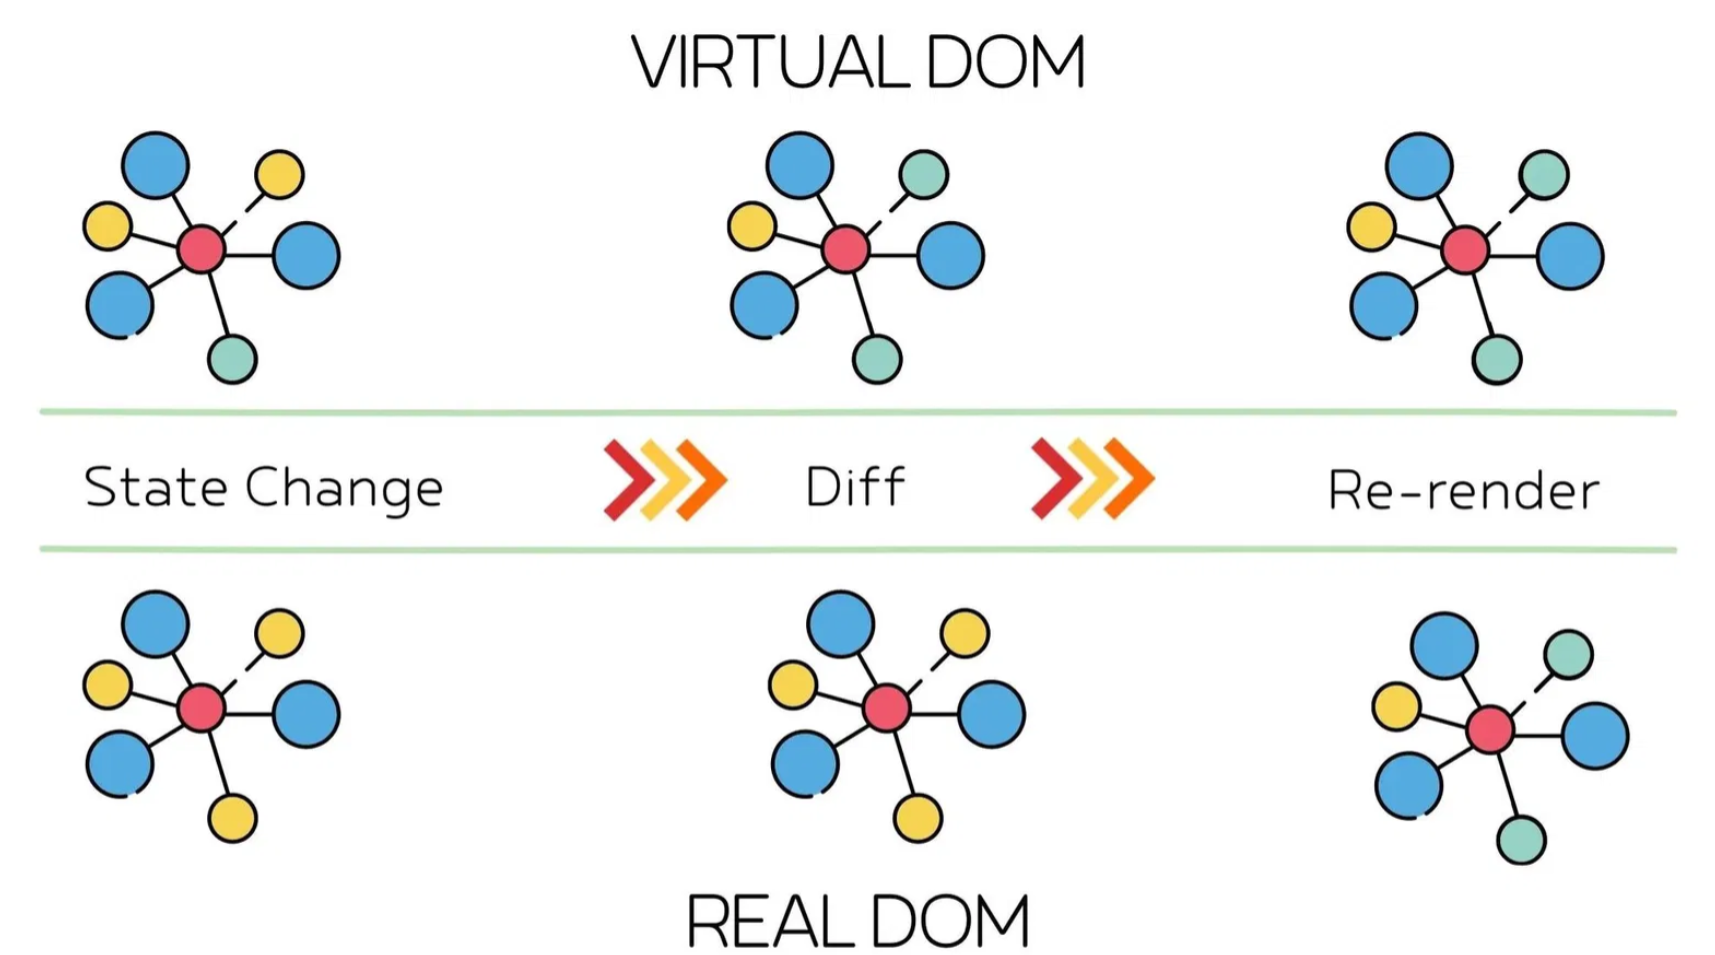
\includegraphics[scale=0.35]{img/Virtual-DOM.png}
    \caption{So sánh giữa DOM ảo (Virtual DOM) và DOM thật (Real DOM)}
    \label{fig:virtualDOM}
\end{figure}

Tuy nhiên, việc cập nhật DOM thật có thể gây ra tình trạng chậm chạp và kém hiệu quả đặc biệt là ở trong các ứng dụng lớn với nhiều phần tử. Vì vậy, React đã sử dụng DOM ảo với mục đích chỉ những phần có sự thay đổi mới được cập nhật lên DOM thật giúp tiết kiệm thời gian và tài nguyên.

\subsubsection{Redux Toolkit}
Đầu tiên, Redux là một thư viện quản lý trạng thái tương thích với các ứng dụng web. Đây là một công cụ hữu ích giúp bạn xây dựng các ứng dụng có tính nhất quán, hoạt động linh hoạt trên nhiều môi trường (client, server và native), và dễ dàng kiểm thử. Do sáng tạo từ ngôn ngữ Elm và kiến trúc Flux của Facebook,  do đó, Redux thường được kết hợp sử dụng cùng với React.

Redux có nhiệm vụ quản lý trạng thái phức trong ứng dụng web, giúp tách biệt logic và giao diện người dùng. Với việc tiếp cận dễ hiểu và dễ theo dõi, Redux sẽ giúp bạn theo dõi và cập nhật trạng thái một cách hiệu quả, đồng thời đảm bảo tính nhất quán của dữ liệu trong ứng dụng.

Tuy nhiên, một số lập trình viên cảm thấy Redux hơi dài dòng và khó sử dụng. Với những bất cập như việc tạo một store hoàn chỉnh cần đòi hỏi nhiều bước và tạo nhiều tệp lặp đi lặp lại. Nhằm tối giản hóa cách setup và sử dụng, Redux Toolkit được ra đời. Nó giúp các lập trình viên có thể tập trung hơn vào việc xử lý logic thay vì mất quá nhiều thời gian ban đầu để setup.

Redux Toolkit là một thư viện được phát triển bởi ReduxJS, giúp việc viết mã Redux nhanh chóng và toàn diện. Nó giải quyết vấn đề phức tạp của Redux và cung cấp API tiện ích để viết mã ngắn gọn, dễ đọc hơn. Ngoài ra, Redux Toolkit còn có nhiều lợi ích khác bên cạnh:

\begin{itemize}
    \item \textbf{Đơn giản hoá quy trình phát triển}: Redux Toolkit giúp giảm số lượng mã cần phải viết và đơn giản hoá các cú pháp. Điều này không chỉ giúp tiết kiệm thời gian mà còn làm cho mã nguồn trở nên dễ đọc và bảo trì tốt hơn.
    \item \textbf{Giảm thiểu mã lặp lại}: Một trong những vấn đề lớn khi sử dụng Redux là mã lặp lại. Redux Toolkit cung cấp các utility functions giúp bạn tạo ra reducers và actions một cách nhanh chóng và hiệu quả.
    \item \textbf{Hỗ trợ cho các tác vụ bất đồng bộ}: Redux Toolkit tích hợp sẵn các công cụ để xử lý các tác vụ bất đồng bộ thông qua createAsyncThunk. Điều này giúp bạn dễ dàng quản lý các yêu cầu API mà không cần phải viết nhiều mã phức tạp để xử lý trạng thái loading và error.
    \item \textbf{Tích hợp dễ dàng với React}: Redux Toolkit được thiết kế để hoạt động tốt với React, cung cấp các API như configureStore để dễ dàng cấu hình store và kết nối với các component. Điều này giúp bạn nhanh chóng tích hợp Redux vào ứng dụng React mà không gặp phải nhiều khó khăn.
    \item \textbf{Tăng cường hiệu suất}: Việc sử dụng Redux Toolkit giúp chuẩn hóa dữ liệu trước khi lưu vào Redux store, từ đó cải thiện hiệu suất của ứng dụng. Điều này đặc biệt quan trọng trong các ứng dụng lớn với nhiều state phức tạp.
\end{itemize}

\subsection{Vite}
Vite là một công cụ build và phát triển ứng dụng web được tạo ra bởi Evan You, người đã phát triển Vue.js, Vite ra đời mục đích khắc phục những hạn chế về tốc độ và hiệu suất. Nó cung cấp một cách tiếp cận mới để xây dựng các dự án web bằng cách tận dụng các mô-đun ES gốc trong trình duyệt và cung cấp tính năng thay thế mô-đun nóng (HMR) nhanh chóng. Tính năng này cho phép cập nhật tức thì mà không cần tải lại trang hoặc làm mất trạng thái ứng dụng, giúp quá trình phát triển hiệu quả hơn.

Các tính năng chính của Vite bao gồm:
\begin{itemize}
    \item \textbf{Tệp theo yêu cầu được phân phát qua ESM (Mô-đun ECMAScript) gốc}: giúp loại bỏ nhu cầu đóng gói. Tính năng này cải thiện đáng kể tốc độ và hiệu suất của các dự án phát triển web.
    \item \textbf{Thay thế mô-đun nóng (HMR)}: một tính năng cho phép các nhà phát triển thực hiện các thay đổi đối với mã của họ và xem kết quả ngay lập tức mà không cần phải tải lại toàn bộ trang. Điều này không chỉ tăng tốc quá trình phát triển mà còn nâng cao trải nghiệm người dùng bằng cách duy trì trạng thái ứng dụng.
    \item \textbf{Cung cấp API plugin và API JavaScript}: cho phép các nhà phát triển tùy chỉnh và mở rộng các chức năng của nó theo yêu cầu của dự án của họ. Tính linh hoạt này làm cho Vite.js trở thành một công cụ linh hoạt cho nhiều dự án phát triển web.
\end{itemize}

\subsubsection{So sánh giữa Webpack và Vite}
\begin{table}[H]
    \centering
    \begin{tabular}{|>{\centering\arraybackslash}p{0.18\linewidth}|>{\centering\arraybackslash}p{0.35\linewidth}|>{\centering\arraybackslash}p{0.35\linewidth}|} \hline 
         &  Vite& Webpack\\ \hline 
         Tốc độ khởi động&  	Khởi động nhanh nhờ sử dụng ES Modules gốc của trình duyệt, chỉ tải các tệp cần thiết.& Khởi động chậm hơn do phải đóng gói toàn bộ mã trước khi chạy.\\ \hline 
         Phản hồi khi thay đổi mã&  HMR (Hot Module Replacement) nhanh, mượt mà, chỉ cập nhật phần code thay đổi.& HMR khả dụng nhưng có thể chậm hơn, đặc biệt với mã nguồn phức tạp.
\\ \hline 
         Cấu hình&  Cấu hình đơn giản, thân thiện với người mới bắt đầu, có sẵn thiết lập cho các framework phổ biến.	& Cấu hình phức tạp, cần nhiều thiết lập thủ công để tối ưu.
\\ \hline 
         Hỗ trợ mở rộng và plugin&  Hỗ trợ API plugin mạnh mẽ, dễ tùy chỉnh và mở rộng theo nhu cầu dự án.& Plugin hỗ trợ mạnh mẽ nhưng có thể phức tạp và khó tích hợp hơn.
\\ \hline 
         Kích thước build cuối cùng&  Dùng Rollup để đóng gói, thường tạo ra các file nhỏ gọn và tối ưu.& Có thể tối ưu kích thước build nhưng cần nhiều cấu hình để đạt hiệu quả tốt nhất.
\\ \hline
    \end{tabular}
    \caption{Bảng so sánh giữa Webpack và Vite}
    \label{tab:Vite}
\end{table}

\subsection{Axios}
Axios là thư viện giúp client tương tác với server thông qua giao thức HTTP dựa trên các Promises, có thể chạy được trên cả trình duyệt và NodeJS (phía server). Về cơ bản, nó cung cấp một API cho việc xử lý XHR (XMLHttpRequests). Ở phía trình duyệt, Axios sử dụng XMLHttpRequest (XHR) cung cấp một API cho việc gọi và xử lý request/response lên server; ngược lại ở phía server thì Axios sử dụng native module http trong NodeJS để xử lý.

Promise API được hiểu là một tập hợp các phương thức và tính năng liên quan đến Promises trong JavaScript. Promises là một cơ chế xử lý bất đồng bộ được sử dụng để xử lý các hoạt động mà cần thời gian để hoàn thành, chẳng hạn như các yêu cầu HTTP, đọc/ghi vào tệp, hoặc tương tác với cơ sở dữ liệu.

Trong phần cấu hình Axios, Axios cung cấp sẵn cho chúng ta 2 lựa chọn để chuyển đổi dữ liệu:

\begin{itemize}
    \item \textbf{TransformResponse}: cho phép bạn chuyển đổi dữ liệu từ response trước khi nó được trả về cho bạn.
    \item \textbf{TransformRequest}: cho phép bạn chuyển đổi dữ liệu trước khi gửi nó đi.
\end{itemize}

Ngoài ra, Axios còn có một tính năng mạnh mẽ gọi là Interceptors. Nó cho phép bạn can thiệp vào quy trình gửi và tiếp nhận yêu cầu HTTP trước và sau khi chúng được gửi. Bạn có thể sử dụng Interceptors để thực hiện các tác vụ như thêm tiêu đề, xử lý lỗi, thêm hoặc xoá thông tin từ yêu cầu và phản hồi, và nhiều tác vụ khác.
Axios cũng có hỗ trợ hai loại Interceptor chính:
\begin{itemize}
    \item \textbf{Request Interceptors}: Được gọi trước khi yêu cầu được gửi đi. Bạn có thể sử dụng chúng để thêm tiêu đề, thêm token xác thực, hoặc xử lý dữ liệu yêu cầu trước khi nó được gửi.
    \item \textbf{Response Interceptors}: Được gọi sau khi yêu cầu đã được gửi và phản hồi đã được nhận. Bạn có thể sử dụng chúng để xử lý dữ liệu phản hồi, xử lý lỗi, và thực hiện các tác vụ khác trên phản hồi.
\end{itemize}
 
Lý do sử dụng Axios:
\begin{itemize}
    \item \textbf{Dễ sử dụng và bảo trì}: Axios cung cấp một cách gọi API dễ đọc và dễ sử dụng hơn so với việc sử dụng XMLHttpRequest. Cú pháp của Axios rõ ràng và giúp tạo ra những đoạn code dễ bảo trì hơn về sau.
    \item \textbf{Hỗ trợ Promise}: Axios sử dụng Promise, giúp bạn quản lý bất đồng bộ dễ dàng hơn. Bạn có thể sử dụng .then() và .catch() để xử lý phản hồi và lỗi.
    \item \textbf{Hỗ trợ Interceptor}: Axios cho phép bạn sử dụng interceptors để can thiệp vào quy trình gửi và nhận yêu cầu HTTP, điều này giúp bạn thực hiện các tác vụ như thêm tiêu đề, xử lý lỗi, và nhiều tác vụ khác một cách dễ dàng.
    \item \textbf{Hỗ trợ tự động chuyển đổi dữ liệu}: Axios cho phép bạn tự động chuyển đổi dữ liệu từ JSON, XML và nhiều định dạng khác thành các kiểu dữ liệu JavaScript phổ biến như đối tượng hoặc mảng.
    \item \textbf{Hỗ trợ huỷ yêu cầu}: Axios cung cấp tích hợp hỗ trợ hủy yêu cầu, cho phép bạn hủy các yêu cầu đang chờ khi không còn cần thiết, ngăn cản các yêu cầu không mong muốn.
    \item \textbf{Hỗ trợ Xác thực}: Axios dễ dàng tích hợp với các phương thức xác thực khác nhau, bao gồm xác thực cơ bản, mã thông báo Bearer, và nhiều hình thức xác thực khác.
    \item \textbf{Hỗ trợ gửi yêu cầu CORS}: Axios mặc định đã tích hợp sẵn hỗ trợ gửi yêu cầu qua CORS (Cross-Origin Resource Sharing) và cho phép bạn tùy chỉnh các tiêu đề CORS dễ dàng.
    \item \textbf{Khả năng tuỳ chỉnh cao}: Axios có tính tùy chỉnh cao, cho phép bạn cấu hình nhiều khía cạnh của quy trình gửi và nhận yêu cầu HTTP.
    \item \textbf{Thư viện phổ biến và cộng đồng lớn}: Axios là một thư viện phổ biến và được sử dụng rộng rãi trong cộng đồng phát triển, điều này có nghĩa bạn có thể tìm thấy nhiều tài liệu hữu ích và hỗ trợ từ cộng đồng.
\end{itemize}

\subsection{TailwindCSS}
TailwindCSS là một framework CSS utility-first giúp tạo kiểu nhanh chóng và hiệu quả cho website mà không cần viết CSS thủ công. Thay vì cung cấp các thành phần (component) hoặc kiểu thiết kế mặc định, Tailwind cung cấp một loạt các lớp tiện ích (utility classes) mà bạn có thể kết hợp linh hoạt để xây dựng giao diện tùy chỉnh.

Tailwind cung cấp một bộ các lớp CSS được đặt tên theo chức năng của chúng, cho phép bạn kiểm soát trực tiếp các khía cạnh như bố cục, màu sắc, khoảng cách, kiểu chữ và bóng đổ mà không cần viết CSS tùy chỉnh. 

TailwindCSS hoạt động tốt nhất khi bạn muốn sáng tạo và kiểm soát thiết kế trang web của mình. Nó đặc biệt hữu ích cho các thiết kế độc đáo, các tính năng tương tác và các dự án mà giao diện là điểm quan trọng nhất. 

Ưu điểm của TailwindCSS:
\begin{itemize}
    \item \textbf{Giảm thiểu viết CSS tuỳ chỉnh}: Bạn có thể chỉnh sửa style của các thành phần bằng cách áp dụng những class được xây dựng sẵn vào HTML. Bằng cách này, bạn có thể xây dựng các thiết kế tuỳ chỉnh mà không cần viết CSS.
    \item \textbf{Giữ cho file CSS gọn nhẹ}: Với những class được xây dựng sẵn dưới dạng component như vậy, hầu hết các style đều có thể được tái sử dụng.
    \item \textbf{Thay đổi an toàn}: Với cách tiếp cận truyền thống, nếu bạn thay đổi CSS rất có thể một phần nào đó trên trang web sẽ bị lỗi. Tuy nhiên với Tailwind, các lớp tiện ích trong HTML là cục bộ, nhờ đó mà bạn không làm thay đổi những phần khác trên trang web. 
    \item \textbf{Tính đáp ứng và bảo mật}: Với các lớp dựng sẵn của Tailwind, bạn có thể thiết kế bố cục trực tiếp trong một file HTML. Điều này biến Tailwind thành một framework CSS đáp ứng cao, thân thiện với thiết bị di động. 
    \item \textbf{Xây dựng các ứng dụng web có khả năng đáp ứng}: Tailwind CSS bao gồm các lớp tích hợp sẵn để tạo các giao diện đáp ứng. Bạn không cần phải viết thêm CSS để điều chỉnh giao diện cho các thiết bị khác nhau. 
    \item \textbf{Tương thích với các thư viện JavaScript phổ biến}: Tailwind CSS tương thích với các thư viện JavaScript phổ biến như React, Vue.js và Angular.
    \item \textbf{Kiểm soát hoàn toàn đối với giao diện người dùng}: Tailwind CSS cung cấp cho bạn sự linh hoạt cao để tạo giao diện tùy chỉnh theo ý muốn. Bạn không bị giới hạn bởi các thành phần được thiết kế sẵn như trong các framework CSS khác. 
\end{itemize}

Nhược điểm của TailwindCSS:
\begin{itemize}
    \item \textbf{Quá trình đánh dấu (markup) trở nên dài dòng}: Không giống như các framework CSS khác, Tailwind hoạt động bằng cách trộn lẫn các quy tắc kiểu dáng trực tiếp vào các file HTML. Mặc dù điều này có lợi cho những người không quen thuộc với CSS nhưng nó cũng đi ngược lại nguyên tắc “phân tách mối quan tâm” (separation of concerns) trong lập trình, làm cho quá trình đánh dấu (markup) trở nên dài dòng. 
    \item \textbf{Cần nhiều thời gian để học tập}: Do Tailwind CSS có nhiều lớp tiện ích tích hợp nên thời gian để học tập và thành thạo là rất dài. Ngay cả với các developer giàu kinh nghiệm, việc sử dụng và tận dụng tối đa các lớp dựng sẵn cũng có thể là một thách thức. 
    \item \textbf{Thiếu các thành phần quan trọng}: Không giống như Bulma và Bootstrap, Tailwind không cung cấp nhiều thành phần giao diện (UI) quan trọng. Điều này có nghĩa là bạn phải tự thêm các tính năng như header, button và thanh điều hướng cho các ứng dụng web. 
    \item \textbf{Chưa có nhiều tài liệu để học tập}: Mặc dù tài liệu tham khảo về Tailwind CSS đã bổ sung các video và tài liệu hướng dẫn, nhưng vẫn chưa đầy đủ như các đối thủ cạnh tranh như Bootstrap. 
    \item \textbf{Kích thước bundle lớn}: Tailwind CSS có thể có bundle lớn hơn so với các framework CSS khác, ảnh hưởng đến hiệu suất trang web, đặc biệt trên mạng chậm. 
    \item \textbf{Bảo trì khó khăn}: Việc bảo trì các ứng dụng web được xây dựng bằng Tailwind CSS có thể khó khăn hơn do markup có thể trở nên dài dòng và khó đọc. \\
\end{itemize}

\subsubsection{So sánh giữa TailwindCSS và Bootstrap}
Bootstrap là một bộ công cụ mã nguồn mở miễn phí, được sử dụng để thiết kế giao diện người dùng (UI) cho các trang web. Framework này bao gồm các thành phần HTML, CSS và JavaScript được tạo sẵn. 

Bootstrap là một framework HTML, CSS và JavaScript miễn phí dùng để tạo website và web application. Bootstrap được phát triển bởi Mark Otto và Jacob Thornton của Twitter, giúp cho việc phát triển web trở nên nhanh chóng và dễ dàng hơn.

Chúng tương thích hoàn hảo với các trình duyệt (IE, Firefox và Chrome) và phù hợp với mọi kích cỡ màn hình (máy tính bàn, máy tính bảng, điện thoại). Với Bootstrap, người dùng không cần phải có kiến thức chuyên sâu về CSS hay HTML để thiết kế một trang web đẹp và hiệu quả.

Tuy nhiên, có sự khác nhau giữa Boostrap và TailwindCSS:
\begin{table}[H]

    \centering
    \begin{tabular}{|>{\centering\arraybackslash}p{0.15\linewidth}|>{\centering\arraybackslash}p{0.3\linewidth}|>{\centering\arraybackslash}p{0.45\linewidth}|} \hline 
         Tính năng&  Boostrap& TailwindCSS\\ \hline 
         Tính linh hoạt&  Cung cấp các thành phần sẵn có.& Cho phép tinh chỉnh và thay đổi mọi thứ một cách tự do.\\ \hline 
         Hiệu suất&  Có thể tạo ra CSS bundle lớn hơn do bao gồm nhiều thành phần UI được thiết kế sẵn.& Có thể tạo ra CSS bundle nhỏ hơn so với Bootstrap, dẫn đến hiệu suất trang web tốt hơn.
\\ \hline 
         Thời gian học tập&  Dễ dàng cho người mới bắt đầu.	
& Cần nhiều thời gian học tập hơn.

\\ \hline 
         Lợi ích học tập&  Làm quen với các thành phần sẵn có.	& Học cách sử dụng các kiểu nhỏ, có thể tái sử dụng trong toàn bộ thiết kế.
\\ \hline 
         Tài liệu học tập&  Có nhiều tài liệu hướng dẫn, video hướng dẫn, khóa học trực tuyến miễn phí và trả phí.& 
Cộng đồng đang phát triển nhanh chóng nhưng tài liệu hướng dẫn chính thức và các nguồn tài nguyên học tập có thể hạn chế hơn so với Bootstrap. Tuy nhiên, có nhiều bài viết, video, khoá học do cộng đồng tạo ra để hỗ trợ bạn.
\\ \hline 
         Templates và Themes&  Nhiều thiết kế sẵn bao gồm miễn phí và trả phí.& 
Số lượng template và theme ít hơn, nhưng bạn có thể dễ dàng tạo giao diện tùy chỉnh theo ý muốn.\\ \hline 
         Plugin và Extension&  Có các công cụ bổ sung cho nhiều tính năng hơn như lịch, trình chiếu và hoạt ảnh.& Cộng đồng đang phát triển các plugin và extension mới nhưng số lượng vẫn hạn chế so với Bootstrap. Tuy nhiên, bạn có thể sử dụng các JavaScript khác để bổ sung chức năng cho ứng dụng của mình.\\ \hline 
         Công cụ tích hợp&  Tương thích tốt với jQuery và các công cụ hiện đại như React và Angular.& Tương thích tốt với PostCSS và các công cụ JavaScript.\\ \hline 
         Tương thích trình duyệt&  Lựa chọn tốt hơn nếu bạn cần trang web hoạt động trên các trình duyệt cũ. & 
Tập trung vào các trình duyệt hiện đại, nhưng vẫn tương thích tốt với hầu hết trình duyệt phổ biến.
\\ \hline
    \end{tabular}
    \caption{Bảng so sánh Boostrap và TailwindCSS}
    \label{tab:TailwindCSS}
\end{table}

\subsection{Material UI}
Material UI là một thư viện React phổ biến, cung cấp các thành phần giao diện người dùng (UI) được thiết kế theo phong cách Material Design của Google. Nó giúp các nhà phát triển xây dựng các ứng dụng web với giao diện đẹp mắt và nhất quán một cách nhanh chóng và dễ dàng.

Material UI đem đến cho bạn và trang web của bạn một giao diện hoàn toàn mới, với những button, textfield, toggle... được design theo một phong cách mới lạ, thay thế việc sử dụng các framework khác như Bootstrap.

Có 2 theme cơ bản trong Material UI là light-theme và dark-theme. Light theme cho trang web của bạn phông nền trắng còn ngược lại dark-theme sẽ là phồng nền đen. Bắt đầu từ phiên bản 0.8.0 thì việc khai báo sử dụng theme là bắt buộc đối bới Material UI. Material UI cũng cung cấp cho bạn khả năng chỉnh sửa lại theme.

\section{Phát triển back-end}
Phát triển back-end là một phần quan trọng trong quy trình phát triển phần mềm, tập trung vào việc xây dựng và duy trì các hệ thống máy chủ, cơ sở dữ liệu, và các API mà người dùng không trực tiếp thấy nhưng đóng vai trò quyết định đến sự vận hành của ứng dụng. Trong khi front-end xử lý mọi thứ mà người dùng có thể tương tác, back-end chịu trách nhiệm xử lý logic ứng dụng, lưu trữ và truy xuất dữ liệu, cũng như đảm bảo rằng tất cả các yếu tố của hệ thống hoạt động đồng bộ và hiệu quả.

Phát triển back-end là nền tảng vững chắc cho bất kỳ ứng dụng hoặc hệ thống nào. Công việc này yêu cầu khả năng giải quyết vấn đề, tối ưu hóa hiệu suất và bảo mật, đồng thời đảm bảo sự đồng bộ giữa các phần khác nhau của ứng dụng. Đây là lĩnh vực không thể thiếu trong phát triển phần mềm, tạo ra những trải nghiệm người dùng mượt mà và hiệu quả.

\subsection{NodeJS}
NodeJS là một nền tảng được xây dựng trên “V8 Javascript engine” được viết bằng C++ và Javascript. Nền tảng này được phát triển bởi Ryan Lienhart Dahl vào năm 2009. NodeJS ra đời khi các developer đời đầu của JavaScript mở rộng nó từ một thứ bạn chỉ chạy được trên trình duyệt thành một thứ bạn có thể chạy trên máy của mình dưới dạng ứng dụng độc lập. Động cơ JavaScript được phát triển bởi Google cho trình duyệt Chrome, đây là một động cơ rất nhanh cho phép biên dịch mã JavaScript thành mã máy để thực thi trực tiếp trên phần cứng, làm tăng hiệu suất thực thi. Điều này giúp Node.js có khả năng thực thi JavaScript nhanh và hiệu quả, đồng thời hỗ trợ các tính năng mới nhất của ngôn ngữ JavaScript.

NodeJS đã mở rộng khả năng của JavaScript từ việc chỉ phát triển front-end trong trình duyệt để bao gồm cả phát triển back-end. Điều này có nghĩa là các lập trình viên có thể sử dụng cùng một ngôn ngữ lập trình, JavaScript, để phát triển toàn bộ ứng dụng, từ front-end đến back-end, qua đó tạo điều kiện cho việc học tập và phát triển ứng dụng nhanh chóng và hiệu quả hơn.

NodeJS hoạt động dựa trên một số nguyên tắc cơ bản giúp nó hiệu quả trong việc xử lý các ứng dụng có nhiều hoạt động nhập/xuất (I/O) mà không bị chặn, đồng thời giảm đáng kể sự phức tạp trong quản lý các luồng thực thi.

NodeJS sử dụng một mô hình non-blocking I/O (input/output) và event-driven, nghĩa là các hoạt động như đọc file, truy vấn cơ sở dữ liệu, hoặc giao tiếp mạng được thực hiện mà không chặn tiến trình chính. Điều này cho phép xử lý nhiều yêu cầu cùng lúc mà không cần tạo nhiều luồng (thread), giúp giảm bớt chi phí liên quan đến quản lý luồng và tối ưu hóa hiệu suất. Khi một hoạt động I/O được khởi tạo, nó sẽ được gửi đến thực thi trong hệ thống hoặc cơ sở dữ liệu mà không làm chậm tiến trình chính. Sau khi hoạt động hoàn tất, một sự kiện sẽ được phát đi và xử lý bằng các hàm gọi lại (callback).

\begin{figure}[H]
    \centering
    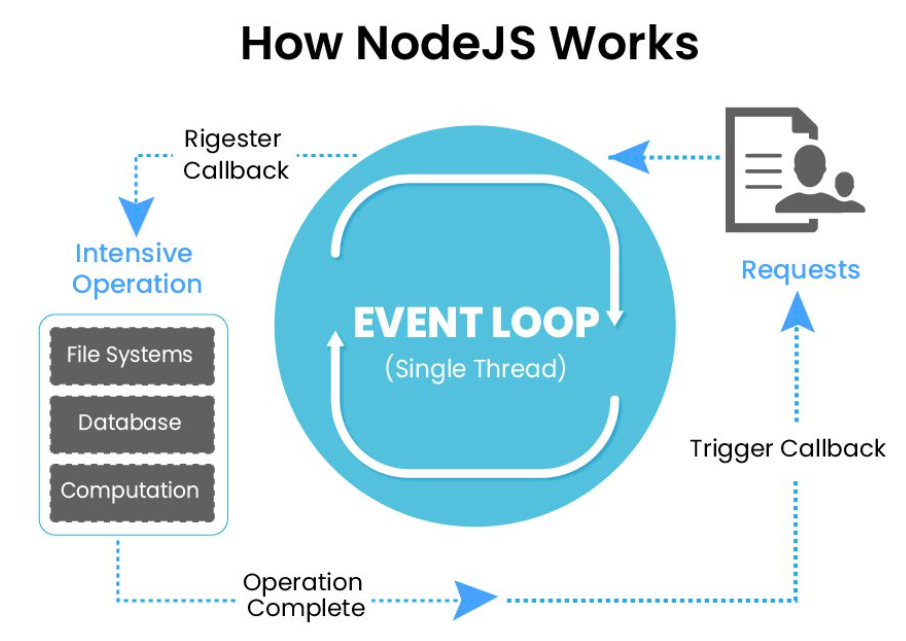
\includegraphics[scale=0.5]{img/NodeJS-work.png}
    \caption{Cách vận hành của NodeJS}
    \label{fig:nodejs}
\end{figure}

Mặc dù Node.js hoạt động trên một luồng duy nhất cho logic ứng dụng của người dùng, nó vẫn sử dụng nhiều luồng ở tầng thấp hơn thông qua thư viện "libuv" để xử lý các hoạt động I/O. Trái tim của Node.js là “event loop”. Đây là vòng lặp sự kiện mà ở đó Node.js tiếp tục lắng nghe sự kiện và thực hiện các hàm gọi lại khi một sự kiện được kích hoạt. Vòng lặp sự kiện cho phép Node.js xử lý hàng nghìn kết nối đồng thời mà không cần phải tạo ra chi phí quản lý luồng. Khi thao tác I/O hoàn tất, hệ điều hành thông báo cho Node.js, và Node.js sau đó thực thi hàm callback tương ứng để xử lý kết quả hoặc tiếp tục xử lý logic.

\subparagraph{Ưu điểm của NodeJS:}
\begin{itemize}
    \item \textbf{Hiệu suất cao:} Nodejs chạy đơn luồng, sử dụng V8 Engine, giúp ứng dụng đảm bảo tốc độ khi có nhiều requests. 
    \item \textbf{Xử lý bất đồng bộ và I/O hướng sự kiện:} Khả năng xử lý I/O bất đồng bộ, giúp Nodejs có thể xử lý nhiều tasks, mà không cần phải chờ kết quả của task trước đó. 
    \item \textbf{Phát triển ứng dụng:} Có thể sử dụng để phát triển ứng dụng ở cả phía client và server. 
    \item \textbf{Module đa dạng:} Nodejs sở hữu một cộng đồng duy trì, phát triển modules, thư viện giúp cho việc phát triển ứng dụng nhanh chóng.
    \item \textbf{Stream và xử lý file lớn:} Nodejs hỗ trợ streaming, cho phép xử lý các file có kích thước lớn không tốn nhiều tài nguyên.
    \item \textbf{Phù hợp với ứng dụng real time:} Do Nodejs xử lý bất đồng bộ, thích hợp với các ứng dụng real time như: chat applications, streaming services,...
    \item \textbf{Hệ sinh thái phong phú}: Với hơn 50,000 gói có sẵn trong Node Package Manager (NPM), các nhà phát triển có thể dễ dàng tìm và sử dụng các thư viện theo nhu cầu của họ mà không cần phải viết lại từ đầu, tiết kiệm đáng kể thời gian và công sức.
    \item \textbf{Tính nhất quán trong mã nguồn}: NodeJS cho phép sử dụng cùng một ngôn ngữ lập trình (JavaScript) cho cả phía máy chủ và máy khách. Điều này không chỉ giúp giảm thiểu sự không đồng bộ giữa client và server mà còn làm cho việc bảo trì và quản lý mã nguồn trở nên dễ dàng hơn.
 
\end{itemize}

Nhược điểm của NodeJS:
\begin{itemize}
    \item Cần có kiến thức nền tảng về JavaScript.
    \item Khá phức tạp trong việc thao tác với cơ sử dữ liệu quan hệ.
    \item Mỗi callback sẽ đi kèm với rất nhiều callback lồng nhau khác, dễ dẫn đến tình trạng "callback hell".
    \item Không phù hợp với các tác vụ đòi hỏi nhiều CPU core.
\end{itemize}

\subsection{ExpressJS}

ExpressJS là một framework được xây dựng trên nền tảng của NodeJS. Nó cung cấp các tính năng mạnh mẽ để phát triển web hoặc mobile. ExpressJS hỗ trợ các method HTTP và middleware tạo ra API vô cùng mạnh mẽ và dễ sử dụng. Với ExpressJS, bạn có thể xây dựng các API RESTful dễ dàng hơn và quản lý dữ liệu hiệu quả mà không cần viết quá nhiều code phức tạp. ExpressJS giúp bạn tập trung vào logic ứng dụng thay vì xử lý chi tiết các yêu cầu HTTP.

ExpressJS tập trung vào công việc tối ưu hóa việc xây dựng web ứng dụng bằng cách cung cấp một cấu trúc hoạt động và chỉ định rõ ràng việc xử lý yêu cầu và phản hồi. Nền tảng cũng hỗ trợ tích hợp các phần mềm trung gian bên ngoài để mở rộng chức năng của ứng dụng. 

\begin{figure}[H]
    \centering
    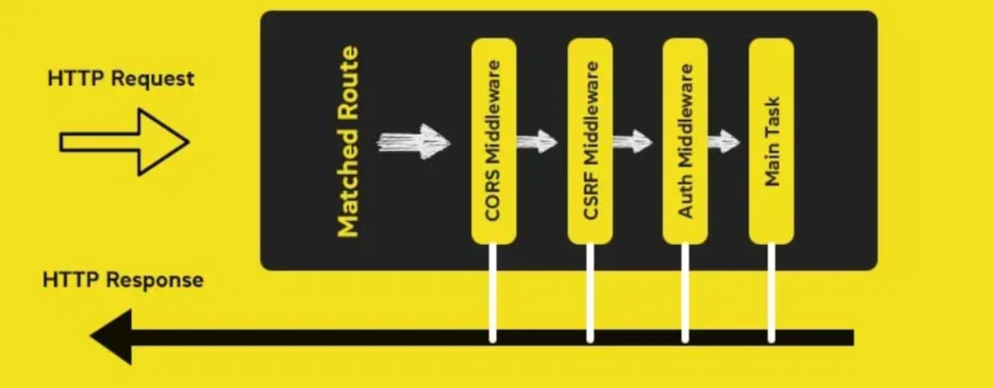
\includegraphics[scale=0.5]{img/ExpressJS-workflow.png}
    \caption{Luồng thực thi của ExpressJS}
    \label{fig:expressjs}
\end{figure}

Express.js hỗ trợ xây dựng API tuân thủ các nguyên tắc của kiến trúc REST (Representational State Transfer) thông qua việc thiết lập các route tương ứng với từng yêu cầu. API này sẽ bao gồm các tính năng như:
\begin{itemize}
    \item Xem danh sách tất cả sản phẩm.
    \item Xem thông tin chi tiết của một sản phẩm.
    \item Thêm một sản phẩm mới.
    \item Cập nhật thông tin sản phẩm.
    \item Xóa sản phẩm.
\end{itemize}

Các tính năng chính của ExpressJS:
\begin{itemize}
    \item \textbf{Định tuyến (Routing)}: cung cấp cơ chế hoạt động cơ bản để xác định điểm cuối và xử lý các yêu cầu HTTP đến từ các công cụ đường dẫn. Công việc quản lý định tuyến giúp xử lý logic yêu cầu riêng biệt cho từng phần của ứng dụng (GET, POST, PUT, DELETE,...), từ đó tạo điều kiện cho việc mở rộng và bảo trì một cách dễ dàng.
    \item \textbf{Middleware}: là hàm đặc biệt cho ExpressJS, cho phép thực thi các thao tác trung gian trước khi yêu cầu đến điểm cuối. Nó cho phép người dùng xác thực, xử lý lỗi, quản lý phiên, nén dữ liệu và nhiều tác vụ khác. 
    \item \textbf{Hỗ trợ công cụ mẫu (Templating Engine)}: hỗ trợ nhiều công cụ mẫu phổ biến nhằm tạo ra các trang HTML động trở nên dễ dàng và linh hoạt. VD: EJS (cho phép nhúng JavaScript trực tiếp vào HTML), Pug (Cung cấp cú pháp ngắn gọn, dễ đọc hơn để tạo HTML), Handlebars và Mustache (sử dụng để quản lý views và tạo HTML)
    \item \textbf{Quản lý tệp và dữ liệu tĩnh}: Middleware express.static() giúp việc phục vụ các tệp tĩnh trong dự án trở nên đơn giản. ExpressJS sẽ tự động xử lý việc cung cấp chúng cho người dùng khi họ yêu cầu.
\end{itemize}

\subsection{MongoDB}
MongoDB là một hệ thống cơ sở dữ liệu phi quan hệ (NoSQL database), mã nguồn mở được phát triển bới MongoDB Inc. Do là một database hướng tài liệu (document), một dạng của NoSQL database, vì thế, MongoDB tránh cấu trúc table-based của relational database để thích ứng với các tài liệu như JSON có schema rất linh hoạt gọi là BSON nên mỗi một collection sẽ các các kích cỡ và các document khác nhau. Các dữ liệu được lưu trữ trong document kiểu JSON nên truy vấn sẽ rất nhanh.

\begin{figure}[htp!]
    \centering
    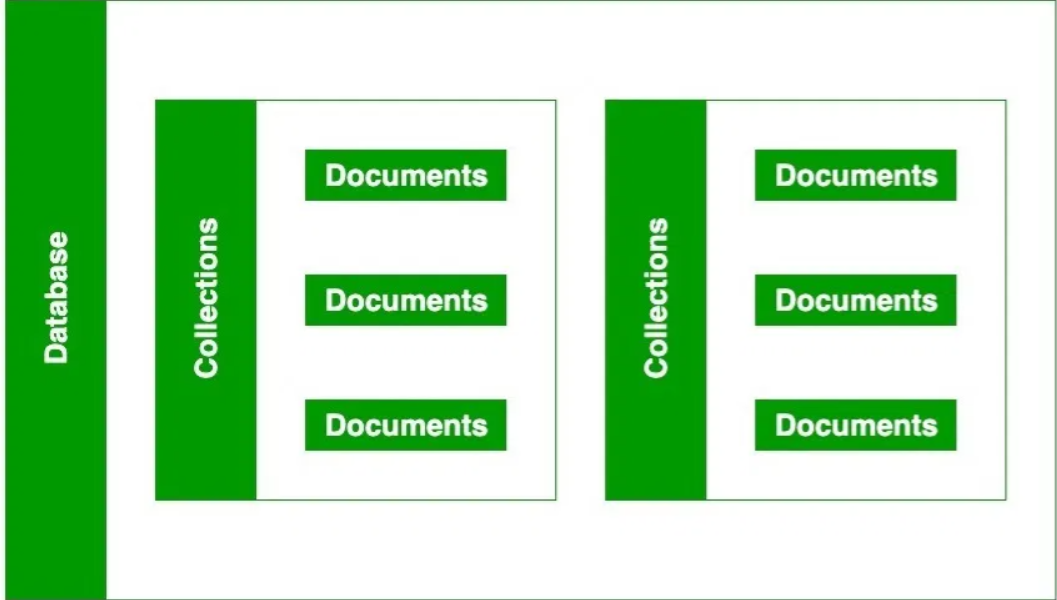
\includegraphics[scale=0.5]{img/MongoDB_work.png}
    \caption{Các thành phần trong MongoDB}
    \label{fig:mongodb}
\end{figure}

MongoDB hỗ trợ tất cả các ngôn ngữ phổ biến như C, C++, C\# và .Net, Go, Java, NodeJS, Perl, PHP, Python, Motor, Ruby, Scala, Swift, Mongoid. Vì vậy, MongoDB đã trở thành một trong những NoSQL database nổi trội nhất bấy giờ, được dùng làm backend cho rất nhiều website như eBay, SourceForge, The New York Times, Facebook, Nokia, eBay, Adobe, Google,... để lưu trữ lượng lớn dữ liệu của họ.

MongoDB không chỉ đơn thuần là một cơ sở dữ liệu, mà còn là một hệ sinh thái hoàn chỉnh với nhiều tính năng và công cụ hỗ trợ. Các tính năng và ưu điểm của MongoDB làm cho việc lưu trữ và xử lý dữ liệu trở nên dễ dàng và hiệu quả hơn, đáp ứng nhu cầu trong nhiều lĩnh vực, đặc biệt là trong Data analyst. Data analyst có thể sử dụng MongoDB để lưu trữ, xử lý và truy vấn các loại dữ liệu khác nhau. Ngoài ra, MongoDB cũng cung cấp các công cụ để truy vấn dữ liệu, tạo báo cáo và thực hiện các phân tích dữ liệu phức tạp cho data analyst. Vì vậy, có thể nói rằng MongoDB là một công cụ hữu ích cho data analyst trong việc lưu trữ và phân tích dữ liệu.

\subparagraph{Các tính năng chính của MongoDB:}
\begin{itemize}
    \item \textbf{Schema-less Database:} giúp tăng tính linh hoạt và giảm thời gian phát triển các ứng dụng, đặc biệt là đối với các ứng dụng có tính chất thay đổi dữ liệu thường xuyên hoặc không có một cấu trúc dữ liệu cố định. Do đó, bạn có thể lưu trữ các tài liệu với các fields và giá trị (values) khác nhau mà không cần tuân theo một cấu trúc cố định và không cần yêu cầu sự định nghĩa trước về cấu trúc của chúng. Tuy nhiên, tính năng này sẽ dẫn đến khó khăn trong việc truy vấn và xử lý dữ liệu nếu không có sự quản lý và thiết kế cẩn thận.
    \item \textbf{Document Oriented:} MongoDB được thiết kế để lưu trữ dữ liệu dưới dạng tài liệu (document). Mỗi tài liệu trong MongoDB được lưu trữ dưới một bản ghi độc lập bao gồm các fields (key-value pair) và giá trị tương ứng.
    \item \textbf{Indexing:} MongoDB tạo ra index để tăng tốc độ truy vấn và tìm kiếm dữ liệu trong cơ sở dữ liệu. Khi truy vấn dữ liệu, MongoDB sử dụng các Index để nhanh chóng tìm kiếm và trả về các tài liệu phù hợp với tiêu chí truy vấn. Việc sử dụng Index giúp giảm thời gian truy vấn tìm kiếm dữ liệu, đồng thời giúp tăng hiệu suất và khả năng mở rộng của MongoDB.
    \item \textbf{Replication:} là quá trình đồng bộ dữ liệu giữa các node trong một cluster MongoDB. Một cluster MongoDB sẽ gồm một node primary và nhiều node secondary. Node primary sẽ chịu trách nhiệm ghi dữ liệu mới vào cơ sở dữ liệu, còn các node secondary chỉ đọc dữ liệu. Với tính năng Replication, MongoDB có khả năng tự động sao lưu dữ liệu, đảm bảo độ tin cậy và khả năng phục hồi của cơ sở dữ liệu, đồng thời giúp tăng khả năng mở rộng của hệ thống.
    \item \textbf{Sao lưu và phục hồi:} MongoDB cung cấp tính năng sao lưu và phục hồi dữ liệu linh hoạt, cho phép lưu trữ các bản sao của dữ liệu và phục hồi dữ liệu trong trường hợp xảy ra sự cố.
    \item \textbf{Bảo mật:} MongoDB hỗ trợ nhiều tính năng bảo mật, bao gồm chứng thực người dùng (user authentication), mã hóa dữ liệu (data encryption) và kiểm soát quyền truy cập (access control).
\end{itemize}

\subsubsection{Ưu điểm của MongoDB:}
\begin{itemize}
    \item \textbf{Linh hoạt:} Do là một hệ thống cơ sở dữ liệu phi quan hệ nên nó cung cấp khả năng lưu trữ dữ liệu bất cứ khi nào, bất cứ nơi đâu, không cần phải tuân thủ một mô hình quan hệ cụ thể.
    \item \textbf{Khả năng mở rộng:} Nhờ tính năng sharding cho phép phân chia dữ liệu thành nhiều phần và lưu trữ trên nhiều máy chủ, nên MongoDB có khả năng mở rộng dễ dàng.
    \item \textbf{Tốc độ truy xuất nhanh:} MongoDB có thể đáp ứng các yêu cầu truy vấn dữ liệu trong thời gian ngắn hơn so với các hệ thống cơ sở dữ liệu quan hệ truyền thống.
    \item \textbf{Tính khả dụng cao:} MongoDB cung cấp tính năng sao lưu và phục hồi dữ liệu, giúp người dùng bảo vệ dữ liệu của mình khỏi những rủi ro.
    \item \textbf{Dễ dùng và tích hợp:} MongoDB cung cấp các công cụ quản lý dữ liệu trực quan và dễ sử dụng, giúp người dùng tối ưu hóa hiệu suất và quản lý cơ sở dữ liệu một cách dễ dàng. Đồng thời, dễ dàng tích hợp với Big Data Hadoop.
\end{itemize}

\subsubsection{Nhược điểm của MongoDB:}
\begin{itemize}
    \item Cần sử dụng bộ nhớ cao để lưu trữ dữ liệu (data storage).
    \item Không được phép lưu trữ hơn 16MB data trong tài liệu (do sử dụng BSON).
    \item Data nesting trong BSON cũng bị hạn chế, bạn không được phép nest data quá 100 cấp độ.
\end{itemize}

\subsubsection{So sánh MongoDB và MySQL:}
\begin{figure}[H]
    \centering
    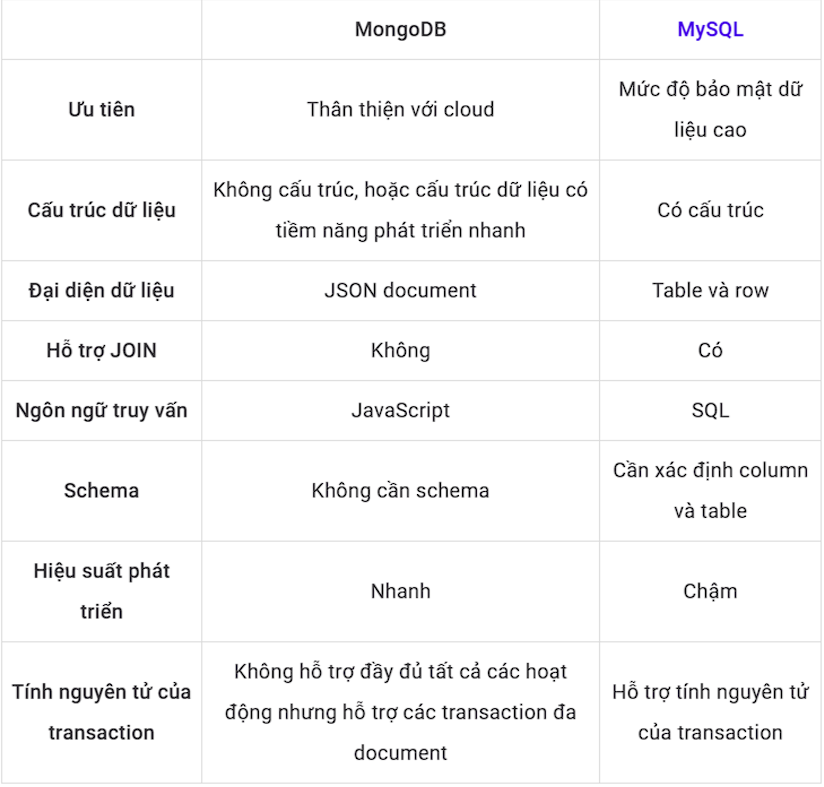
\includegraphics[width=0.8\textwidth]{img/MongoDB_MySQL_comparision.png}
    \caption{So sánh giữa MongoDB và MySQL}
    \label{fig:mongodb_mysql_comparison}
\end{figure}

\section{Phát triển server}
Phát triển server  (máy chủ) là một phần quan trọng trong quá trình xây dựng và triển khai ứng dụng web hoặc hệ thống phần mềm. Nó liên quan đến việc thiết kế, xây dựng, triển khai và duy trì các server - những hệ thống phần cứng hoặc phần mềm chịu trách nhiệm xử lý, lưu trữ và truyền tải dữ liệu giữa người dùng và ứng dụng. Mục tiêu của phát triển server là đảm bảo hệ thống hoạt động ổn định, có khả năng mở rộng và xử lý một lượng lớn yêu cầu từ người dùng.

\subsection{React Server Components (RSC)}
React Server Components (RSC) là một tính năng mới trong React, cho phép các component của React chạy hoàn toàn trên server thay vì trên client. Điều này giúp tối ưu hiệu năng, giảm tải công việc cho client, và tăng tốc độ tải trang.

RSC đặc biệt phù hợp cho các ứng dụng web phức tạp, nơi mà hiệu suất là yếu tố quan trọng. Các ứng dụng như nền tảng thương mại điện tử, ứng dụng truyền thông xã hội, hoặc các ứng dụng cần xử lý lượng dữ liệu lớn từ server sẽ hưởng lợi nhiều từ RSC.

React được tạo ra để kết hợp và áp dụng gia tăng vào các codebases hiện có. RSC mở rộng các nguyên tắc cơ bản của React vượt ra ngoài việc chỉ là một thư viện render, bằng cách tích hợp việc lấy dữ liệu và giao tiếp từ xa giữa client-server trong framework. RSCs tự động lấy dữ liệu và render hoàn toàn trên máy chủ, và kết quả HTML được truyền vào React component tree phía client, xen kẽ với các Server và Client Components khác khi cần thiết. Quá trình này loại bỏ nhu cầu render lại phía client, từ đó cải thiện hiệu suất. Khi một RSC cần được render lại do sự thay đổi trạng thái, nó sẽ làm mới trên server và hợp nhất vào DOM hiện có mà không cần làm mới toàn bộ trang. Kết quả là, trạng thái client được giữ nguyên ngay cả khi các phần của giao diện được cập nhật từ máy chủ.

\subsubsection{Quy trình làm việc khi không có RSC và khi có RSC:}

\begin{figure}[H]
    \centering
    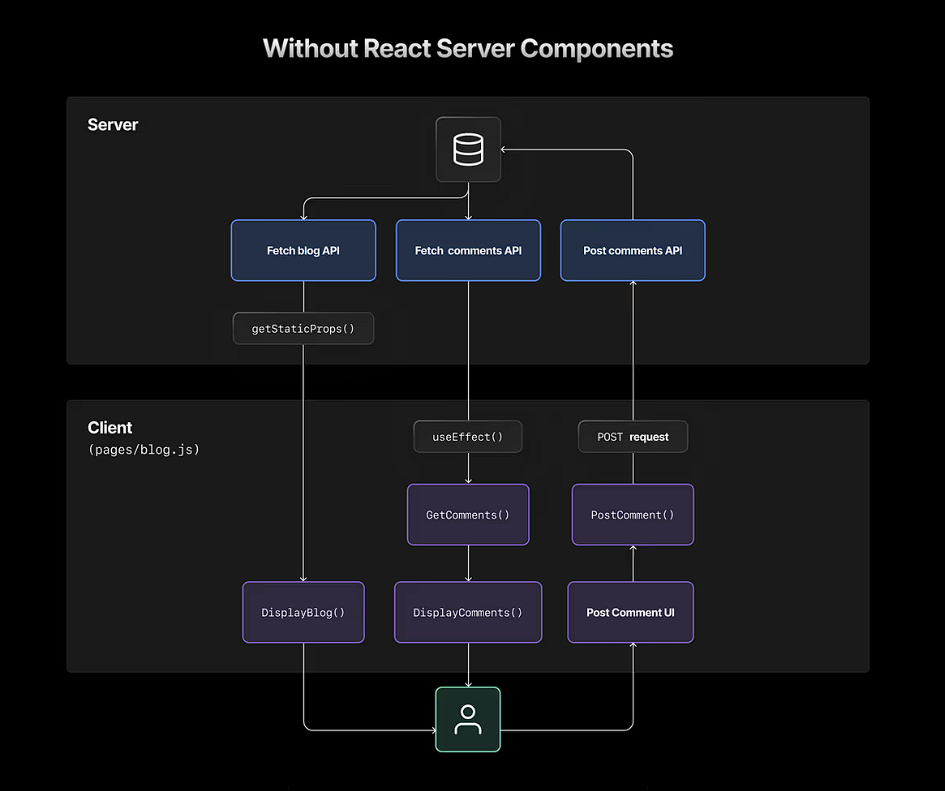
\includegraphics[width=0.8\textwidth]{img/withoutRSCs.png}
    \vspace{0.5cm}
    \caption{Khi không có RSC}
\end{figure}

\begin{figure}[H]
    \centering
    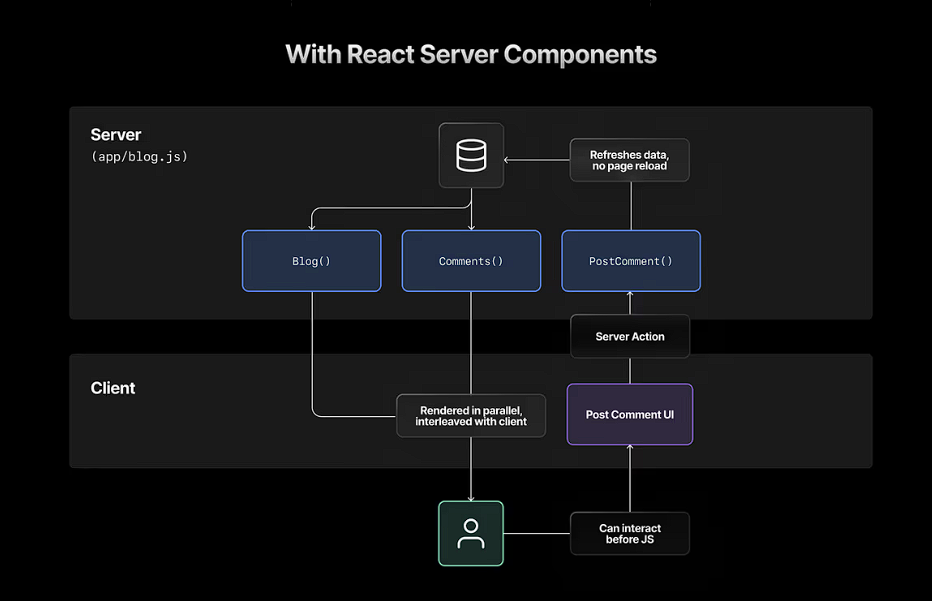
\includegraphics[width=0.8\textwidth]{img/withRSCs.png}
    \vspace{0.5cm}
    \caption{Khi có RSC}
\end{figure}

Như chúng ta có thể thấy, khi không có React Server Component (RSC) thì việc lấy dữ liệu cần thêm một layer API. Còn với khi có thêm React Server Component việc lấy dữ liệu và render giao diện người dùng (UI) có thể được thực hiện từ cùng một component và Server Actions cũng sẽ cung cấp phương pháp giúp cho người dùng có thể tương tác với dữ liệu phía máy chủ trước khi JavaScript tải trên trang. 

\subparagraph{Ưu điểm của React Server Components:}
\begin{itemize}
    \item \textbf{Tăng hiệu suất:} Nhờ vào việc giảm lượng JavaScript cần tải và xử lý trên client.
    \item \textbf{Thân thiện với SEO:} Nội dung được render trên server dễ dàng cho các công cụ tìm kiếm thu thập và lập chỉ mục hơn. 
    \item \textbf{Cải thiện trải nghiệm người dùng}: Tăng tốc độ tải trang và tăng tính tương tác của ứng dụng. 
\end{itemize}

\subsection{Vercel}

Vercel là một cloud platform (nền tảng đám mây) được tạo ra nhằm phục vụ việc phát triển và triển khai ứng dụng web nhanh chóng và dễ dàng. Nền tảng này cho phép bạn xây dựng, triển khai và quản lý các ứng dụng web mà không cần quan tâm đến việc cấu hình hệ thống máy chủ. Vercel hỗ trợ các ứng dụng web được viết bằng nhiều ngôn ngữ lập trình và nhiều framework khác nhau, như JavaScript, TypeScript, Python, Go,.... Với khả năng tự động hóa quá trình triển khai với CI/CD (Continuous Integration/Continuous Deployment), nó giúp các lập trình viên có thể triển khai mã nguồn của mình một cách nhanh chóng chỉ với vài thao tác đơn giản. 

Nó cung cấp 3 tính năng chính: deploy dễ dàng, preview trực tiếp và deliver đến khách hàng nhanh chóng.

\subparagraph{Ưu điểm của Vercel:}
\begin{itemize}
    \item \textbf{Tích hợp với Git:} Khi bạn kết nối tài khoản Github / Gitlab với Vercel, hệ thống sẽ tự động deploy mỗi khi có sự thay đổi trong nhánh chính của repository của bạn. Điều này giúp giảm thời gian triển khai và giảm tải cho bạn. Tích hợp với Git còn giúp cho quá trình phát triển và bảo trì mã nguồn trở nên mượt mà và hiệu quả hơn bởi việc sử dụng các tính năng của Git.
    \item \textbf{Hỗ trợ nhiều ngôn ngữ:} Vercel hỗ trợ nhiều ngôn ngữ lập trình, bao gồm JavaScript, React, Next.js, và nhiều ngôn ngữ khác.
    \item \textbf{Tốc độ nhanh:} Vercel cung cấp tốc độ tải nhanh và độ trễ thấp do có hệ thống phân tán tải nặng rộng rãi trên toàn thế giới, giúp cho trải nghiệm của người dùng tốt hơn.
    \item \textbf{Tích hợp CI/CD:} Vercel cung cấp tích hợp CI/CD (Continuous Integration/Continuous Deployment) mặc định, giúp cho quá trình triển khai và quản lý dự án web trở nên dễ dàng hơn.
    \item \textbf{Hỗ trợ API và serverless functions:} Nền tảng này cũng hỗ trợ việc triển khai các dịch vụ API và serverless functions, giúp bạn xây dựng các ứng dụng phức tạp hơn.
\end{itemize}
\chapter{Phân tích hệ thống và thiết kế trang web}

\section{Nghiên cứu liên quan}

\subsection{LinkedIn}

LinkedIn là một mạng xã hội chuyên nghiệp hàng đầu thế giới, được thiết kế để kết nối với các cá nhân, doanh nghiệp và tổ chức trên toàn cầu. LinkedIn ra mắt vào năm 2003, được thiết kế để cung cấp nền tảng giúp người dùng xây dựng hồ sơ cá nhân chuyên nghiệp, mở rộng mối quan hệ nghề nghiệp, tìm kiếm cơ hội việc làm và chia sẻ kiến thức trong các lĩnh vực chuyên môn. LinkedIn không chỉ là nơi để bạn tạo dựng thương hiệu cá nhân mà còn là công cụ hữu ích để doanh nghiệp tìm kiếm nhân tài và phát triển mạng lưới kinh doanh.


\subsubsection{Ưu điểm của LinkedIn:}

\begin{itemize}
	\item \textbf{Mạng lưới kết nối rộng:} Do là một nền tảng lớn nhất thế giới dành riêng cho mục đích nghề nghiệp, nên LinkedIn có một mạng lưới kết nối rất lớn bao gồm nhiều quốc gia, ngôn ngữ khác nhau. Chính vì đó, LinkedIn giúp tạo cơ hội cho người dùng dễ dàng kết nối với các chuyên gia, nhà tuyển dụng hay các đối tác trên toàn thế giới.
	\item \textbf{Hỗ trợ tìm kiếm việc làm:} LinkedIn là một trong những công cụ tìm việc trực tuyến phổ biến nhất. Hàng ngàn công ty đăng tuyển trên nền tảng này, điều này giúp người dùng dễ dàng tìm kiếm cơ hội việc làm phù hợp.
	\item \textbf{Tham gia các nhóm chuyên môn:} LinkedIn có nhiều nhóm chuyên đề, cho phép người dùng có thể thảo luận, chia sẻ và học hỏi những kinh nghiệm và kiến thức từ những người dùng khác.
	\item \textbf{Xây dựng thương hiệu cá nhân:} LinkedIn chính là một bản CV trực tuyến, là nơi giúp người dùng trình bày kinh nghiệm, kỹ năng và thành tích của mình. Điều này giúp người dùng tự mình xây dựng thương hiệu cá nhân của riêng mình và thu hút sự chú ý của các nhà tuyển dụng.
	\item \textbf{Nội dung học hỏi và phát triển:} LinkedIn Learning cung cấp nguồn tài nguyên phong phú, bao gồm các bài viết, video và các khoá học trực tuyến về nhiều lĩnh vực khác nhau, giúp người dùng nâng cao kỹ năng và cập nhật xu hướng nghề nghiệp mới nhất.
\end{itemize}

\subsubsection{Hạn chế của LinkedIn:}

\begin{itemize}
	\item \textbf{Cạnh tranh cao:} Do là một nền tảng phổ biến cho tìm kiếm việc làm, nên lượng người dùng lớn và chuyên nghiệp. Điều này có thể làm giảm cơ hội của người dùng trong quá trình tìm kiếm công việc mong muốn và làm việc nổi bật trong lĩnh vực của bạn trên LinkedIn có thể gây khó khăn, đặc biệt nếu hồ sơ vẫn chưa được hoàn thiện hay tối ưu.
	\item \textbf{Vấn đề ngôn ngữ:} Vì là một nền tảng phổ biến nhất thế giới với mục đích tìm kiếm công việc, nên LinkedIn chủ yếu sử dụng tiếng anh làm ngôn ngữ chính. Điều này có thể gây khó khăn cho những người dùng không thông thạo tiếng anh. 
	\item \textbf{Khả năng tiếp cận:} Mặc dù là một nền tảng quốc tế với lượng người dùng khổng lồ thế nhưng LinkedIn chỉ phù hợp với những người tìm kiếm việc làm có tính chuyên nghiệp cao. Do đó, đối với các nhà tuyển dụng nhỏ lẻ ở Việt Nam, họ thường tập trung chủ yếu ở những trang tìm kiếm việc làm phổ biến ở trong nước.
	\item \textbf{Tập trung ở các ngành nhất định:} LinkedIn thường tập trung nhiều vào các ngành nghề có tính chất quốc tế như: công nghệ thông tin, tài chính và kinh doanh. Tuy nhiên, đối với các ngành nghề thủ công, nghệ thuật hoặc truyền thống, thường không được LinkedIn tập trung, để ý. 
\end{itemize}

\subsection{TopCV}

TopCV là một trang web, nền tảng tìm kiếm việc làm và tạo CV hàng đầu ở Việt Nam. TopCV được ra mắt vào năm 2016, nó đã trở thành lựa chọn đáng tin cậy cho hàng triệu người Việt Nam dùng trong việc xây dựng hồ sơ ứng tuyển chuyên nghiệp và tìm kiếm cơ hội việc làm phù hợp. Với giao diện thân thiện, dễ sử dụng và kho dữ liệu việc làm khổng lồ, TopCV đã trở thành cầu nối hiệu quả giữa các nhà tuyển dụng và người tìm việc.

\subsubsection{Ưu điểm của TopCV}

\begin{itemize}
	\item Công cụ tạo CV chuyên nghiệp: TopCV cung cấp nhiều mẫu CV hiện đại và dễ sử dụng, giúp người dùng tạo ra các bản CV ấn tượng một cách nhanh chóng và tiện lợi.
	\item Giao diện thân thiện, hỗ trợ tiếng việt: TopCV có giao diện đơn giản, thân thiện, dễ sử dụng và có hỗ trợ tiếng việt giúp người dùng  dễ sử dụng nếu không quen với giao diện quốc tế của nước ngoài.
	\item Hệ sinh thái đa dạng: Cung cấp việc làm từ nhiều ngành nghề khác nhau, đặc biệt phù hợp với thị trường lao động trong nước.
	\item Cộng đồng người dùng lớn: TopCV có một cộng đồng người dùng đông đảo, tạo ra nhiều cơ hội kết nối và trao đổi thông tin giữa người tìm việc và nhà tuyển dụng.
\end{itemize}


\subsubsection{Hạn chế của TopCV}

\begin{itemize}
	\item Mạng lưới kết nối: So với LinkedIn thì mạng lưới TopCV tập trung chủ yếu vào thị trường Việt Nam. Do đó, điều này phần nào hạn chế cơ hội tìm kiếm việc làm ở các quốc gia khác.
	\item Độ nhận diện thương hiệu quốc tế thấp: TopCV mặc dù được biết đến rộng rãi trong nước,thế nhưng trong thị trường quốc tế lại không có sức hút lớn với các nhà tuyển dụng.
	\item Nội dung chuyên sâu hạn chế: Trong khi LinkedIn cung cấp nhiều bài viết, thảo luận và khóa học chuyên sâu từ các chuyên gia hàng đầu, TopCV tập trung nhiều hơn vào tính năng tuyển dụng và tạo CV.
\end{itemize}


\subsection{Tổng kết}

Dưới đây là bảng so sánh các chức năng của 2 trang web với trang web của đồ án này - RabbitCV:

\begin{table}[H]
    \centering
    \begin{tabular}{|c|>{\centering\arraybackslash}p{0.07\linewidth}|>{\centering\arraybackslash}p{0.07\linewidth}|>{\centering\arraybackslash}p{0.07\linewidth}|>{\centering\arraybackslash}p{0.07\linewidth}|>{\centering\arraybackslash}p{0.07\linewidth}|>{\centering\arraybackslash}p{0.07\linewidth}|>{\centering\arraybackslash}p{0.07\linewidth}|>{\centering\arraybackslash}p{0.07\linewidth}|>{\centering\arraybackslash}p{0.07\linewidth}|} \hline 
         &  Tìm kiếm việc làm&  Đăng bài tuyển dụng&  Đăng tin tức&  Giao tiếp&  Chọn CV Template&  Chỉnh sửa CV&  Custom CV&  Bảng xếp hạng& Chia sẻ CV\\ \hline 
         LinkedIn&  \checkmark&  \checkmark&  \tikzxmark&  \checkmark&  \tikzxmark&  \tikzxmark&  \tikzxmark&  \tikzxmark& \checkmark\\ \hline 
         TopCV&  \checkmark&  \checkmark&  \checkmark&  \checkmark&  \checkmark&  \checkmark&  \tikzxmark&  \tikzxmark& \tikzxmark\\ \hline 
 RabbitCV& \checkmark& \checkmark& \checkmark& \checkmark& \checkmark& \checkmark& \checkmark& \checkmark&\checkmark\\ \hline
    \end{tabular}
    \caption{Bảng so sánh trang web với RabbitCV}
    \label{tab:related_works}
\end{table}



\section{Phân tích hệ thống}
\subsection{Stakeholder}

Stakeholder (hay còn gọi là các bên liên quan) là những cá nhân hoặc tổ chức có lợi ích hoặc ảnh hưởng đến một dự án, công ty hay tổ chức. Họ có thể bao gồm: các nhà đầu tư, khách hàng, nhân viên, nhà cung cấp, chính phủ,.... Mỗi nhóm stakeholder có thể có những mong đợi và yêu cầu khác nhau và việc quản lý mối quan hệ với họ là rất quan trọng để đảm bảo sự thành công của dự án hoặc công ty.

Trong dự án này, tôi phân loại các bên liên quan thành 2 phần: các bên liên quan chính (internal skateholder) và các bên liên quan thứ yếu (external skateholder). Các bên liên quan chính là những người có ảnh hưởng trực tiếp đến hệ thống hoặc dữ liệu. Còn các bên liên quan thứ yếu là những bên không có ảnh hưởng trực tiếp đến hệ thống hoặc dữ liệu, nhưng họ đóng vai trò quan trọng trong việc cung cấp dữ liệu và tuân thủ quy định của hệ thống.

\subparagraph{Các liên quan chính trong dự án của tôi:}
\begin{itemize}
    \item  \textbf{Admin:} là những người chịu trách nhiệm quản lý và duy trì hệ thống, cập nhật nội dung và hỗ trợ người dùng. Họ tương tác trực tiếp với hệ thống và có vai trò quan trọng trong việc đảm bảo hệ thống hoạt mạnh mẽ, mượt mà và hiệu quả. Họ chính là người duyệt các bài đăng tuyển dụng và tin tức, họ cũng là người sẽ cung cấp tài khoản, mật khẩu cho các công ty/doanh nghiệp nếu họ muốn tiếp cận trang web.
    \item \textbf{Người sử dụng/Người nộp đơn xin việc:} là những người sử dụng chính trong trang web. Họ là người sử dụng trang web để tạo, chỉnh sửa hoặc xoá CV, đồng thời, tìm kiếm công việc khi cần thiết. Họ có thể tìm kiếm các công việc và nộp đơn xin việc nếu công việc thực sự phù hợp với mình. Việc cập nhật hồ sơ cá nhân và kinh nghiệm việc làm thường xuyên góp phần giúp cho các nhà tuyển dụng hiểu được mình và tăng cơ hội được trúng tuyển. Và khi được ứng tuyển, họ có thể tương tác với các nhà tuyển dụng thông qua trang web.
    \item \textbf{Công ty/Doanh nghiệp:} Họ sẽ người chịu trách nhiệm trong việc đăng các tin tuyển dụng để tìm kiếm ứng viên phù hợp cho các vị trí công việc, đồng thời, họ cũng có thể viết các bài tin tức giới thiệu về công ty. Họ có thể theo dõi và quản lý các đơn xin việc đã nhận được trong việc sàng lọc, phỏng vấn và tuyển chọn ứng viên. Sau khi xác nhận các đơn xin việc của ứng viên, họ có thể giao tiếp với sinh viên thông qua trang web hoặc gmail.
\end{itemize}

\subsubsection{Các bên liên quan thứ yếu trong dự án của tôi:}
\begin{itemize}
    \item \textbf{Chính phủ:} chính là bên liên quan thứ yếu đầu tiên ở đây. Họ không ảnh hưởng trực tiếp đến hệ thống nhưng họ có thể ảnh hưởng đến hệ thống thông qua các quy định pháp luật liên quan đến tuyển dụng và bảo vệ dữ liệu người dùng.
    \item \textbf{Người dùng gián tiếp:} Họ là những người hưởng lợi từ dữ liệu mà không cần tương tác trực tiếp đến hệ thống.
    \item \textbf{Cộng đồng:} là nhân tố quan trọng góp phần cung cấp phản hồi về trải nghiệm sử dụng của trang web giúp cải thiện các tính năng và dịch vụ. Việc xây dựng một cộng đồng lớn cũng giúp tạo uy tín cho trang web và lan rộng, phổ biến trang web cho nhiều người hơn, từ đó, có tiền để đầu tư và phát triển trang web hơn.
\end{itemize}

\subsection{Các yêu cầu của hệ thống}

\subsubsection{Các yêu cầu chức năng}

\begin{enumerate}
    \item Tự thiết kế CV cho chính mình hoặc chọn các template CV theo ý mình
    \item Chia sẻ CV ra cho những nhà tuyển dụng xem xét.
    \item Xuất file CV thành pdf
    \item Thêm, xoá, sửa và xem CV
    \item Tìm kiếm công việc trong danh sách tuyển dụng.
    \item Tạo nhóm/nhắn tin giữa nhà tuyển dụng và người dùng.
    \item Nhà tuyển dụng có thể đăng tuyển tuyển dụng.
    \item Chức năng đăng nhập với 3 vai trò: admin, user, recruiter
    \item Có thể sao lưu, ưa thích công việc phù hợp với mình hoặc các CV mà mình hứng thú.
\end{enumerate}
 

\subsubsection{Các yêu cầu phi chức năng}


\begin{enumerate}
    \item Duy trì hoạt động trang web 24/7
    \item Hỗ trợ hình ảnh, ký tự đặc biệt vào CV.
    \item Giao diện dễ nhìn, dễ sử dụng
    \item Dữ liệu hệ thống được tổ chức sao cho dễ dàng cho việc bảo dưỡng, bảo trì và nâng cấp. Khi hệ thống gặp lỗi, đảm bảo thời gian sửa chữa và bảo trì hệ thống trở lại bình thường là 3 tiếng.
    \item Khi thay đổi hệ thống, dữ liệu được đảm bảo lưu giữ và chuyển giao đầy đủ đến hệ thống mới.
    \item Có thể tạo nhiều CV với nhiều templates khác nhau.
    \item Tốc độ tải trang trang nhanh chóng.
    \item Đảm bảo bảo mật thông tin của khách hàng, xác thực tài khoản mỗi khi đăng nhập.
    \item Trang web có khả năng xử lý nhiều người dùng mà không bị gián đoạn hay chậm đi.
    \item Có khả năng xử lý lượng truy cập cao đặc biệt ở các giờ cao điểm.
\end{enumerate}

 \section{Lược đồ usecase (Usecase diagram)}
 \subsection{Thiết kế lược đồ usecase}
 
\subsubsection{Lược đồ usecase chung}

\begin{figure}[H]
	\centering
    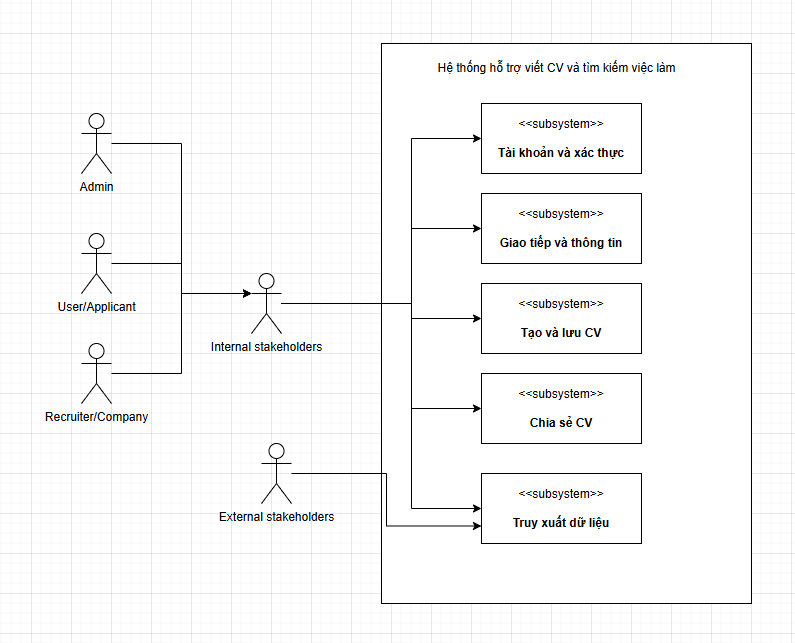
\includegraphics[scale = 0.6]{img/general_usecase.png}
    \caption{Lược đồ usecase chung}
\end{figure}

Hệ thống của trang web hỗ trợ viết CV và tìm kiếm việc làm sẽ chia làm 3 hệ thống nhỏ bao gồm:
\begin{itemize}
    \item \textbf{Hệ thống tài khoản và xác thực:} Thành phần này đảm nhận nhiệm vụ giám sát các tài khoản và xử lý các quy trình xác thực tài khoản.
    \item \textbf{Hệ thống giao tiếp và quản lý thông tin:} Thành phần này chịu trách nhiệm quản lý các tin nhắn và các thông tin của người dùng, CV.
    \item \textbf{Hệ thống truy xuất dữ liệu:} Đây là thành phần đảm nhiệm phần truy xuất dữ liệu của hệ thống và hiển thị lên trang web.
\end{itemize}



\subsubsection{Hệ thống tài khoản và xác thực}

\begin{figure}[H]
	\centering
    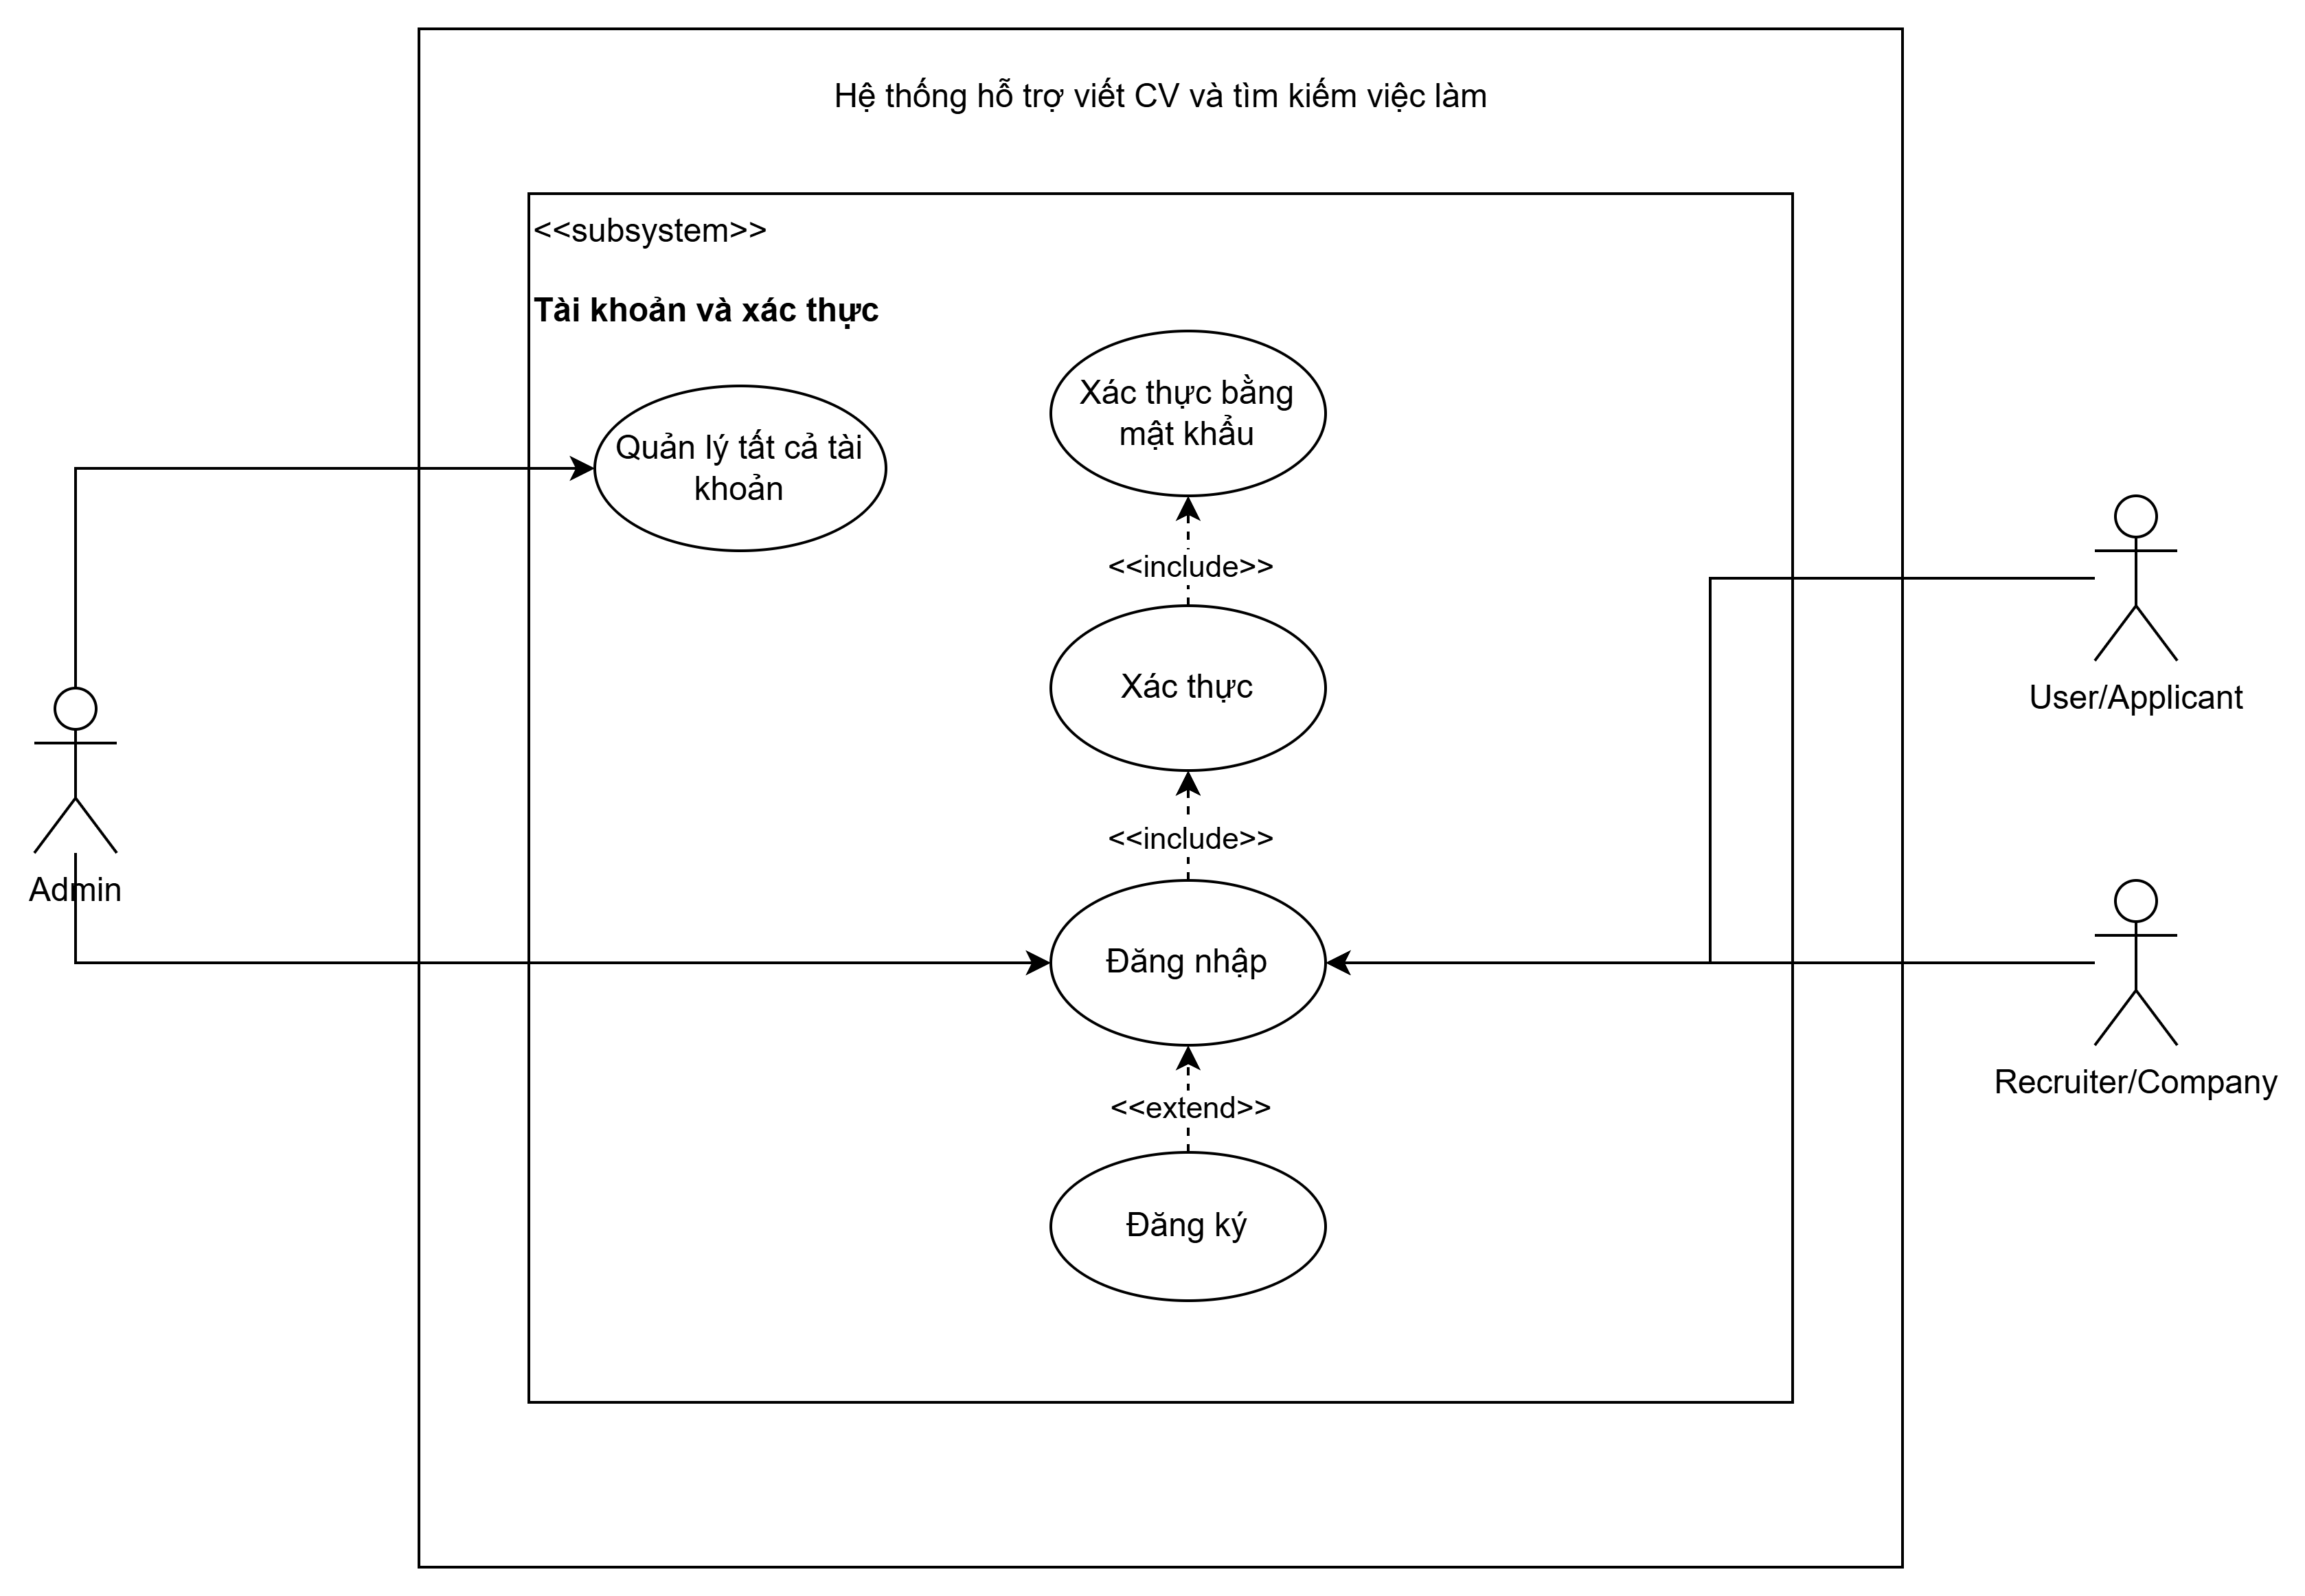
\includegraphics[scale=0.1]{img/AccountAuthenticationUsecase.png}
    \caption{Lược đồ usecase về Hệ thống tài khoản và xác thực}
\end{figure}

Hệ thống con này sẽ chịu trách nhiệm cho việc quản lý tài khoản, mật khẩu của người dùng và quản lý quá trình xác thực của tài khoản, bao gồm việc đăng ký và đăng nhập của tài khoản. Hệ thống sẽ xác thực tài khoản thông qua kiểm tra mật khẩu đã được lưu giữ trước đó ở trong dữ liệu khi lúc đăng ký tạo tài khoản.


\subsubsection{Hệ thống giao tiếp và quản lý thông tin}

\begin{figure}[H]
	\centering
    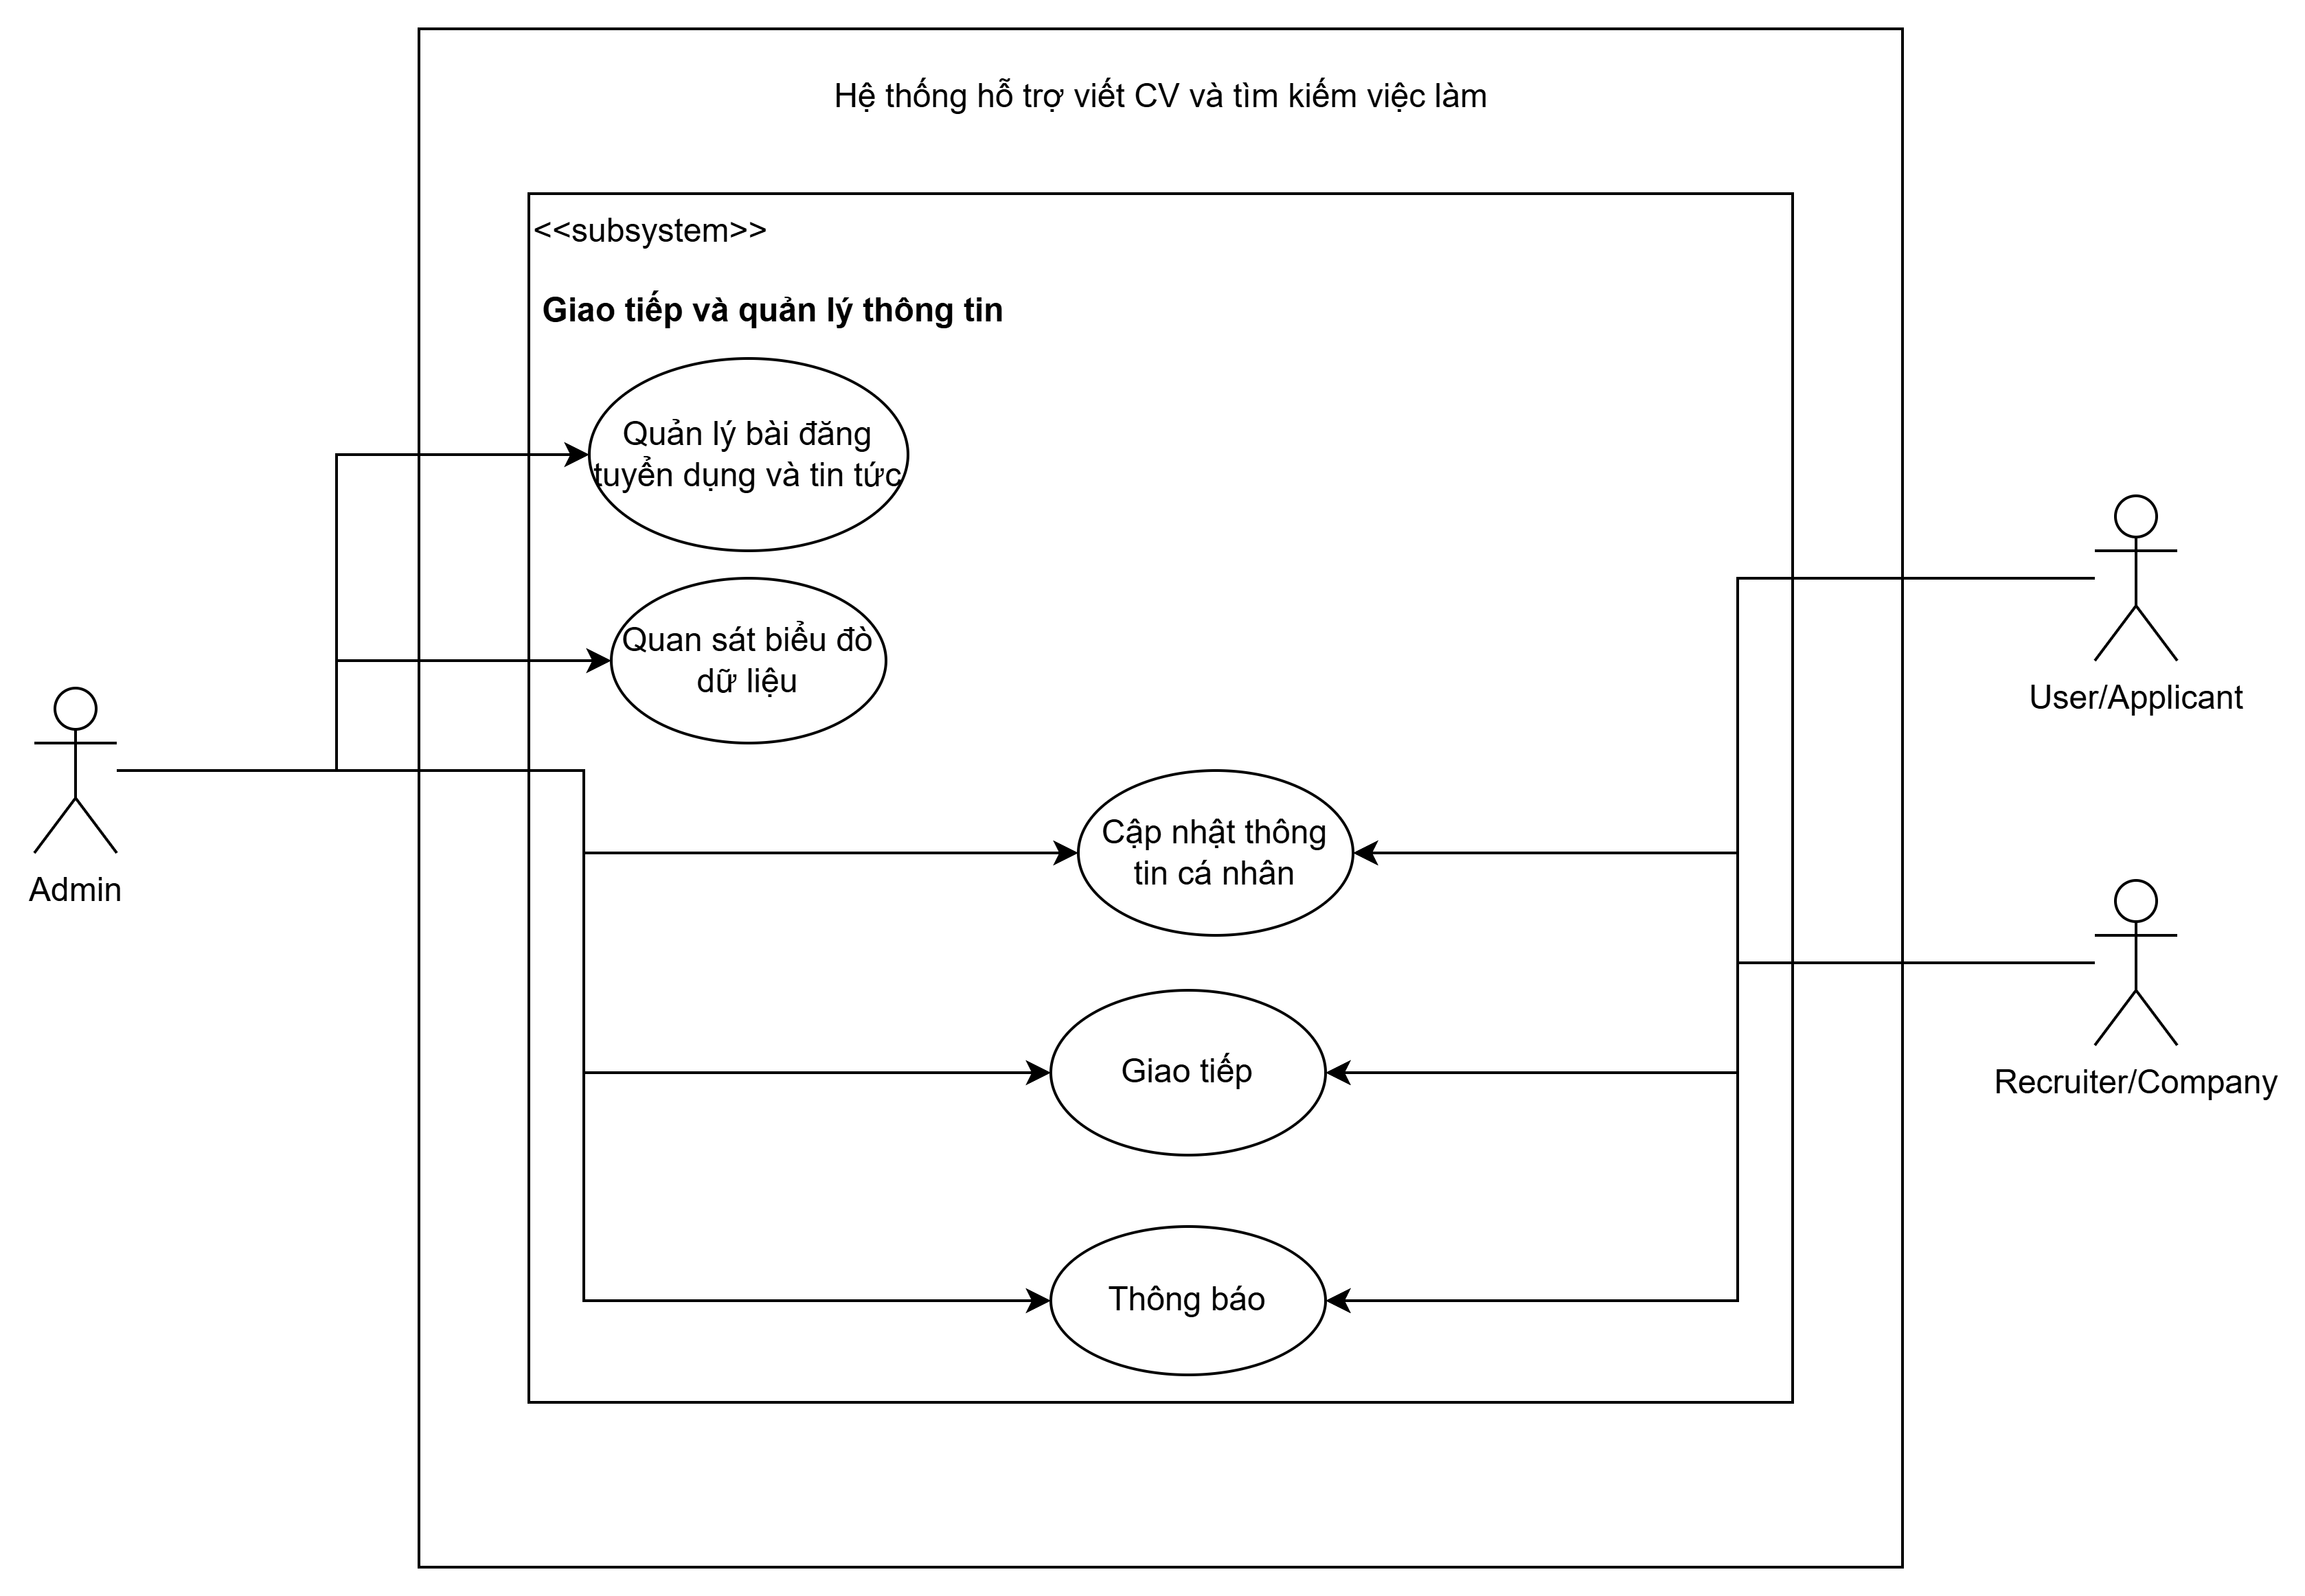
\includegraphics[scale=0.1]{img/communicateInfomationUsecase.png}
    \caption{Lược đồ usecase về Hệ thống giao tiếp và quản lý thông tin}
\end{figure}

Hệ thống sẽ đảm nhiệm vai trò trong việc lưu trữ và truyền tải tin nhắn giữa người với người. Đồng thời, hệ thống này cũng sẽ chịu trách nhiệm trong việc quản lý thông tin người dùng, trong việc chỉnh sửa và cập nhật thông tin cá nhân người dùng.

Đối với admin, hệ thống sẽ chuyển đổi toàn bộ dữ liệu thành bảng biểu, thông số giúp admin có thể dễ dàng tìm hiểu được tình trạng hiện tại của trang web. Admin cũng quản lý những bài đăng, tin tức sẽ xuất hiện trên trang web.


\subsubsection{Hệ thống truy xuất dữ liệu}

\begin{figure}[H]
	\centering
    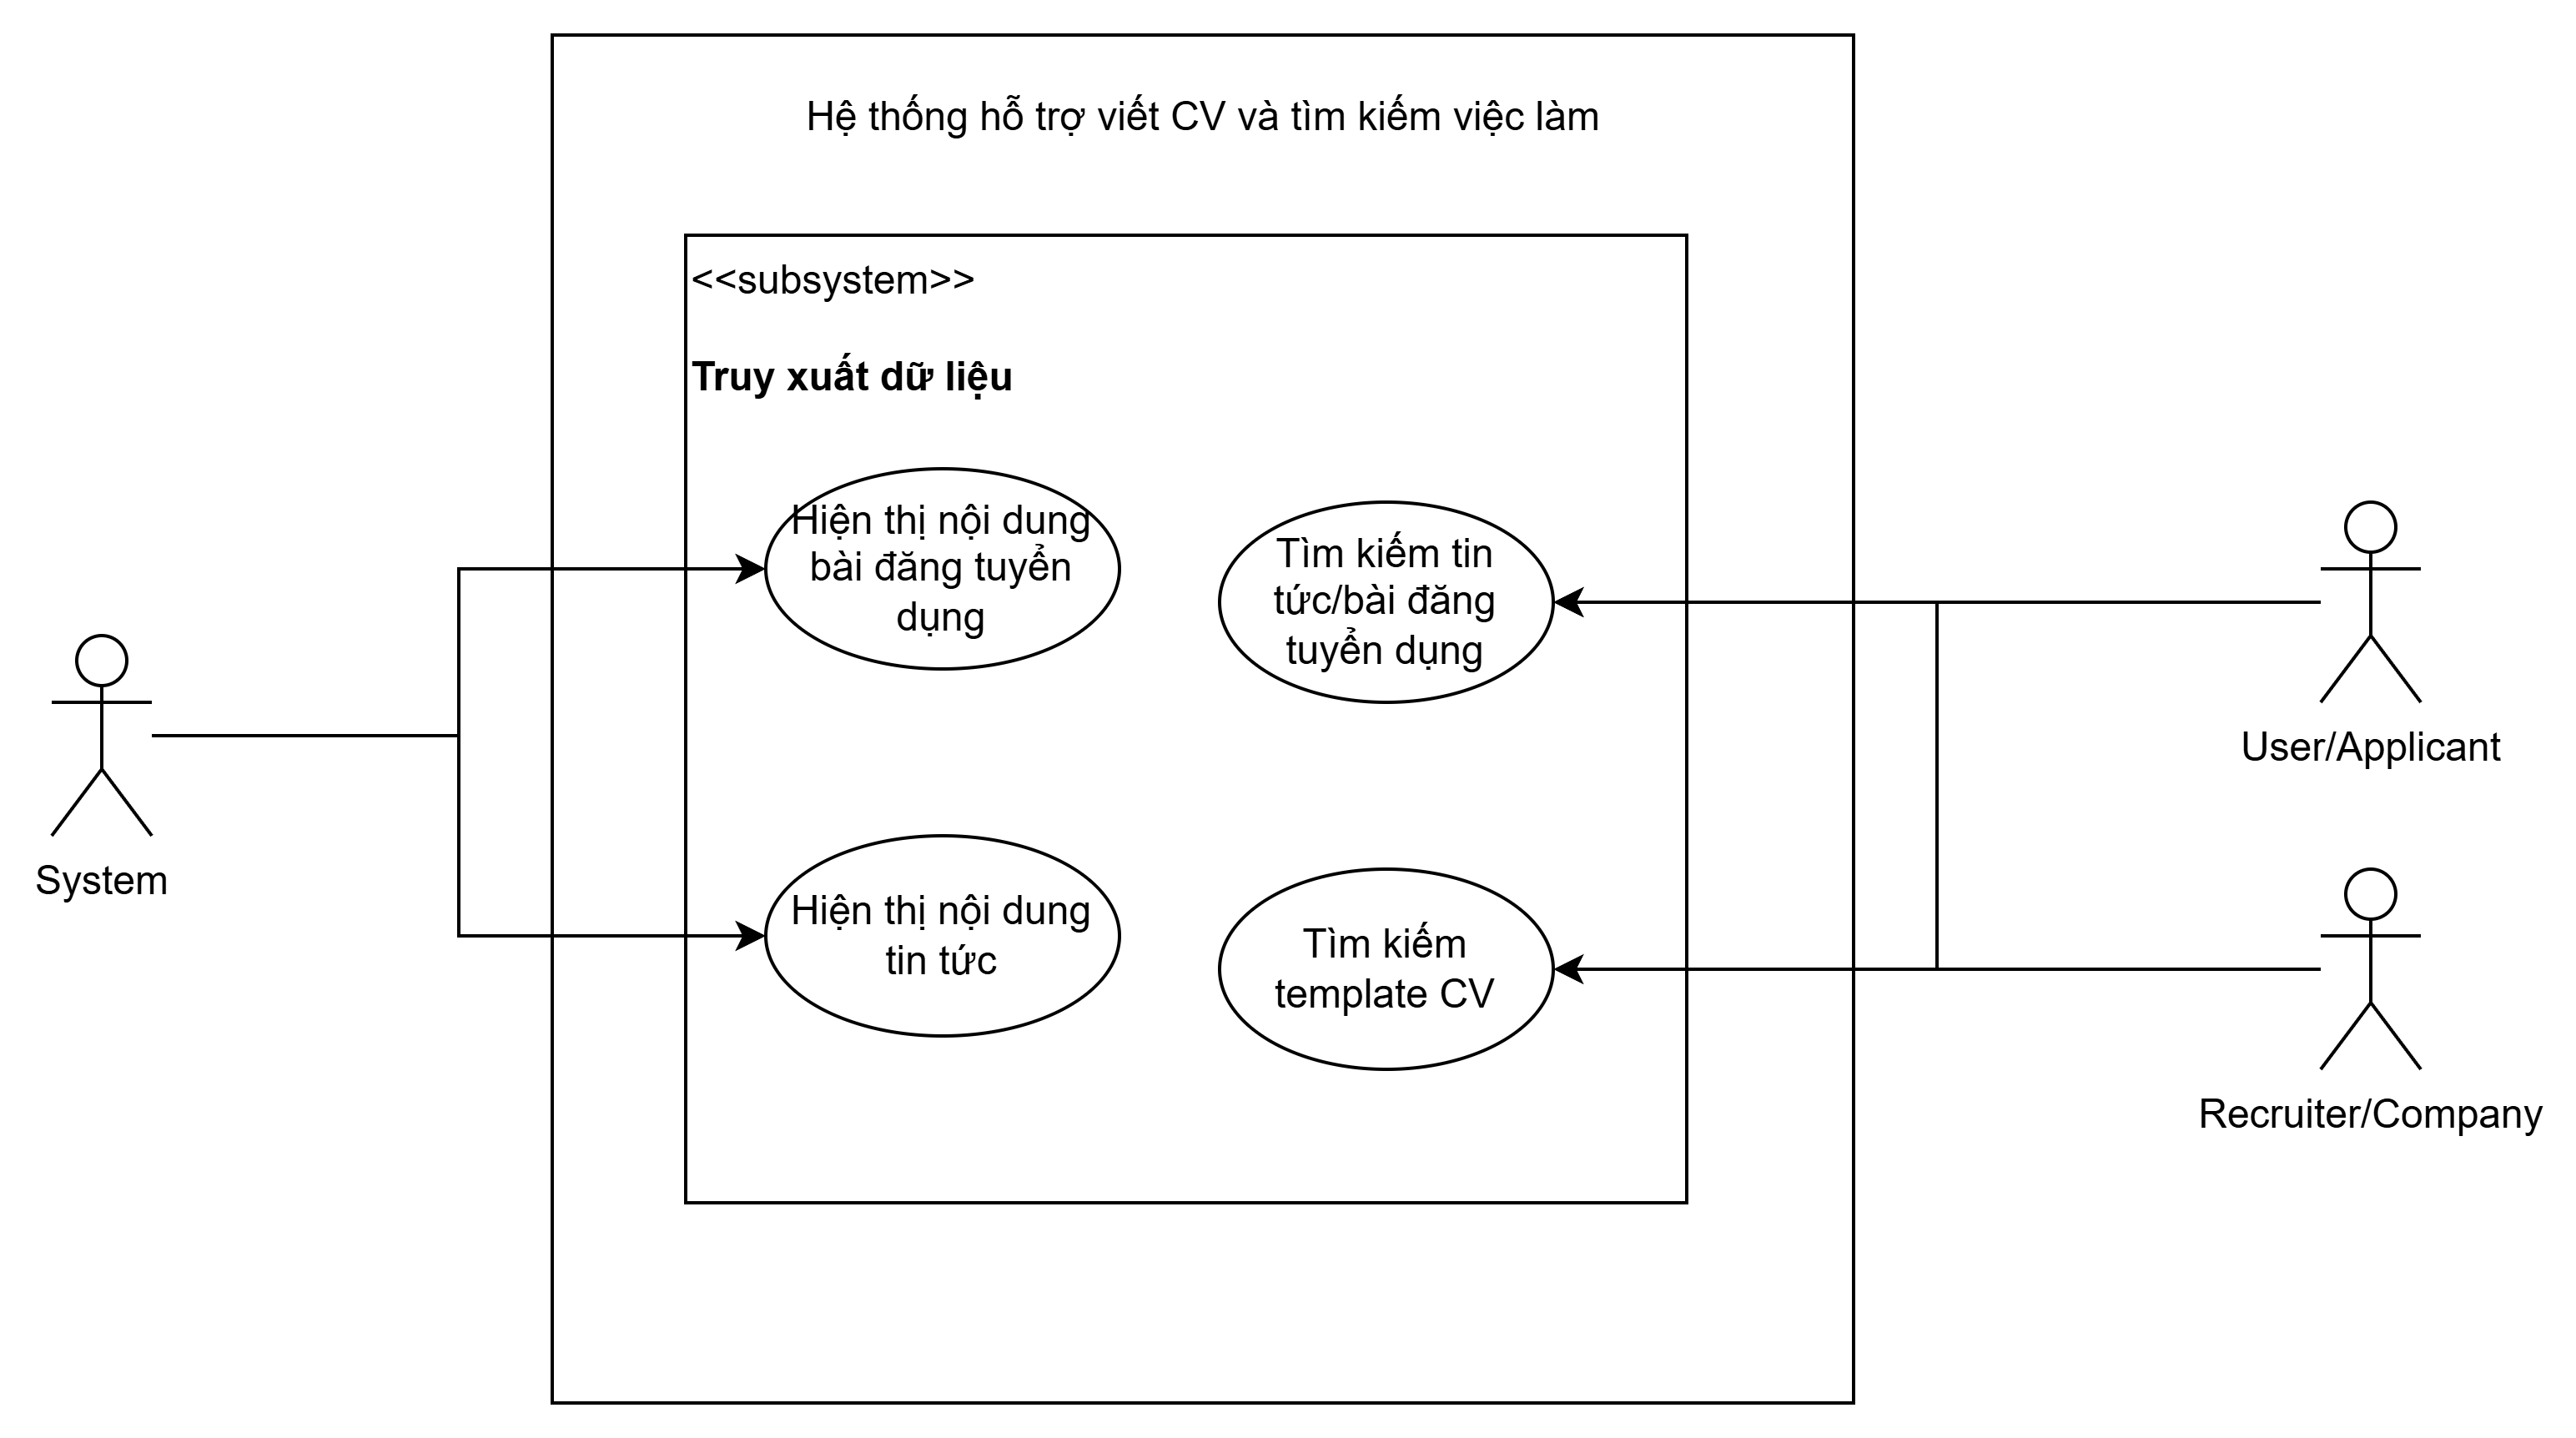
\includegraphics[scale=0.1]{img/TruyXuatDuLieu_Usecase.png}
    \caption{Lược đồ usecase về Hệ thống truy xuất dữ liệu}
\end{figure}

Đây là hệ thống truy xuất dữ liệu. Nơi mà sẽ chịu trách nhiệm cho hiển thị các nội dung có trong trang web như: các bài đăng tuyển dụng, tin tức, CV,.... Đối với người dùng, khi tìm kiếm tin tức hoặc bài đăng tuyển dụng nào hay bất kể template của CV nào, hệ thống sẽ cho hiển thị các nội dung tương ứng lên trang web.

\subsubsection{Lược đồ Usecase tổng quát }
\begin{figure}[H]

	\centering
     \includegraphics[scale = 0.05]{img/overview_usecase.png}
    \caption{Lược đồ usecase tổng quát}
\end{figure}

\url{https://drive.google.com/file/d/1gkpz6ht6IELJw3Rjp8x4X7RPldDnRzsi/view?usp=sharing}


Đây là lược đồ usecase tổng quát của hệ thống trang web hỗ trợ viết CV và tìm kiếm việc làm. Nó thể hiện các chức năng, tác vụ của người dùng, admin và nhà tuyển dụng. Hệ thống này sẽ bao gồm các hệ thống con kể trên nhưng sẽ không chi tiết như vậy. Lược đồ này sẽ mô tả sơ qua các chức năng chính của các bên liên quan chính (internal stakeholders). 

\subsection{Đặc tả lược đồ usecase}


\subsubsection{Đăng ký tài khoản (sử dụng mật khẩu)}


\begin{table}[H]
    \centering
    \begin{tabular}{|>{\centering\arraybackslash}p{0.3\linewidth}|>{\raggedright\arraybackslash}p{0.7\linewidth}|} \hline 
         ID& 1\\ \hline 
         Tên lược đồ usecase& Đăng ký tài khoản\\ \hline 
         Actors& User (Applicant)\\ \hline 
         Mô tả& Người dùng tạo một tài khoản mới ở đây\\ \hline 
         Tiền điều kiện (Pre-conditions)& Người dùng chưa có tài khoản.
Người dùng đang ở trang đăng ký tạo tài khoản mới.\\ \hline 
 Hậu điều kiện (Post-conditions)&Người tạo tài khoản mới thành công.\\\hline 
         Luồng thực thi chính (Normal flow)& 1. Người dùng vào trang tạo tài khoản mới.

2. Trang web sẽ hiện thị nội dung cần phải điền khi tạo tài khoản.

3. Người dùng điền thông tin vào.

4. Hệ thống kiểm tra liệu tài khoản đã có hay chưa.

5. Nếu tài khoản chưa có, thì thông báo tài khoản của người dùng được tạo thành công.\\ \hline 
         Luồng thực thi thay thế (Alternative flow)& \\ \hline 
         Luồng thực thi ngoại lệ (Exception flow)& 5.1.1. Ở bước thứ 5 nếu hệ thống kiểm tra tài khoản đã có rồi thì hệ thống sẽ hiển thị thông báo "Tài khoản đã có người dùng khác sử dụng".

5.1.2. Người dùng đổi lại tên tài khoản. Sau đó quay trở lại bước 4.\\ \hline
    \end{tabular}
    \caption{Bảng đặc tả usecase cho Đăng ký tài khoản}
    \label{tab:Register}
\end{table}



\subsubsection{Đăng nhập tài khoản}


\begin{table}[H]
    \centering
    \begin{tabular}{|>{\centering\arraybackslash}p{0.3\linewidth}|>{\raggedright\arraybackslash}p{0.7\linewidth}|} \hline 
         ID
& 2\\ \hline 
         Tên lược đồ usecase
& Đăng nhập tài khoản bằng mật khẩu\\ \hline 
         Actors
& Admin, user, company/recruiter\\ \hline 
         Mô tả
& Người dùng cố gắng đăng nhập vào hệ thống.\\ \hline 
         Tiền điều kiện (Pre-conditions)
& Người dùng đã có tài khoản hoặc đã tạo tài khoản trước đó.
Người dùng đang ở trang đăng nhập.\\ \hline 
         Hậu điều kiện (Post-conditions)
& Người dùng đăng nhập vô hệ thống thành công.\\ \hline 
         Luồng thực thi chính (Normal flow)
& 1. Người dùng vào trang đăng nhập.

2. Hệ thống hiển thị trang đăng nhập.

3. Người dùng điền tài khoản và mật khẩu vào trang web.

4. Hệ thống kiểm tra thông tin tài khoản và mật khẩu của người dùng liệu có khớp với dữ liệu được lưu trữ hay không.

5. Nếu khớp, hệ thống chuyển trang cho người dùng đến trang chủ của trang web và thông báo "Người dùng đã đăng nhập thành công.".\\ \hline 
         Luồng thực thi thay thế (Alternative flow)
& \\ \hline
 Luồng thực thi ngoại lệ (Exception flow)&5.1.1. Nếu hệ thống kiểm tra thông tin tài khoản và mật khẩu của người dùng không khớp thì người dùng sẽ được đưa về lại trang đăng nhập và được thông báo rằng "Tài khoản/Mật khẩu của người dùng không đúng."

5.1.2. Người dùng điền lại thông tin tài khoản và mật khẩu và quay lại bước 4.\\\hline
    \end{tabular}
    \caption{Bảng đặc tả usecase cho Đăng nhập tài khoản}
    \label{tab:Đăng nhập tài khoản}
\end{table}


\subsubsection{Tìm kiếm và chọn CV Template}

\begin{table}[H]
    \centering
    \begin{tabular}{|>{\centering\arraybackslash}p{0.3\linewidth}|>{\raggedright\arraybackslash}p{0.7\linewidth}|} \hline 
         ID
& 3\\ \hline 
         
Tên lược đồ usecase
& Tìm kiếm và chọn lựa template CV\\ \hline 
         Actors
& User\\ \hline 
         
Mô tả
& Người dùng tìm kiếm và chọn lựa các template của CV dựa trên CV có sẵn trên hệ thống.\\ \hline 
         Tiền điều kiện (Pre-conditions)
& Người đăng nhập vào tài khoản thành công\\ \hline 
         
Hậu điều kiện (Post-conditions)& Người dùng chọn lựa template CV thành công\\ \hline 
         Luồng thực thi chính (Normal flow)& 1. Người dùng vào trang CV của mình và chọn mục Template

2. Người dùng tìm kiếm và chọn cho mình template CV thích hợp với mình.

3. Sau đó người dùng đặt tên cho CV của mình và điền vào CV những thông tin mà CV yêu cầu theo từng ô được chỉ định.

4. Người dùng lưu lại CV. Nếu lưu lại CV thành công, hệ thống sẽ thông báo cho người dùng "Lưu CV thành công"\\ \hline 
         
Luồng thực thi thay thế (Alternative flow)
& Ở bước 2, nếu người dùng không tìm được CV ưng ý với mình. Người dùng có thể chọn mục Custom. Ở đây, người dùng có thể tự mình thiết kế CV phù hợp với mình nhất.\\ \hline
 Luồng thực thi ngoại lệ (Exception flow)&4.1 Nếu hệ thống lưu CV không thành công (do bởi kết nối mạng), hệ thống sẽ thông báo cho người dùng rằng: "Lưu CV thất bại do sự cố kết nối."\\\hline
    \end{tabular}
    \caption{Bảng đặc tả usecase cho Tìm kiếm và chọn lựa CV Template}
    \label{tab:Tìm kiếm và chọn CV templates}
\end{table}



\subsubsection{Quản lý CV}

\begin{table}[H]
    \centering
    \begin{tabular}{|>{\centering\arraybackslash}p{0.3\linewidth}|>{\raggedright\arraybackslash}p{0.7\linewidth}|} \hline 
         ID
& 4\\ \hline 
         
Tên lược đồ usecase
& Quản lý CV\\ \hline 
         Actors
& User\\ \hline 
         
Mô tả
& Người dùng quản lý (thêm, xoá, sửa) CV của mình.\\ \hline 
         Tiền điều kiện (Pre-conditions)
& Người dùng đã tạo tài khoản thành công.\\ \hline 
         
Hậu điều kiện (Post-conditions)& Người dùng có thể quản lý CV của mình.\\ \hline 
         Luồng thực thi chính (Normal flow)& 1. Người dùng vào trang "CV của mình".

2. Người dùng chọn 1 bản CV để chỉnh sửa hoặc xoá.

3. Nếu người dùng chọn sửa, hệ thống sẽ đưa người dùng đến trang chỉnh sửa CV và người dùng sẽ dựa vào những công cụ mà trang web có mà chỉnh sửa.

4. Hệ thống lưu lại những sự thay đổi đối với CV bạn đã chọn\\ \hline 
         
Luồng thực thi thay thế (Alternative flow)
& 3.1. Nếu người dùng chọn xoá CV thì hệ thống sẽ xoá dữ liệu của bản CV đó ra khỏi hệ thống dữ liệu. Và hệ thống sẽ reload lại trang với những dữ liệu mới được cập nhật.\\ \hline
 Luồng thực thi ngoại lệ (Exception flow)&4.1. Nếu không có kết nối mạng hoặc lỗi kết nối, dữ liệu sẽ không được lưu.\\\hline
    \end{tabular}
    \caption{Bảng đặc tả usecase cho Quản lý CV}
    \label{tab: Quản lý CV}
\end{table}



\subsubsection{Tìm kiếm bài đăng tuyển dụng}

\begin{table}[H]
    \centering
    \begin{tabular}{|>{\centering\arraybackslash}p{0.3\linewidth}|>{\raggedright\arraybackslash}p{0.7\linewidth}|} \hline 
         ID
& 5\\ \hline 
         
Tên lược đồ usecase
& Tìm kiếm bài đăng tuyển dụng\\ \hline 
         Actors
& Users, recuiter, external stakeholders\\ \hline 
         
Mô tả
& Người dùng tìm kiếm bài đăng tuyển dụng từ các công ty.\\ \hline 
         Tiền điều kiện (Pre-conditions)
& \\ \hline 
         
Hậu điều kiện (Post-conditions)& Người dùng có thể tìm kiếm công việc dễ dàng và hợp ý mình.\\ \hline 
         Luồng thực thi chính (Normal flow)& 1. Người dùng vào trang "Tìm việc làm".

2. Hệ thống hiển thị trang "Tìm việc làm" và liệt kê các bài đăng tuyển dụng công việc hiện có.

3. Chọn thanh tìm kiếm trên trang web.

4. Điền tên công việc mà bản thân muốn tìm kiếm.

5. Hệ thống tìm kiếm từ dữ liệu những bài đăng tuyển dụng trùng tên với tên công việc đang tìm kiếm.

6. Sau khi tìm kiếm, hệ thống sẽ liệt kê ra trang web những bài đăng tuyển dụng. Người dùng có thể chọn các loại filter, sort theo ngày, giờ, địa điểm.\\ \hline 
         
Luồng thực thi thay thế (Alternative flow)
& \\ \hline
 Luồng thực thi ngoại lệ (Exception flow)&6.1. Nếu hệ thống không tìm thấy dữ liệu trùng với tên công việc mà mình đang tìm kiếm, hệ thống sẽ thông báo "Không tìm thấy thông tin trùng với tên bạn tìm kiếm".\\\hline
    \end{tabular}
    \caption{Bảng đặc tả usecase cho Tìm kiếm bài đăng tuyển dụng}
    \label{tab:Tìm kiếm bài đăng tuyển dụng}
\end{table}

\subsubsection{Ứng tuyển công việc}

\begin{table}[H]
    \centering
    \begin{tabular}{|>{\centering\arraybackslash}p{0.3\linewidth}|>{\raggedright\arraybackslash}p{0.7\linewidth}|} \hline 
         ID
& 6\\ \hline 
         
Tên lược đồ usecase
& Ứng tuyển công việc\\ \hline 
         Actors
& User\\ \hline 
         
Mô tả
& Người dùng ứng tuyển vào vị trí của bài đăng tuyển dụng.\\ \hline 
         Tiền điều kiện (Pre-conditions)
& Người đã tạo tài khoản thành công.

Người dùng đã có CV đầy đủ cho chính mình trên web hoặc upload CV có sẵn của bản thân mình.\\ \hline 
         
Hậu điều kiện (Post-conditions)& \\ \hline 
         Luồng thực thi chính (Normal flow)& 1. Người dùng chọn 1 bài đăng tuyển dụng phù hợp với mình.

2. Hệ thống sẽ hiển thị những thông tin chi tiết liên quan đến bài đăng tuyển dụng.

3. Người dùng chọn "Ứng tuyền" ở bên trong bài viết.

4. Nếu người đã có CV đầy đủ, hệ thống sẽ thông báo cho người dùng "Ứng tuyển thành công".\\ \hline 
         
Luồng thực thi thay thế (Alternative flow)
& \\ \hline
 Luồng thực thi ngoại lệ (Exception flow)&4.1. Nếu người dùng chưa có CV đầy đủ hoặc chưa upload CV của riêng mình thì hệ thống sẽ thông báo cho người dùng "Ứng tuyển thất bại" và di chuyển người dùng đến trang "Quản lý CV" của mình.\\\hline
    \end{tabular}
    \caption{Bảng đặc tả usecase cho Ứng tuyển công việc}
    \label{tab:Ứng tuyển công việc}
\end{table}

\subsubsection{Chia sẻ CV}

\begin{table}[H]
    \centering
    \begin{tabular}{|>{\centering\arraybackslash}p{0.3\linewidth}|>{\raggedright\arraybackslash}p{0.7\linewidth}|} \hline 
         ID
& 7\\ \hline 
         
Tên lược đồ usecase
& Chia sẻ CV\\ \hline 
         Actors
& User\\ \hline 
         
Mô tả
& Người dùng chia sẻ CV của mình đến những người dùng khác hoặc chia sẻ CV của mình đến các nhà tuyển dụng để họ tìm đến mình.\\ \hline 
         Tiền điều kiện (Pre-conditions)
& Người dùng tạo tài khoản thành công.

Người dùng đã có CV hoàn chỉnh hoặc upload CV của riêng mình.\\ \hline 
         
Hậu điều kiện (Post-conditions)& Người dùng chia sẻ CV đến mọi người thành công.\\ \hline 
         Luồng thực thi chính (Normal flow)& 1. Người dùng vào trang "Quản lý CV" của mình.

2. Người dùng chọn một CV mà mình ưng ý và muốn chia sẻ chúng.

3. Người dùng vào trang CV đó và ở góc phải, người chọn "Chia sẻ".

4. Hệ thống hiển thị ra 2 option cho người dùng chọn: "Chia sẻ đến người dùng khác" và "Chia sẻ tìm kiếm công việc".

5. Người dùng chọn 1 trong 2 option hoặc cả 2.

6. Nếu thành công, hệ thống thông báo đến người dùng "Chia sẻ thành công".\\ \hline 
         
Luồng thực thi thay thế (Alternative flow)
& 6.1. Nếu người dùng chọn option "Chia sẻ đến người dùng khác", sau khi chia sẻ thành công, người dùng có thể copy link CV của mình và gửi đến những người dùng khác.\\ \hline
 Luồng thực thi ngoại lệ (Exception flow)&\\\hline
    \end{tabular}
    \caption{Bảng đặc tả usecase cho Chia sẻ CV}
    \label{tab:Chia sẻ CV}
\end{table}





\section{Thiết kế quy trình làm việc (Workflow design)}


\subsection{Đăng ký tài khoản (Register)}

\begin{figure}[H]

	\centering
    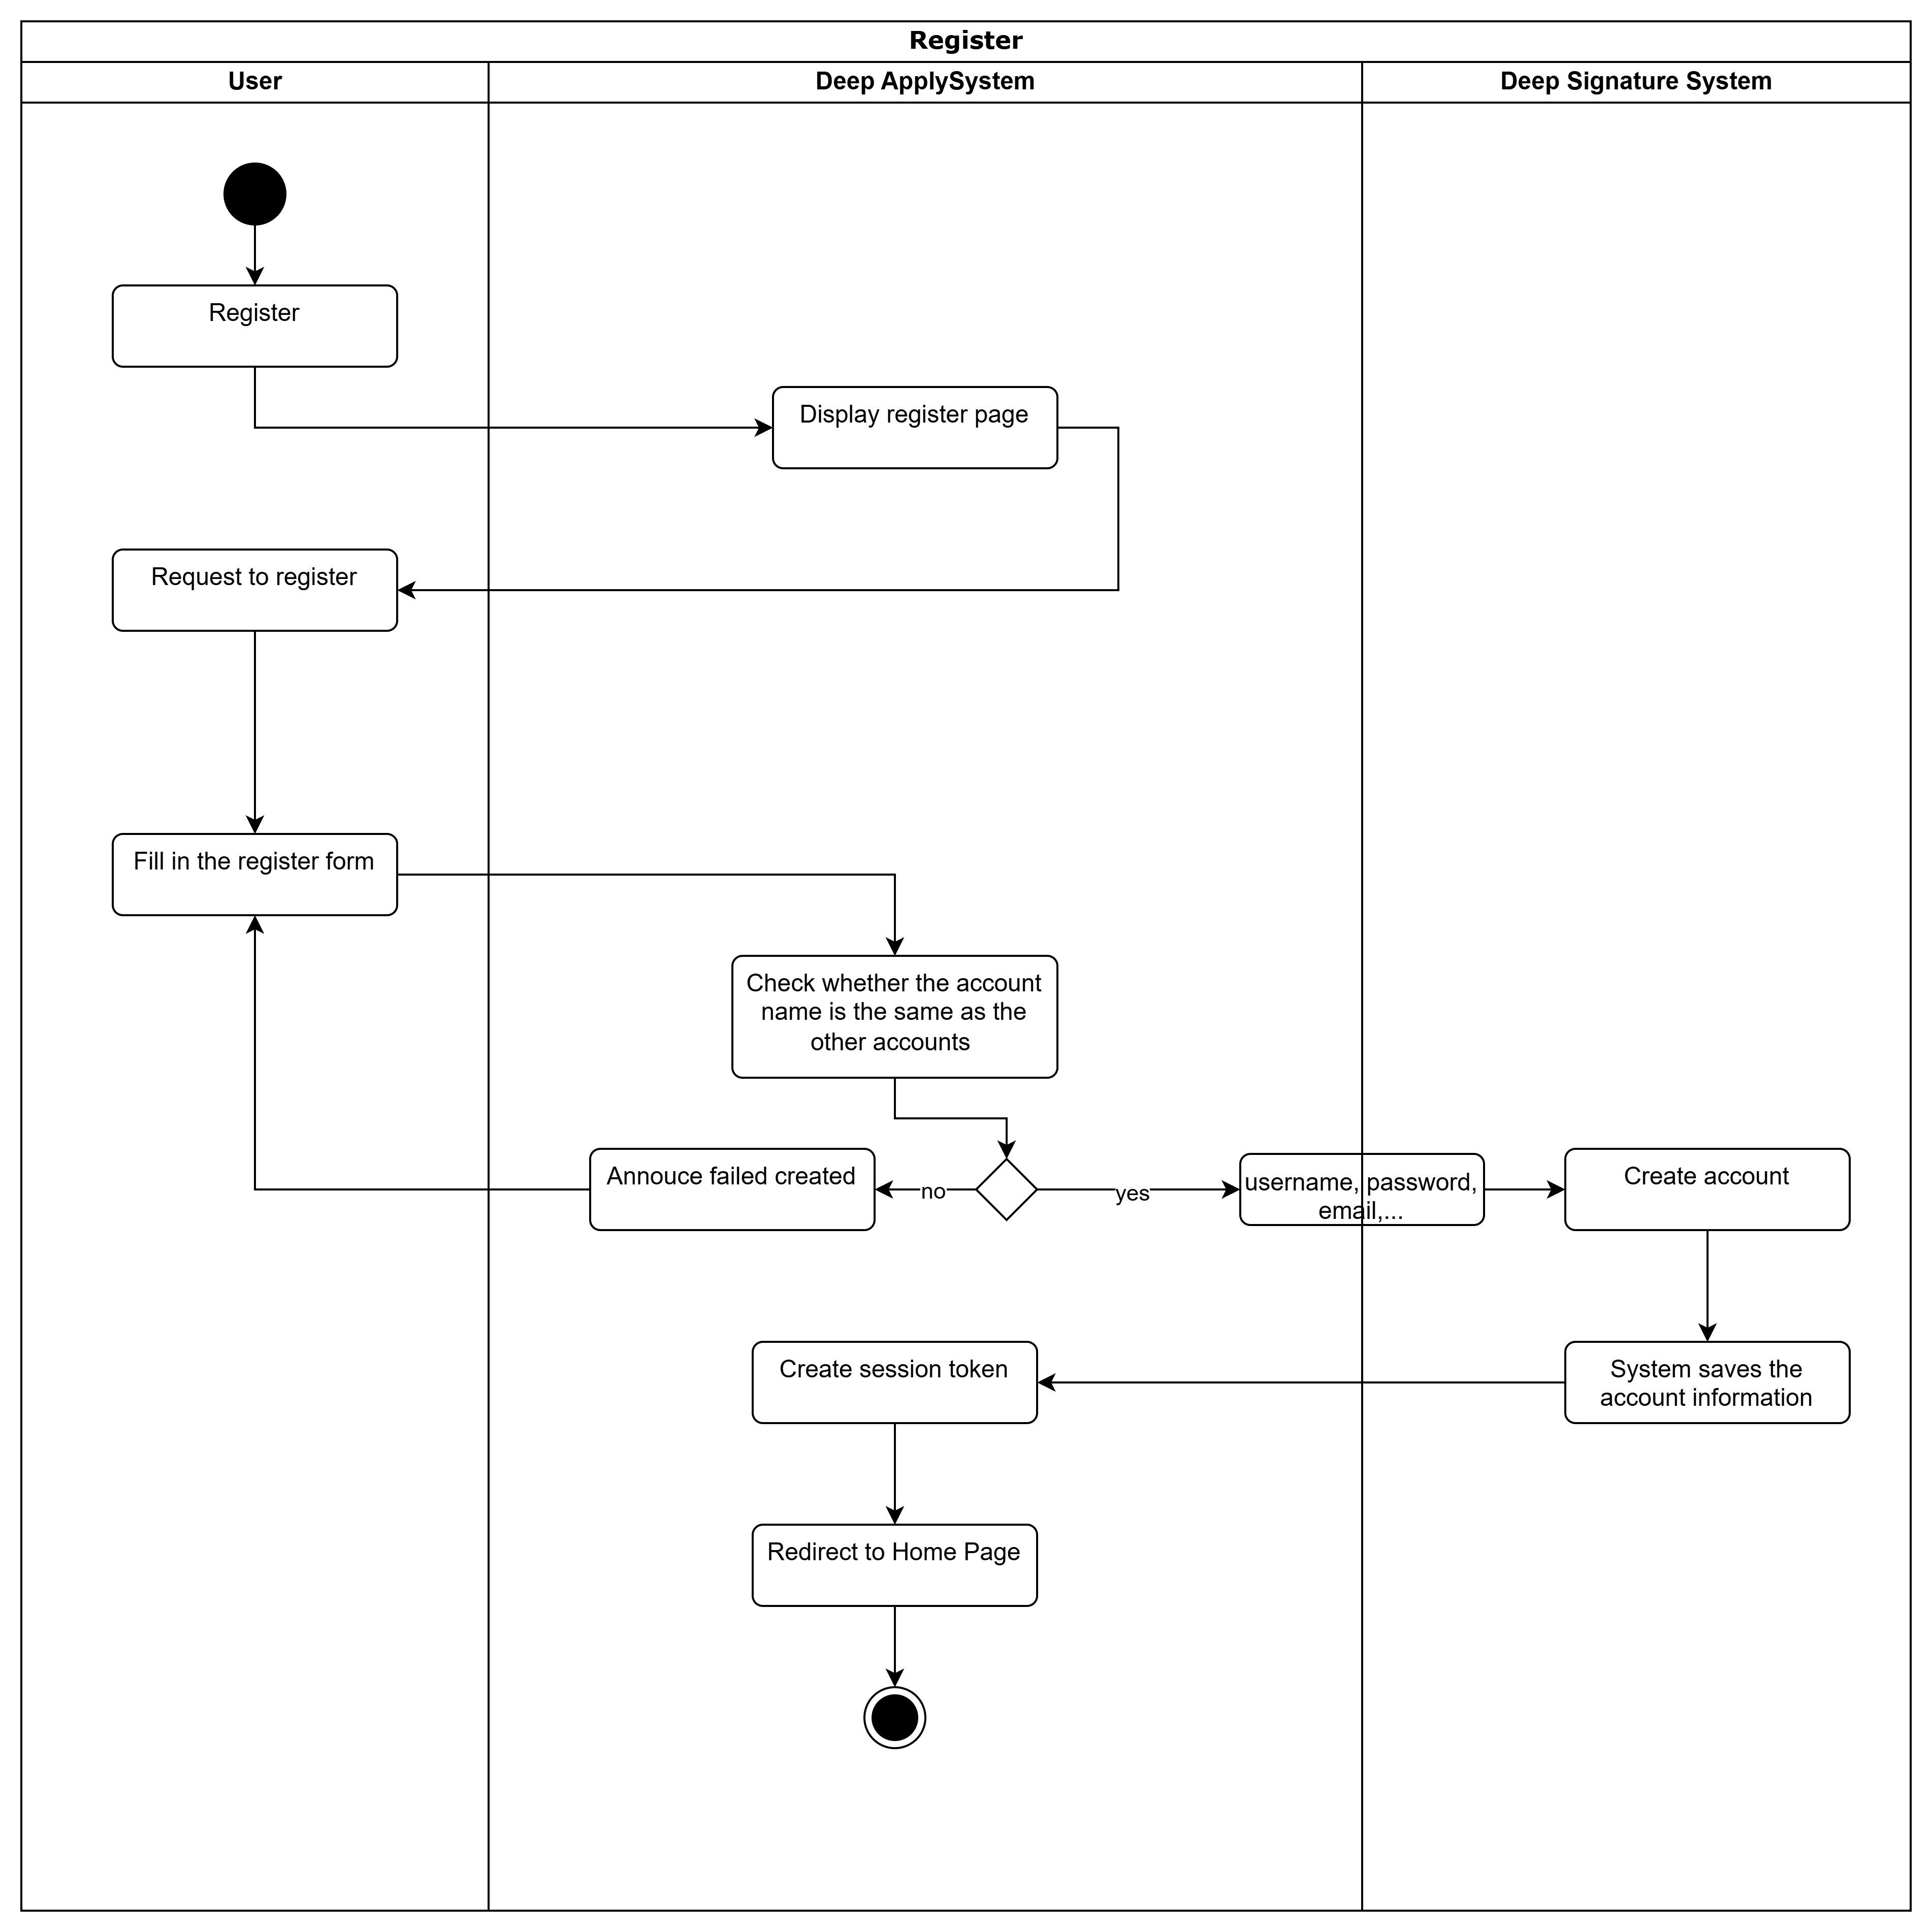
\includegraphics[scale=0.08]{img/Register_workflow.png}
    \caption{Lược đồ hoạt động về Đăng ký tài khoản}

\end{figure}

Biểu đồ trên mô tả quy trình làm việc của quá trình đăng ký tài khoản. Sau khi người dùng bấm vào nút Đăng ký, hệ thống sẽ đưa người dùng đến trang đăng ký tài khoản. Ở đây sẽ có 1 form yêu cầu những thông tin cần thiết của người dùng để có thể tạo tài khoản thành công. Sau khi điền thông tin xong, người dùng bấm vào nút "Đăng ký" bên dưới form. Sau đó hệ thống sẽ bắt đầu kiểm tra thông tin người dùng hợp lệ hay không. Sau khi hệ thống kiểm tra tài khoản của người dùng không bị trùng lặp với những tài khoản khác, người dùng sẽ được hệ thống thông báo tạo tài khoản thành công và chuyển hướng trang đến trang chủ. Còn nếu tài khoản bị trùng lặp, người dùng sẽ bị quay lại ở trang Đăng ký tài khoản và chỉnh sửa lại tên tài khoản sao cho không bị trùng lặp với những người dùng khác. Trong trường hợp người dùng chưa điền hết thông tin cần thiết, hệ thống sẽ hiển thị thông báo cho người dùng "Bạn chưa hoàn thành form thông tin đăng ký tài khoản". Sau khi tạo tài khoản thành công, toàn bộ thông tin người dùng sẽ được lưu trữ vào cơ sở dữ liệu của hệ thống.

\subsection{Đăng nhập tài khoản (Login)}

\begin{figure}[H]

	\centering
    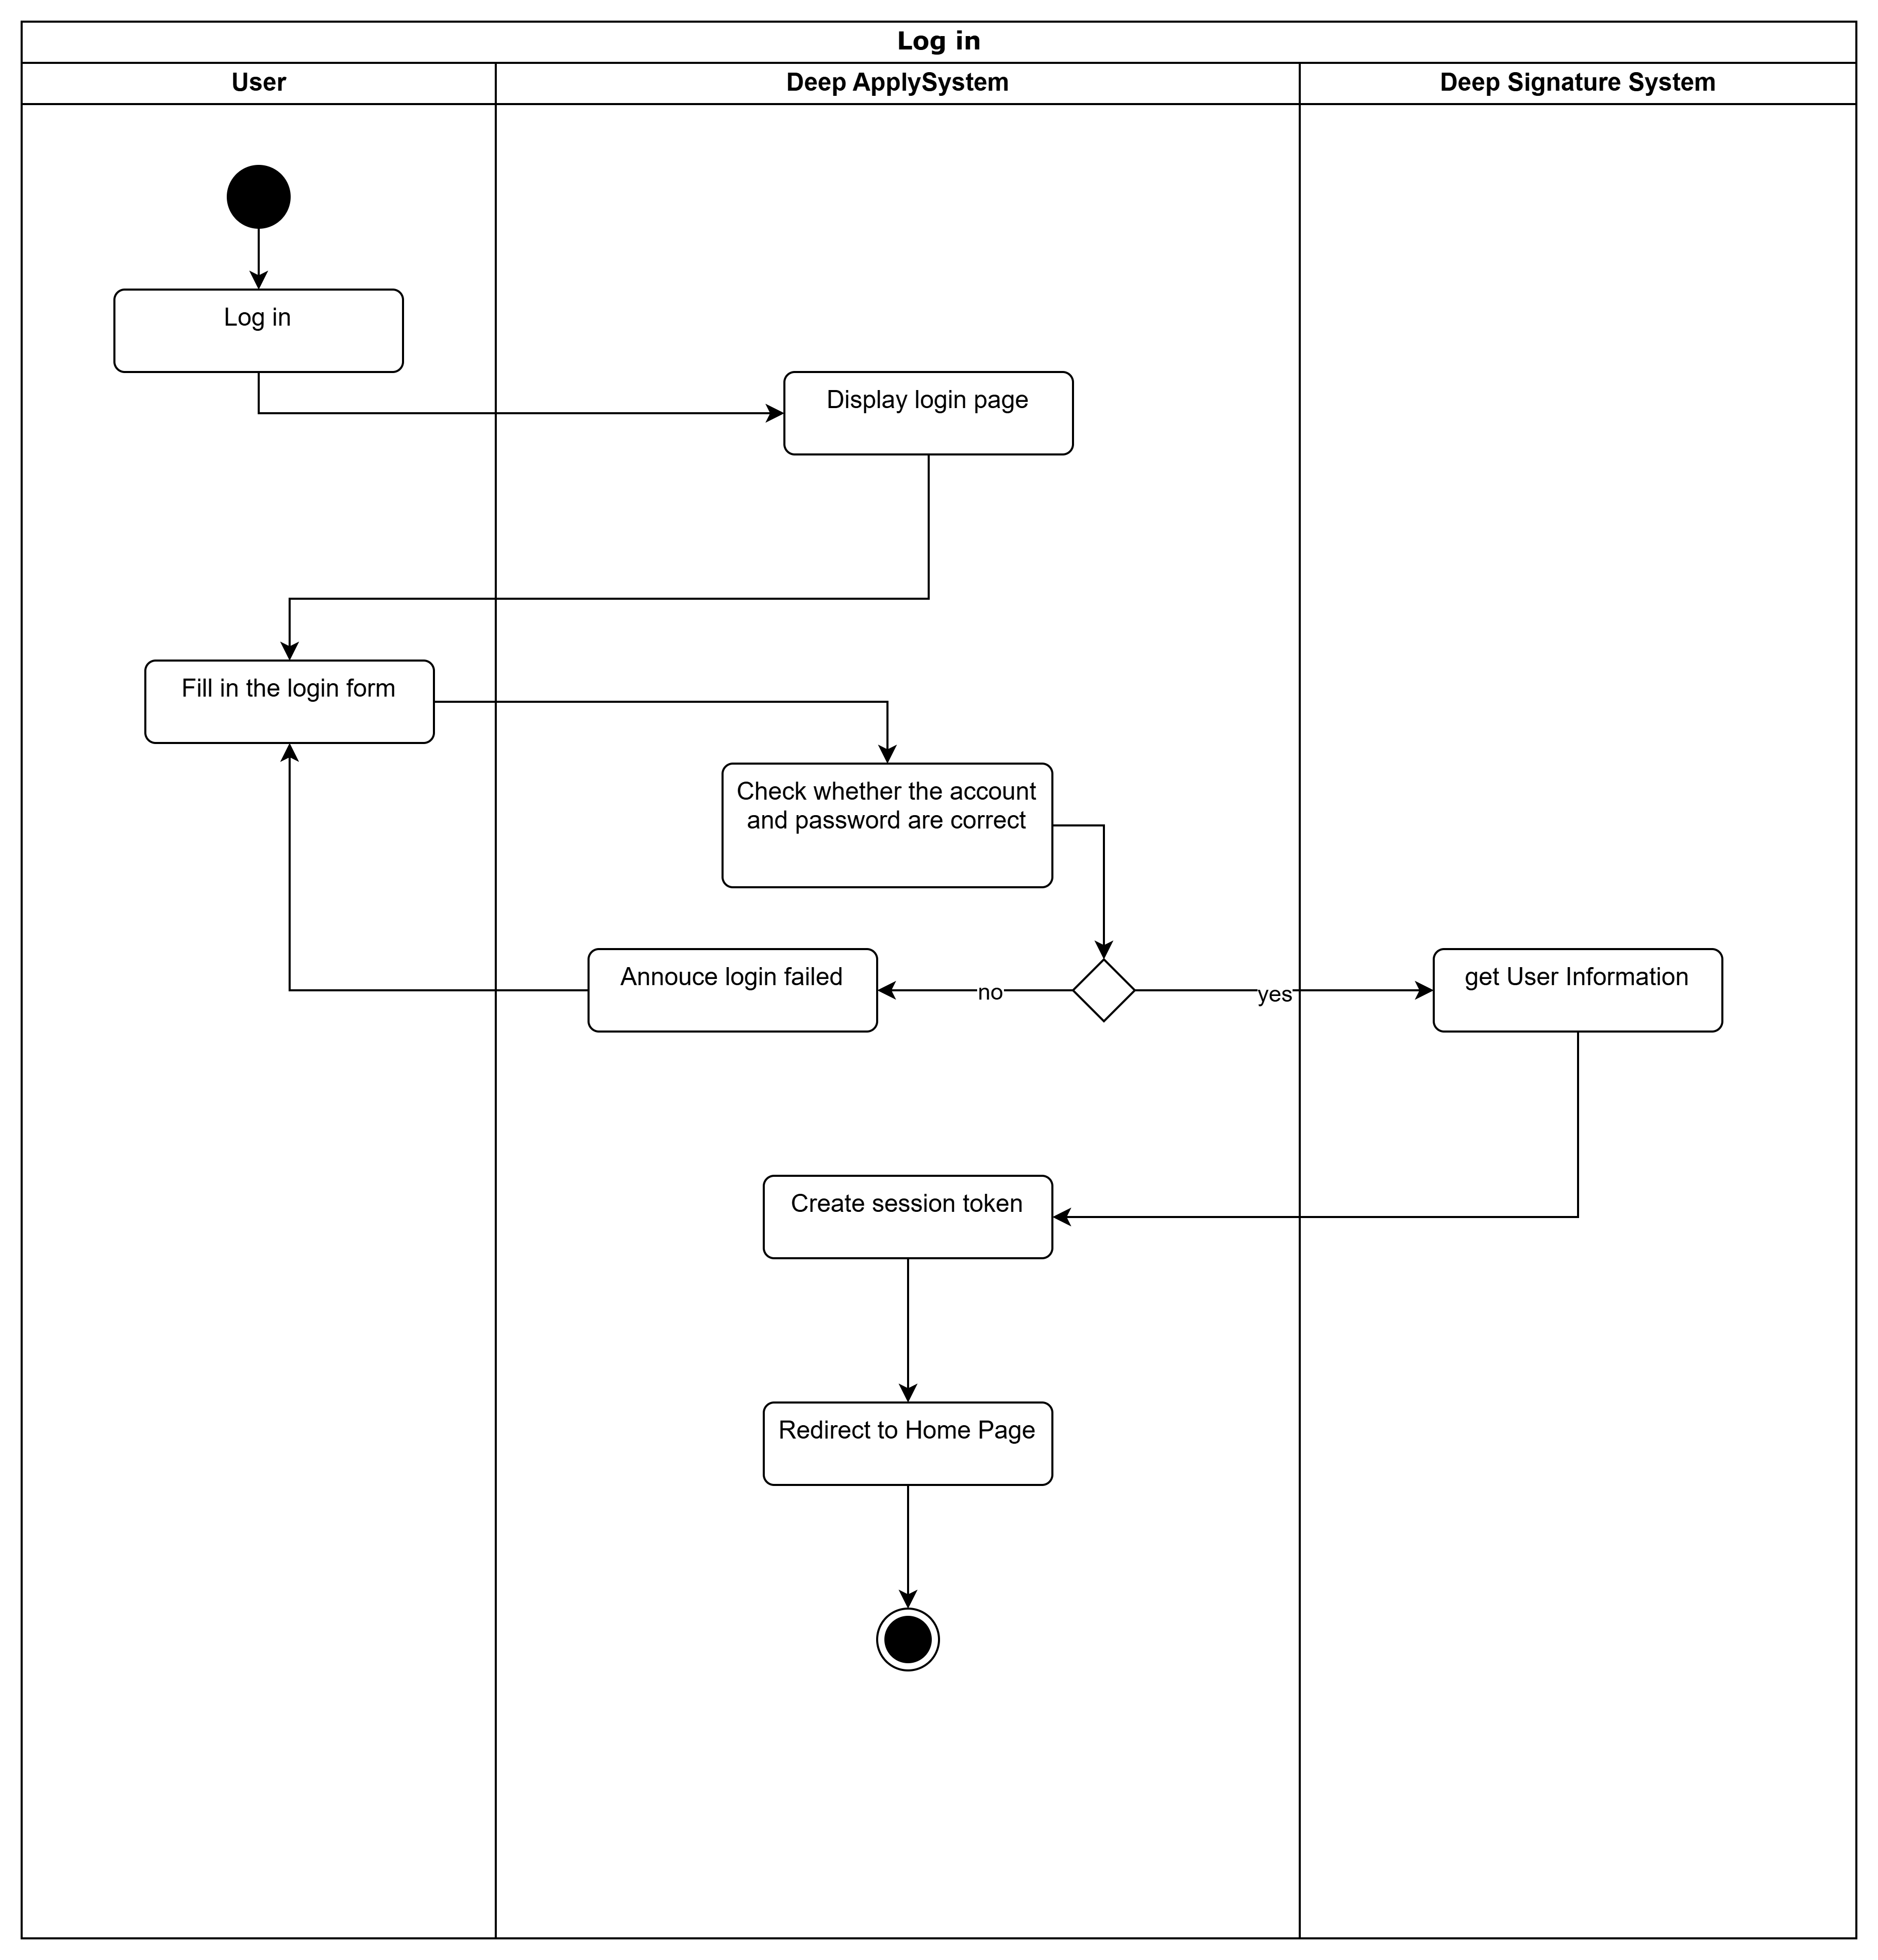
\includegraphics[scale=0.08]{img/Login_workflow.png}
    \caption{Lược đồ hoạt động về Đăng nhập tài khoản}
\end{figure}

Quy trình làm việc cho biểu đồ hoạt động của "Đăng nhập tài khoản": sẽ chia làm 2 đối tượng, một là những người sử dụng bình thường và còn lại là những tài khoản công ty được admin cung cấp để sử dụng. Người dùng lựa chọn 1 trong 2 option là "Người dùng" và "Doanh nghiệp". Sau đó sẽ được hệ thống đưa đến và hiển thị trang "Login page". Sau khi người dùng điền tài khoản và mật khẩu, hệ thống sẽ thực hiện chức năng xác thực, kiểm tra xem liệu người dùng điền thông tin tài khoản và mật khẩu trùng với dữ liệu hệ thống không? Nếu tài khoản và mật khẩu của người dùng trùng với dữ liệu của hệ thống, người dùng sẽ được hệ thống chuyển hướng tới trang "Trang chủ" của trang web.

Nếu tài khoản và mật khẩu của người dùng không khớp với bất kỳ dữ liệu của hệ thống, người dùng sẽ được hiển thị thông báo "Tài khoản hoặc mật khẩu của bạn không chính xác. Vui lòng kiểm tra lại." và bị giữ lại ở trang Đăng nhập. Người cũng có một lựa chọn khác là tạo một tài khoản mới với chức năng "Đăng ký tài khoản.". Quy trình làm việc của chức năng "Đăng ký tài khoản" đã được trình bày ở trên. Sau khi đăng nhập thành công, hệ thống sẽ tạo 1 session token và lưu giữ trên máy tính của người dùng nhằm duy trì trạng thái đăng nhập của người dùng.

\subsection{Ứng tuyển công việc (Apply jobs)}

\begin{figure}[H]

	\centering
    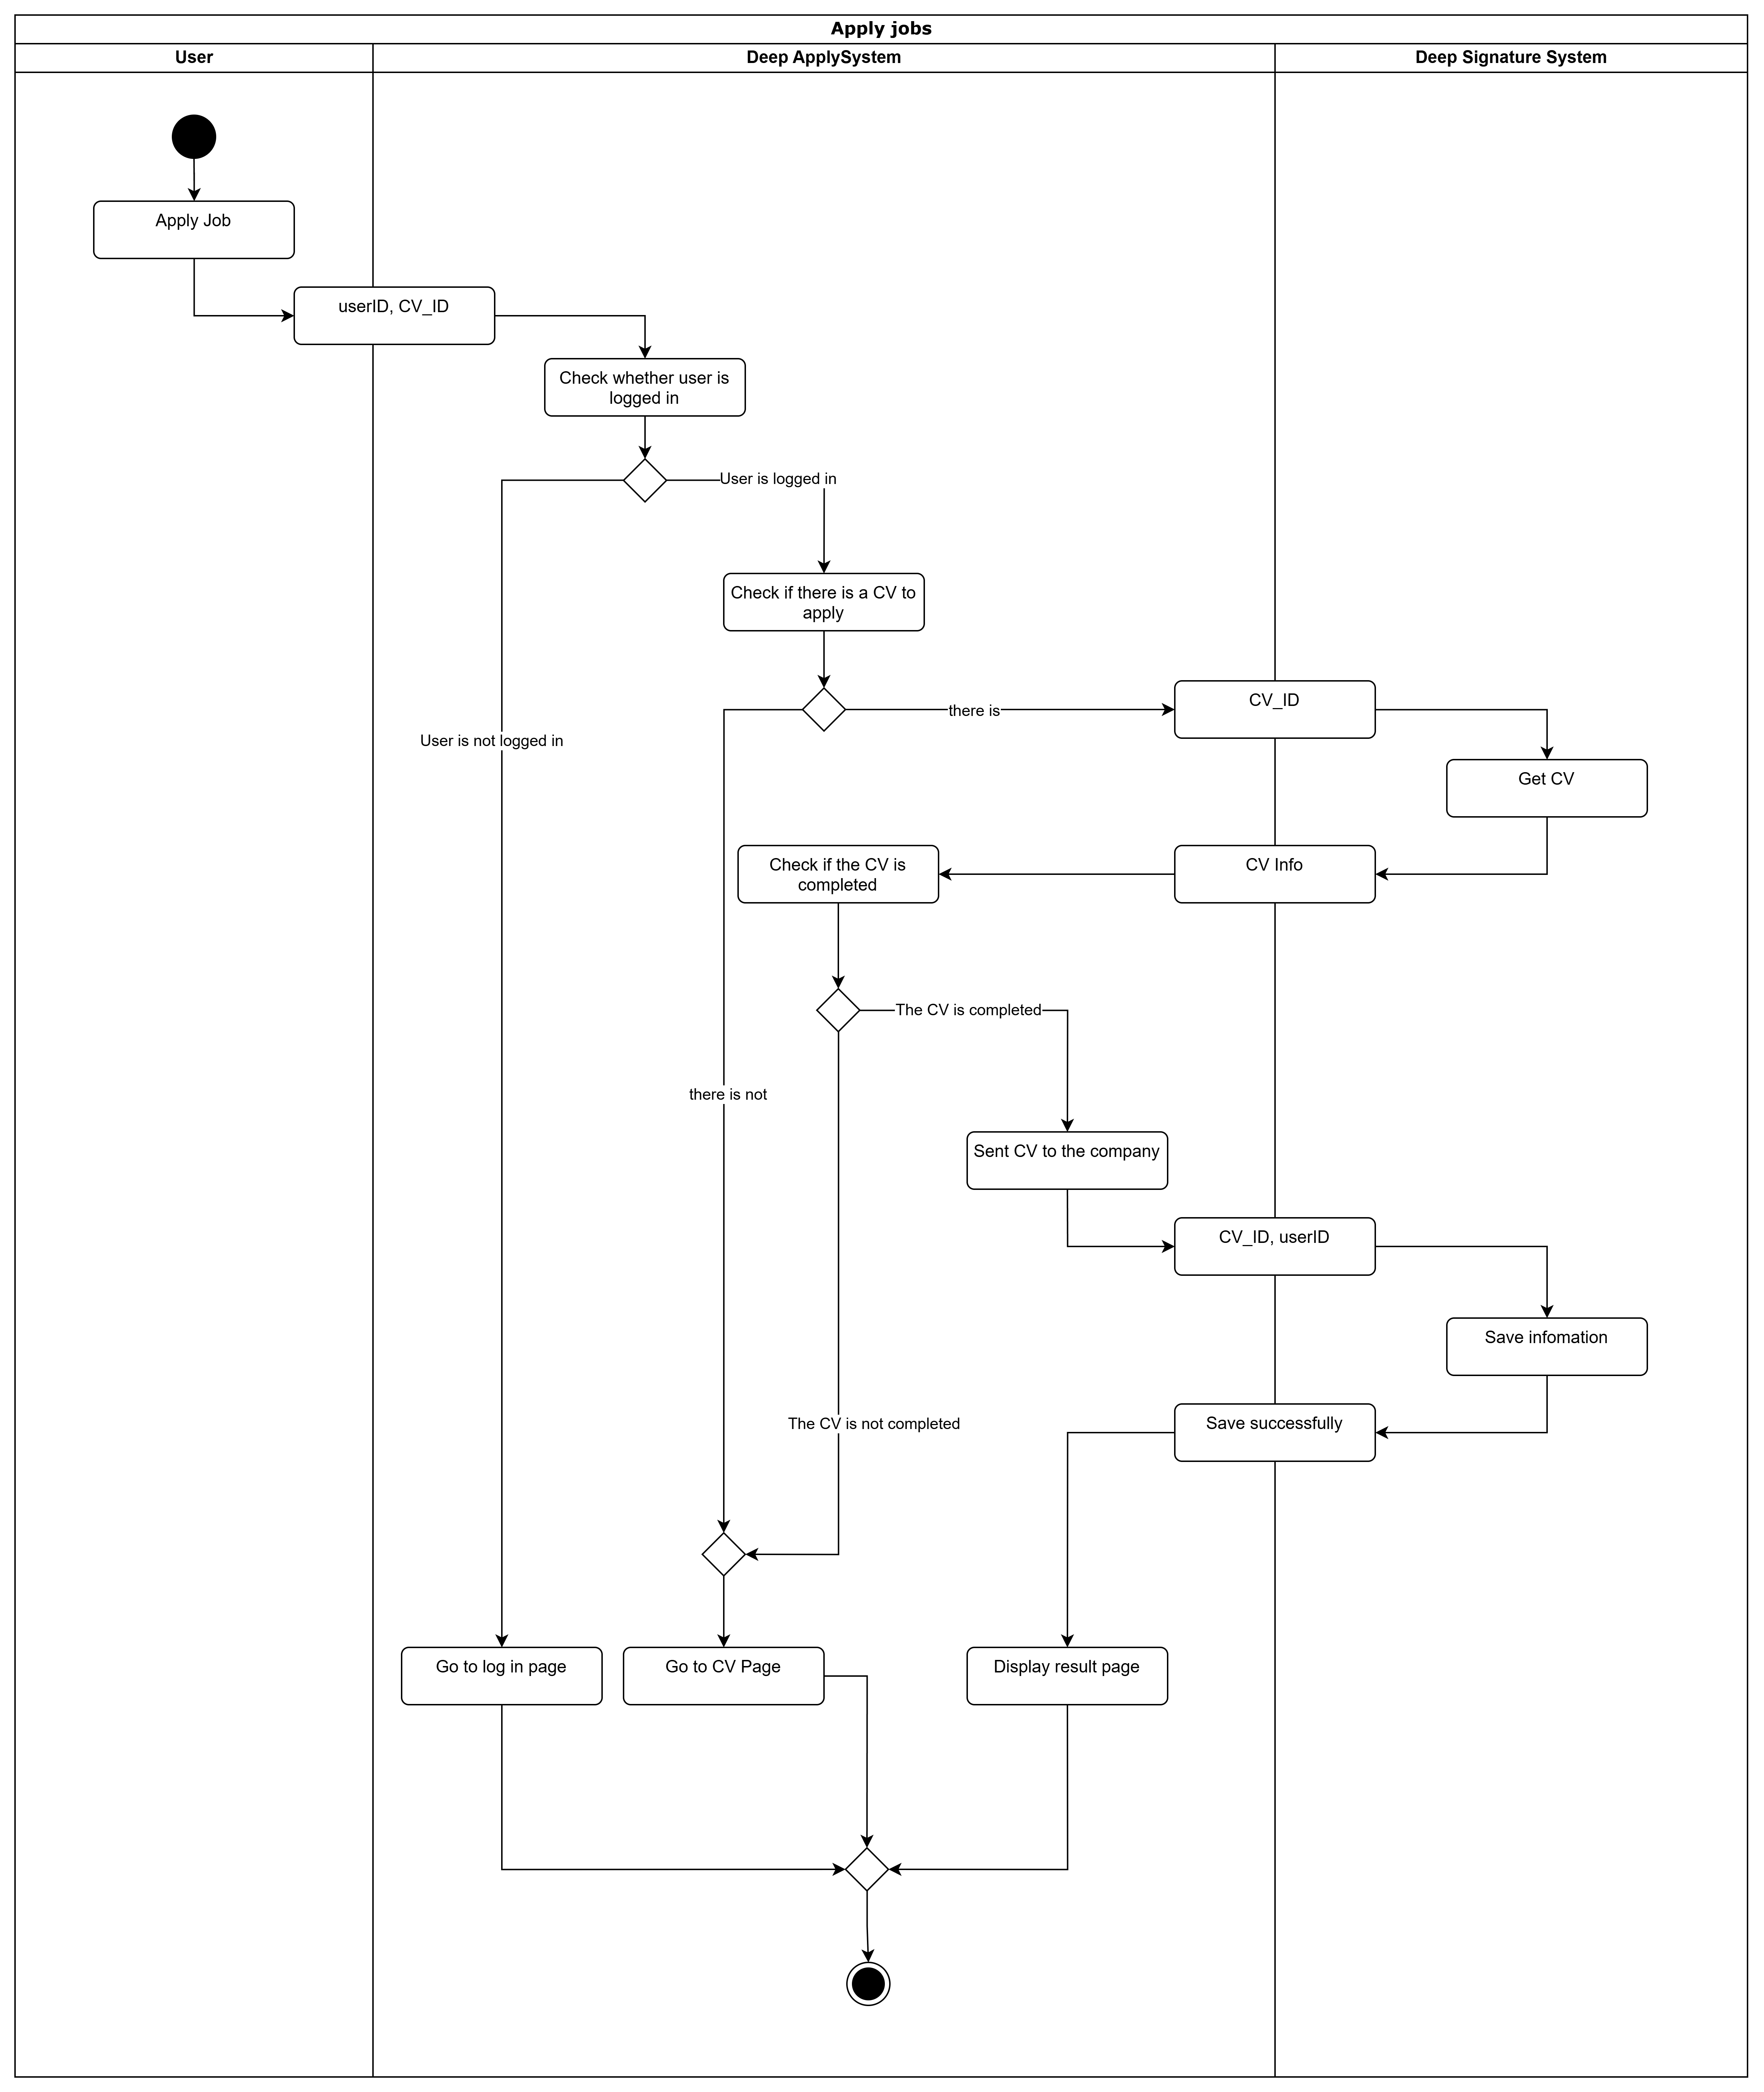
\includegraphics[scale=0.08]{img/Apply_jobs_Activity.png}
    \caption{Lược đồ hoạt động về Ứng tuyển công việc}
\end{figure}

Sau khi ứng tuyển cho một bài đăng tuyển dụng trên trang web, hệ thống sẽ kiểm tra người đã đăng nhập hay chưa. Nếu chưa người dùng được đến trang đăng nhập của trang web để thực hiện đăng nhập tài khoản. Thậm chí, nếu người dùng vẫn chưa có tài khoản trên trang web, người dùng có thể chọn phần "Đăng ký tài khoản" có trên trang Đăng nhập để thực hiện "Đăng ký tài khoản". 

Khi người dùng đăng nhập tài khoản thành công, hệ thống sẽ kiểm tra người dùng đã có CV đang trong tình trạng "Ứng tuyển" hay chưa? Trong trường hợp không có, người dùng được đưa đến trang "Quản lý CV" và cần phải tạo và hoàn thiện 1 CV mới và cho CV sang tình trạng "Ứng tuyển". Hoặc người dùng cũng có thể upload một bản CV sẵn có của bản thân lên trang web và cho nó vô tình trạng "Ứng tuyển". Sau khi tạo CV mới hay upload một CV mới lên trang web thành công, hệ thống sẽ lưu thông tin của CV vào cơ sở dữ liệu của hệ thống. 

Sau khi bấm vào nút "Ứng tuyển" trên bài đăng tuyển dụng và đã có bản CV đang trong tình trạng "Ứng tuyển", hệ thống sẽ tự động gửi thông tin và CV ứng tuyển của người dùng cho doanh nghiệp và lưu chúng vào một danh sách ứng tuyển của doanh nghiệp. Sau đó, hệ thống sẽ thông báo cho người dùng "Ứng tuyển thành công" và chuyển hướng đến trang chủ của trang web.

\subsection{Đăng bài tuyển dụng/tin tức}


\begin{figure}[H]

	\centering
    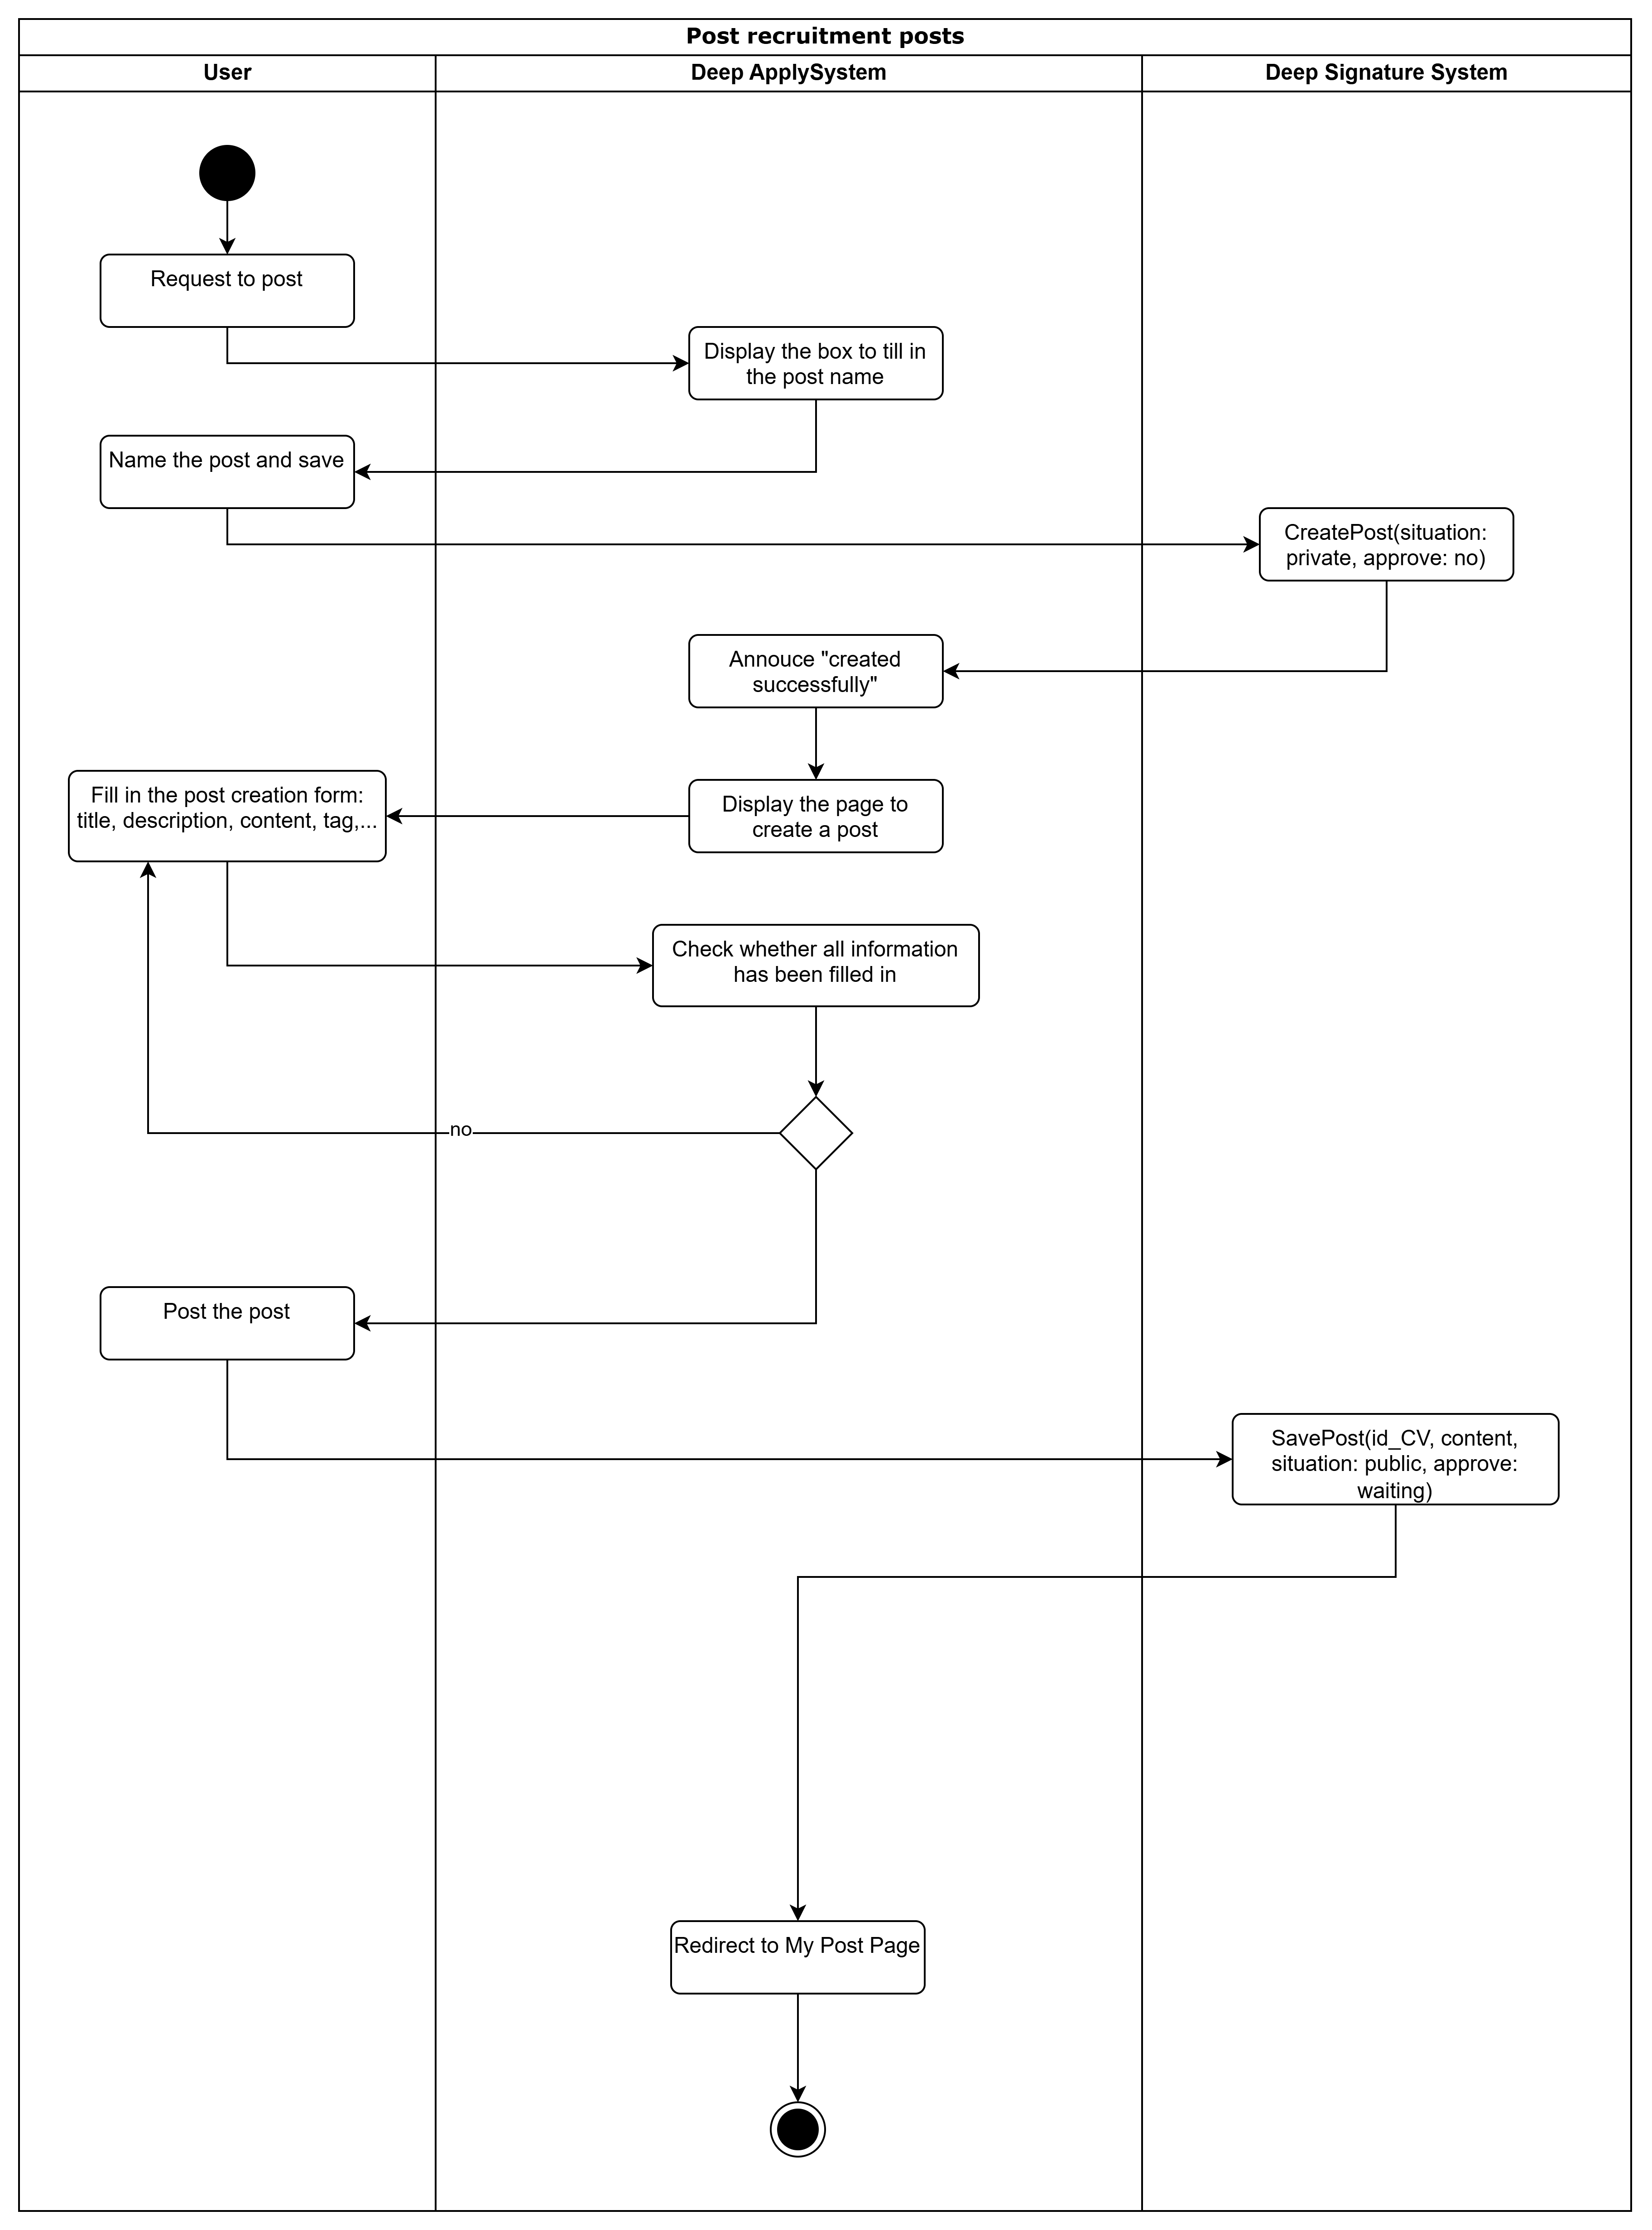
\includegraphics[scale=0.07]{img/Post_workflow.png}
    \caption{Lược đồ hoạt động về Đăng bài tuyển dụng/tin tức}
\end{figure}

Quy trình làm việc cho biểu đồ hoạt động của đăng bài tuyển dụng: Khi được yêu cầu đăng bài tuyển dụng, hệ thống sẽ hiển thị cho người dùng một trang web để đăng các bài tuyển dụng. Khi này, hệ thống sẽ cho rằng bản đang hiển thị trên trang web là bản nháp và không lưu lại vào cơ sở dữ liệu của hệ thống. Khi người dùng đặt tên cho bài đăng, hệ thống sẽ tạo và lưu dữ liệu của bài đăng vào cơ sở dữ liệu của người dùng.Ở đây, người dùng cần điền những thông tin cho bài đăng bao gồm: tiêu đề, mô tả, nội dung, yêu cầu, hình ảnh,.... 

Khi người dùng bấm vào nút đăng ở phía trên của form, hệ thống sẽ kiểm tra liệu người dùng đã điền hoàn tất chưa. Nếu người dùng chưa hoàn tất thông tin cần có, hệ thống sẽ thông báo cho người dùng "Đăng bài thất bại. Xin hãy hoàn thiện nội dung của bài đăng tuyển dụng". Nếu đã hoàn thiện nội dung của bài đăng, hệ thống sẽ thông báo cho người dùng "Đăng bài thành công. Xin vui lòng chờ admin duyệt”. Bài đăng sẽ được chuyển đến admin và chờ admin duyệt để có thể bài đăng tuyển dụng có thể thật sự xuất hiện trên trang web.



\subsection{Gửi tin nhắn}

\begin{figure}[H]

	\centering
    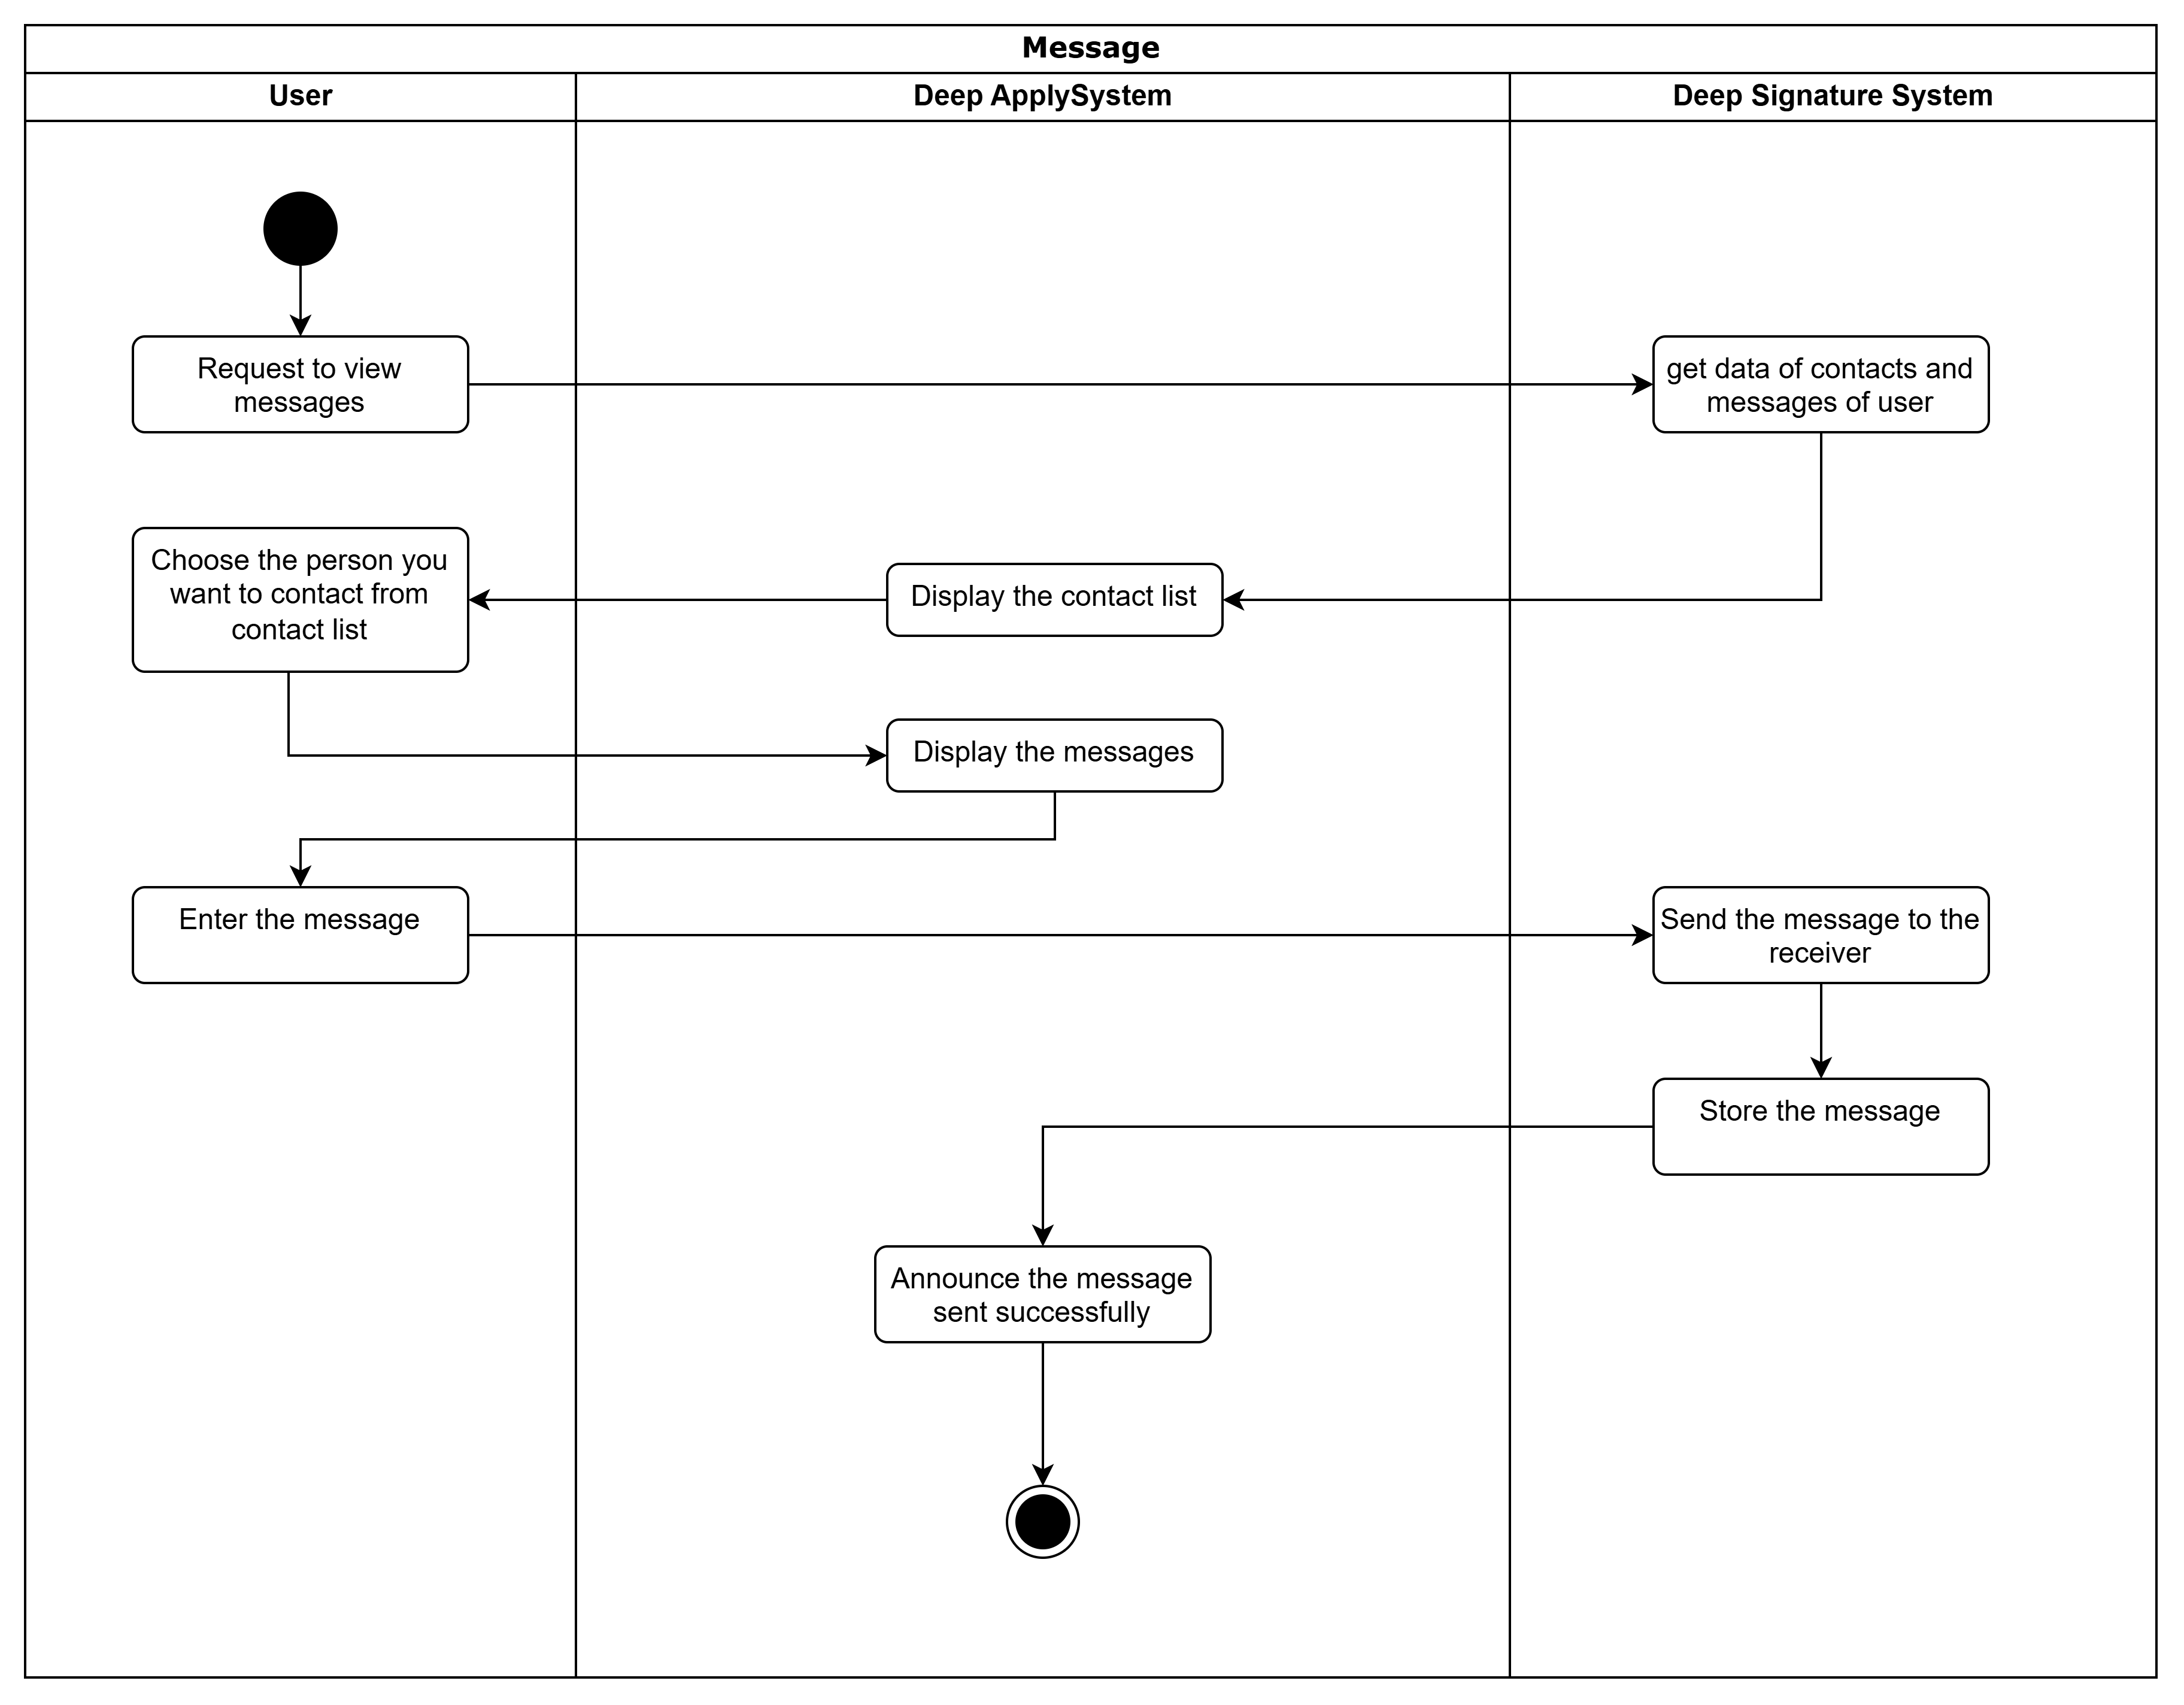
\includegraphics[scale=0.1]{img/Message_workflow.png}
    \caption{Lược đồ hoạt động về Gửi tin nhắn}
\end{figure}

Khi người dùng vào mục nhắn tin, hệ thống sẽ lấy toàn bộ tin nhắn của người dùng với những người khác và hiển thị cho người dùng danh sách những người mà họ đã giao tiếp. Người dùng sẽ chọn một người trong danh sách liên lạc. Hệ thống sẽ hiển thị cho người dùng toàn bộ tin nhắn giữa hai người. Khi người dùng gửi tin nhắn, hệ thống sẽ gửi tin nhắn đến người nhận và lưu giữ tin nhắn vào cơ sở dữ liệu của hệ thống và thông báo cho người dùng “Đã gửi thành công”.


\section{Kiến trúc hệ thống (System architecture)}

\subsection{Giới thiệu về kiến trúc hệ thống}

System Architecture (Kiến trúc hệ thống) là bản thiết kế tổng thể thể hiện cách một hệ thống phần mềm hoặc phần cứng được tổ chức, cấu trúc, và tương tác. Nó là một phần quan trọng trong phát triển và triển khai các giải pháp công nghệ, giúp đảm bảo rằng hệ thống đáp ứng các yêu cầu chức năng và phi chức năng. System Architecture đóng vai trò nền tảng trong việc xây dựng một hệ thống hiệu quả và bền vững. Kiến trúc hệ thống bao gồm 3 thành phần chính: giao diện người dùng (User Interface), máy chủ (Server), cơ sở dữ liệu (database).

Tuỳ thuộc vào mục đích và quy mô, kiến trúc hệ thống được chia làm 2 loại chính:

\begin{itemize}
    \item \textbf{Kiến trúc nguyên khối (Monolithic Architecture):} mọi thành phần của ứng dụng được xây dựng trong cùng một khối duy nhất, thích hợp cho các hệ thống nhỏ.
    \item \textbf{Kiến trúc phân tán (Distributed Architecture):} hệ thống được triển khai trên nhiều đơn vị, làm việc cùng nhau để thực hiện chức năng của hệ thống. Kiến trúc phân tán giúp tối ưu hoá hiệu năng, giảm độ trễ và tăng khả năng chịu lỗi của hệ thống, đồng thời cho phép hệ thống dễ dàng mở rộng khi quy mô người dùng và dữ liệu gia tăng.
\end{itemize}

Một kiến trúc hệ thống tốt sẽ giúp tối ưu hiệu năng, giảm độ trễ và tăng khả năng, tốc độ xử lý của hệ thống, cho phép hệ thống mở rộng dễ dàng khi quy mô người dùng và dữ liệu gia tăng. Việc cấu trúc rõ ràng giúp cho các kỹ sư dễ dàng sửa lỗi và cập nhật hệ thống. Kiến trúc đóng vai trò trong việc bảo vệ dữ liệu và ngăn chặn các mối đe doạ bên ngoài.

\subsection{Kiến trúc phân lớp (Layered architecture)}

Kiến trúc phân lớp là một kiến trúc phổ biến từ những năm 90 cho đến nay. Mỗi lớp trong kiến trúc này có chức năng riêng và tương tác với lớp ngay trên hoặc dưới nó. Các thành phần (component) trong kiến trúc phần lớp được tổ chức thành các lớp logic ngang, mỗi lớp sẽ thực hiện một vai trò cụ thể trong ứng dụng.

Kiến trúc phân lớp thường có 4 lớp tiêu chuẩn gồm: Presentation Layer, Business Layer, Persistence Layer và Database Layer. Dưới đây là một kiến trúc phân lớp tiêu chuẩn:

\begin{figure}[H]

	\centering
    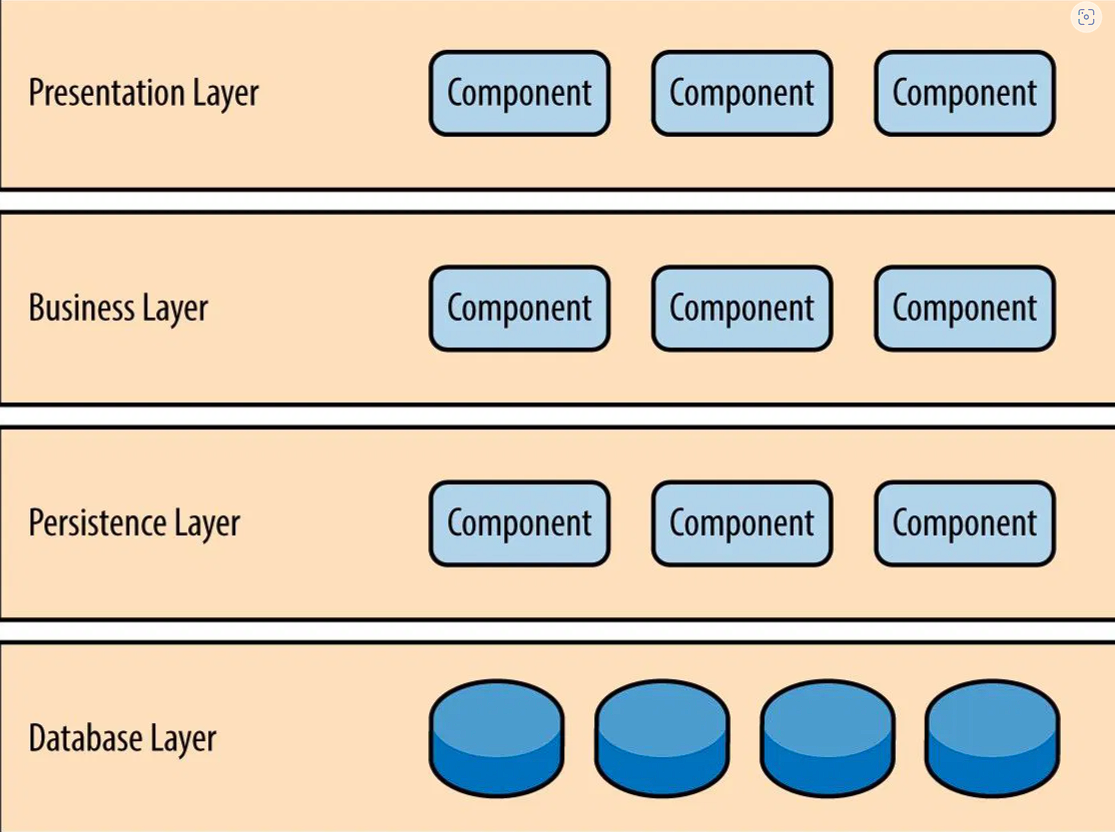
\includegraphics[scale = 0.3]{img/Layered_Architecture.png}
    \caption{Mô hình một kiến trúc phân lớp tiêu chuẩn}

\end{figure}

\begin{enumerate}
    \item \textbf{Presentation Layer:} gồm các thành phần như giao diện người dùng (UI), trình duyệt web, ứng dụng điện thoại,.... Lớp này có chức năng hiển thị thông tin và kết quả từ lớp logic của người dùng và chuyển dữ liệu của người dùng nhập vào lớp logic.
    \item \textbf{Business Layer:} Có nhiệm vụ xử lý các logic nghiệp vụ, nhận yêu cầu từ Presentation Layer, xử lý nó và gửi yêu cầu tương ứng đến Persistence Layer.
    \item \textbf{Persistence Layer:} Đảm nhiệm việc gửi các yêu cầu đến Database Layer để thực hiện các thao tác liên quan đến dữ liệu.
    \item \textbf{Database Layer:} Bao gồm cơ sở dữ liệu và các thành phần liên quan như hệ cơ sở dữ liệu. Có nhiệm vụ quản lý cơ sở dữ liệu, thực hiện thao tác đọc và ghi dữ liệu, triển khai các truy vấn và lưu trữ dữ liệu theo cách được định nghĩa từ Persistence Layer.
\end{enumerate}


\subsection{Kiến trúc hướng sự kiện (Event-driven Architecture)}

Kiến trúc hướng sự kiện là một mô hình thiết kế phần mềm tập trung vào việc tạo ra, phát hiện và phản ứng với các sự kiện. Kiến trúc hướng sự kiện bao gồm các thành phần hay dịch vụ của hệ thống giao tiếp với nhau chủ yếu thông qua việc sản xuất và tiêu thụ các sự kiện. Thay vì gọi trực tiếp đến các dịch vụ hoặc module khác, các thành phần trong hệ thống sẽ giao tiếp với nhau thông qua việc phát ra và lắng nghe các sự kiện. Các "sự kiện" này có thể là các hành động của người dùng, việc cập nhật dữ liệu hoặc các thông báo từ hệ thống khác.

Kiến trúc hướng sự kiện được phân loại dựa trên cấu trúc liên kết giữa các thành phần (component) trong hệ thống với nhau bao gồm 2 mô hình phổ biến là: Broker Topology và Mediator Topology.

\subsubsection{Quy trình làm việc của Broker Topology}

\begin{figure}[htp!]

	\centering
    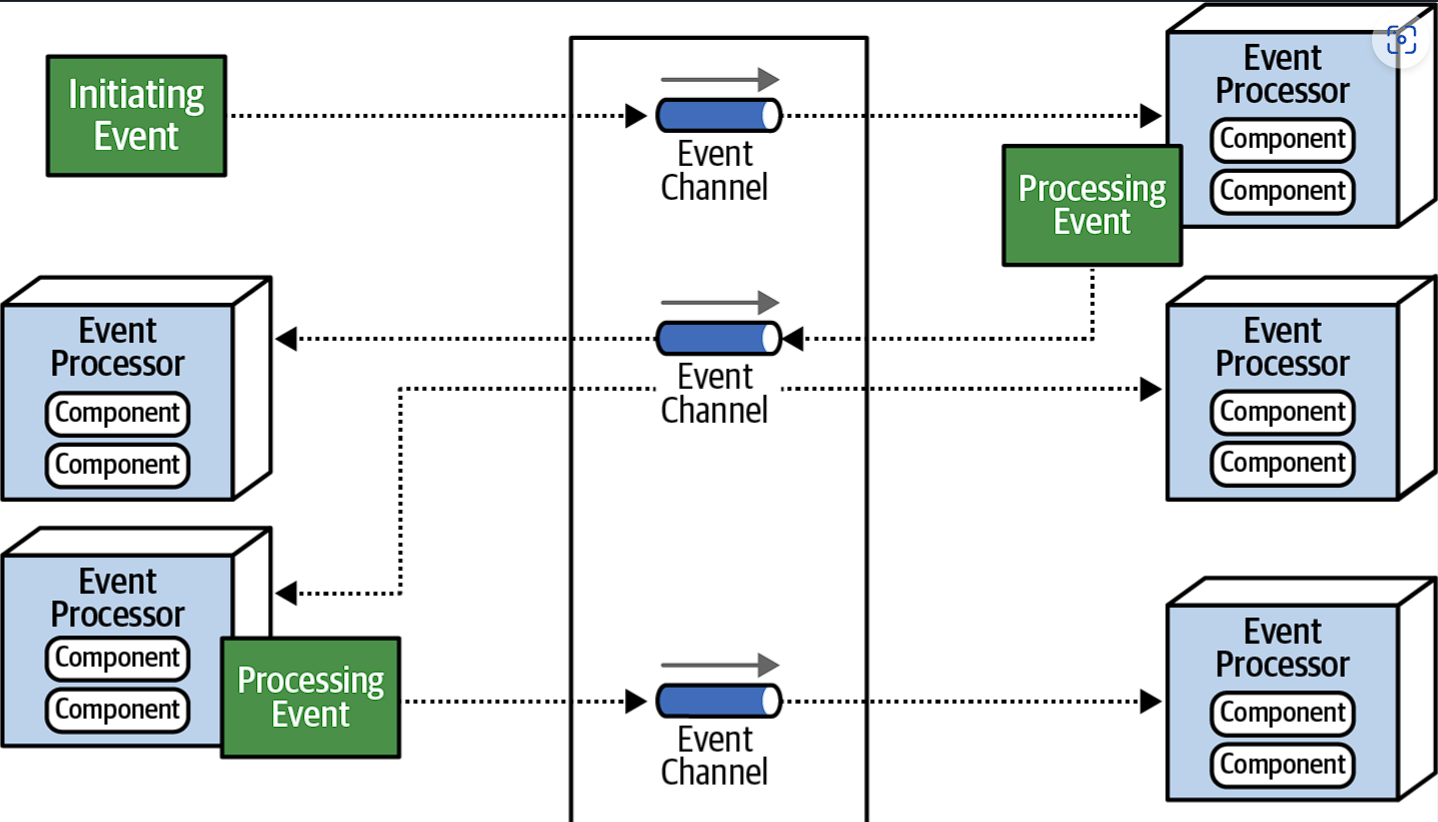
\includegraphics[scale=0.3]{img/Broker_Topology.png}
    \caption{Quy trình làm việc của Broker Topology}
\end{figure}


\subsubsection{Quy trình làm việc của Mediator Topology}

\begin{figure}[htp!]

	\centering
    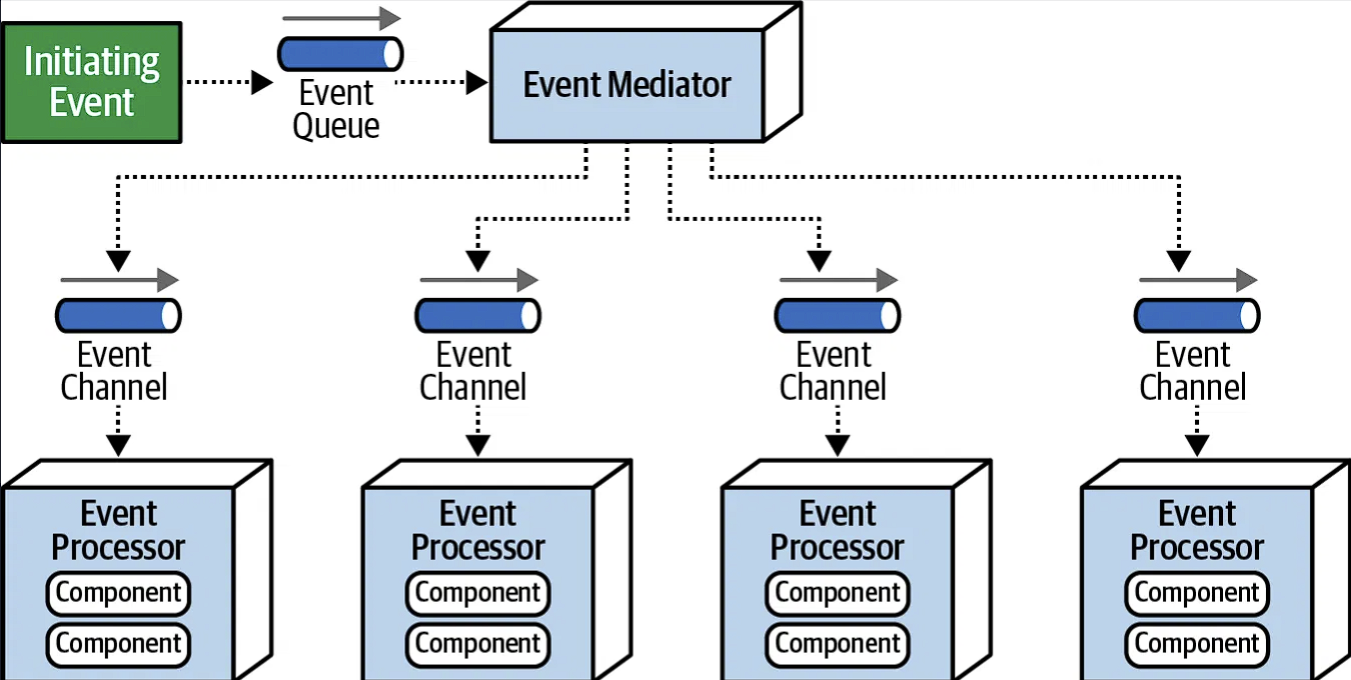
\includegraphics[scale=0.3]{img/Mediator_Topology.png}
    \caption{Quy trình làm việc của Mediator Topology}
\end{figure}


\subsection{Kiến trúc vi nhân (Microkernel Architecture)}


Kiến trúc vi nhân là một mô hình kiến trúc phần mềm, trong đó, hệ thống được phân chia thành các module hoặc các thành phần nhỏ và độc lập (được gọi là microkernel). Nó chịu trách nhiệm cho các nhiệm vụ riêng biệt như xử lý dữ liệu, lưu trữ dữ liệu,.... Kiến trúc vi nhân rất linh hoạt và dễ mở rộng, nó cho phép nhà phát triển hoặc người dùng dễ dàng thêm các chức năng và tính năng bổ sung vào ứng dụng hiện có dưới dạng tiện ích (extensions) hoặc plug-in mà không ảnh hưởng đến chức năng cốt lõi của hệ thống.


\begin{figure}[H]

	\centering
    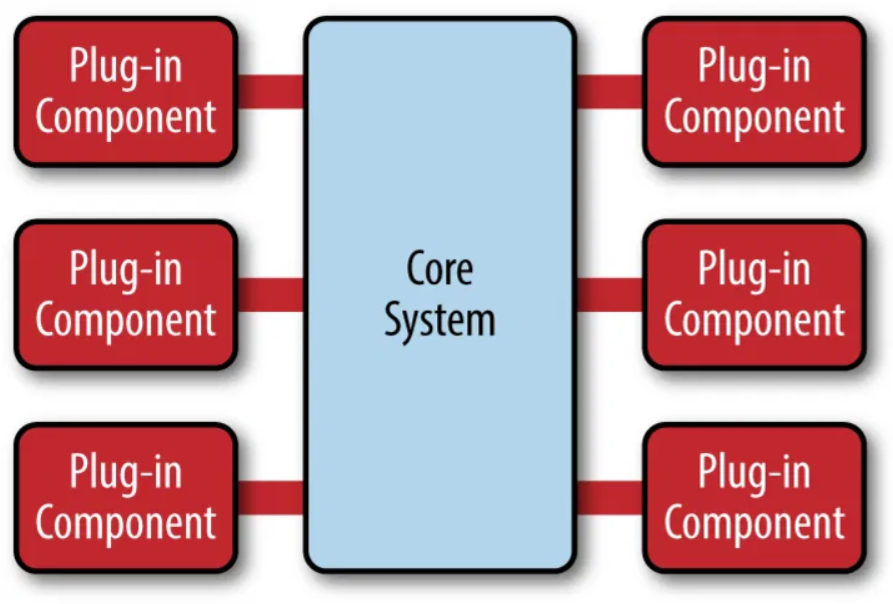
\includegraphics[scale=0.4]{img/microkernel_architecture.png}
    \caption{Cấu trúc về kiến trúc vi nhân}
\end{figure}
\newpage

Kiến trúc vi nhân bao gồm 4 thành phần chính:
\begin{itemize}
    \item \textbf{Core system (Hệ thống lõi):} bao gồm các chức năng tối thiểu cần thiết để giúp hệ thống có thể hoạt động được.
    \item \textbf{Plug-in:} bao gồm các thành phần độc lập, có khả năng xử lý chuyên biệt, có các tính năng bổ sung và mã tùy chỉnh nhằm nâng cao hoặc mở rộng hệ thống cốt lõi. Bên cạnh đó, các plug-in phải độc lập với nhau và không phụ thuộc lẫn nhau trong quá trình hoạt động.
    \item \textbf{Register:} core system sẽ dùng registry để xác định plug-in nào đang khả dụng và kết nối tới plug-in đó như thế nào.
    \item \textbf{Contract:} thể hiện mối quan hệ giữa hệ thống lõi và các mô-đun plug-in bao gồm hành vi, giao thức truy cập từ xa từ hệ thống lõi tới plug-in, dữ liệu đầu vào và đầu ra của các plug-in.
\end{itemize}

\subsection{Kiến trúc Microservice}

Kiến trúc Microservice là một phong cách kiến trúc phần mềm trong đó một ứng dụng được chia thành các dịch vụ nhỏ, độc lập, mỗi dịch vụ thực hiện một chức năng cụ thể và giao tiếp với nhau thông qua các giao diện lập trình ứng dụng (API). Các dịch vụ này có thể được phát triển, triển khai và mở rộng một cách độc lập, giúp tăng tính linh hoạt và khả năng mở rộng của hệ thống.


\begin{figure}[H]

	\centering
    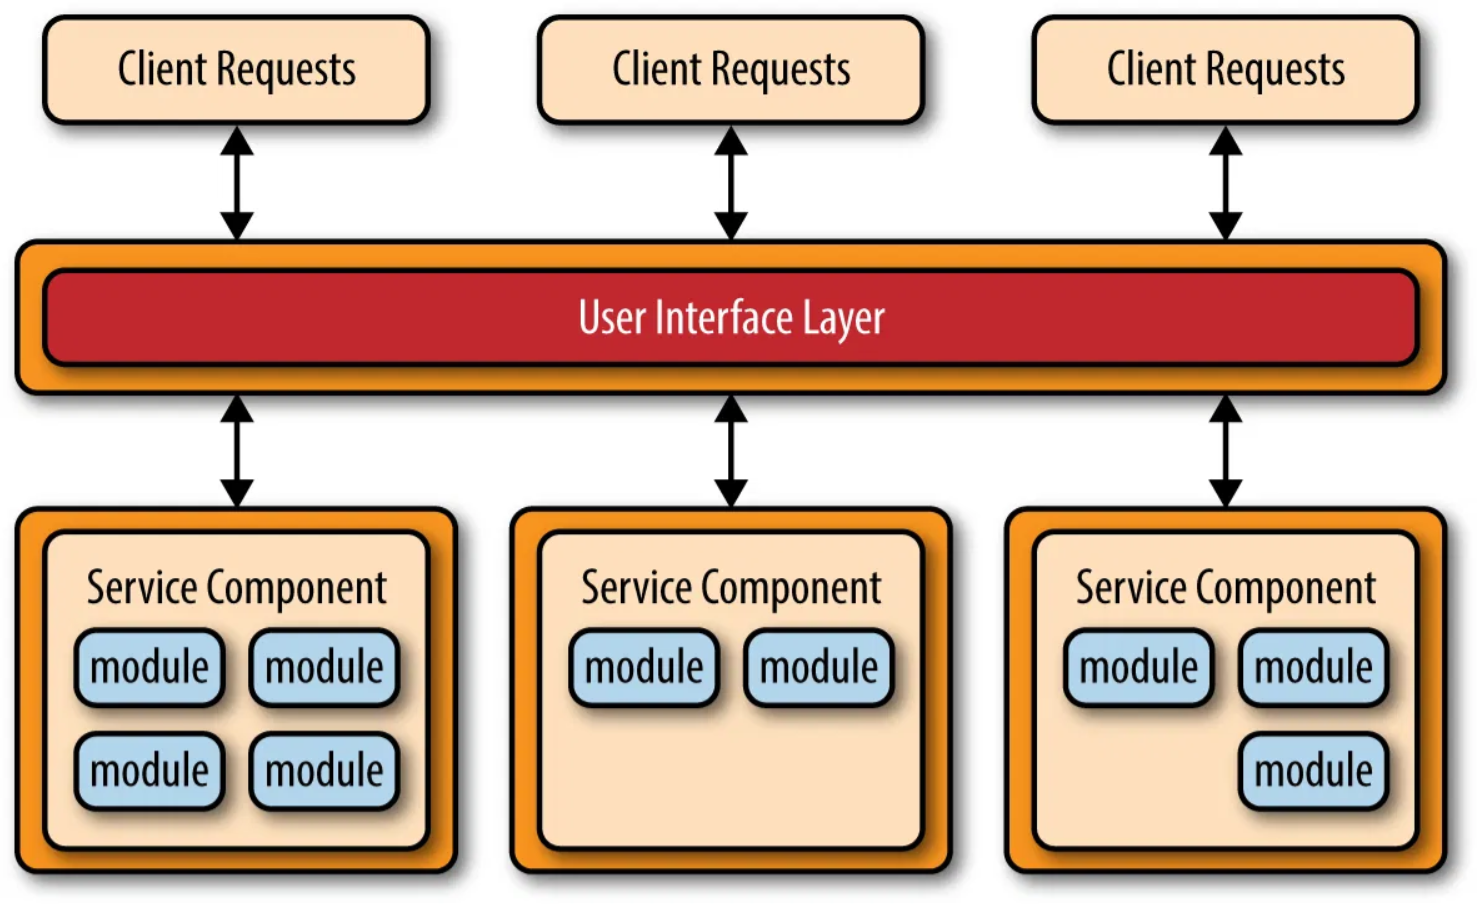
\includegraphics[scale = 0.25]{img/Microservice_Architecture.png}
    \caption{Cấu trúc về kiến trúc Microservice}
\end{figure}

Kiến trúc Microservice được xây dựng dựa trên "bounded context": Mỗi service mô hình hoá một domain hoặc một workflow. Tức là mỗi service có thể chứa mọi thứ cần thiết để hoạt động trong ứng dụng, bao gồm các class, các thành phần con trong nó và database.

Mặc dù kiến trúc Microservice rất phổ biến và mạnh mẽ nhưng đây cũng là một kiến trúc rất khó triển khai nhất. 

\subsection{Mô hình MVCs (Model - View - Controller)}

Mô hình MVCs là một mẫu kiến trúc, mô hình lập trình phổ biến được sử dụng để tạo cấu trúc cho nhiều trang web, ứng dụng tiên tiến.

MVCs được chia làm 3 phần phụ thuộc và kết nối với nhau:
\begin{itemize}
    \item \textbf{Model:} có vai trò quản lý dữ liệu và logic nghiệp vụ của ứng dụng. Nó giúp xử lý dữ liệu, tương tác với cơ sở dữ liệu và thực hiện các thao tác nghiệp vụ.
    \item \textbf{View:} là thành phần hiển thị dữ liệu và giao diện người dùng, giúp người xem có thể xem được thông tin trang web và ứng dụng một cách trực quan. Nó nhận ữ liệu từ Model và hiển thị cho người dùng, nhận các tương tác từ người dùng và chuyển tiếp đến Controller.
    \item \textbf{Controller:} có chức năng nhận các yêu cầu từ View, gọi các phương thức từ Model để xử lý dữ liệu và cập nhật View. Nó vai trò điều khiển luồng dữ liệu giữa Model và View.
\end{itemize}

\begin{figure}[H]

	\centering
    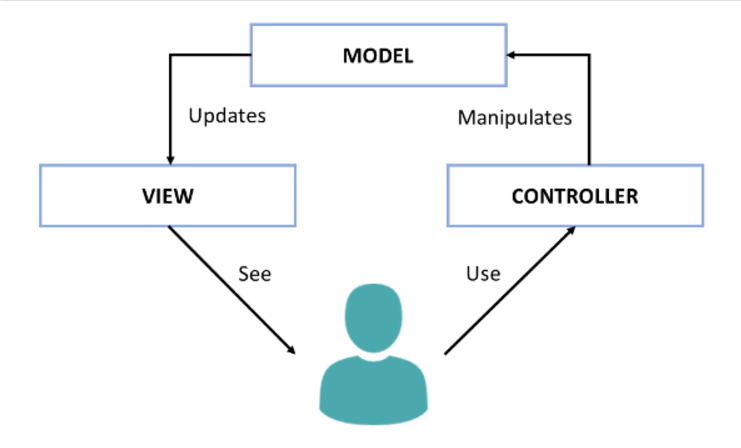
\includegraphics[scale=0.4]{img/MVCs_workflow.png}
    \caption{Quy trình làm việc của mô hình MVCs}
\end{figure}

Khi bạn gửi những yêu cầu, request đến Controller và Controller nhận được yêu cầu từ người dùng, chúng sẽ kiểm tra yêu cầu có cần lấy dữ liệu từ Model hay không. Nếu cần Controller sẽ dùng các class/function sẵn có để trả kết quả. Sau khi xử lý các dữ liệu đó, nó sẽ trả qua View để hiển thị.

Còn View sẽ chịu trách nhiệm cho phần hiển thị như thống tin dữ liệu, hình ảnh,.... Rồi trả về GUI Content để Controller đưa kết quả lên Browser. Trình duyệt sẽ tiếp nhận dữ liệu và trả lại kết quả tìm kiếm cho người dùng.

\subsection{Thiết kế kiến trúc hệ thống}

Ở đồ án này tôi sử dụng mô hình kiến trúc MVCs vì những lợi ích trong việc phát triển phần mềm, đặc biệt trong các ứng dụng giao diện người dùng. Nó cho phép các lập trình viên phân tách rõ ràng cấu trúc model, data, giao diện người dùng và nghiệp vụ. MVCs cũng cung cấp đa dạng hình thức View cho nhiều đối tượng khác nhau. Thậm chí, ta có thể tái sử dụng các Model hay View mà không bị ảnh hưởng tới các thành phần khác. Do bởi Controller và Model độc lập với View, nên nó giúp cho hệ thống dễ dàng mở rộng và kiểm thử hơn.

\subsubsection{Dưới đây là sự so sánh MVCs với các kiến trúc khác:}


\begin{table}[H]
    \centering
    \begin{tabular}{|>{\centering\arraybackslash}p{0.1\linewidth}|>{\centering\arraybackslash}p{0.15\linewidth}|>{\centering\arraybackslash}p{0.15\linewidth}|>{\centering\arraybackslash}p{0.15\linewidth}|>{\centering\arraybackslash}p{0.13\linewidth}|>{\centering\arraybackslash}p{0.13\linewidth}|} \hline 
         Tiêu chí&  MVCs&  Layered Architecture&   Microservices Architecture&  Microkernel Architecture& Event-driven Architecture\\ \hline 
         Mục tiêu thiết kế&  Tách rõ ràng giữa Model, View, Controller&  Tách biệt các tầng (layer) theo chức năng logic&  Tách biệt theo dịch vụ độc lập&  Tách biệt giữa kernel (cốt lõi) và các plugin& Tách biệt thành phần sản xuất \& xử lý sự kiện\\ \hline 
         Khả năng mở rộng&  Phù hợp cho ứng dụng vừa và nhỏ. Khó mở rộng khi hệ thống quá phức tạp.&  Dễ mở rộng theo chiều dọc nhưng khó mở rộng theo chiều ngang (tầng thường bị phụ thuộc lẫn nhau).&  Rất cao (dịch vụ độc lập)&  Cao (thêm plugin hoặc mở rộng kernel)& Cao (có thể thêm nhiều producer hoặc consumer)\\ \hline 
         Tính linh hoạt&  Tốt, nhưng Controller thường phụ thuộc vào logic business&  Trung bình (thay đổi 1 tầng có thể ảnh hưởng tầng khác)&  Cao, nhưng phức tạp hơn trong việc phối hợp&  Trung bình (phụ thuộc vào cốt lõi kernel)& Cao, nhưng khó quản lý các sự kiện phức tạp\\ \hline 
         Độ phức tạp khi triển khai&  Đơn giản, dễ hiểu. Thích hợp cho ứng dụng nhỏ và trung bình.&  Đơn giản trong hệ thống nhỏ, nhưng phức tạp dần khi có nhiều tầng phụ thuộc lẫn nhau.&  Phức tạp cao, yêu cầu quản lý giao tiếp giữa các service.&  Đơn giản khi thiết kế lõi, nhưng phức tạp hơn khi thêm plugin.& Phức tạp khi xử lý đồng bộ nhiều sự kiện và quản lý message broker.\\ \hline 
         Khả năng tái sử dụng&  Cao ở Model và View.&  Cao ở các tầng logic.&  Cao (để chia sẻ hoặc sử dụng lại các dịch vụ)&  Cao (plugin để tái sử dụng)& Thấp nếu không chuẩn hóa sự kiện\\ \hline 
         Dễ bảo trì&  Dễ bảo trì với các ứng dụng nhỏ, khó bảo trì khi mở rộng hệ thống phức tạp.&  Dễ bảo trì với cấu trúc phân tầng rõ ràng, nhưng phụ thuộc lẫn nhau có thể gây khó khăn.&  Dễ bảo trì nhờ tính độc lập của từng microservice, nhưng cần chú ý sự đồng nhất trong các giao diện API.&  Dễ bảo trì, plugin có thể thay thế hoặc nâng cấp mà không ảnh hưởng lõi.& Phụ thuộc vào cách tổ chức các sự kiện và logic xử lý.\\ \hline
    \end{tabular}
    \caption{So sánh MVCs với các kiến trúc khác}
    \label{tab:MVCs_comparasion}
\end{table}

Chính vì các lý do trên, nên tôi đã sử dụng kiến túc MVCs trong quá trình thiết kế kiến trúc hệ thống của trang web. Hình dưới đã minh hoạ tổng quan và khái quát cách tôi sẽ triển khai hệ thống của mình. Sẽ có 4 View cho 4 đối tượng khác nhau gồm: User/Applicant, Admin, Recruiter/Company và external stakeholder. Với những đối tượng như User/Applicant, Admin, Recruiter/Company, họ cần phải đăng nhập vào trang web để có View của mình. Còn đối với External Stakeholder, họ là đối tượng không cần đăng nhập nhưng vẫn có thể quan sát được trang web với một View riêng. Về Front-end, sẽ được thiết kế và triển khai bằng ngôn ngữ ReactJS. Front-end sẽ được kết nối với back-end - sử dụng MongoDB thông qua HTTPS. Các dữ liệu của back-end cũng sẽ được lưu giữ trong cơ sở dữ liệu của MongoDB.

\subsubsection{Thiết kế kiến trúc hệ thống}

\begin{figure}[H]

	\centering
    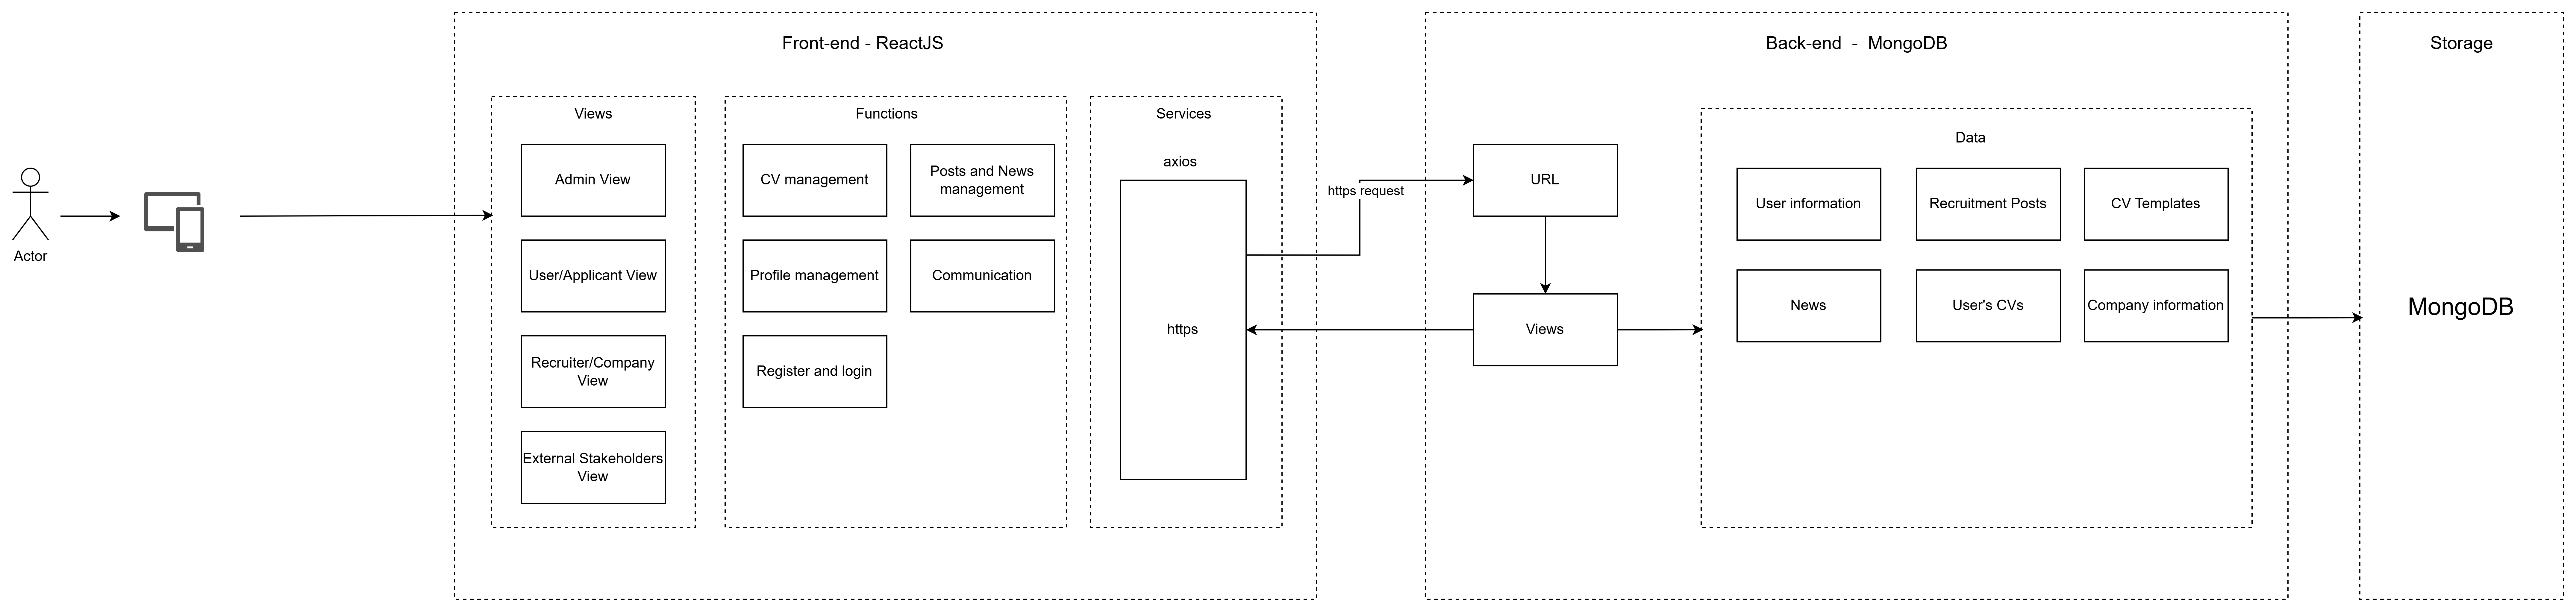
\includegraphics[angle=90,scale=0.07]{img/system_architecture.png}
    \caption{Kiến trúc hệ thống của trang web}
\end{figure}




\section{Lược đồ lớp (Class diagram)}

\subsection{Khái quát về class diagram}

Class Diagram là một loại biểu đồ trong kỹ thuật phần mềm, được sử dụng để mô tả cấu trúc và mối quan hệ giữa các lớp trong một hệ thống phần mềm. Nó là một phần quan trọng của mô hình hóa phân cấp, hay còn được gọi là UML (Unified Modeling Language), được sử dụng rộng rãi trong việc phát triển phần mềm.

Class diagram (biểu đồ lớp) đóng vai trò thiết yếu trong việc mô hình hóa cấu trúc của các hệ thống phần mềm. Nó giúp các nhà phát triển phần mềm có cái nhìn tổng quan về kiến trúc của hệ thống. Nó cung cấp thông tin chi tiết về cách các đối tượng trong hệ thống tương tác với nhau, từ đó hỗ trợ việc lập kế hoạch, thiết kế và triển khai một cách hiệu quả.




\subsection{Thiết kế lược đồ lớp}

\begin{figure}[H]

	\centering
    \includegraphics[angle = 90,scale=0.05]{img/ClassDiagram.png}
    \caption{Lược lớp của hệ thống}
\end{figure}




\subsection{Lớp điều khiển (Controller Layer)}

\begin{figure}[H]

	\centering
    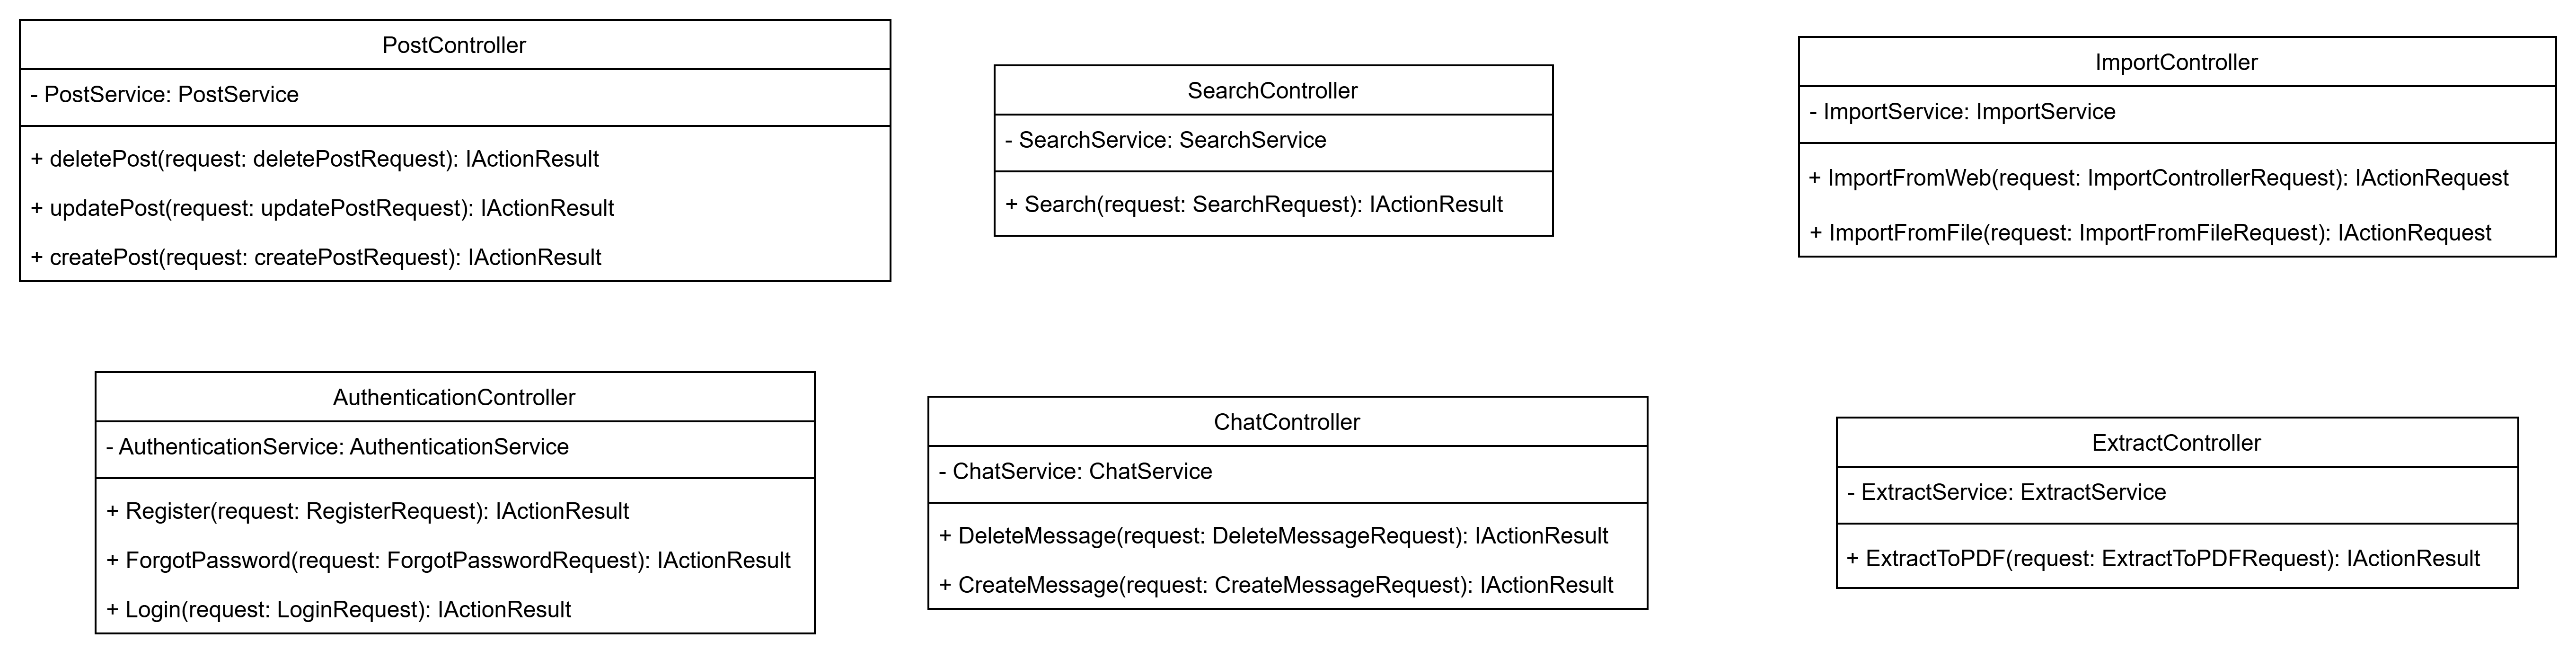
\includegraphics[scale=0.08]{img/Controller_view.png}
    \caption{Lớp điều khiển của lược đồ lớp}
\end{figure}

Lớp điều khiển (Controller Layer) là lớp chịu trách nhiệm cho việc tiếp nhận yêu cầu từ hành động cụ thể của người dùng lên giao diện của trang web và gửi lại phản hồi cho người dùng. Hệ thống sẽ tiếp nhận yêu cầu của người dùng, gọi các dịch vụ từ lớp dịch vụ, xử lý và phản hồi yêu cầu của người dùng thông qua hiển thị thông báo lên trang web.


\subsection{Lớp dịch vụ (Service Layer) }

\begin{figure}[H]

	\centering
    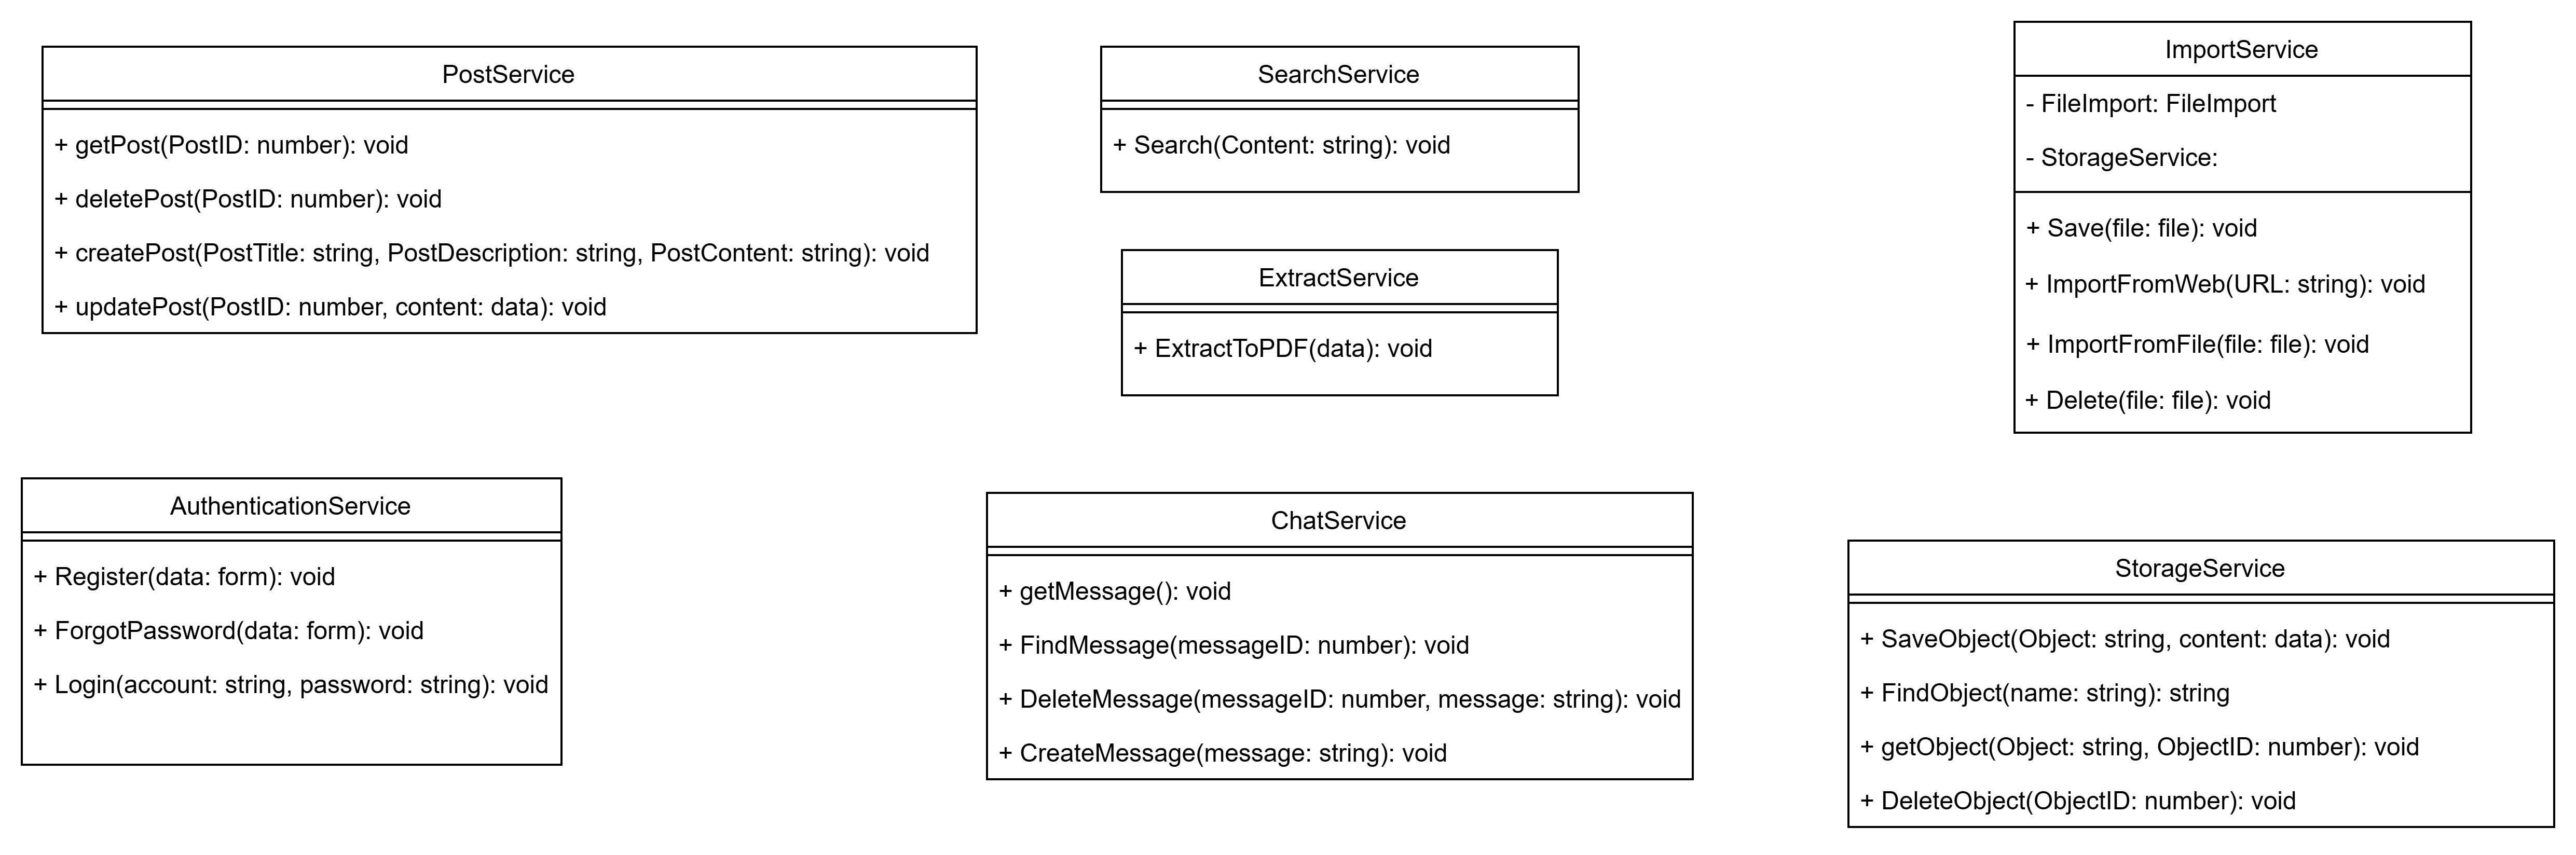
\includegraphics[scale=0.06]{img/Service_layer.png}
    \caption{Lớp dịch vụ của lược đồ lớp}
\end{figure}

Lớp dịch vụ (Service Layer) là lớp trung gian giữa controller và model. Nó chứa toàn bộ logic nghiệp vụ (business logic) của ứng dụng. Nó giúp xử lý yêu cầu từ lớp Controller và giao tiếp với lớp dữ liệu (Model Layer)  để truy xuất dữ liệu.


\subsection{Lớp dữ liệu (Model Layer)}

\begin{figure}[H]

	\centering
    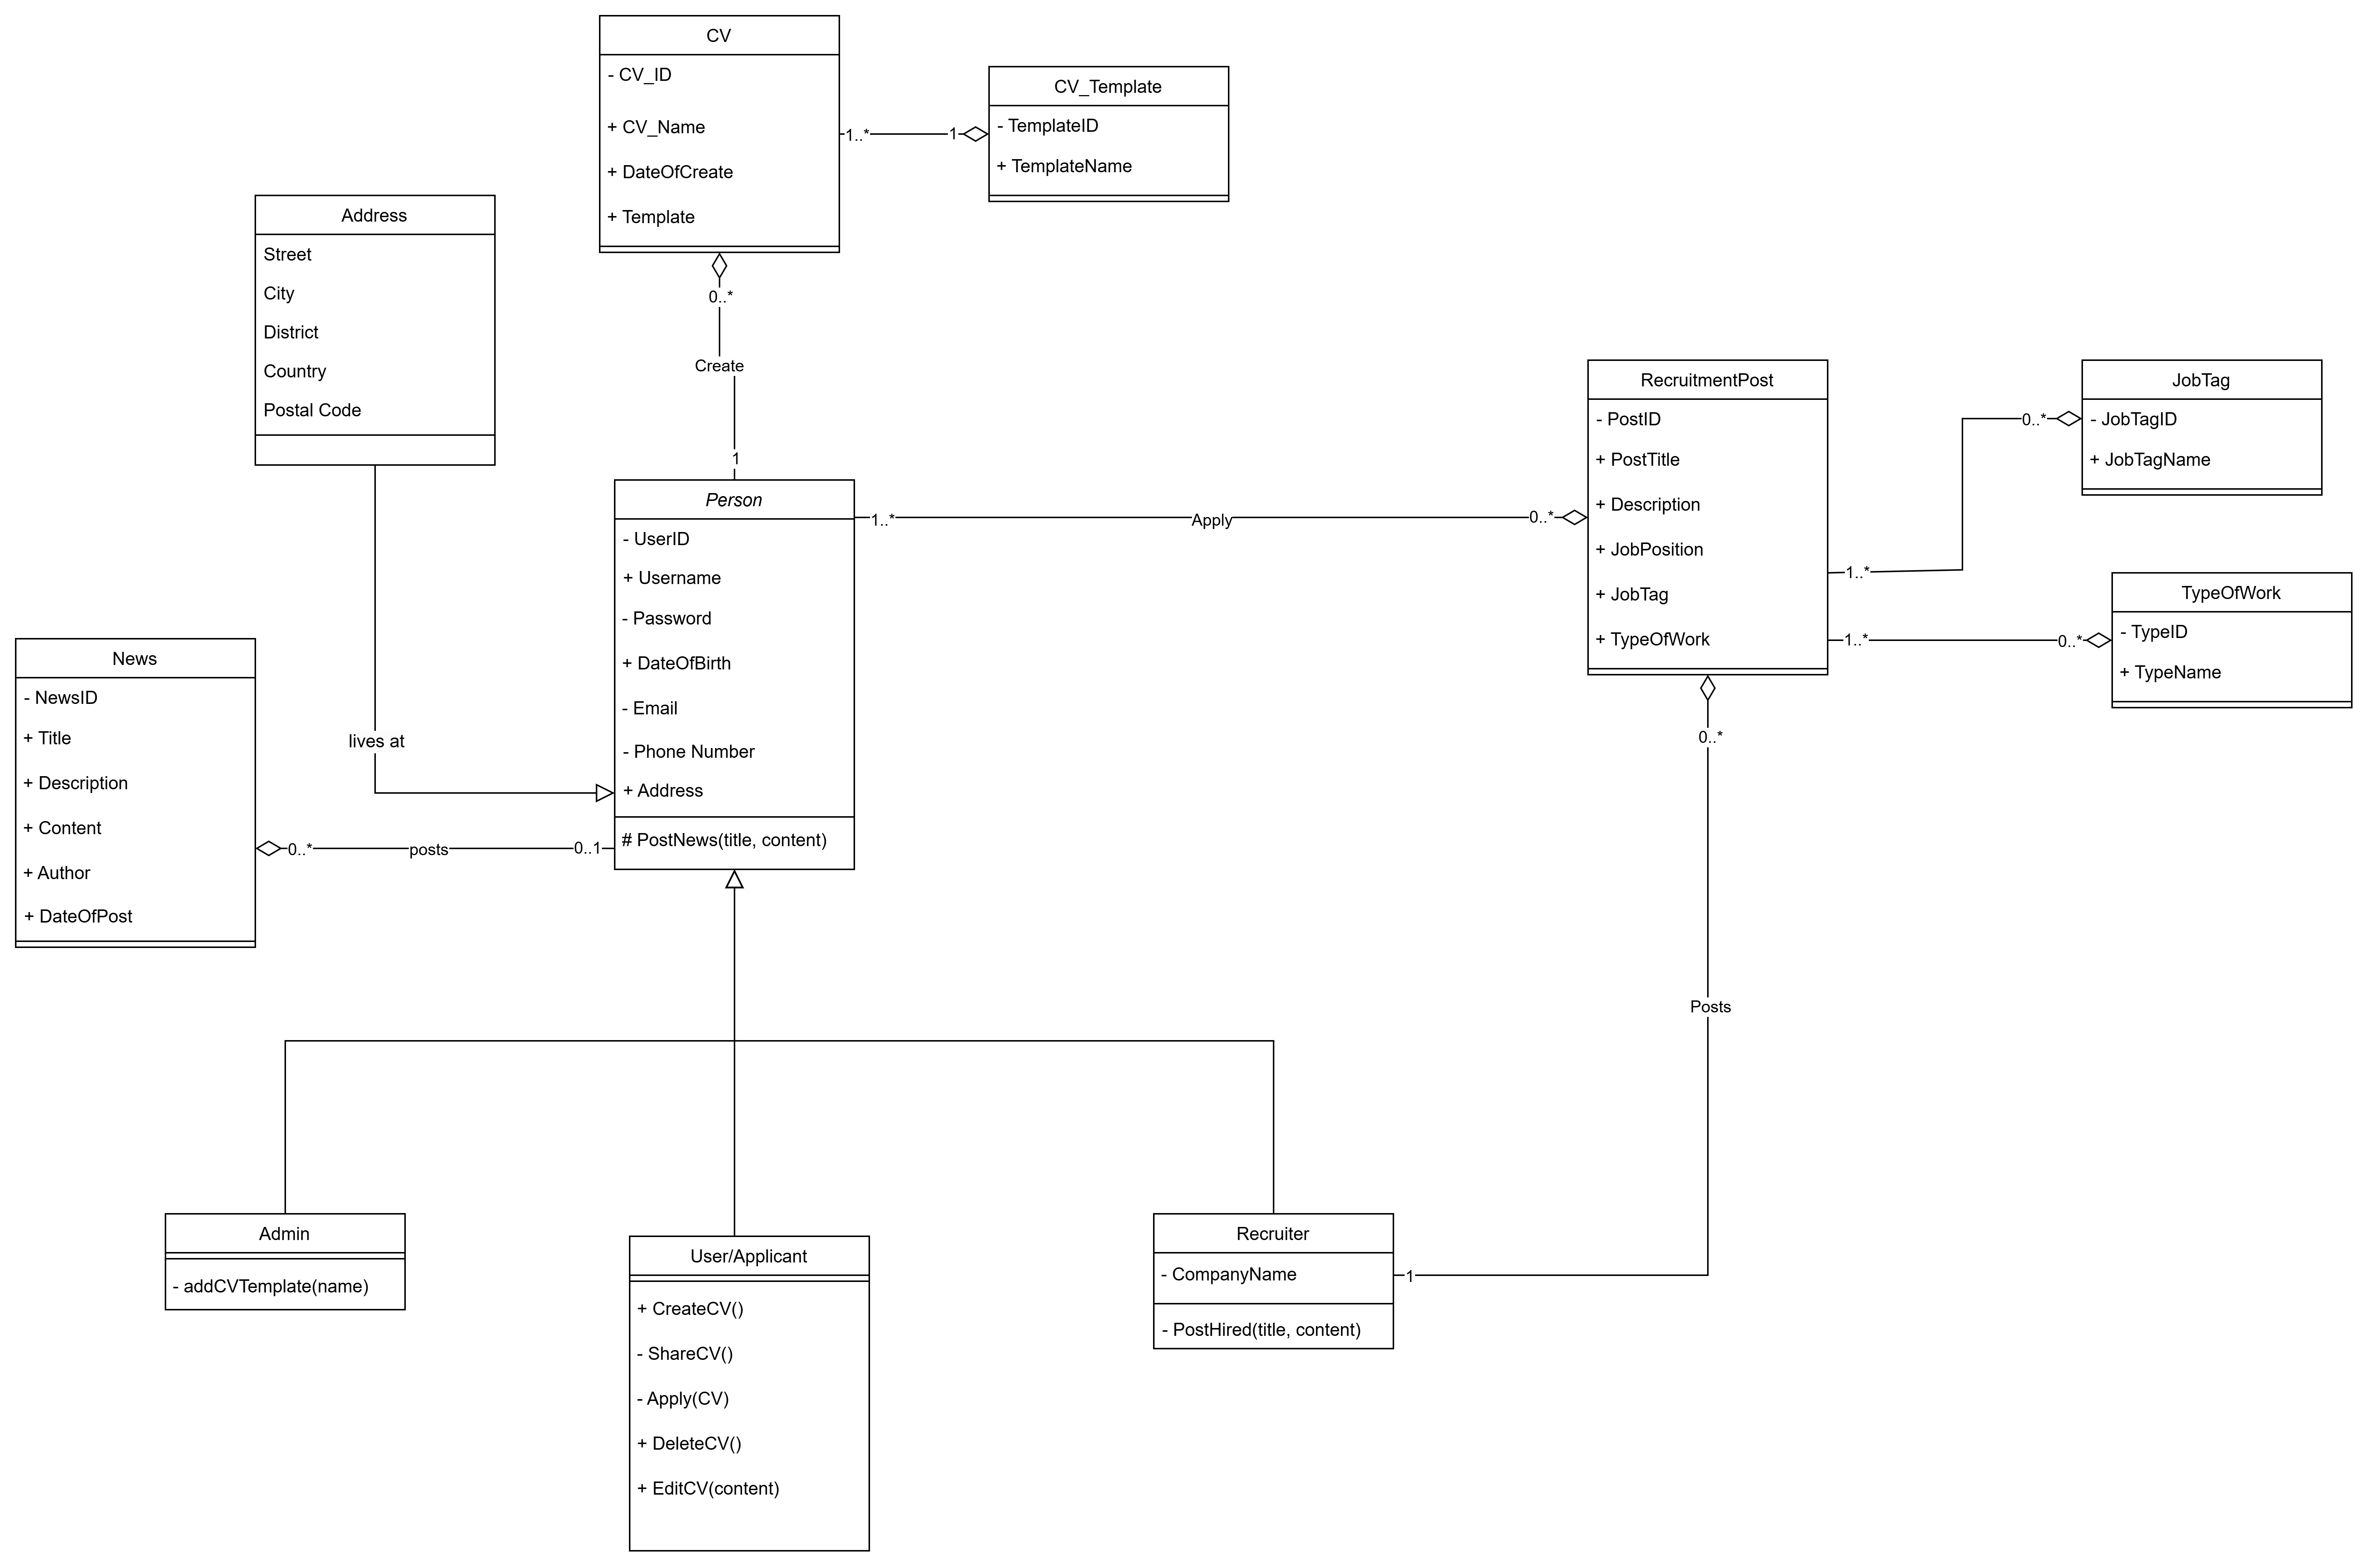
\includegraphics[scale=0.07]{img/Overview_classDiagram.png}
    \caption{Lớp dữ liệu của lược đồ lớp}

	
\end{figure}

Lớp dữ liệu (Model Layer) là lớp chứa các đối tượng mô hình hóa dữ liệu trong hệ thống. Các class trong Model Layer đại diện cho các thực thể trong cơ sở dữ liệu bao gồm các thực thể: news, user, CV, CV template, recruitementPost, JobTag, TypeOfWork. Toàn bộ dữ liệu của các thực thể trong lớp dữ liệu đều được lưu trữ trong StorageService.

\section{Lược đồ tuần tự (Sequence diagram)}


\subsection{Đăng ký tài khoản}

\begin{figure}[H]

	\centering
    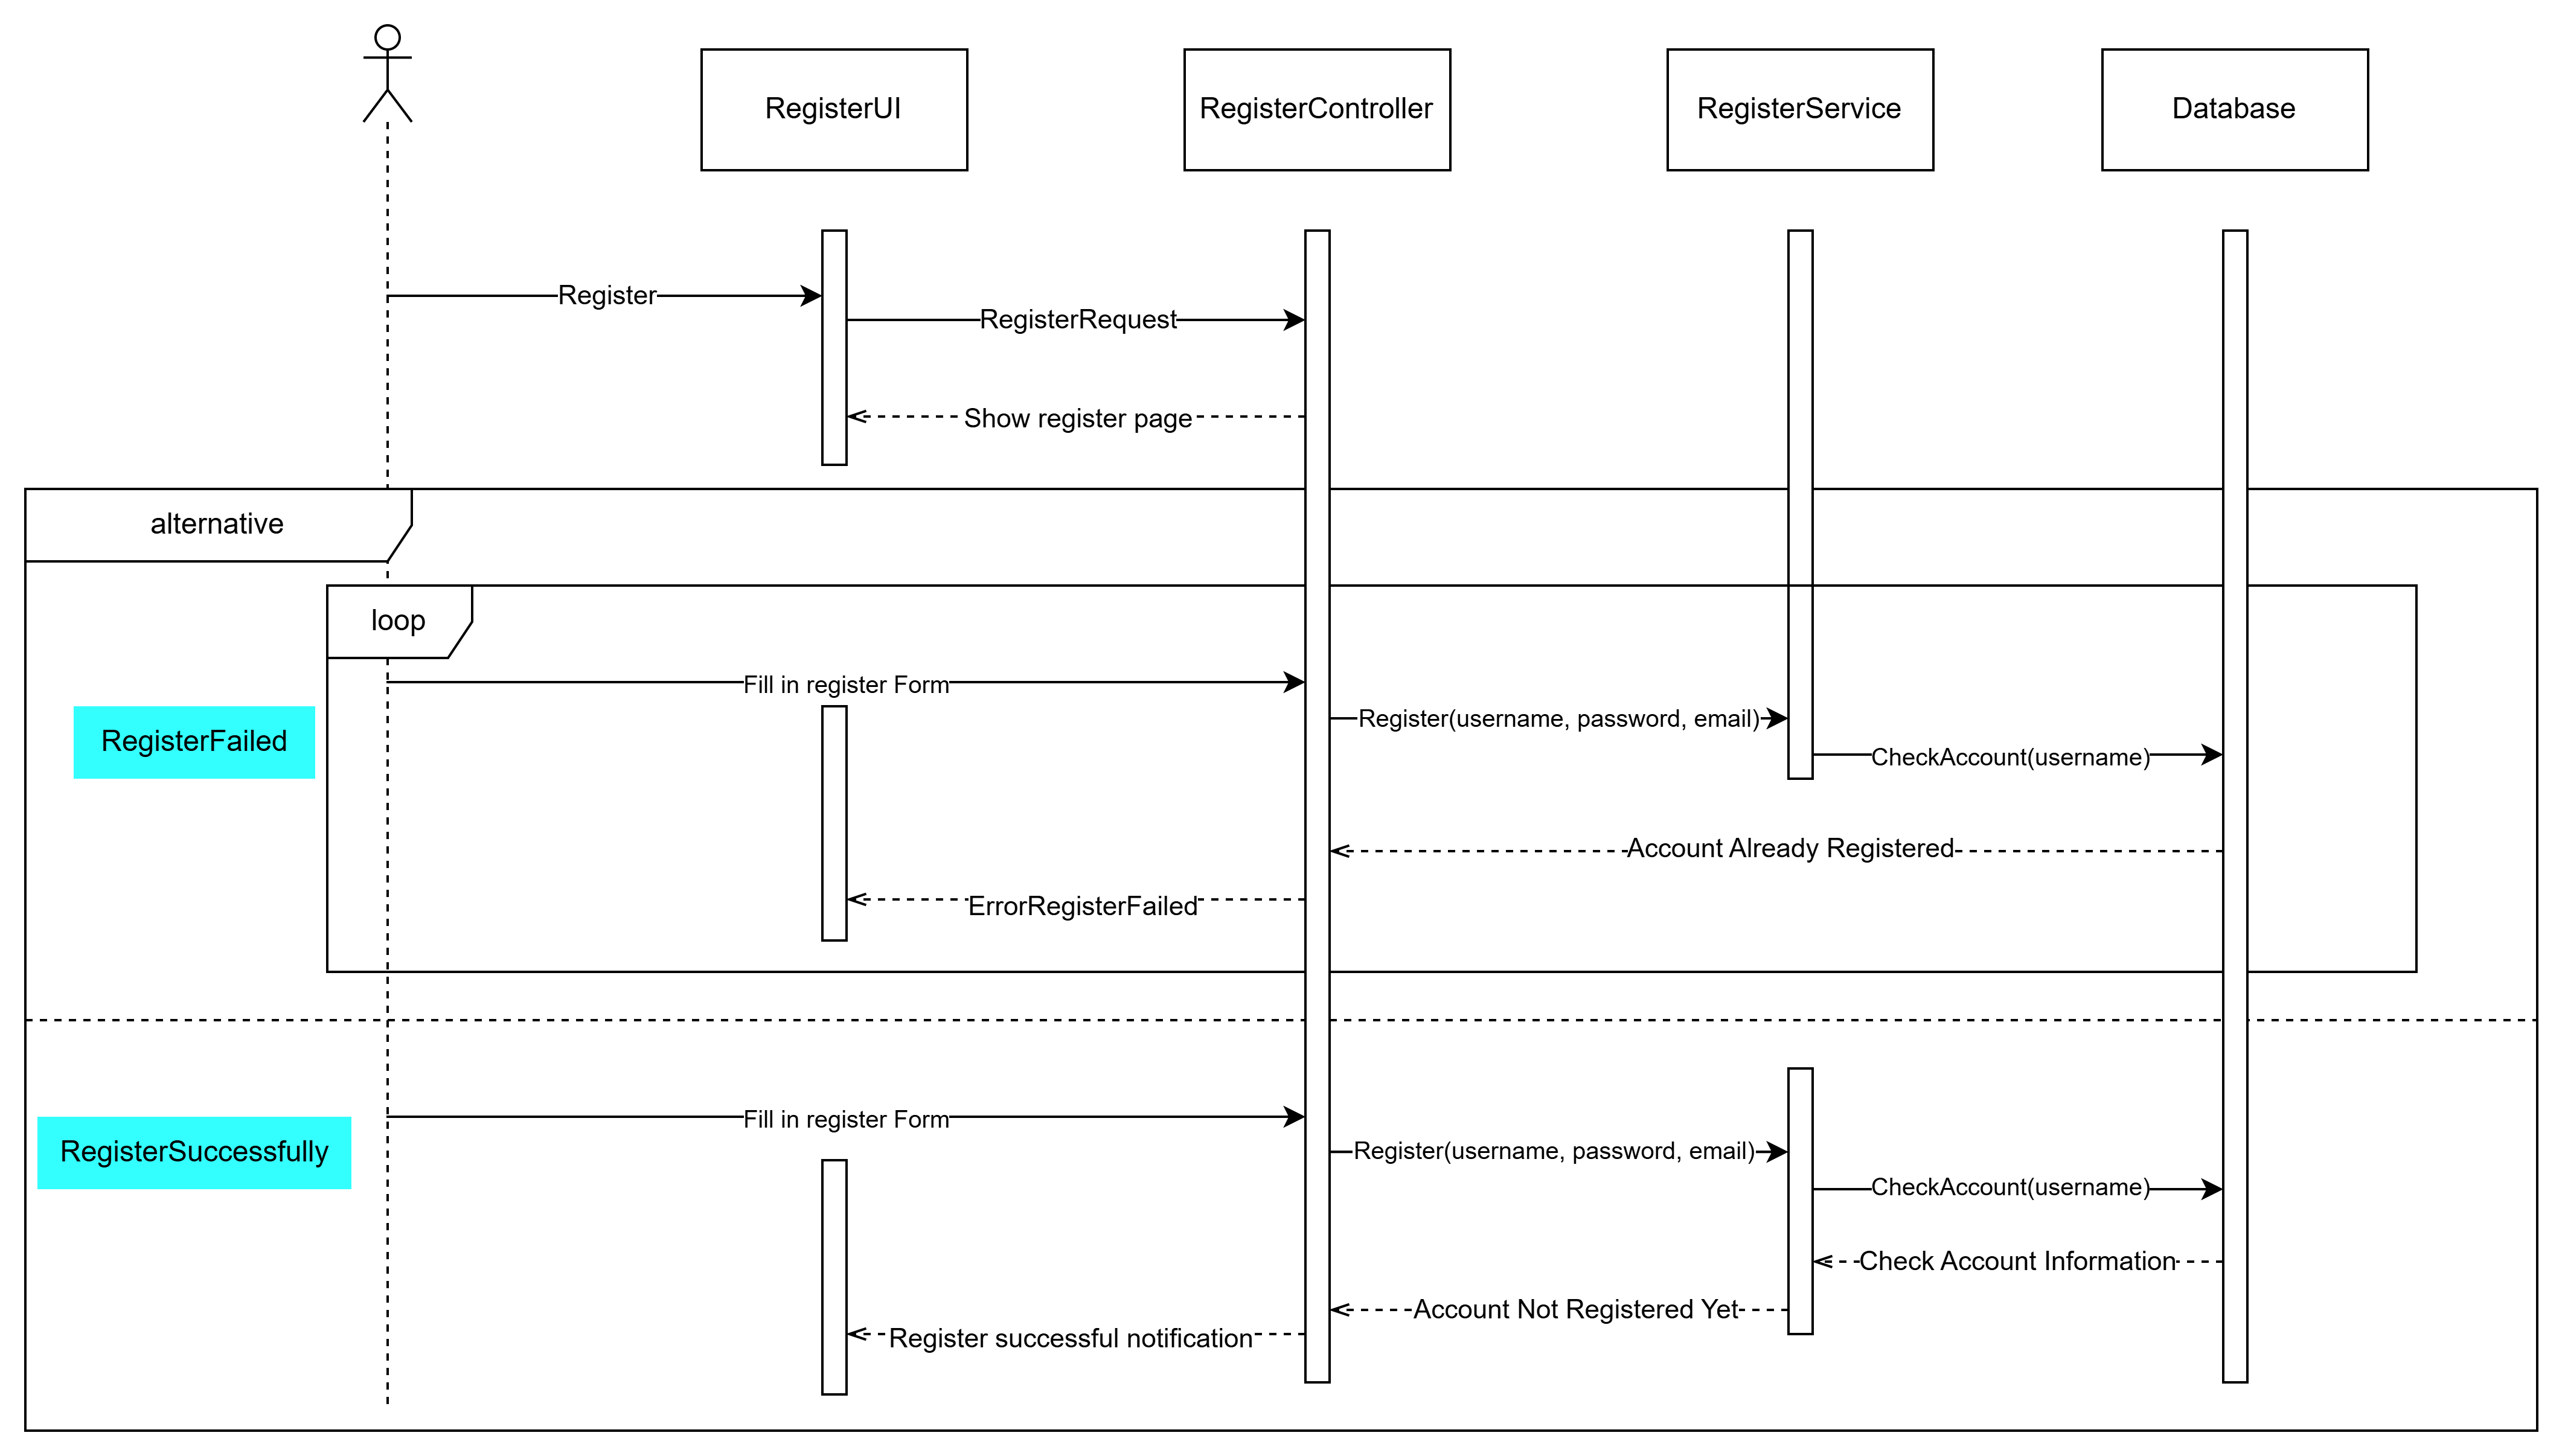
\includegraphics[scale=0.1]{img/Register_sequenceDiagram.png}
    \caption{Lược đồ tuần tự cho Đăng ký tài khoản}
	
\end{figure}

Khi người dùng chọn "Đăng ký tài khoản", người dùng sẽ được đưa đến trang "Đăng ký tài khoản". Ở đó sẽ chứa biểu mẫu yêu cầu người dùng điền vào để có thể tạo tài khoản thành công. Sau khi hoàn thành công việc điền biểu mẫu và yêu cầu tạo tài khoản, hệ thống sẽ kiểm tra thông tin tài khoản người dùng đã có trong cơ sở dữ liệu của hệ thống chưa? Nếu chưa có, hệ thống sẽ tạo tài khoản thành công, thông báo cho người dùng "Tạo tài khoản thành công" và chuyển hướng người dùng đến trang "Đăng nhập". Còn nếu tên tài khoản của người dùng đã có trong cơ sở dữ liệu, hệ thống sẽ thông báo cho người dùng "Tên tài khoản đã được sử dụng." và yêu cầu người dùng đổi tên tài khoản khác.

\subsection{Đăng nhập tài khoản }

\begin{figure}[H]

	\centering
    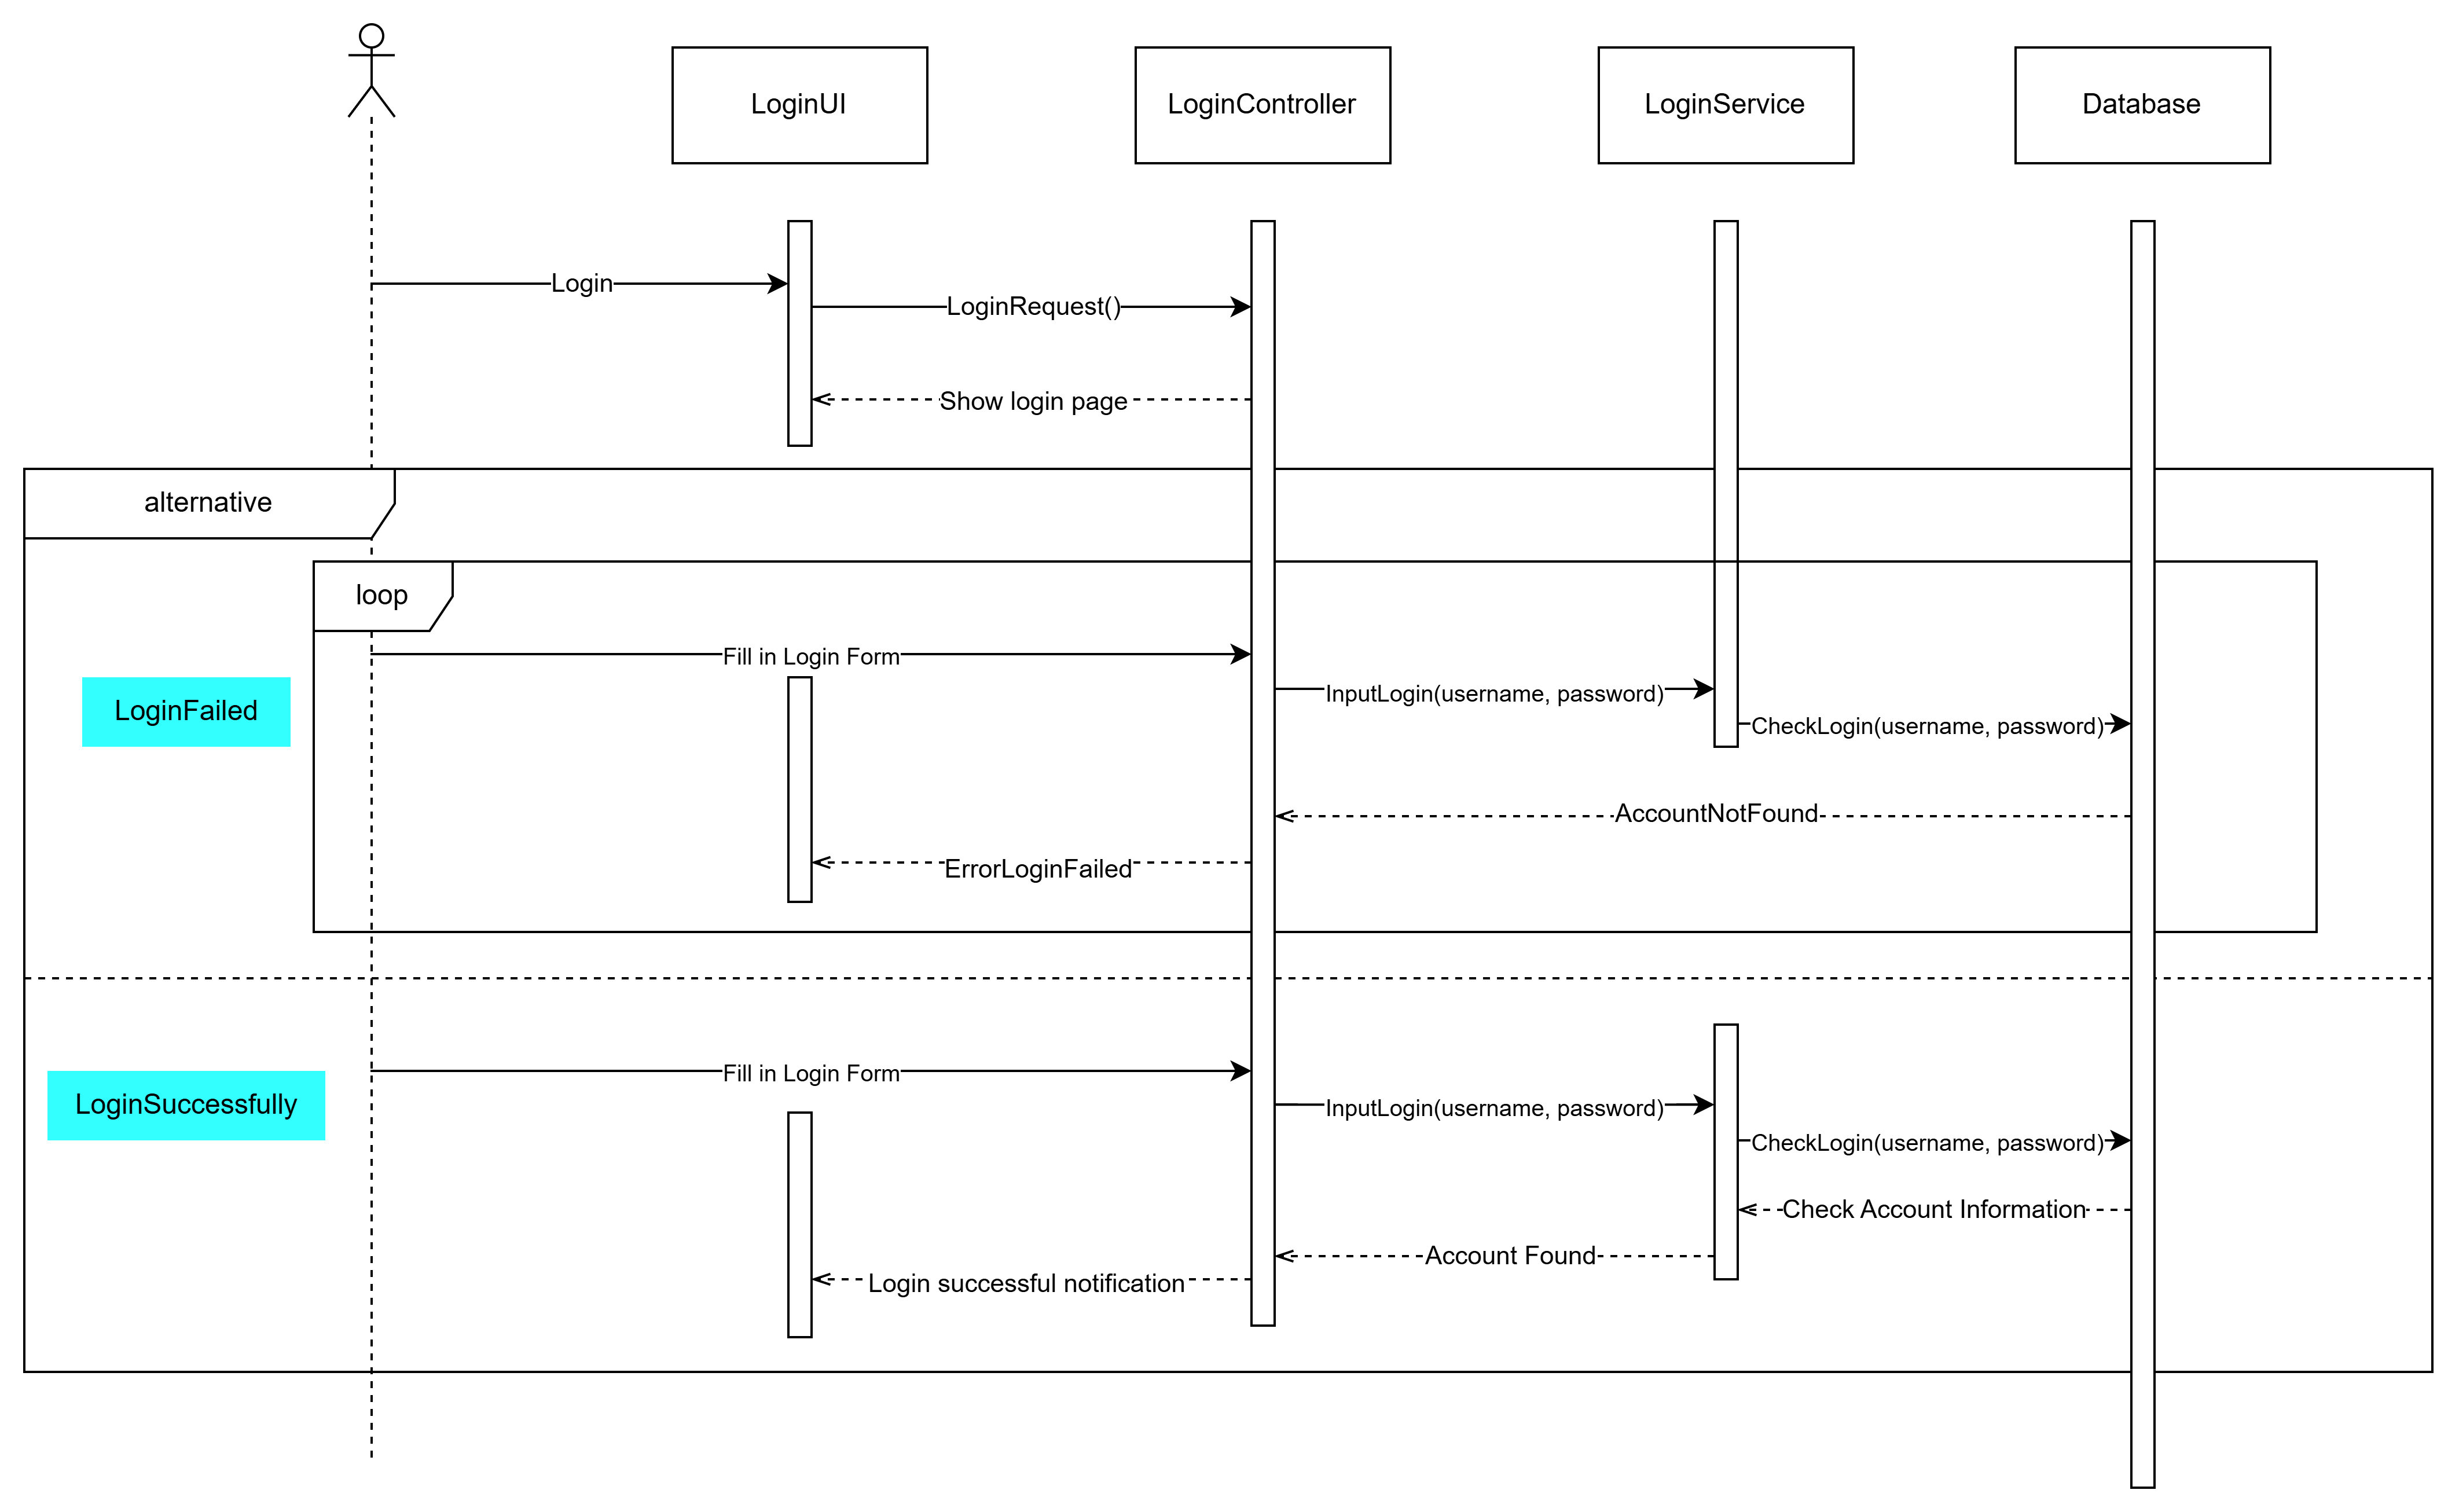
\includegraphics[scale=0.1]{img/Login_sequenceDiagram.png}
    \caption{Lược đồ tuần tự cho Đăng nhập tài khoản}
	
\end{figure}

Sơ đồ thể hiện cho quá trình đăng nhập tài khoản chung đối với nhiều vai trò người dùng khác nhau. Trong quá trình này, khi người dùng chọn phần "Đăng nhập", hệ thống sẽ chuyển hướng người dùng đến đường link của trang "Đăng nhập tài khoản". Trang web sẽ hiển thị một trang biểu mẫu cho người dùng điền tài khoản và mật khẩu. 

Sau khi người dùng điền thông tin tài khoản và mật khẩu vào biểu mẫu. Hệ thống sẽ kiểm tra thông tin tài khoản và mật khẩu mà người dùng điền vào có khớp với dữ liệu của hệ thống không? Nếu khớp, hệ thống sẽ thông báo người dùng đăng nhập thành công và chuyển hướng người dùng đến trang chủ. Nếu không khớp với dữ liệu của hệ thống, hệ thống sẽ thông báo cho người dùng "Đăng nhập thất bại" và chỉ người dùng tài khoản hay mật khẩu của người dùng bị sai.

\subsection{Quản lý CV}


\begin{figure}[H]

	\centering
    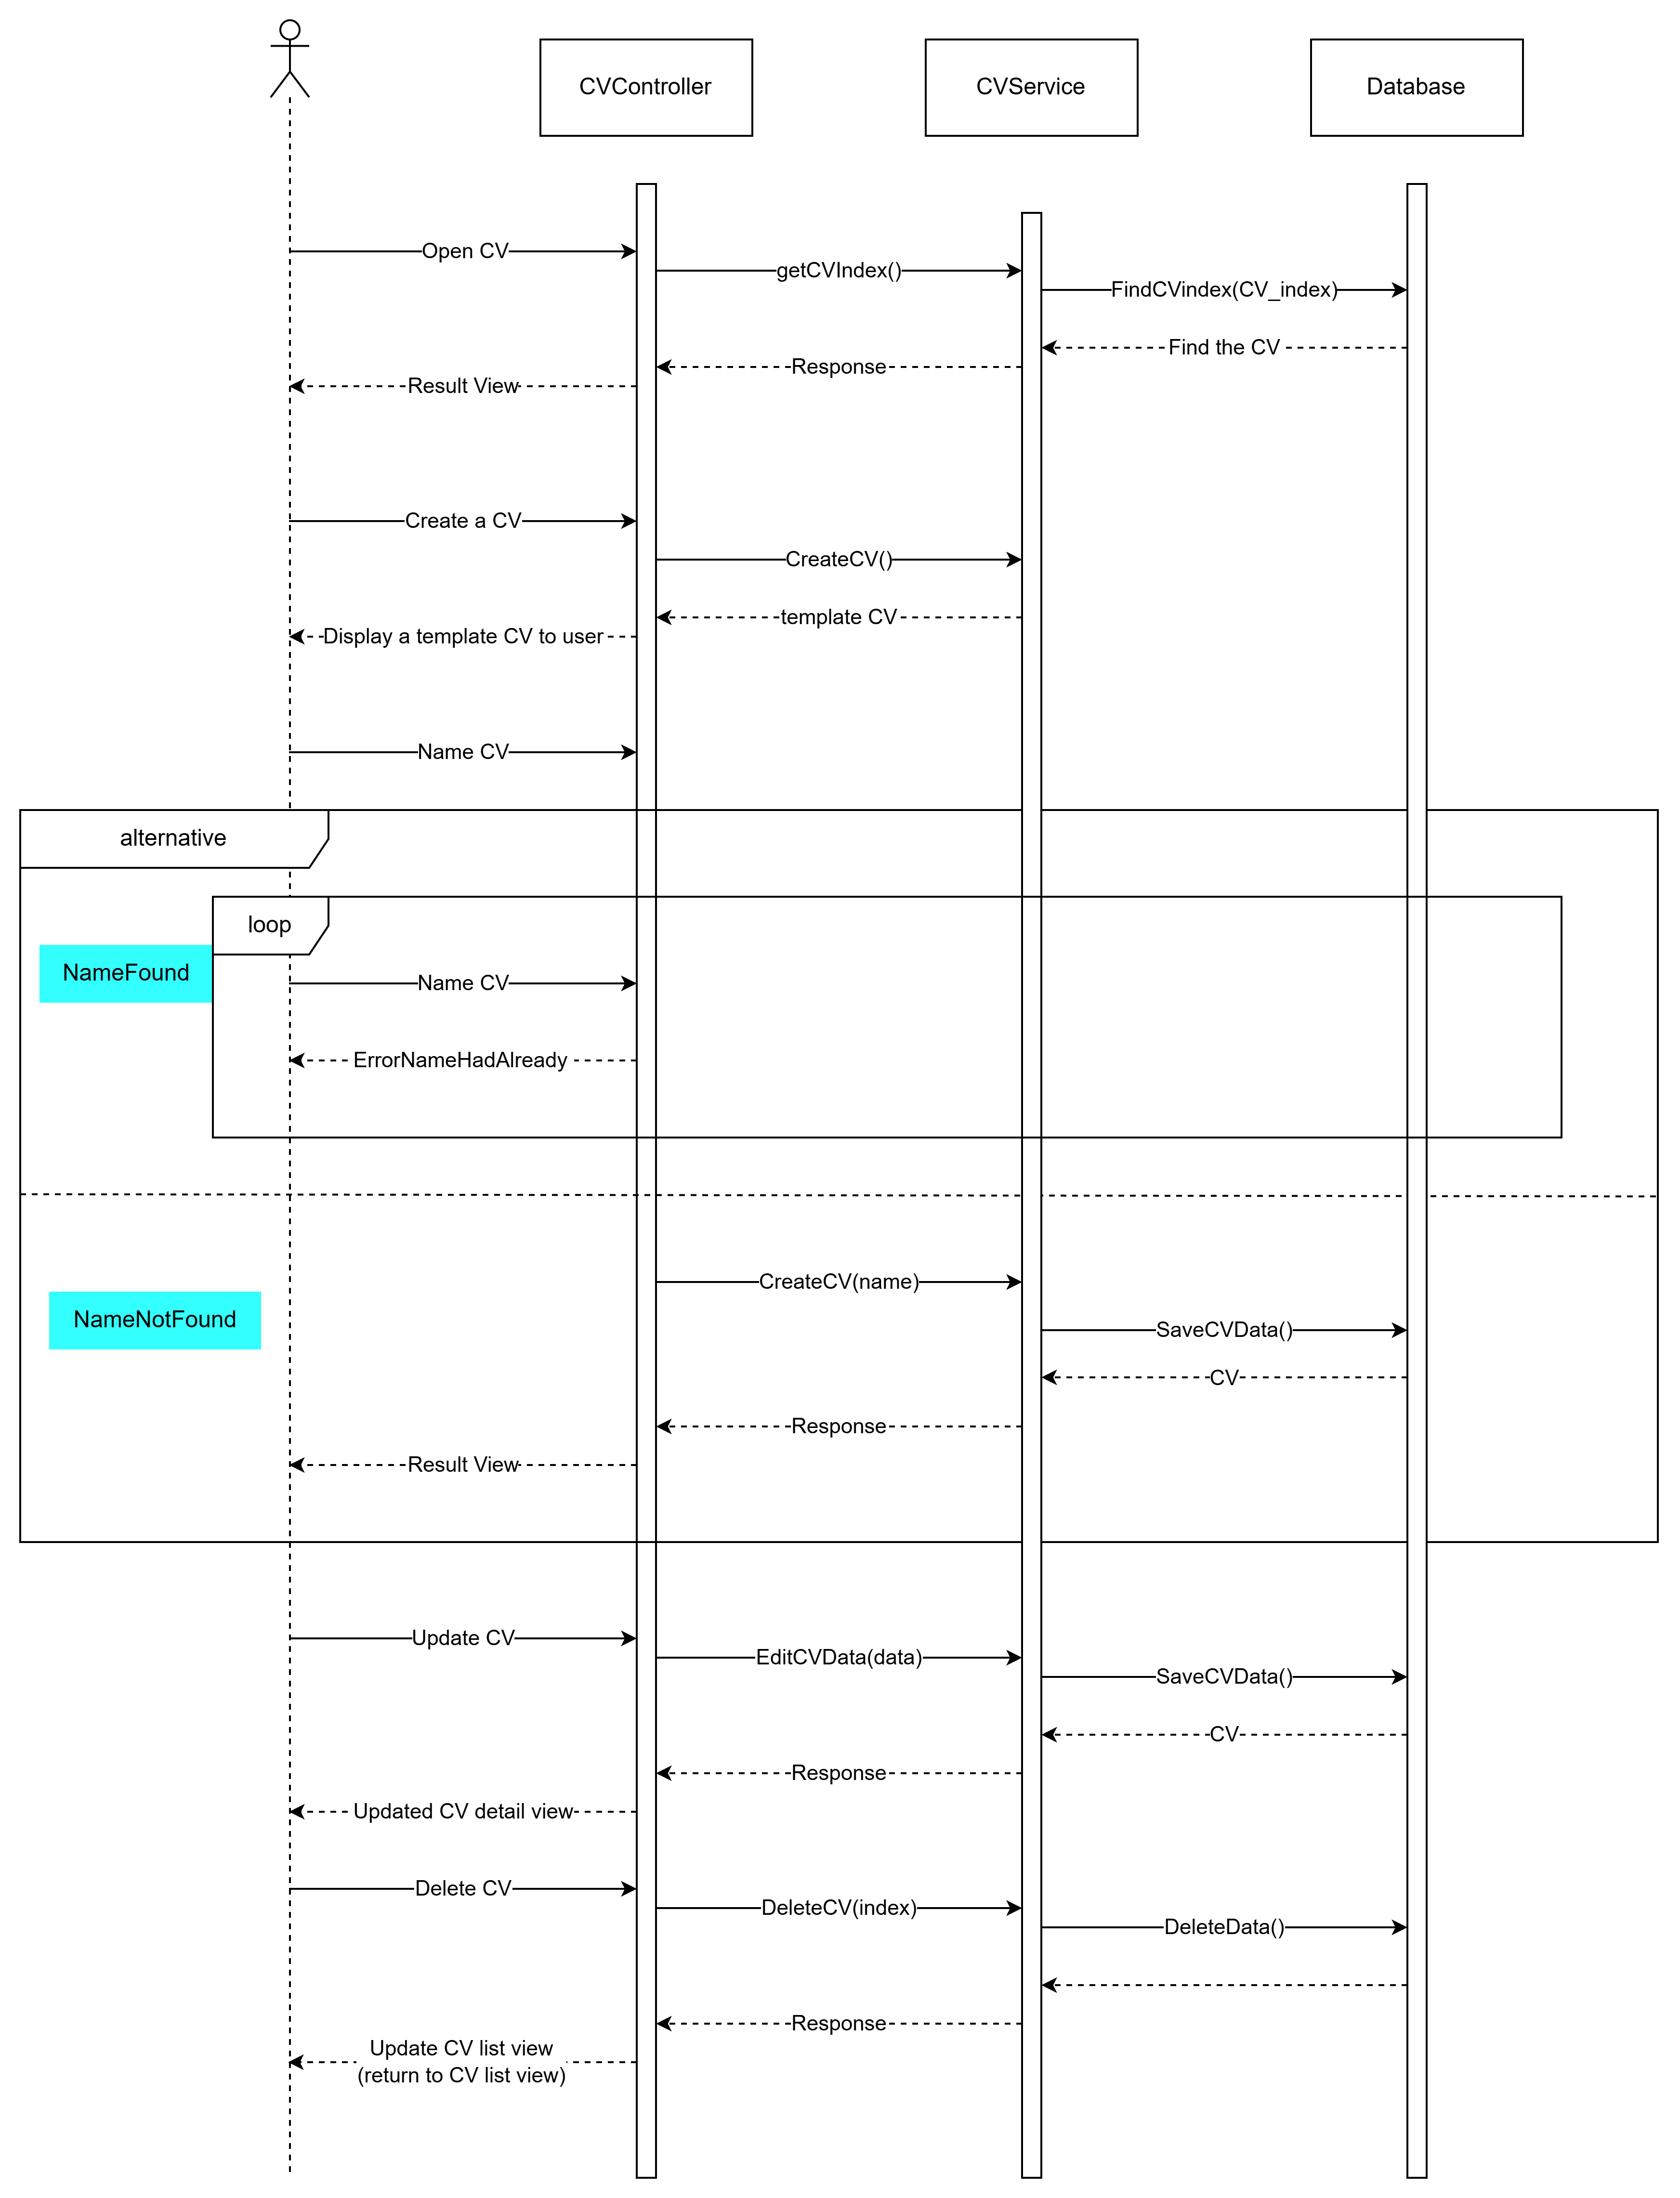
\includegraphics[scale = 0.1]{img/CV_Management_sequenceDiagram.png}
    \caption{Lược đồ tuần tự cho Quản lý CV}
	
\end{figure}

Khi người dùng vào trang "Quản lý CV", hệ thống sẽ lấy danh sách những bản CV mà người dùng đã tạo trước đó và hiển thị lên trang web. Người dùng có thể chọn chức năng "Tạo CV" để tạo thêm CV cho chính mình. Khi đó, hệ thống sẽ hiển thị một bản CV mẫu lên trang web, nhưng bản CV đó chỉ là bản nháp và nếu người dùng không lưu hay đặt tên cho bản CV, lúc thoát ra, hệ thống sẽ không lưu dữ liệu của bản CV nháp đó vào cơ sở dữ liệu của hệ thống. Còn khi đặt tên cho CV, hệ thống sẽ kiểm tra tên CV của bạn liệu có trùng tên với những CV khác của mình. Nếu có, hệ thống sẽ thông báo "Tên này đã được sử dụng. Vui lòng sử dụng tên khác". Ngược lại, nếu không trùng thì hệ thống sẽ thông báo "Lưu CV thành công".

Người dùng cũngcó thể  chọn một bản CV trong danh sách và chọn thực hiện xoá hoặc sửa CV, hệ thống sẽ lấy ID của CV vừa chọn và lấy toàn bộ thông tin của bản CV đó. Nếu người dùng chọn xoá CV, hệ thống sẽ xoá hoàn toàn dữ liệu của bản CV đó ra khỏi cơ sở dữ liệu của hệ thống. Còn nếu người dùng chọn sửa CV, hệ thống sẽ hiển thị thông tin dữ liệu của bản CV lên trang web của người dùng. Và ở đây người dùng có thể tự mình chỉnh sửa CV của mình theo ý mình muốn.


\subsection{Ứng tuyển công việc}

\begin{figure}[H]

	\centering
    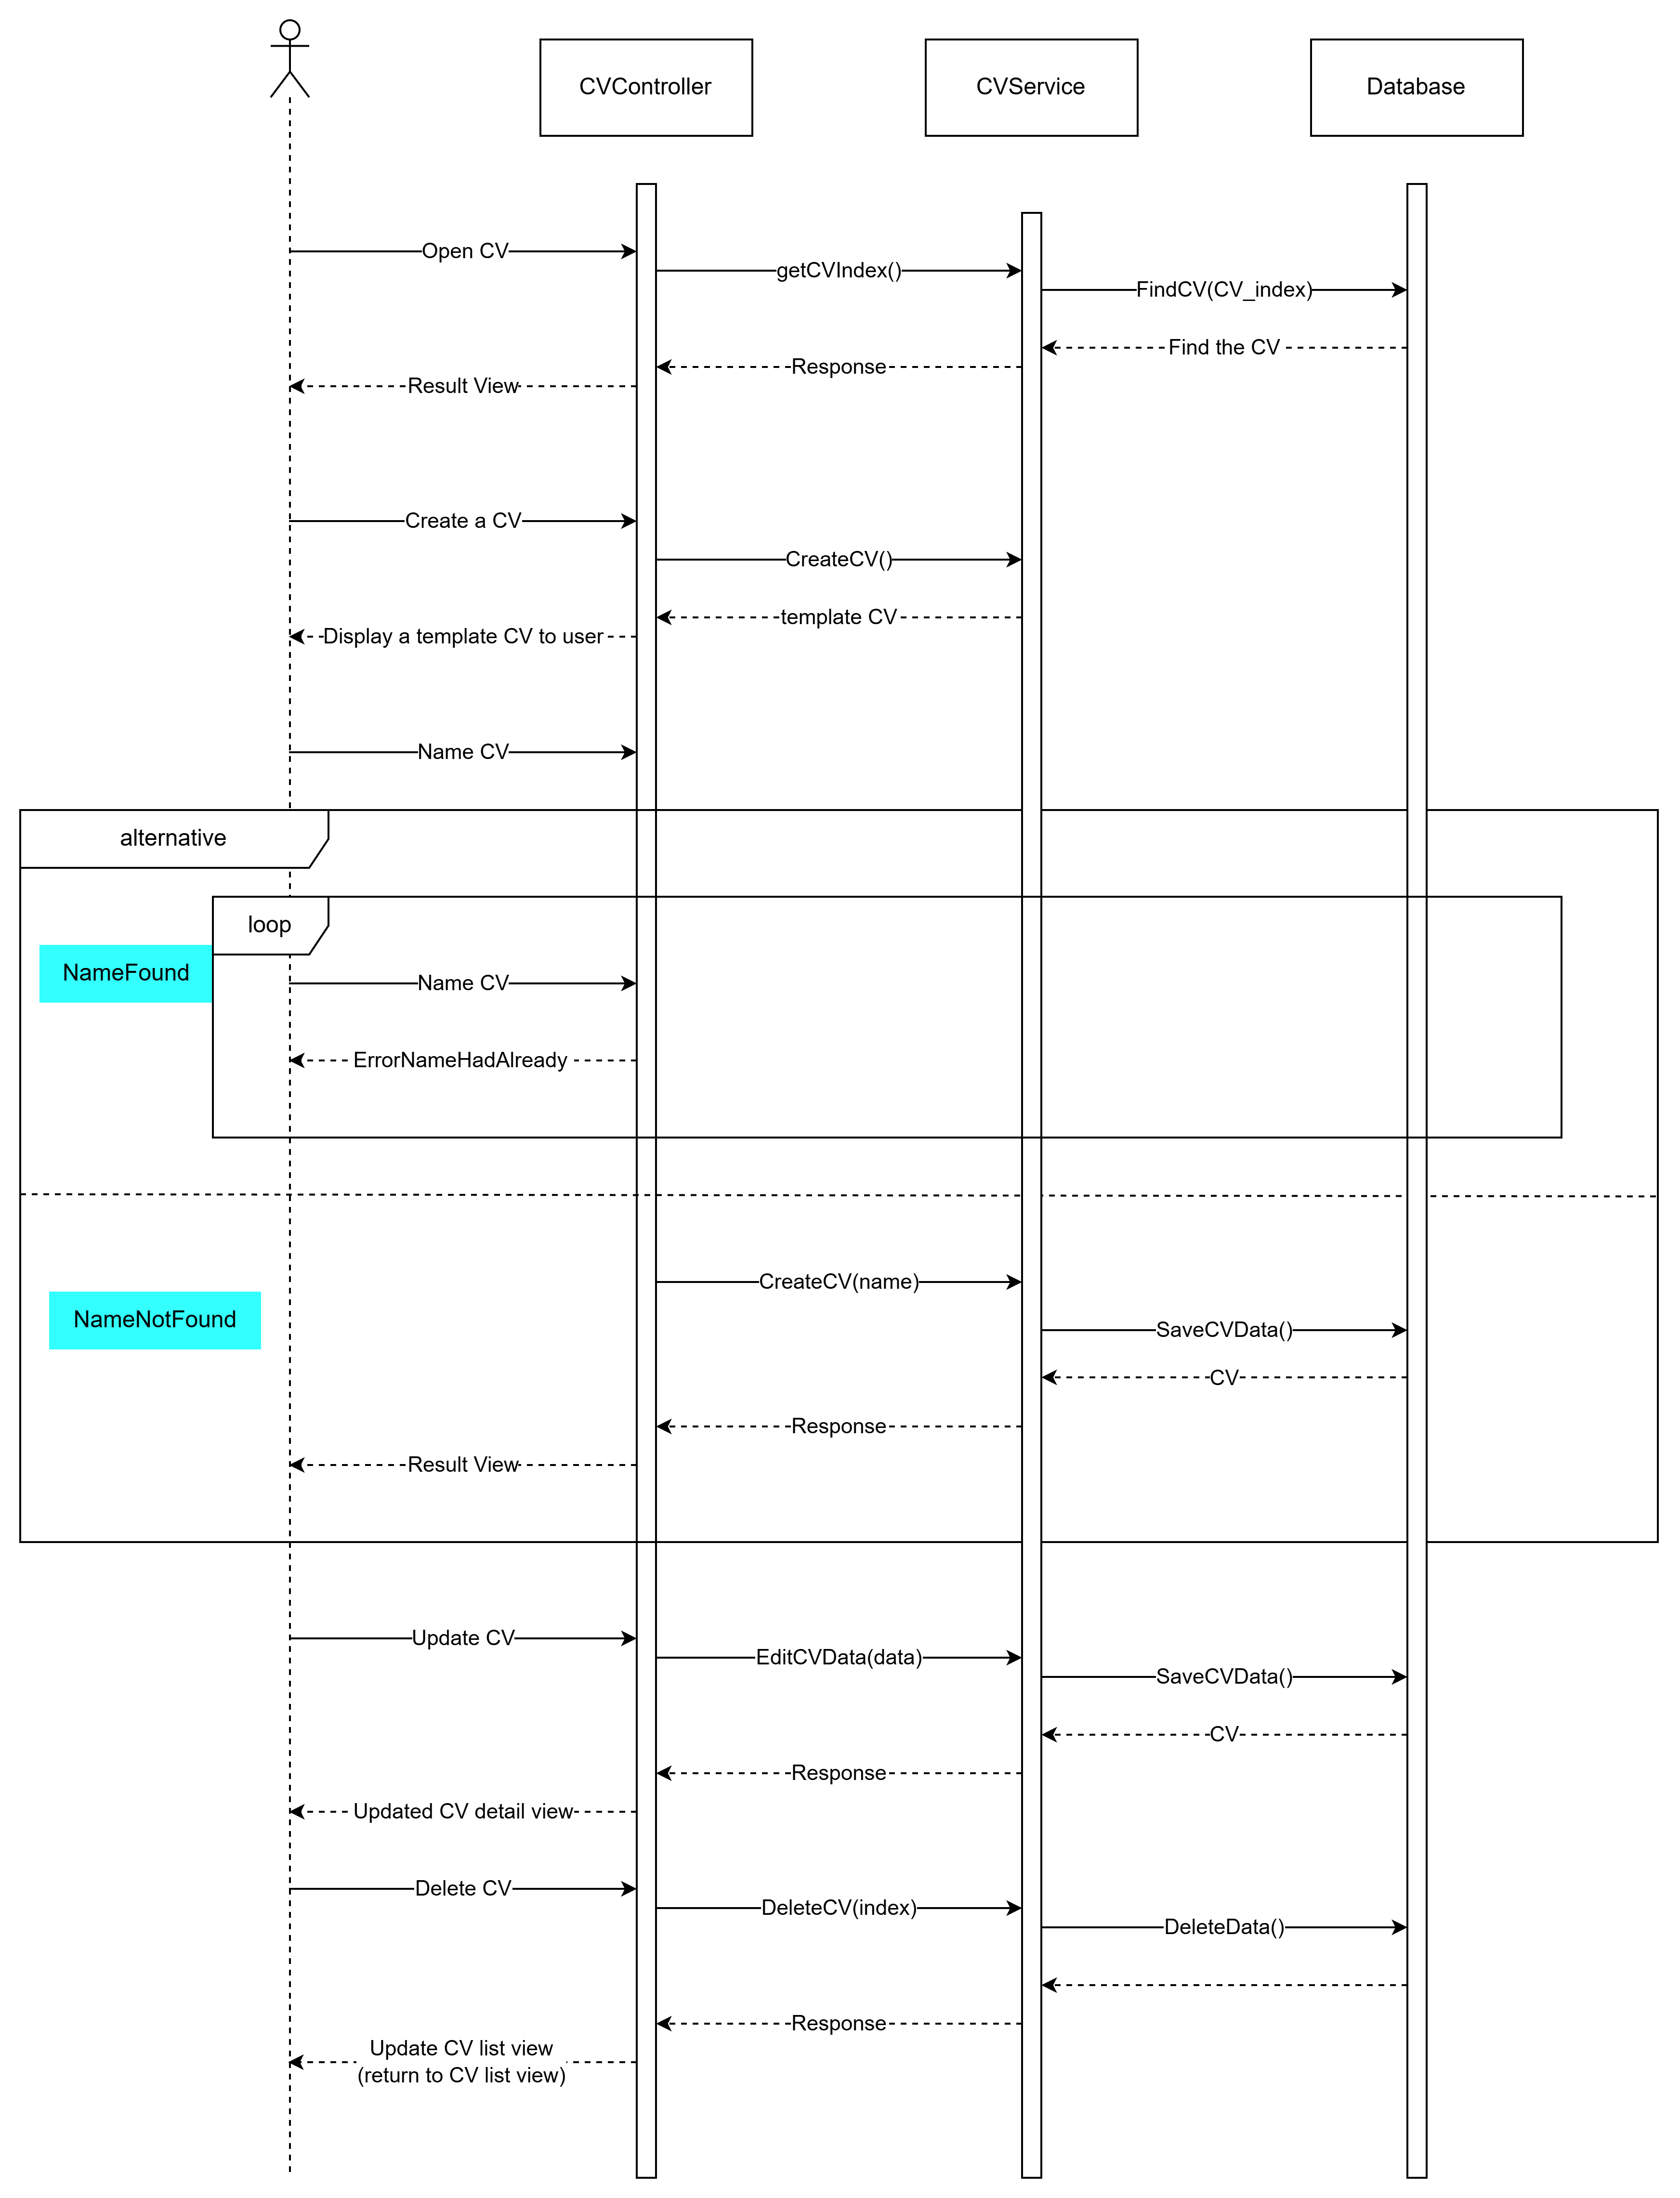
\includegraphics[scale = 0.1]{img/ApplyJob_sequenceDiagram.png}
    \caption{Lược đồ tuần tự cho Ứng tuyển công việc}
	
\end{figure}

Sơ đồ tuần tự ở trên thể hiện quy trình làm việc của một ứng viên khi ứng tuyển vào một vị trí công việc của một bài đăng tuyển dụng. Khi người dùng vào trang "Tìm kiếm việc làm", hệ thống lấy từng danh sách bài đăng tuyển dụng nhân sự và hiển thị chúng lên trang web. Mỗi bài đăng sẽ có những thông tin ngắn gọn về nội dung của bài đăng và cũng như tên công ty muốn tuyển dụng. Người dùng sẽ chọn một trong số chúng và hệ thống sẽ hiển thị toàn bộ thông tin nội dung của bài đăng.

Người sẽ đọc và nếu cảm thấy thông tin tuyển dụng thực sự phù hợp với mình, họ có thể ứng tuyển vào vị trí công việc đó của công việc. Nếu không, họ có thể chọn lựa một bài đăng khác phù hợp với tiêu chí của mình. Khi người dùng ứng tuyển vào một vị trí công việc của công ty, hệ thống sẽ kiểm tra tài khoản người dùng liệu đã có một bản CV đang trong trạng thái ứng tuyển hay chưa. Nếu chưa, hệ thống sẽ thông báo cho người dùng "Bạn vẫn chưa có CV để ứng tuyển công việc" và người dùng có thể lựa chọn hoặc ở lại trang "Tìm kiếm công việc" hoặc chuyển hướng tới trang "Quản lý CV". Sau khi chuyển hướng tới trang "Quản lý CV", người có thể tự tạo cho mình một bản CV mới hoặc có thể upload một bản CV sẵn có của mình lên trang web và đặt trạng thái CV của mình là "Ứng tuyển".

Sau cùng, người dùng sẽ được thông báo "Ứng tuyển thành công" và hệ thống sẽ gửi CV của người dùng đến công ty ứng tuyển.

\section{Thiết kế cơ sở dữ liệu}

\subsection{Thiết kế sơ đồ thực thể (ERD)}
Để thiết kế cơ sở dữ liệu, tôi đã sử dụng sơ đồ thực thể (Entity-Relationship Diagram - ERD) để trong việc thiết kế cơ sở dữ liệu để biểu diễn các thực thể trong hệ thống và mối quan hệ, tương tác giữa chúng.

\begin{figure}[H]

	\centering
    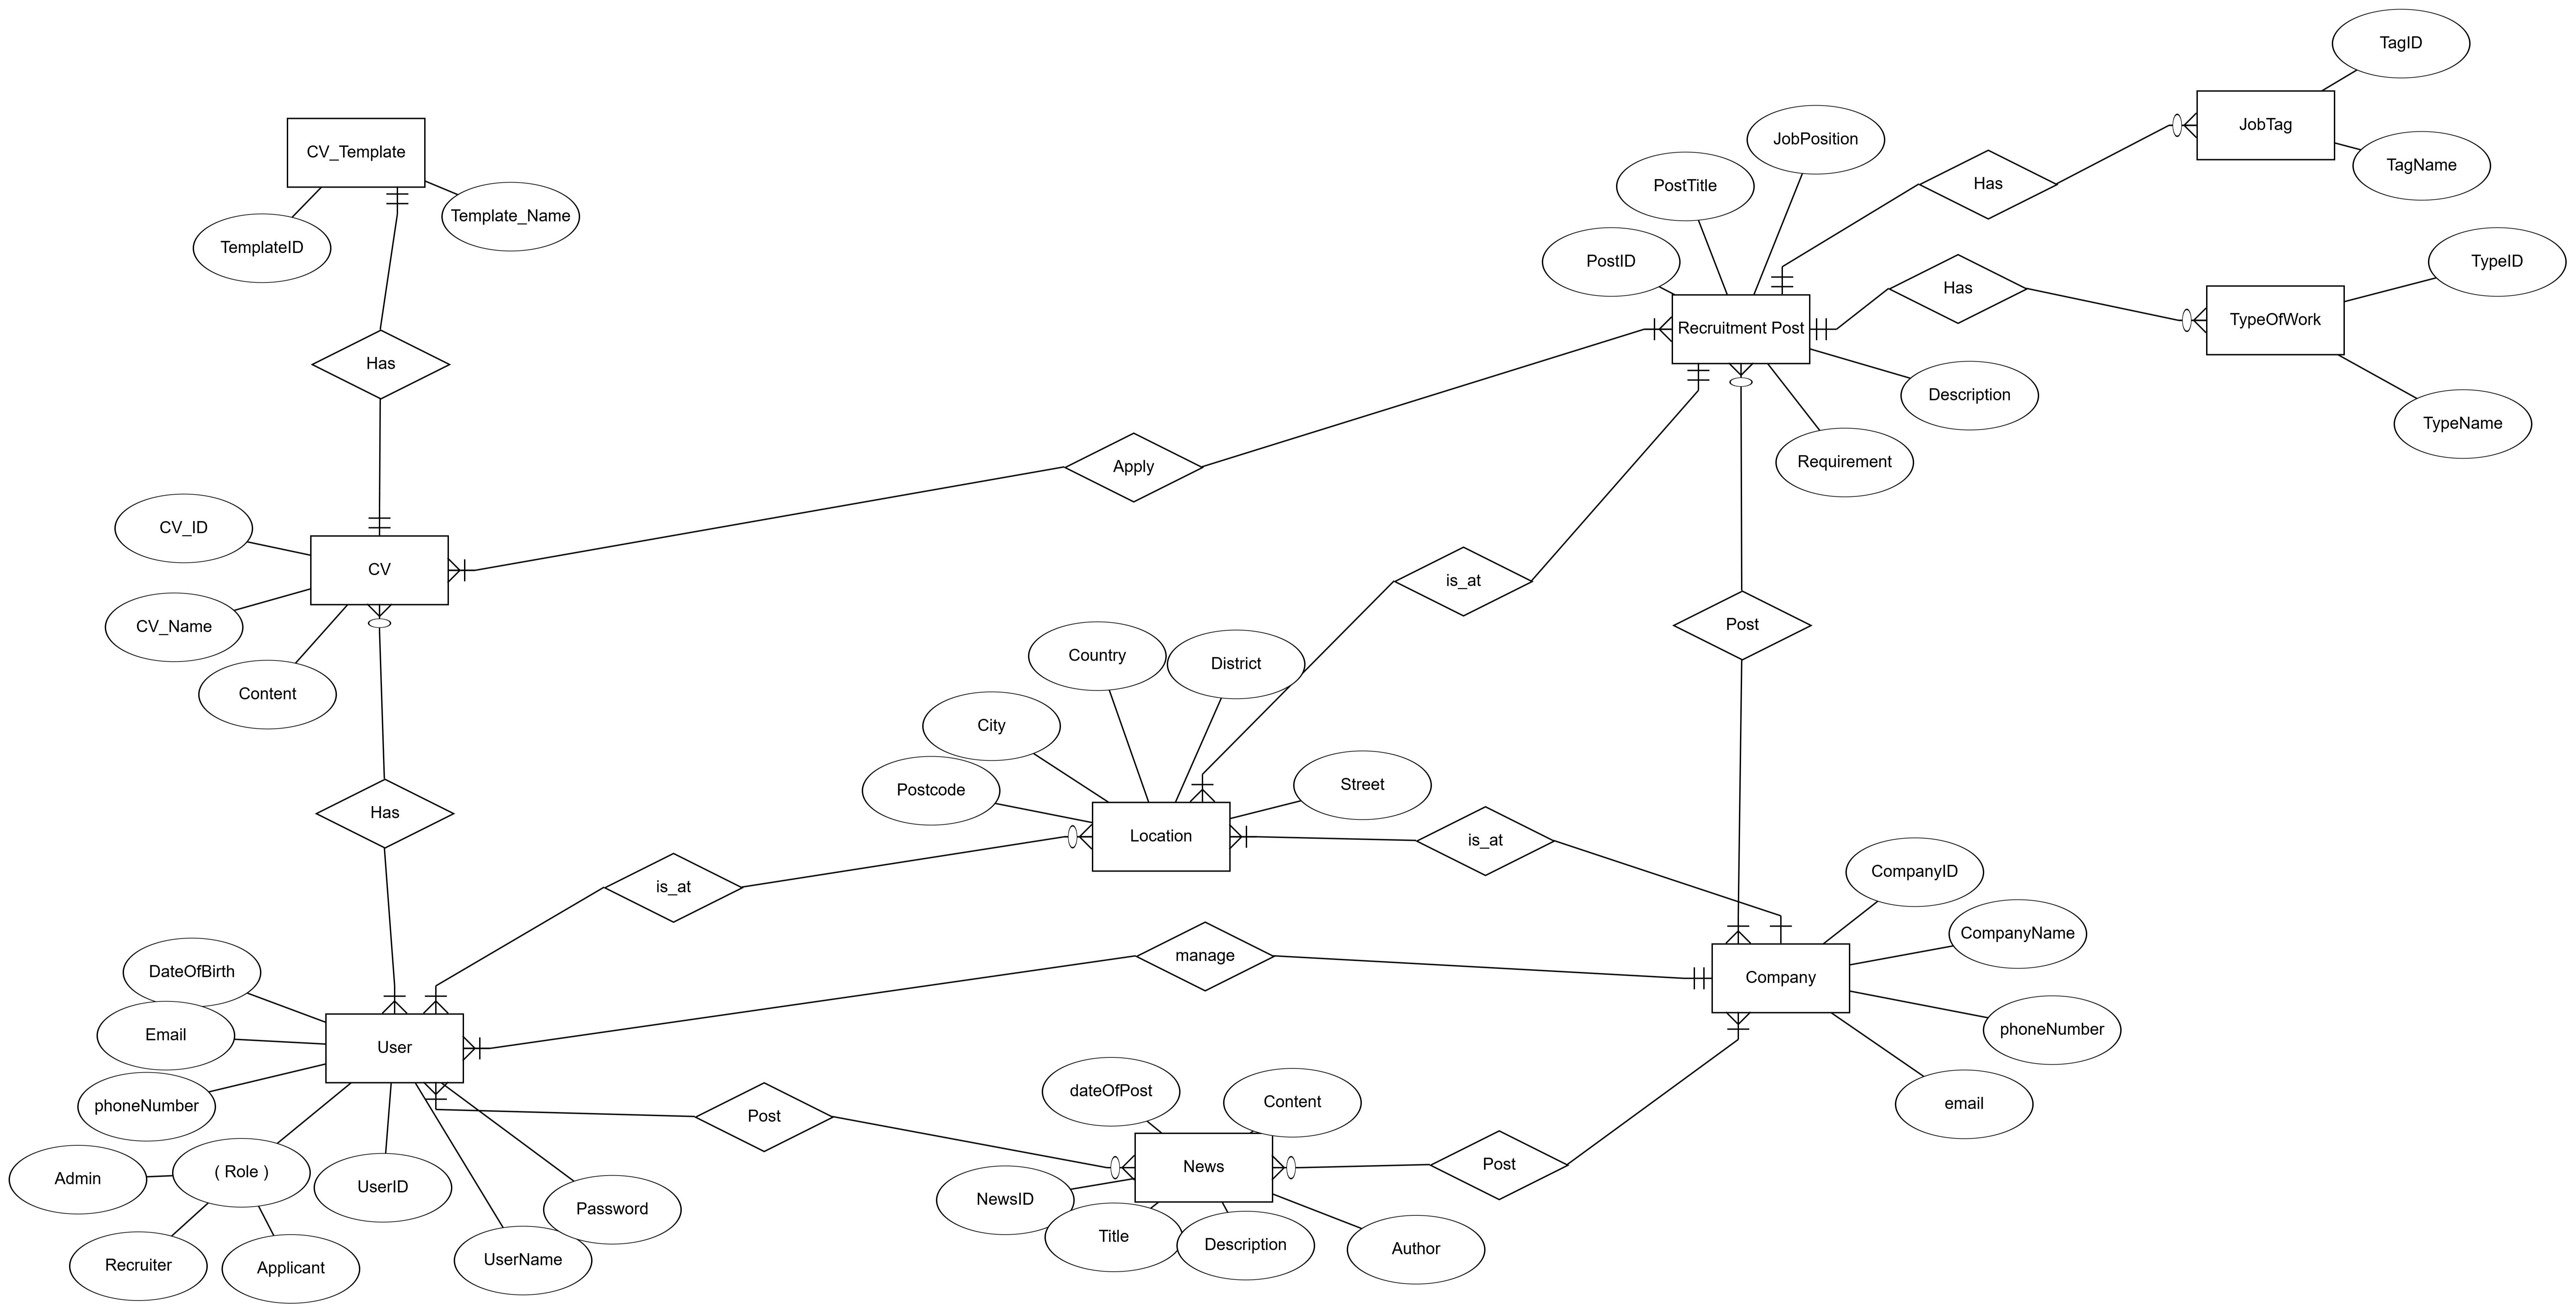
\includegraphics[angle=90,scale=0.08]{img/ERD.png}
    \caption{Sơ đồ thực thể (ERD)}
	
\end{figure}

Dưới đây là những thực thể có trong cơ sở dữ liệu của tôi:

\begin{itemize}
    \item \textbf{User:} đại diện cho các kiểu người dùng trên trang web. Nó chứa các thông tin cơ bản của người dùng và có thể thực hiện các chức năng của trang web.
    \item \textbf{Role:} đại diện cho các vai trò của người, gồm 3 role chính là: admin, applicant, recruiter/company.  Nó có thể thực hiện các chức năng cơ bản của người dùng chung. Tuy nhiên, đối với những vai trò đặc biệt như admin hay company, họ sẽ có các chức năng đặc biệt khác. VD: Đối với admin, họ có chức năng ban những users khác hay kiểm duyệt các bài đăng lên trang web,.... Hay với những doanh nghiệp (company) họ có thể thực hiện đăng những bài đăng tuyển dụng nhân viên lên trang web.
    \item \textbf{News:} là nơi chứa những thông tin, nội dung của những bản tin có trên trang web. Nó được viết và đăng lên bởi bất kỳ người dùng nào. Nhưng để được lên trang web thì cần phải được admin của trang web xét duyệt.
    \item \textbf{Recruitment Post:} là nơi chứa những thông tin, nội dung của những bài đăng tuyển dụng nhân sự của các công ty, doanh nghiệp. Nó đăng được đăng bởi doanh nghiệp, công ty. Nhưng cũng giống như tin tức (news), để lên được trang web, cần phải thông qua sự xét duyệt của admin.
    \item \textbf{CV:} là danh sách các bản CV của người dùng. Nó bao gồm: nội dung, tiêu đề, .... Mỗi CV đều có một template cho riêng mình. Tuy nhiên cũng có một bản CV custom không thuộc bất kỳ một template nào cả. Và nếu upload 1 bản CV lên trang web, hệ thông sẽ xem bản CV dưới dạng dữ liệu là file và không thể chỉnh sửa được.
    \item \textbf{CV Template:} gồm nhiều mẫu CV khác nhau phù hợp nhiều chủ đề và ngành nghề khác nhau.
    \item \textbf{Location:} đại diện cho địa chỉ của người và công ty. Đối với công ty, sẽ có nhiều địa chỉ khác nhau như: địa chỉ cơ sở chính, chi nhánh,....
    \item \textbf{Job Tag:} bao gồm các đối tượng ngành nghề mà doanh nghiệp muốn hướng đến. VD như: marketing, IT, phục vụ,... 
    \item \textbf{Type of work:} bao gồm các thể loại công việc. Nó thể hiện loại công việc, kinh nghiệm, vị trí mà công ty muốn tuyển dụng như part-time, full-time, night-shift, intern, fresher, senior,....
\end{itemize}


\subsection{Lược đồ quan hệ (Relational Schema) }

\begin{figure}[H]

	\centering
    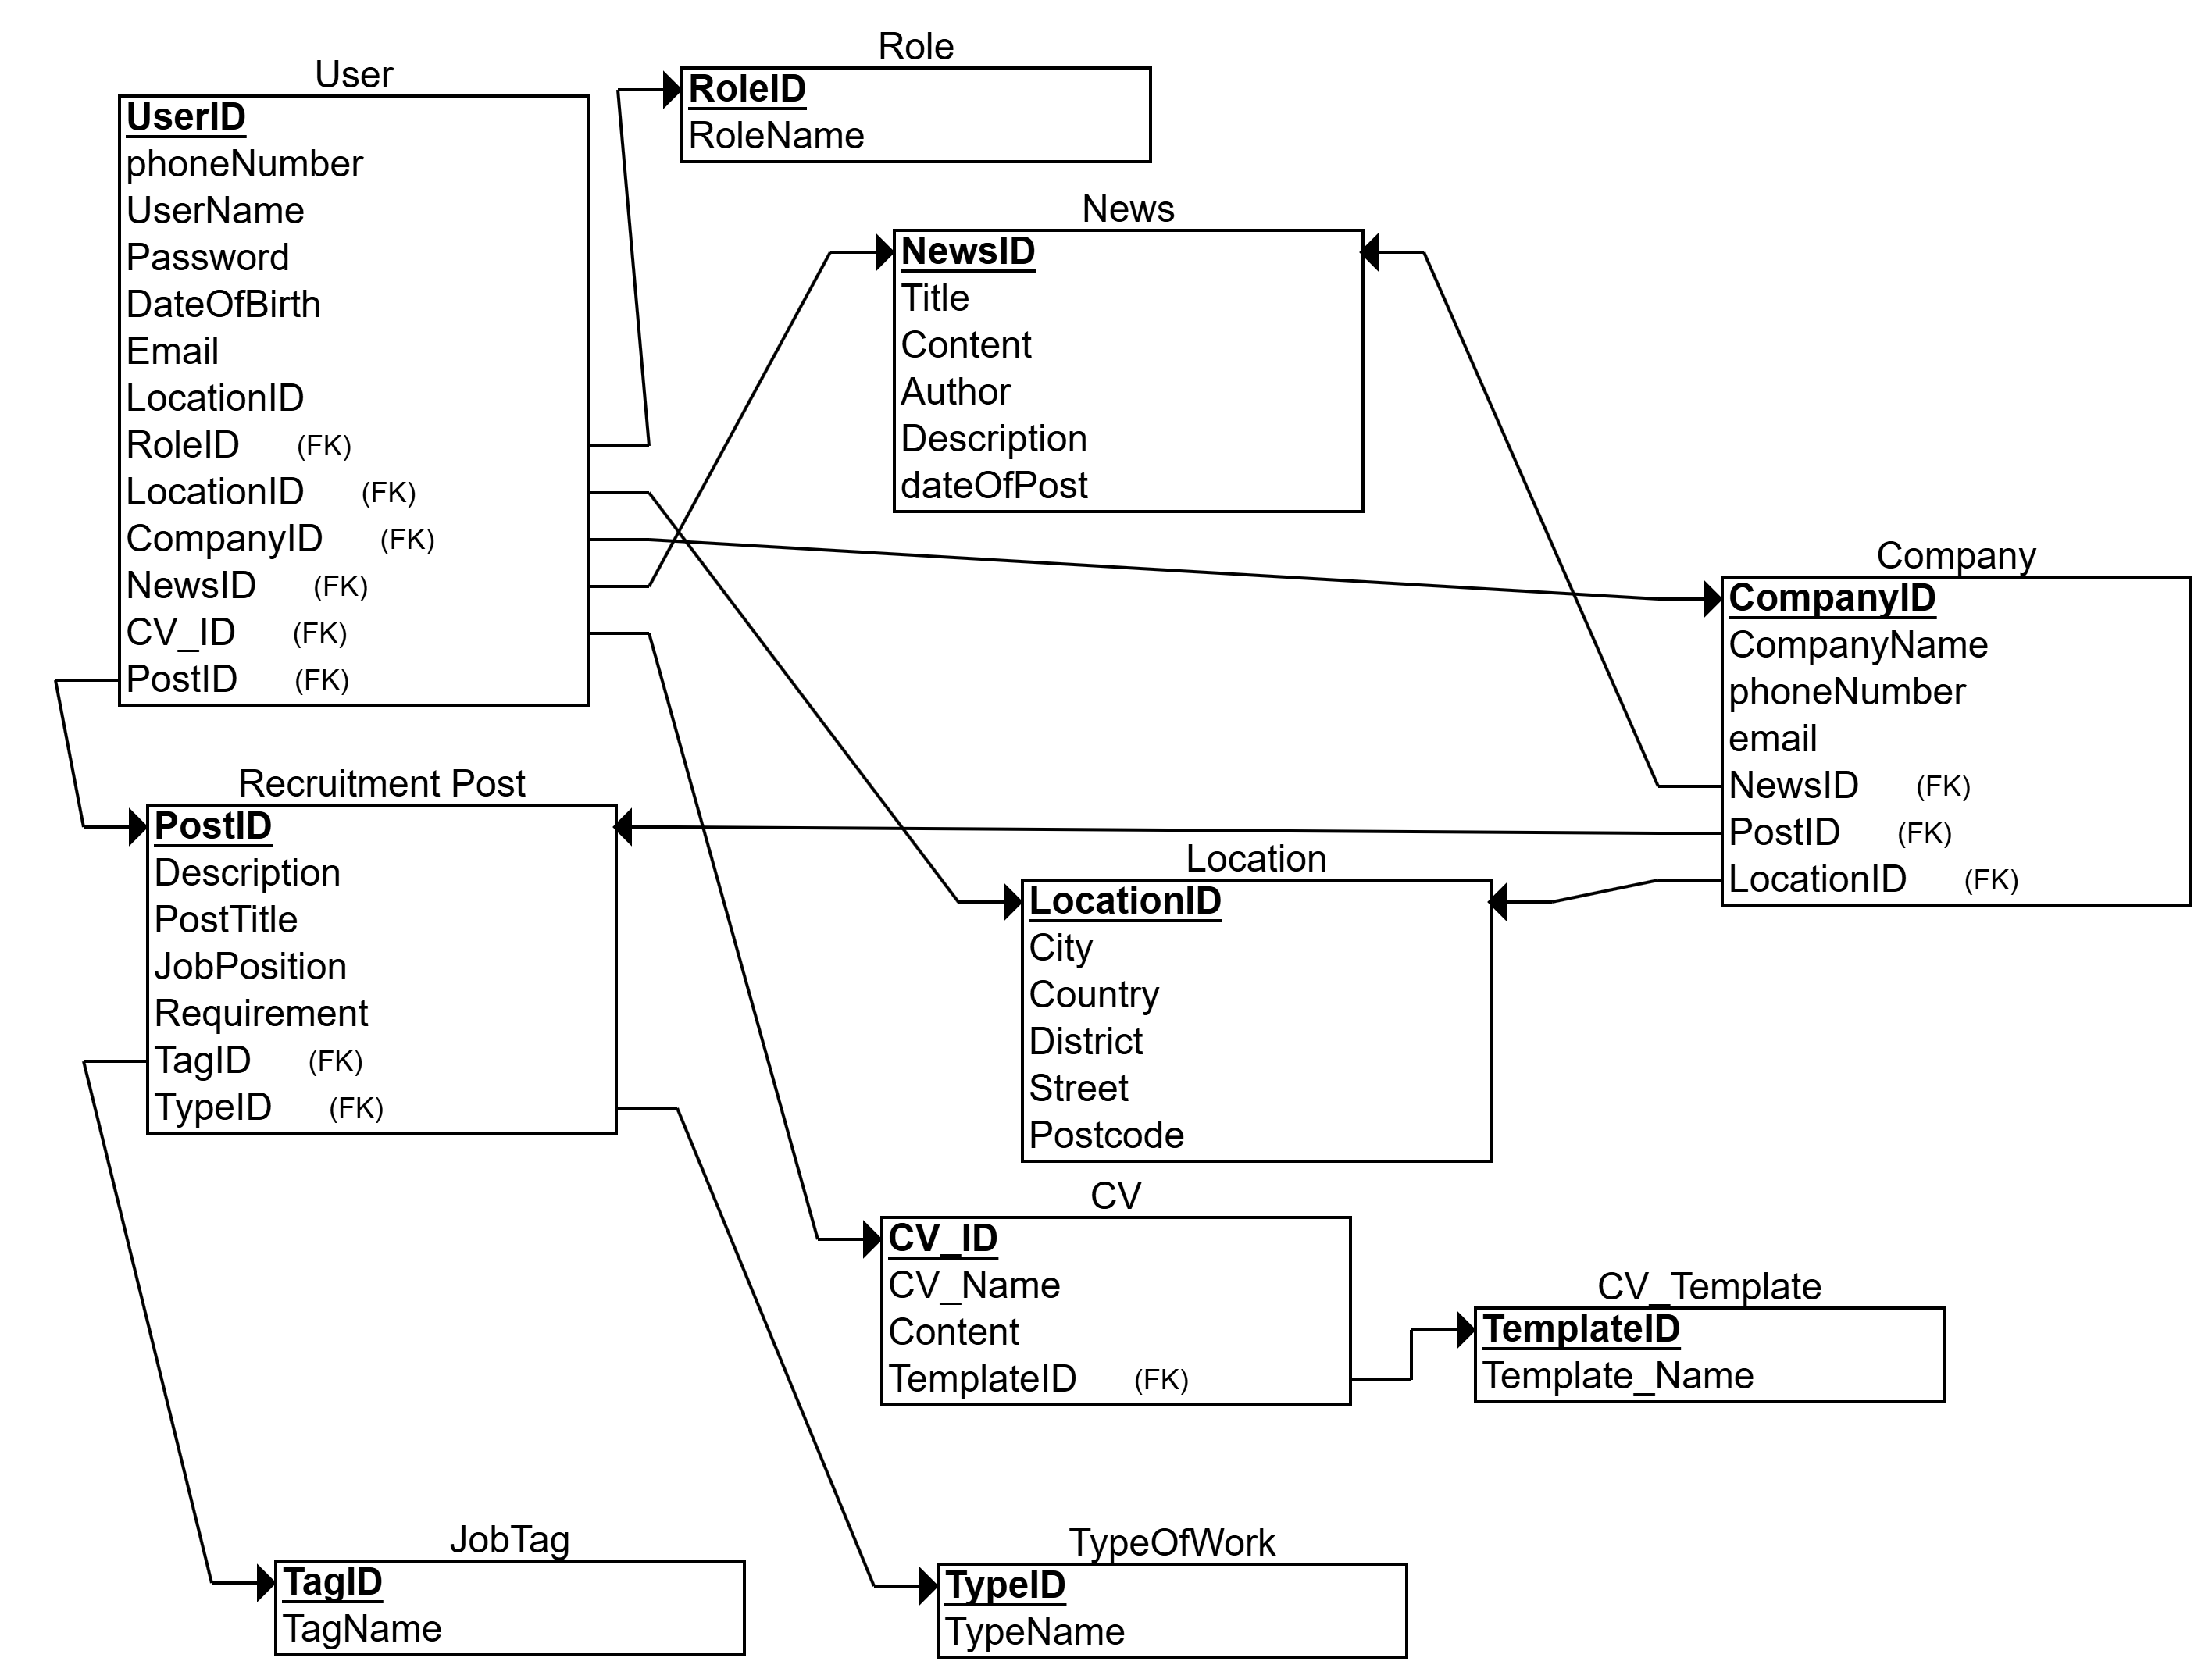
\includegraphics[scale=0.1]{img/Relational_Schema.png}
    \caption{Lược đồ quan hệ}
		
\end{figure}


\chapter{Thiết kế giao diện người diện}

\section{Trang chào mừng}

\begin{figure}[H]
\begin{center}
    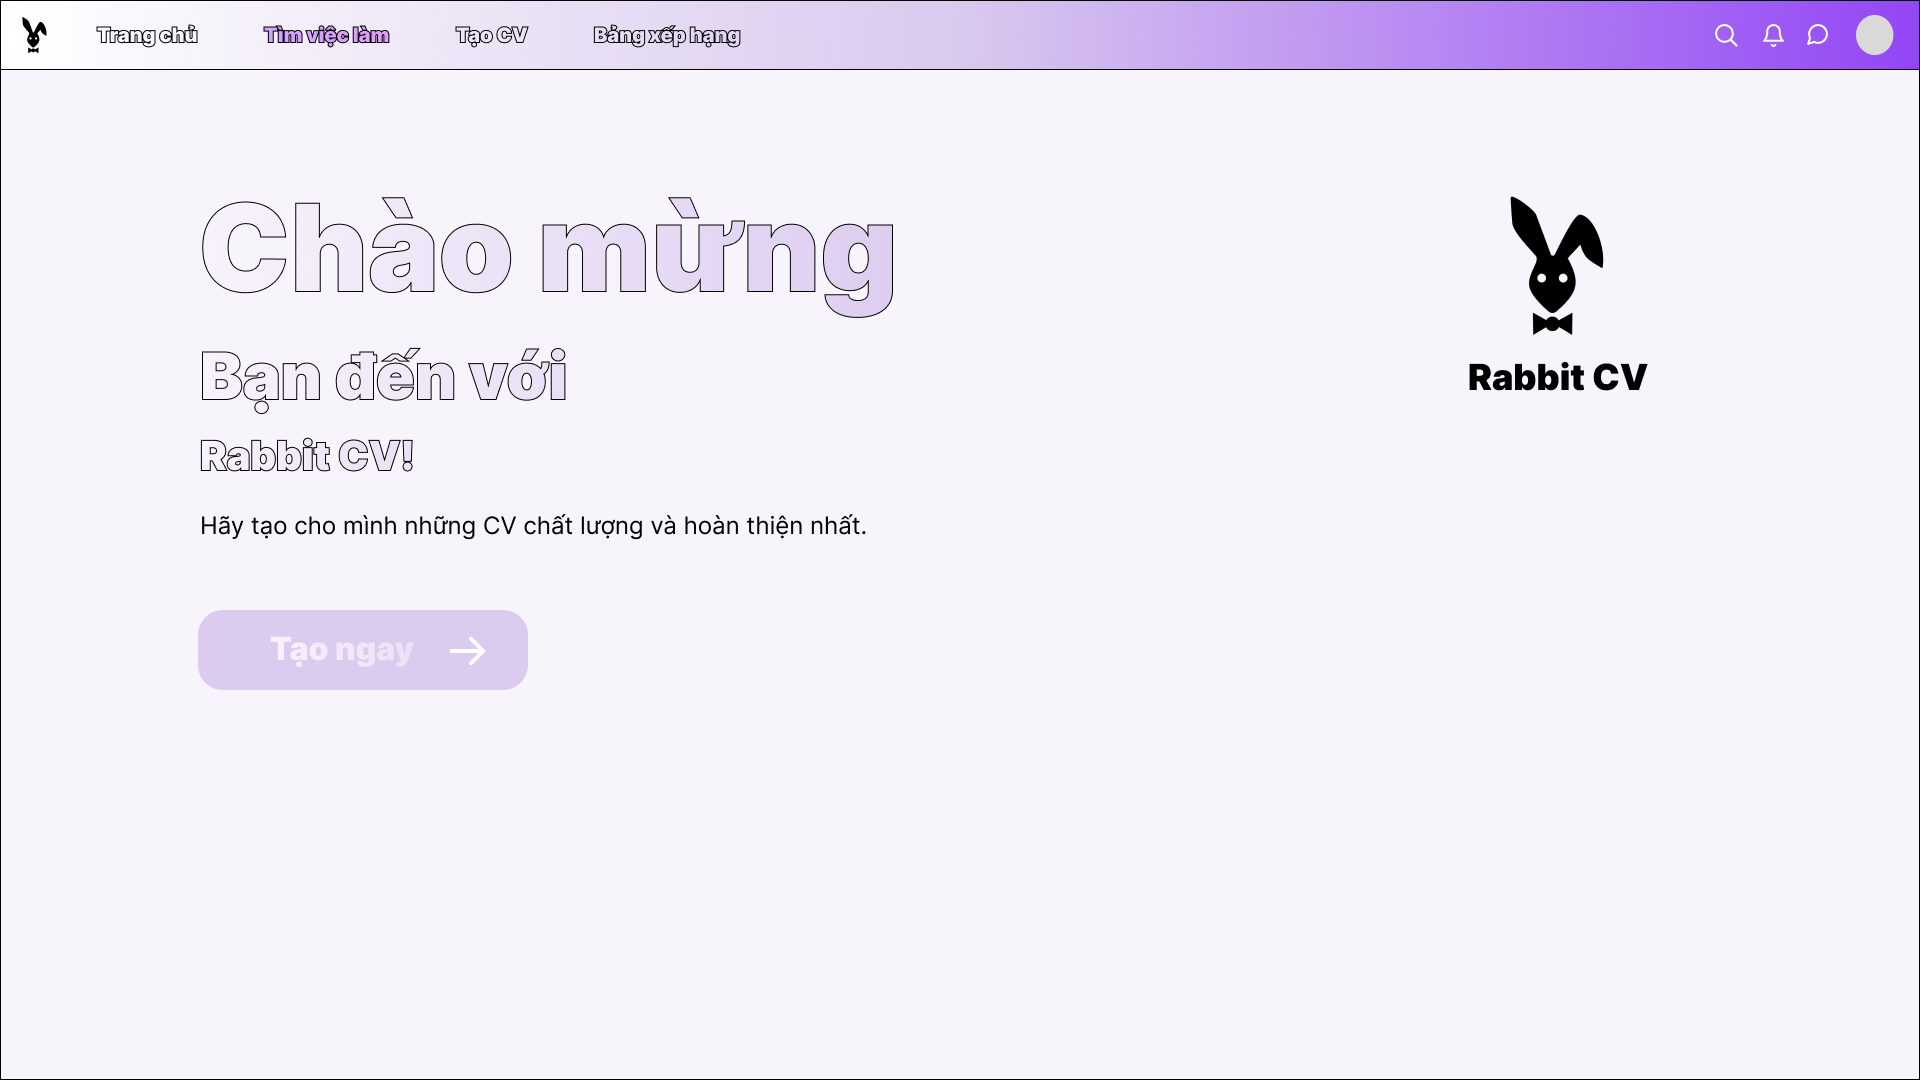
\includegraphics[scale=0.2]{img/Welcome.png}
    \caption{Giao diện của Trang chào mừng}
\end{center}
\end{figure}

Trang chào mừng của một trang web là điểm tiếp xúc đầu tiên giữa người dùng và nội dung của trang web đó. Đây là nơi mà người dùng sẽ có ấn tượng đầu tiên về trang web, và do đó, nó cần phải được thiết kế một cách cẩn thận và chuyên nghiệp.

Trang chào mừng của một trang web đóng vai trò quan trọng trong việc tạo ấn tượng đầu tiên với người dùng. Đây là nơi mà người dùng sẽ quyết định liệu họ có muốn tiếp tục khám phá trang web hay không. Một trang chào mừng hiệu quả không chỉ cần có thiết kế đẹp mắt mà còn phải cung cấp thông tin rõ ràng và dễ hiểu về nội dung và mục đích của trang web. 

Do đó, việc thiết kế giao diện của trang chào mừng cần phải thân thiện với người dùng và dễ dàng điều hướng.

\section{Trang đăng nhập}

\begin{figure}[H]
\begin{center}
    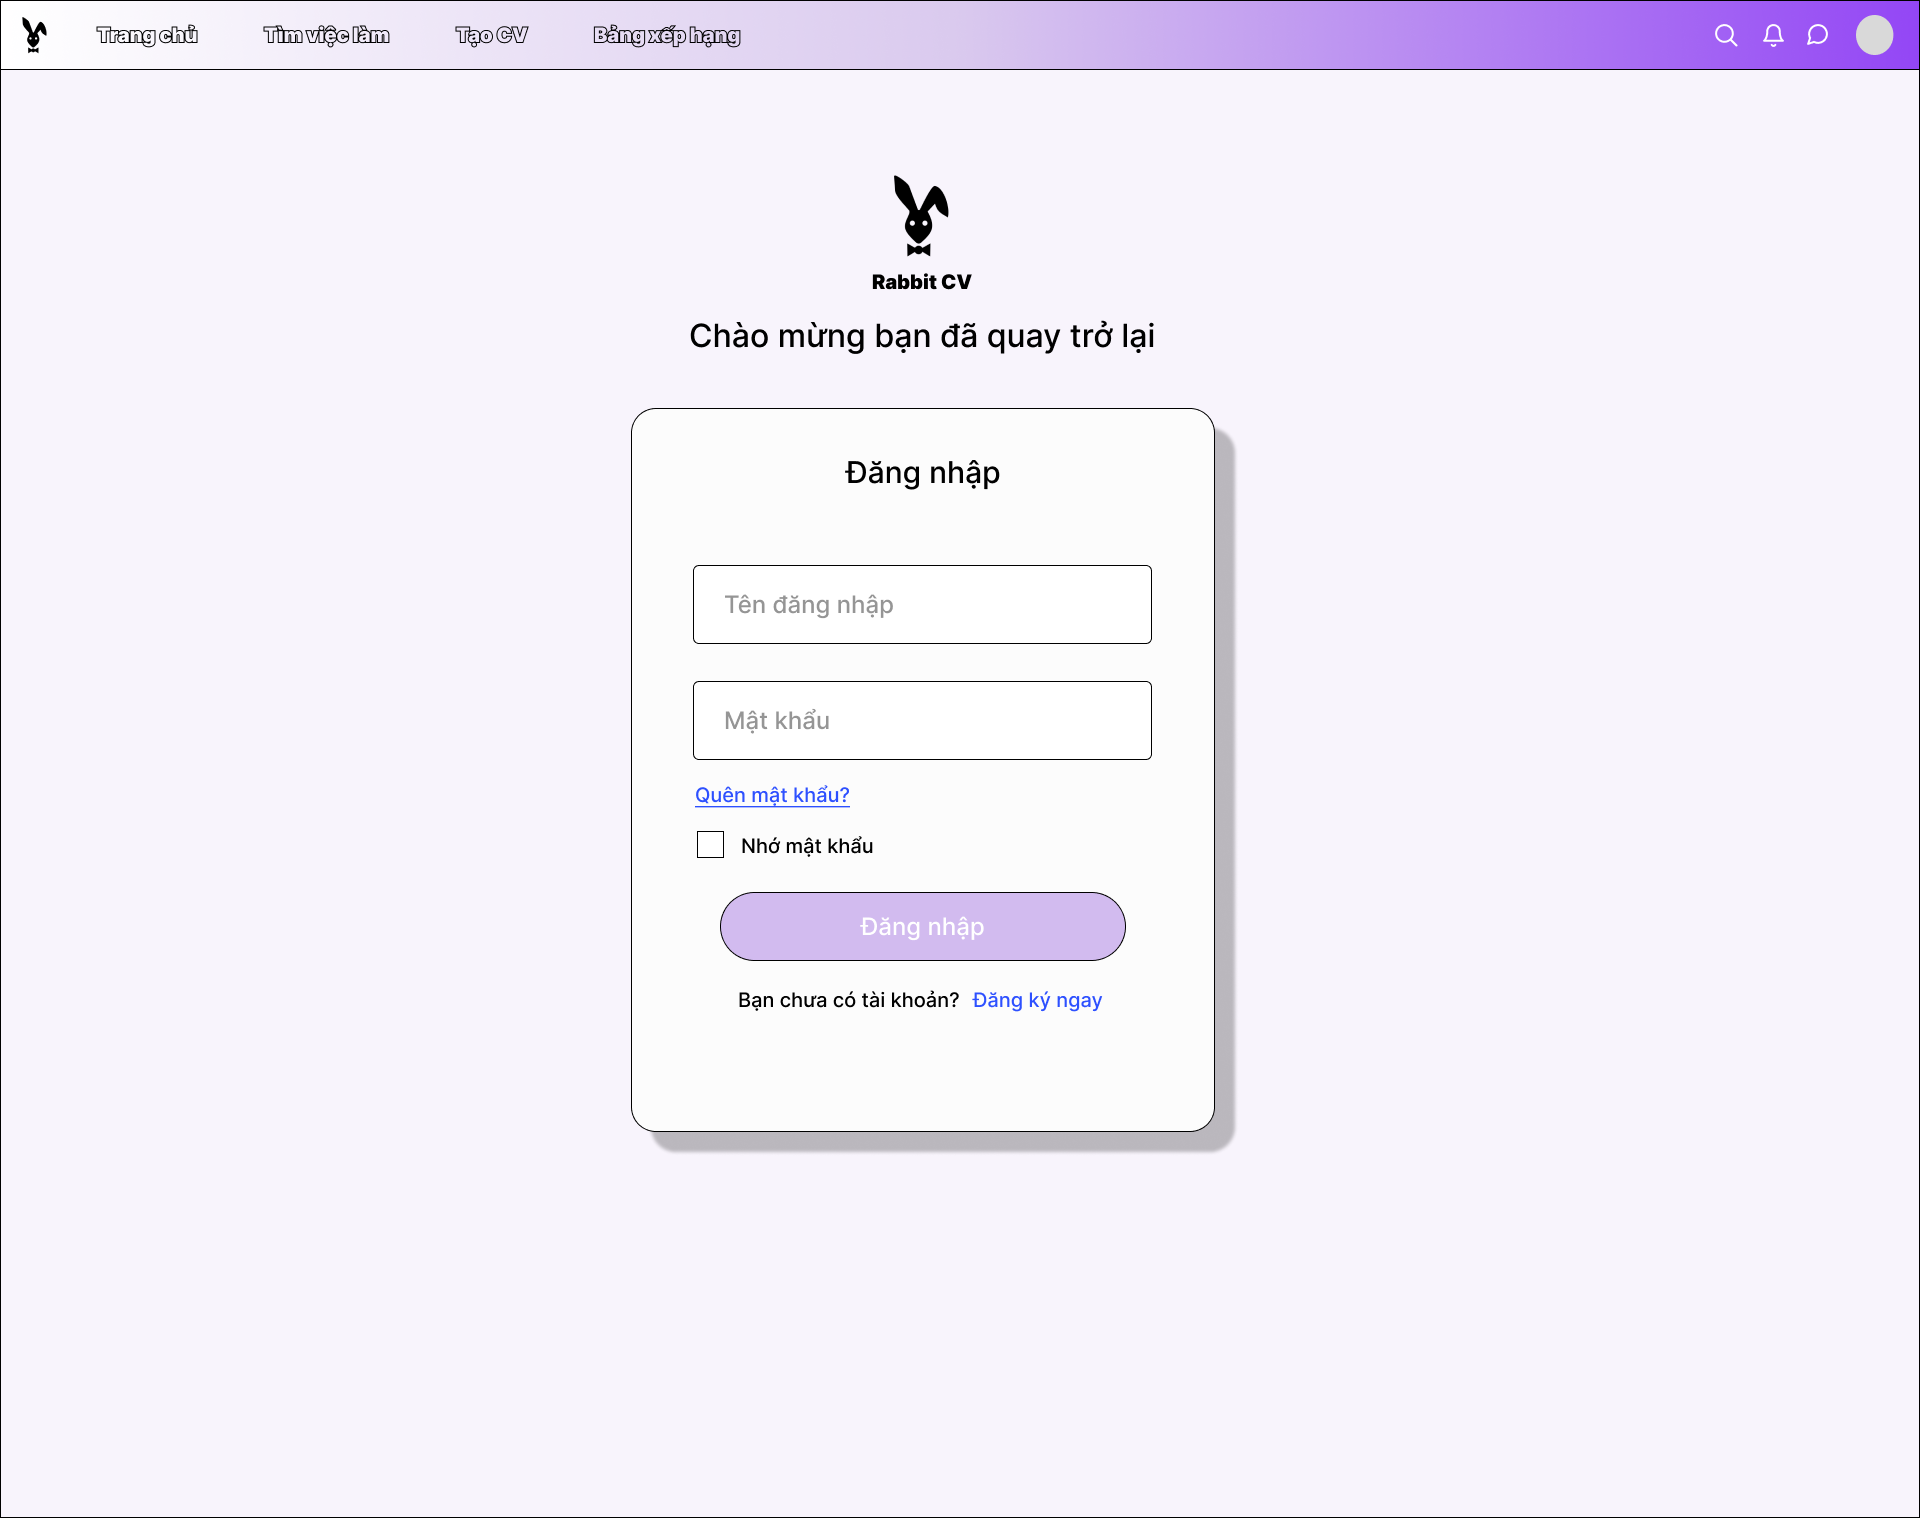
\includegraphics[scale=0.2]{img/Login.png}
    \caption{Giao diện của Trang đăng nhập}
\end{center}
\end{figure}

Trang đăng nhập là một phần quan trọng của bất kỳ trang web hoặc ứng dụng nào yêu cầu người dùng xác thực danh tính trước khi truy cập vào các tính năng hoặc dữ liệu cá nhân. Trang đăng nhập cũng có nhiều tuỳ chọn khác như: "Đăng ký tài khoản mới", "Quên tài khoản",.... 

Trang đăng nhập bao gồm các thành phần:

\begin{itemize}
    \item \textbf{Tên đăng nhập:} người dùng được yêu cầu phải điền vào trang web.
    \item \textbf{Mật khẩu:} Được yêu cầu điền để kiểm tra mật khẩu ứng với tên đăng nhập trong cơ sở dữ liệu.
    \item \textbf{Quên mật khẩu:} Là một đường link được chuyển hướng đến trang "Quên mật khẩu" khi người dùng thực sự quên mật khẩu, tài khoản của mình.
    \item \textbf{Nhớ mật khẩu:} Là một tuỳ chọn giúp người dùng có thể tự động đăng nhập ở các phiên đăng nhập sau.
    \item \textbf{Đăng nhập:} Là một nút để đăng nhập khi người dùng đã điền thông tin tài khoản và mật khẩu. Khi đăng nhập, hệ thông sẽ kiểm tra tài khoản và mật khẩu của người dùng có trong cơ sở dữ liệu của hệ thống hay không.
    \item \textbf{Đăng ký ngay:} Là đường link chuyển hướng tới trang "Đăng ký tài khoản". Nếu người dùng vẫn chưa có tài khoản trong cơ sở dữ liệu của hệ thống, người dùng có thể lựa chọn tuỳ chọn này để tạo tài khoản mới.
\end{itemize}

\section{Trang đăng ký}

\begin{figure}[H]
\begin{center}
    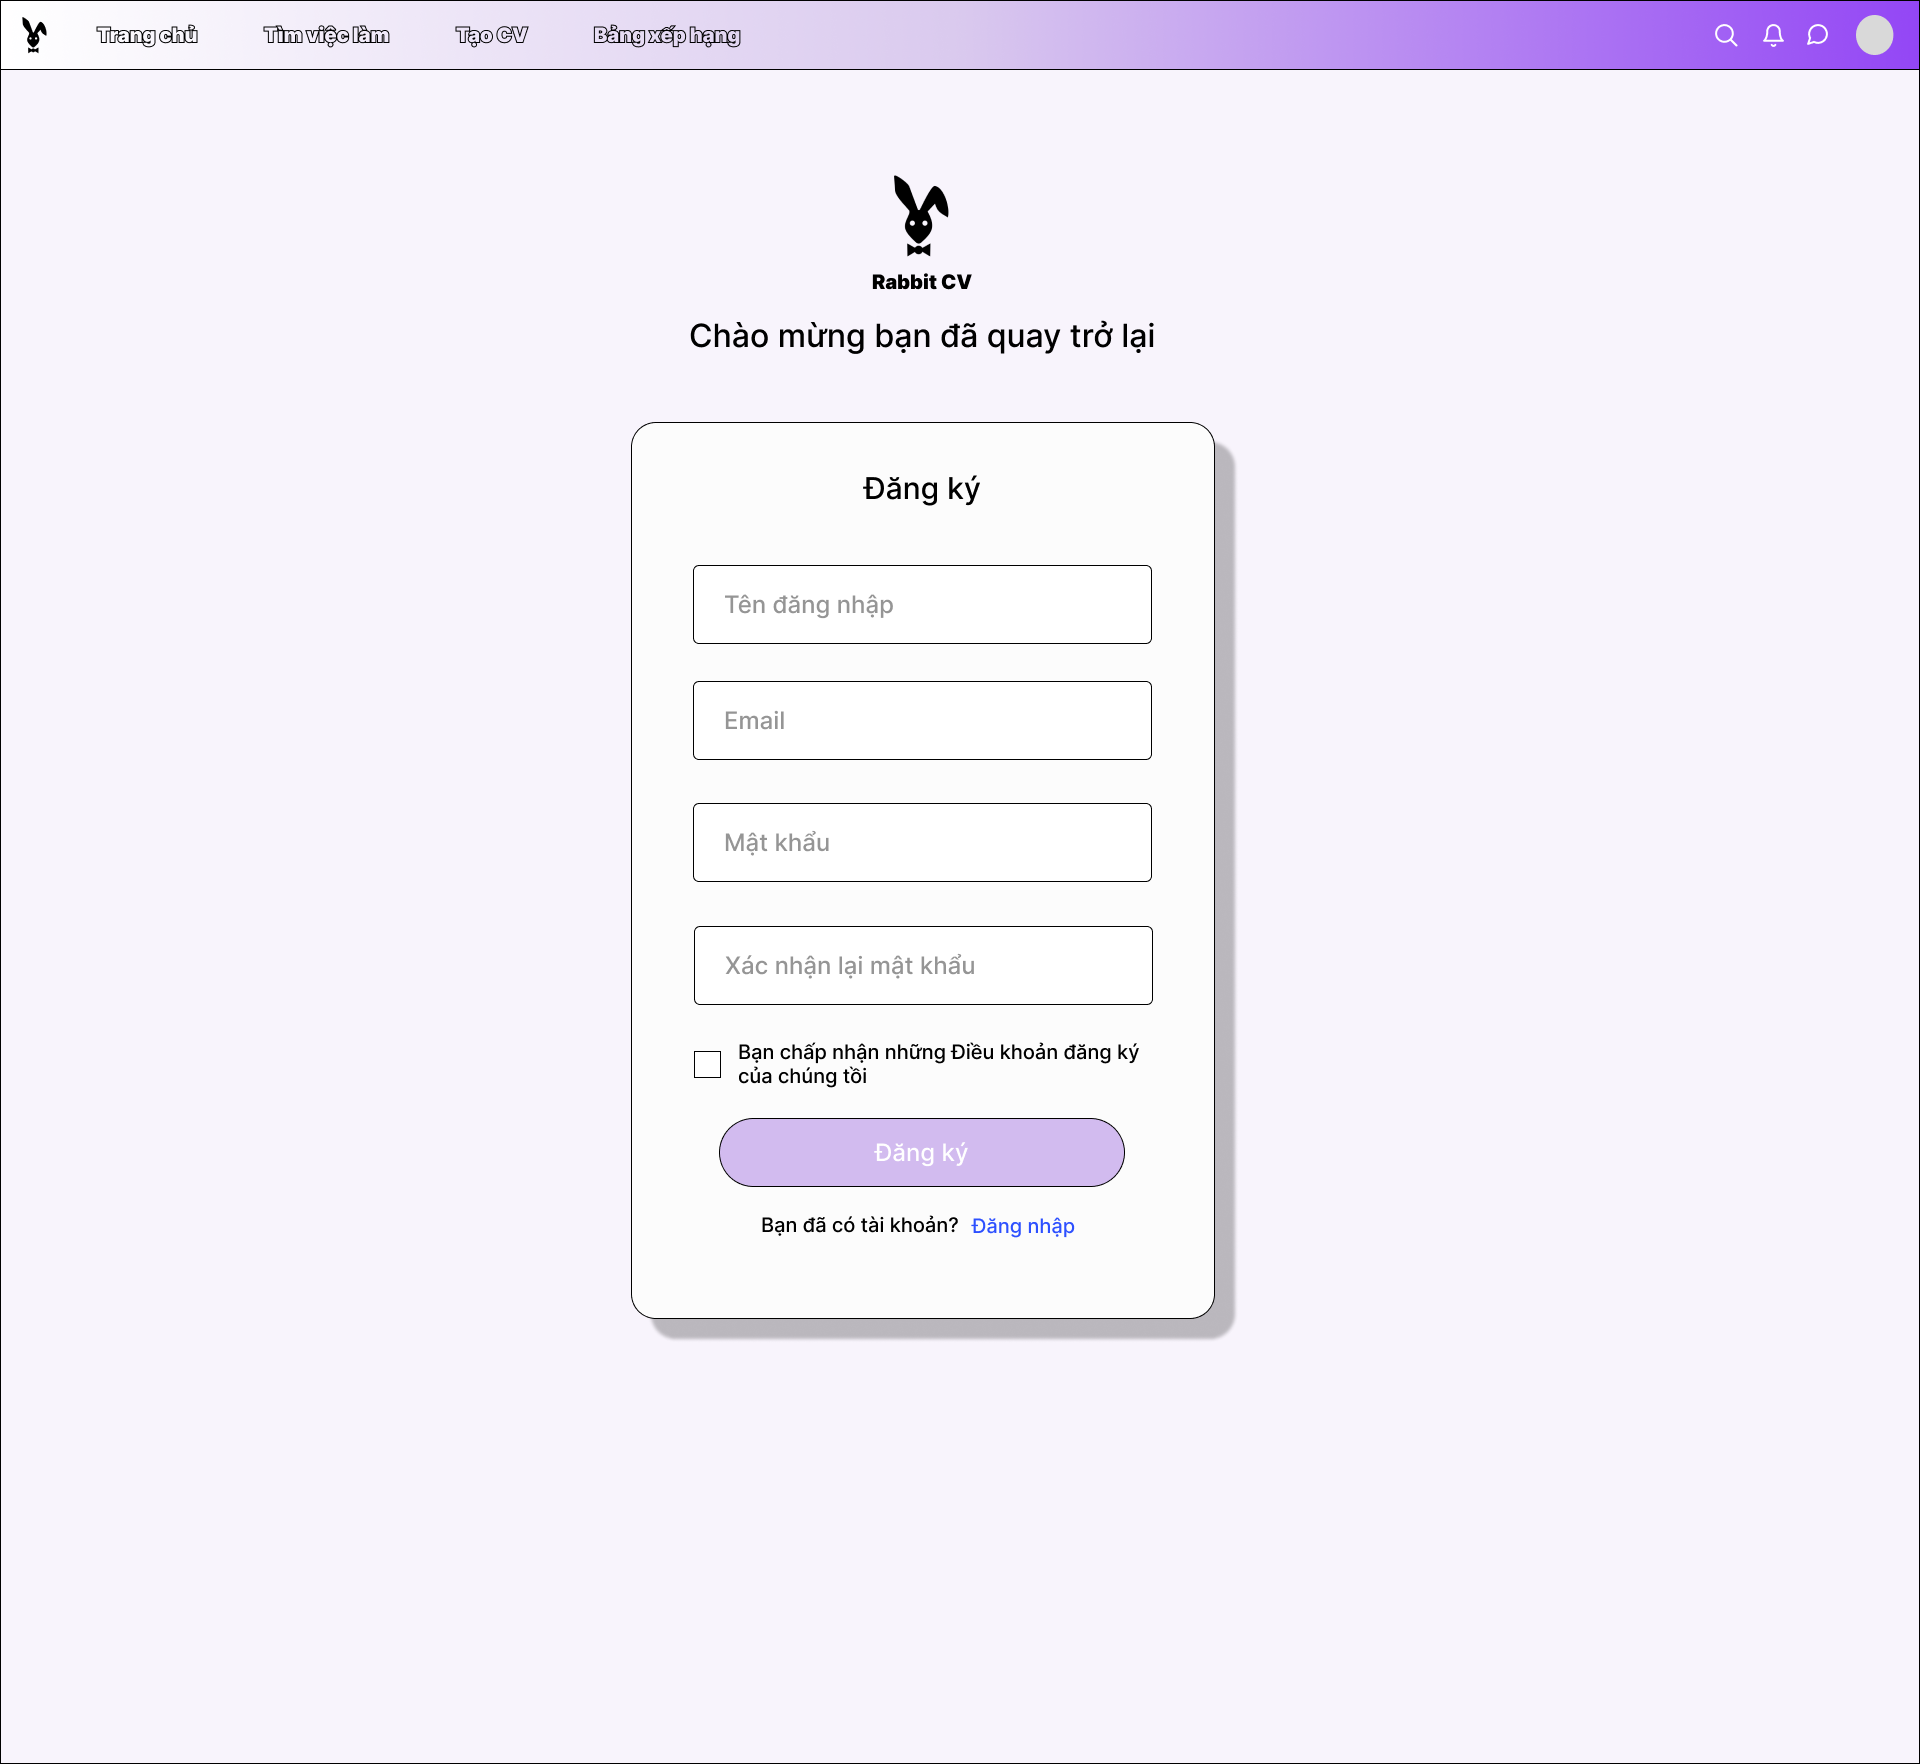
\includegraphics[scale=0.2]{img/Register.png}
    \caption{Giao diện Trang đăng ký}
\end{center}
\end{figure}

Là trang web yêu cầu người dùng tạo tài khoản mới để có truy cập vào các tính năng và dịch vụ của trang web. Để đăng ký tài khoản mới, người dùng cần phải đồng ý với các điều khoản, điều kiện đăng ký của trang web.

Trang đăng ký có các thành phần:
\begin{itemize}
    \item \textbf{Tên đăng nhập:} Là trường yêu cầu người dùng phải nhập tên đăng nhập của mình. 
    \item \textbf{Email:} Là trường người dùng được yêu cầu phải nhập để sau này khi người dùng quên mật khẩu, hệ thống có thể dựa vào đó để xác minh người dùng.
    \item \textbf{Mật khẩu:} Là trường để người dùng đặt mật khẩu. Ở trường này, mật khẩu sẽ được dấu dưới dạng ký hiệu *, để dấu mật khẩu trước những người khác ở trước màn hình. Người dùng cũng có thể lựa chọn nhìn mật khẩu nếu họ thực sự muốn.
    \item \textbf{Xác nhận mật khẩu:} Là trường để xác nhận lại với người dùng mật khẩu mà họ đã chọn .
    \item \textbf{Đăng ký:} Là nút khi người dùng nhấn vào, hệ thống sẽ kiểm tra lại cơ sở dữ liệu xem tài khoản mà người dùng chọn đã có người khác xài chưa. Nếu đã có, thì hệ thống sẽ thông báo "Tạo tài khoản thất bại" và yêu cầu người chọn một tên tài khoản khác. Còn nếu chưa, hệ thống sẽ thông báo "Tạo tài khoản thành công" và đưa người dùng đến trang đăng nhập.
    \item \textbf{Đăng nhập:} Là đường link chuyển hướng người dùng đến trang "Đăng nhập". Nếu người dùng đã có tài khoản trong cơ sở dữ liệu của hệ thống, họ có thể lựa chọn chức năng này.
\end{itemize}


\section{Trang chủ}

\begin{figure}[H]
\begin{center}
    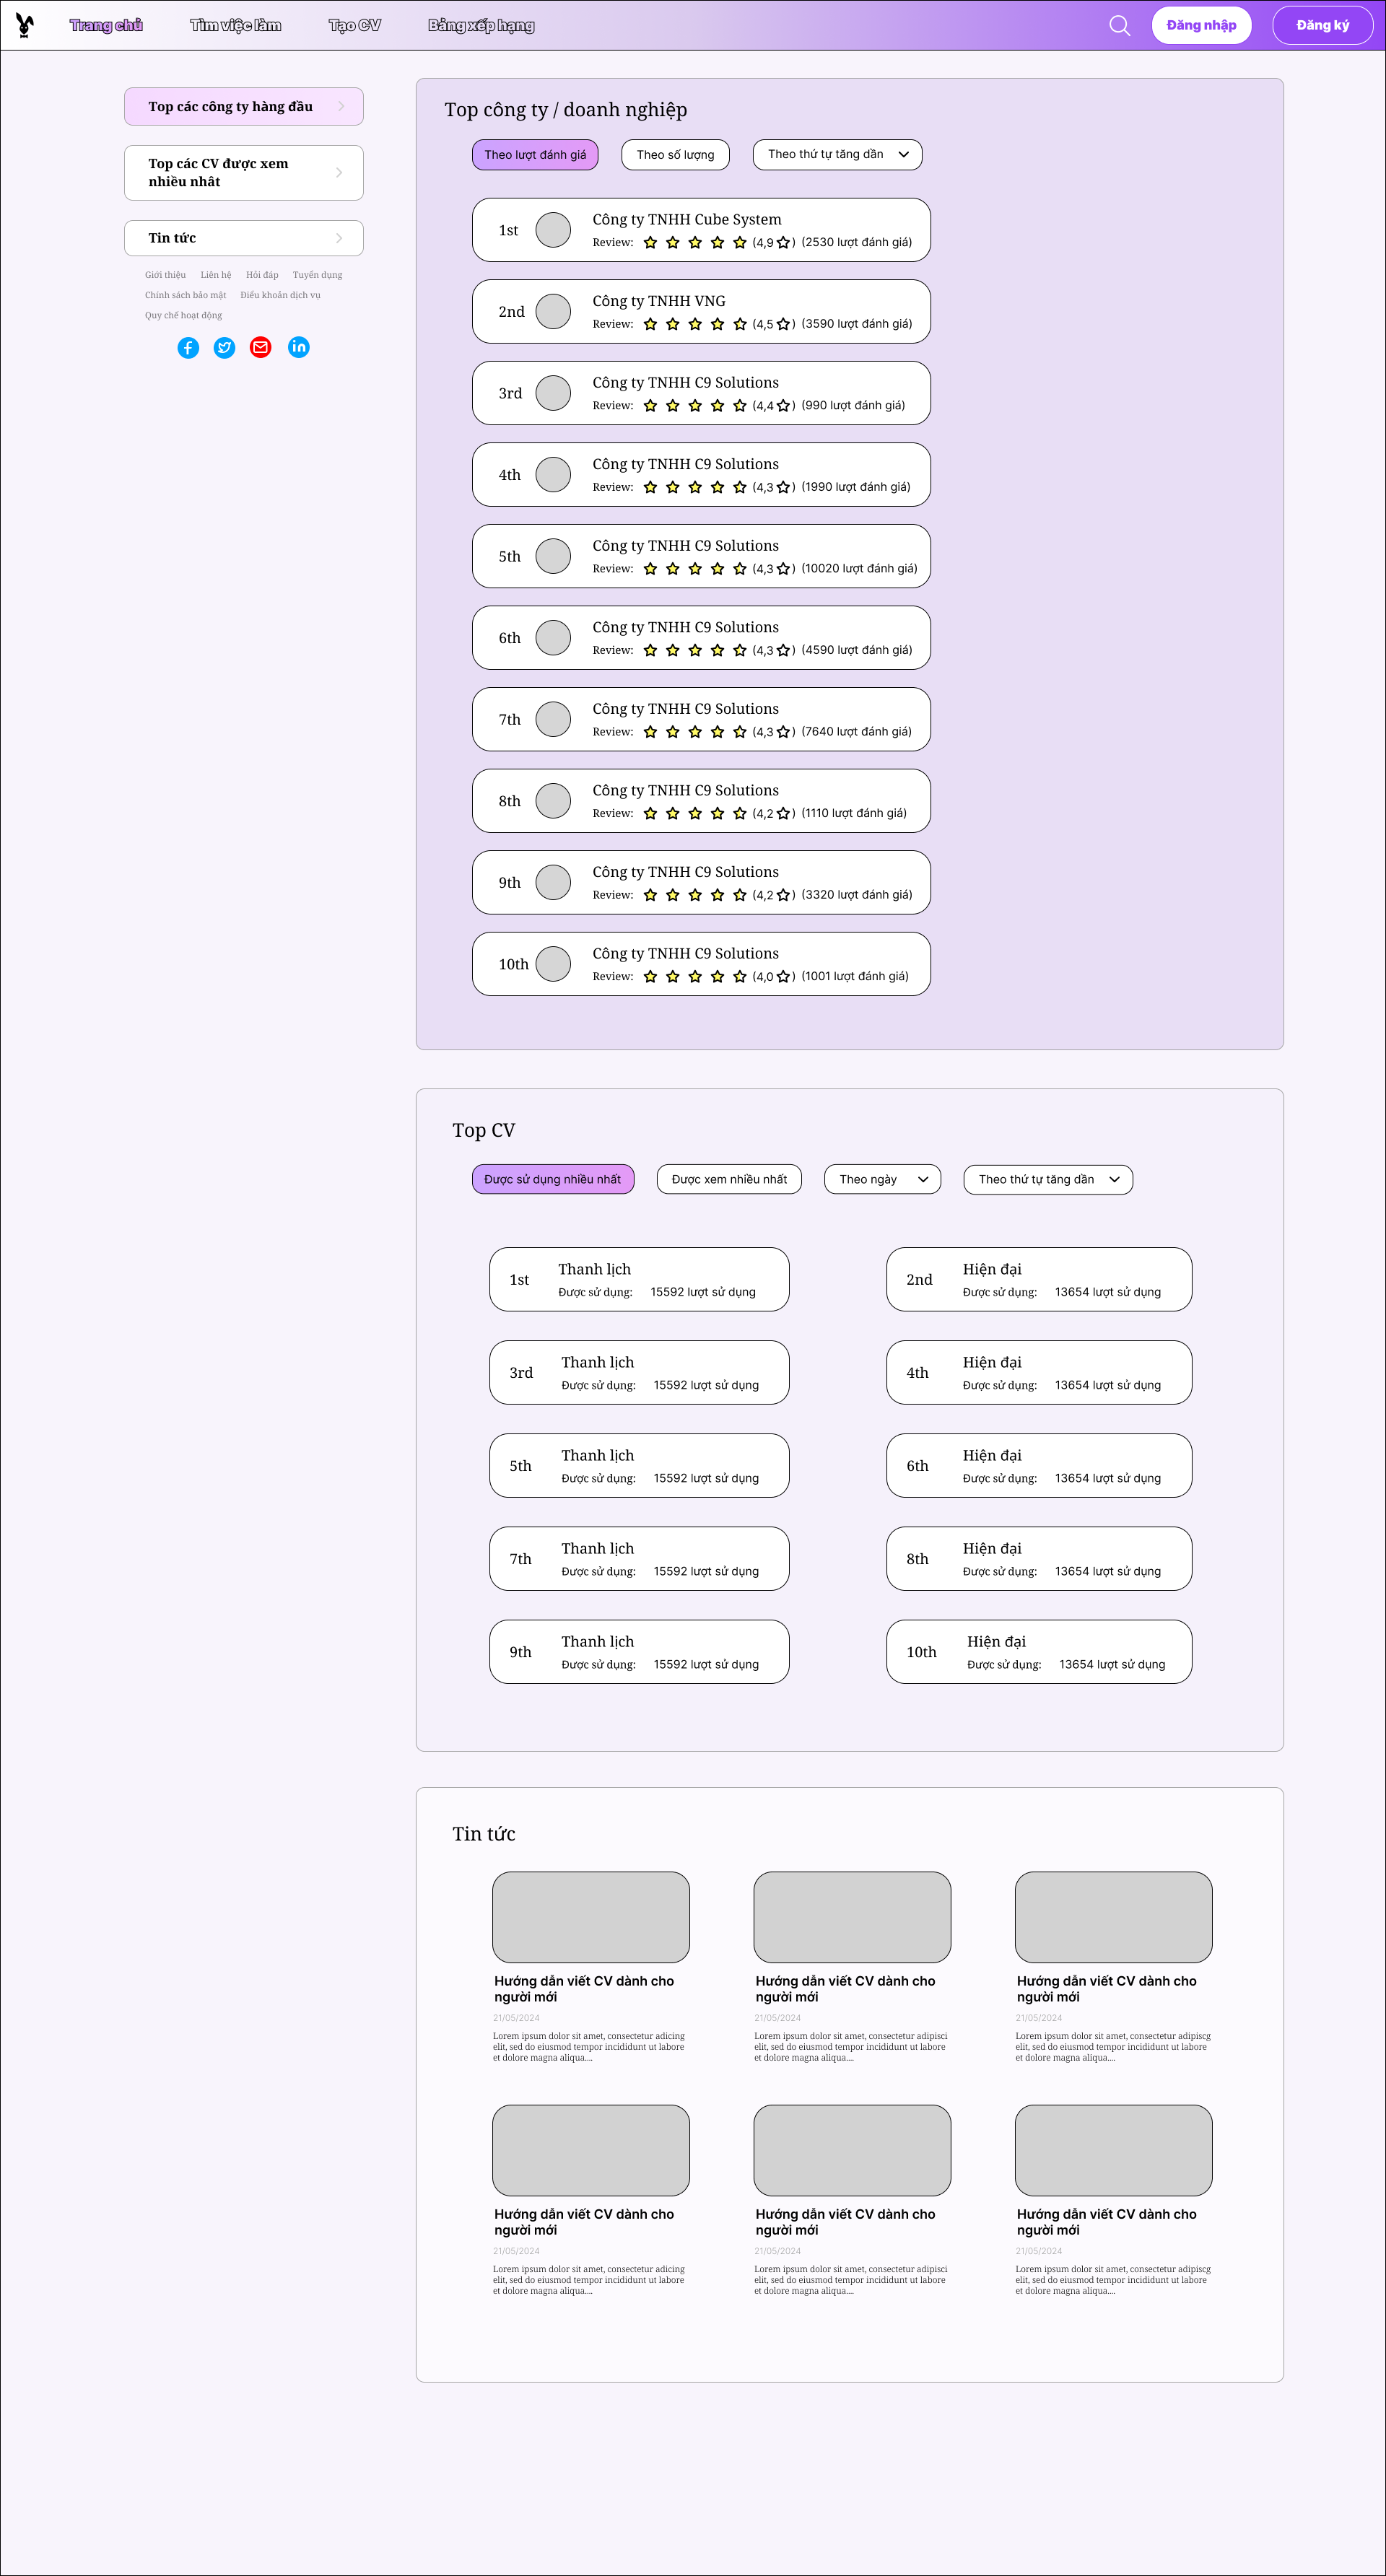
\includegraphics[scale=0.15]{img/Homepage.png}
    \caption{Giao diện của Trang chủ}
\end{center}
\end{figure}

Trang chủ của một trang web là điểm đầu tiên và quan trọng nhất mà người dùng sẽ truy cập. Đây là nơi cung cấp cái nhìn tổng quan về nội dung và dịch vụ mà trang web cung cấp. Trang web này cũng là cổng thông tin chính giúp người dùng dễ dàng điều hướng và tìm kiếm thông tin.

Ở trang web này, gồm có 3 mục: Top doanh nghiệp, Top CV và Tin tức. Ở mảng bên trái sẽ có một danh sách gồm các danh mục vừa được nêu giúp người dùng có thể chọn và nhanh chóng di chuyển đến mục đã được chọn.


\section{Trang tìm kiếm công việc}

\begin{figure}[H]
\begin{center}
    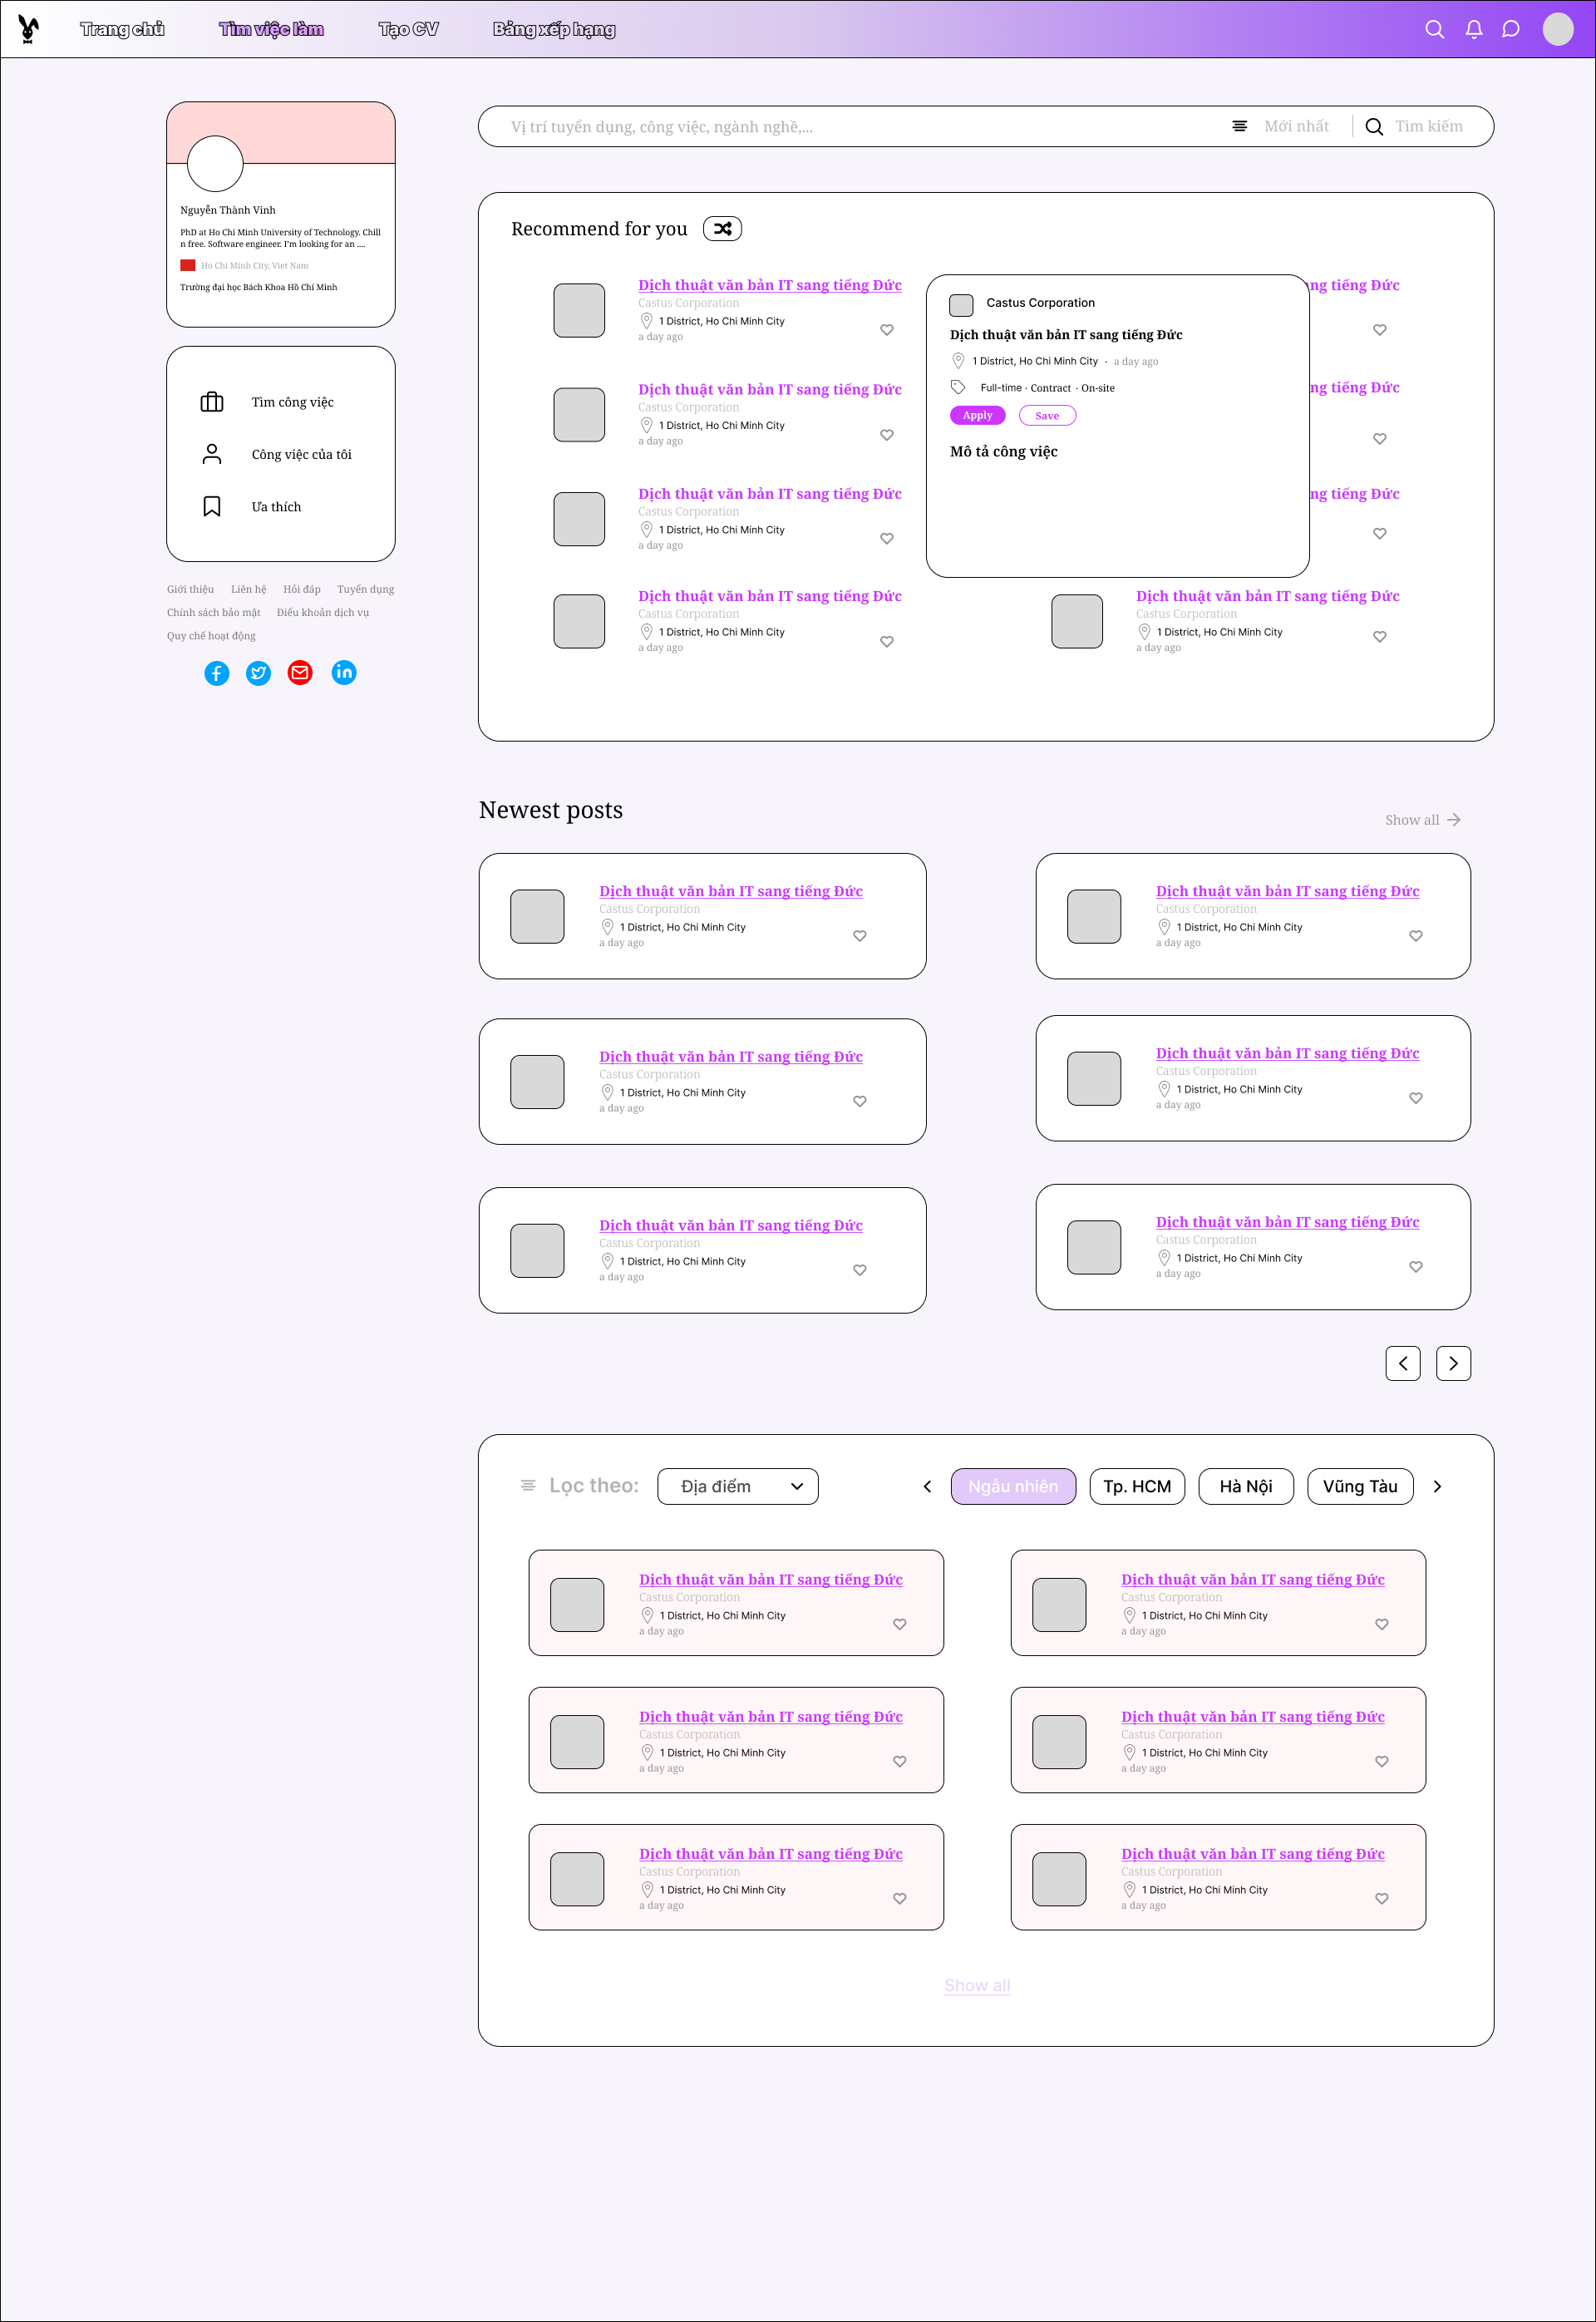
\includegraphics[scale=0.2]{img/FindingJob.png}
    \caption{Giao diện của Trang tìm kiếm công việc}
\end{center}
\end{figure}

Trang tìm kiếm công việc là trang hiển thị những bài đăng tuyển dụng của các doanh nghiệp. Ở đây, có 3 phần: "Recommend for you" gồm những bài đăng ngẫu nhiên được hệ thống đưa lên hệ thống, "Newest posts" gồm những bài đăng mới nhất, gần đây nhất và mục lọc danh sách những bài đăng tuỳ theo vị trí, lương, kinh nghiệm,.... 

\section{Trang quản lý CV}

\begin{figure}[H]
\begin{center}
    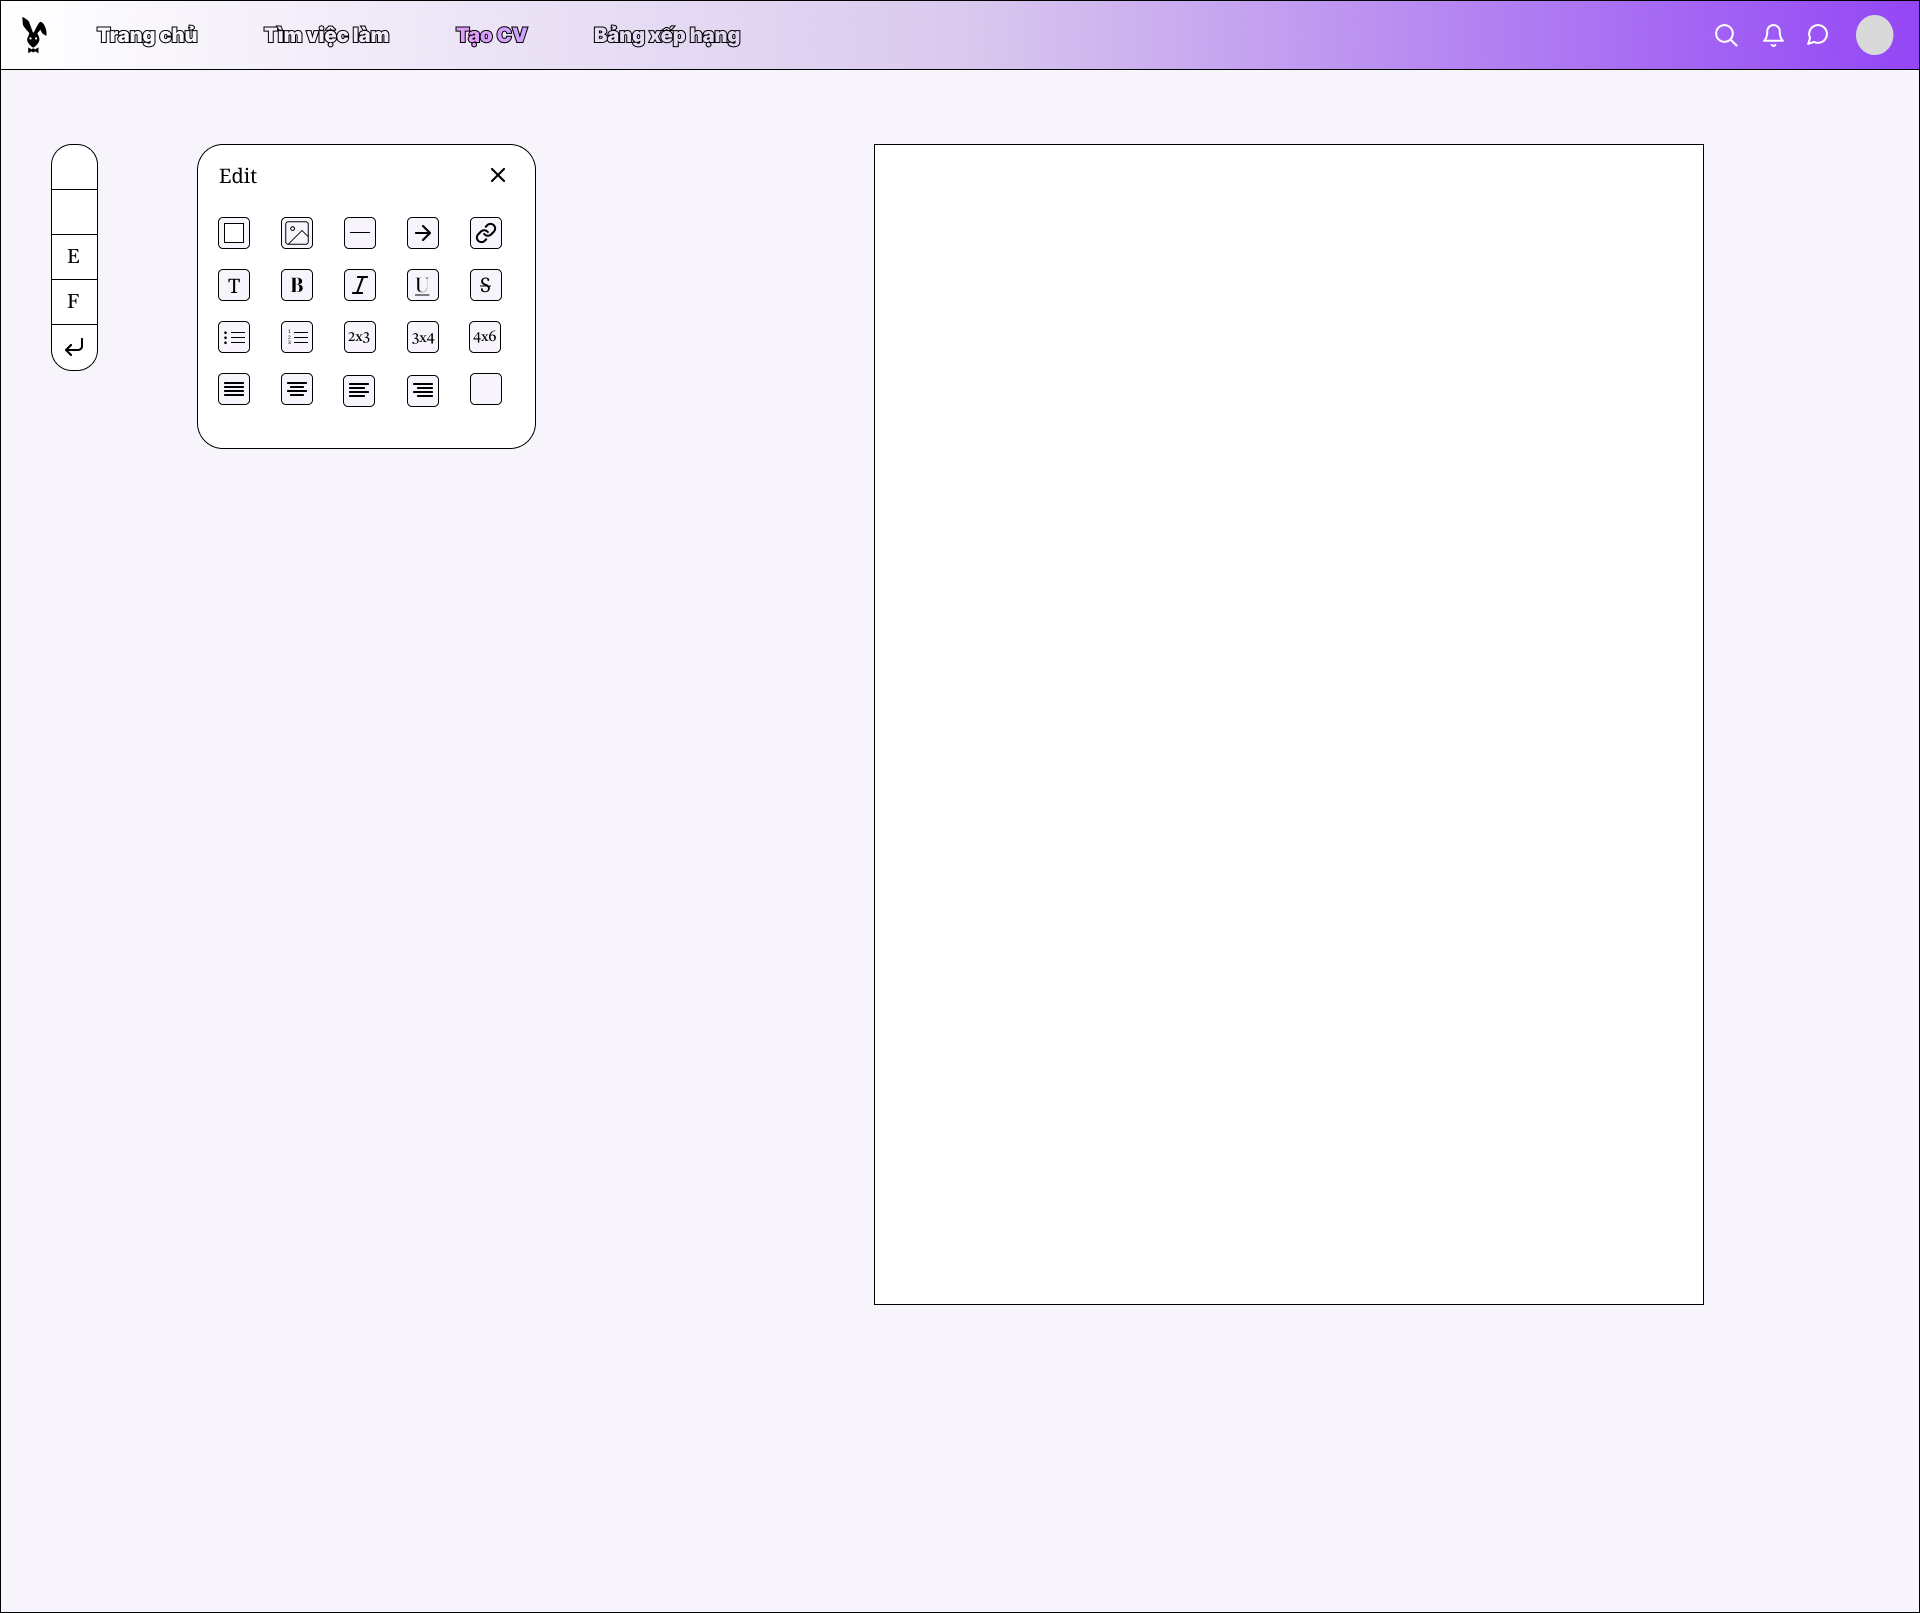
\includegraphics[scale=0.2]{img/CV_Management.png}
    \caption{Giao diện của Trang quản lý CV}
\end{center}
\end{figure}

Là trang để người dùng quản lý CV của mình. Trang này cung cấp cho người dùng các công cụ và tính năng để tạo, chỉnh sửa và xoá CV của họ một cách nhanh chóng và hiệu quả. Trang quản lý CV không chỉ giúp người dùng tạo ra những bản CV ấn tượng mà còn giúp người dùng dễ dàng quản lý và dễ dàng cập nhật thông tin, từ đó, nâng cao cơ hội tìm kiếm việc làm thành công.

Việc chỉnh sửa CV sẽ tuỳ thuộc vào tuỳ chọn mà người dùng đã chọn. Nếu dùng chọn CV template có trên trang web, hệ thống sẽ hiển thị sẵn một bản mẫu CV có sẵn và việc người dùng cần làm là chỉ điền thông tin cần thiết vào CV. Còn nếu người dùng chọn mục "Custom", hệ thống sẽ chỉ hiển thị 1 trang A4 lên trang web và những công cụ hữu ích hỗ trợ người dùng trong việc tự mình chỉnh sửa CV. Ở mục "Custom", người dùng có thể tự do chỉnh sửa, căn chỉnh hình ảnh, cỡ chữ phù hợp với yêu cầu của mình.



\section{Trang quản lý tài khoản}

\begin{figure}[H]
\begin{center}
    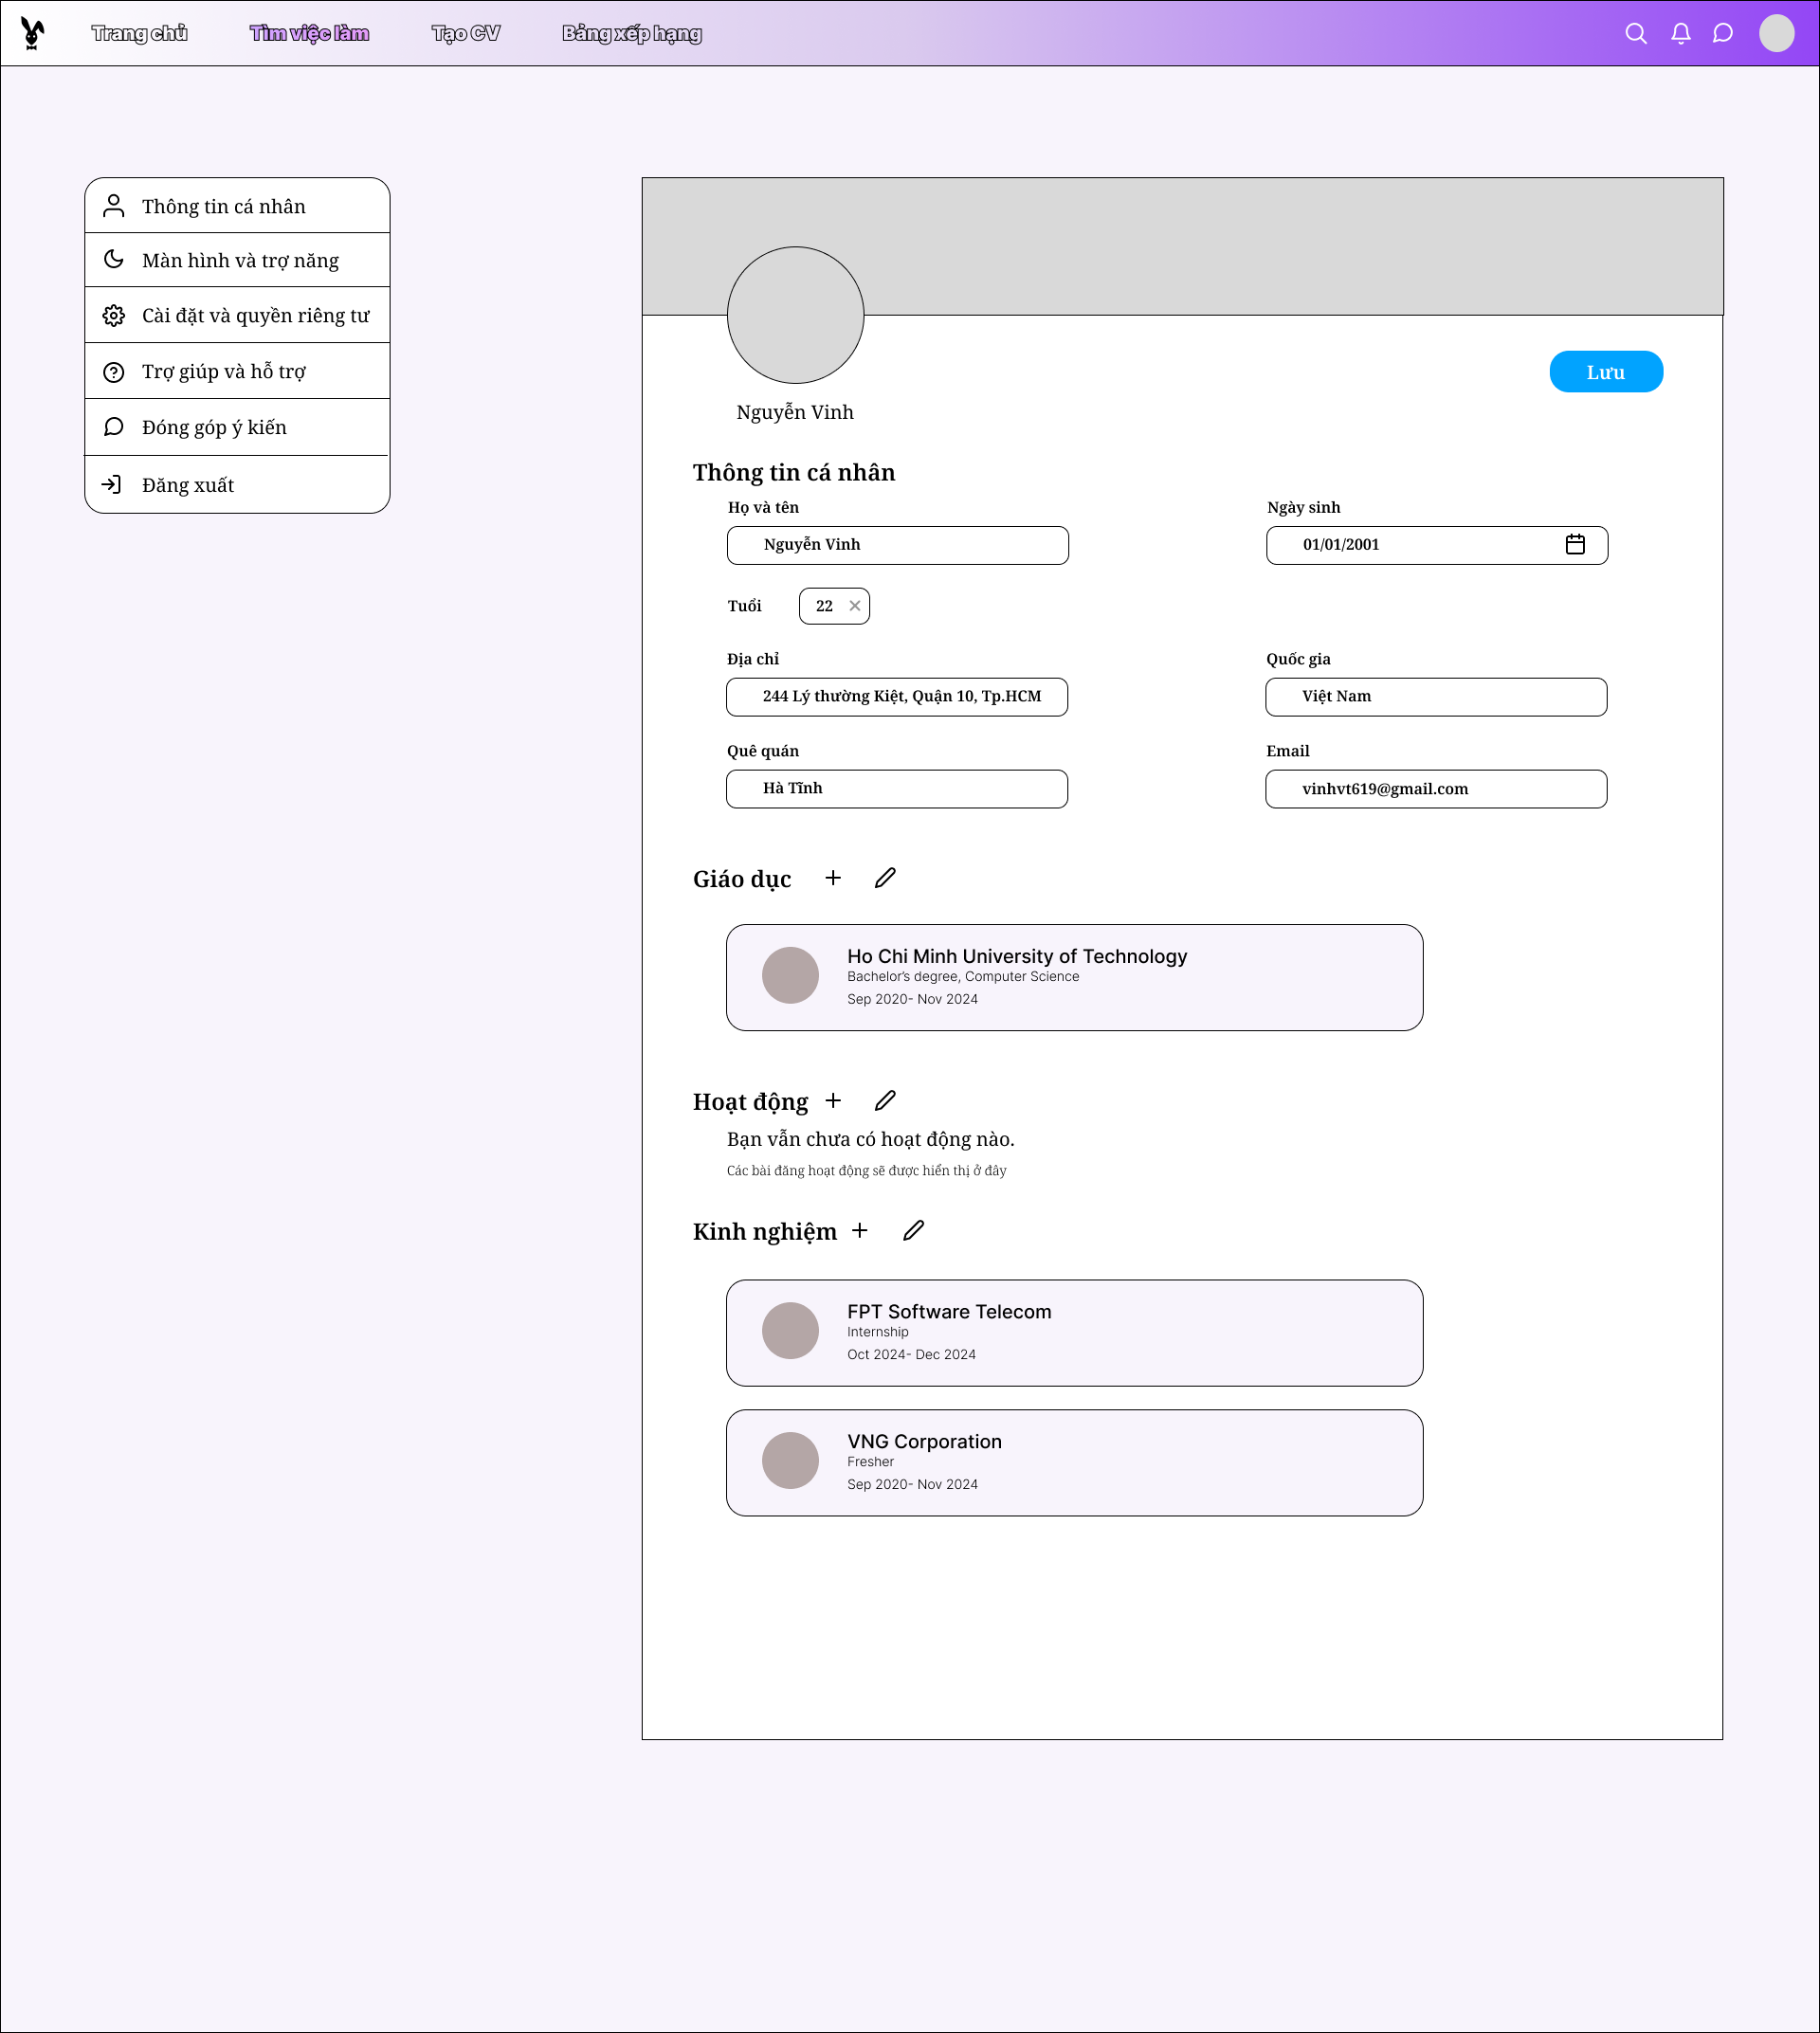
\includegraphics[scale=0.2]{img/ProfileManagement.png}
    \caption{Giao diện của Trang quản lý tài khoản}
\end{center}
\end{figure}

Là trang cài đặt gồm nhiều chức năng quản lý tài khoản. Ở đây, có nhiều mục cho người dùng có thể lựa chọn. Họ có thể lựa chọn để chỉnh sửa thông tin cá nhân của mình và thêm nhiều kỹ năng, kinh nghiệm của mình lên trang web.

Người dùng có thể lựa chọn màn hình tối đối với trang web phù hợp với thị hiếu của mình. Nếu người dùng có bất kỳ vấn đề và cần hỗ trợ hay muốn đóng góp ý kiến bản thân về trang web, họ có thể lựa chọn các mục "Trợ giúp và hỗ trợ" hay "Đóng góp ý kiến". Hệ thống sẽ chuyển hướng người dùng đến trang tương ứng và hướng dẫn người dùng cách thực hiện.
\chapter{Tóm tắt và kế hoạch tương lai}

\section{Đánh giá nhiệm vụ}

Trong quá trình thực hiện đồ án chuyên ngành này, tôi đã đạt được các mục tiêu sau đây:

\begin{itemize}
	\item Xác định mục tiêu, những yêu cầu chức năng và phi chức năng, các bên liên quan của trang web.
	\item Thiết kế các lược đồ usecase, quy trình làm việc, lược đồ lớp, lược đồ tuần tự, cơ sở dữ liệu và hệ thống kiến trúc.
	\item Nghiên cứu và phân tích điểm mạnh, điểm yếu của các công nghệ phù hợp sẽ sử dụng trong đồ án chuyên ngành.
	\item Thiết kế giao diện người dùng, tạo khung dây cho các trang chính.
	\item Phân tích các trang web liên quan, so sánh và cải thiện đối với trang web của mình.
\end{itemize}
\newpage
Dưới đây là kế hoạch cho giai đoạn 1 của Đồ án chuyên ngành:

\begin{figure}[H]
	\centering
	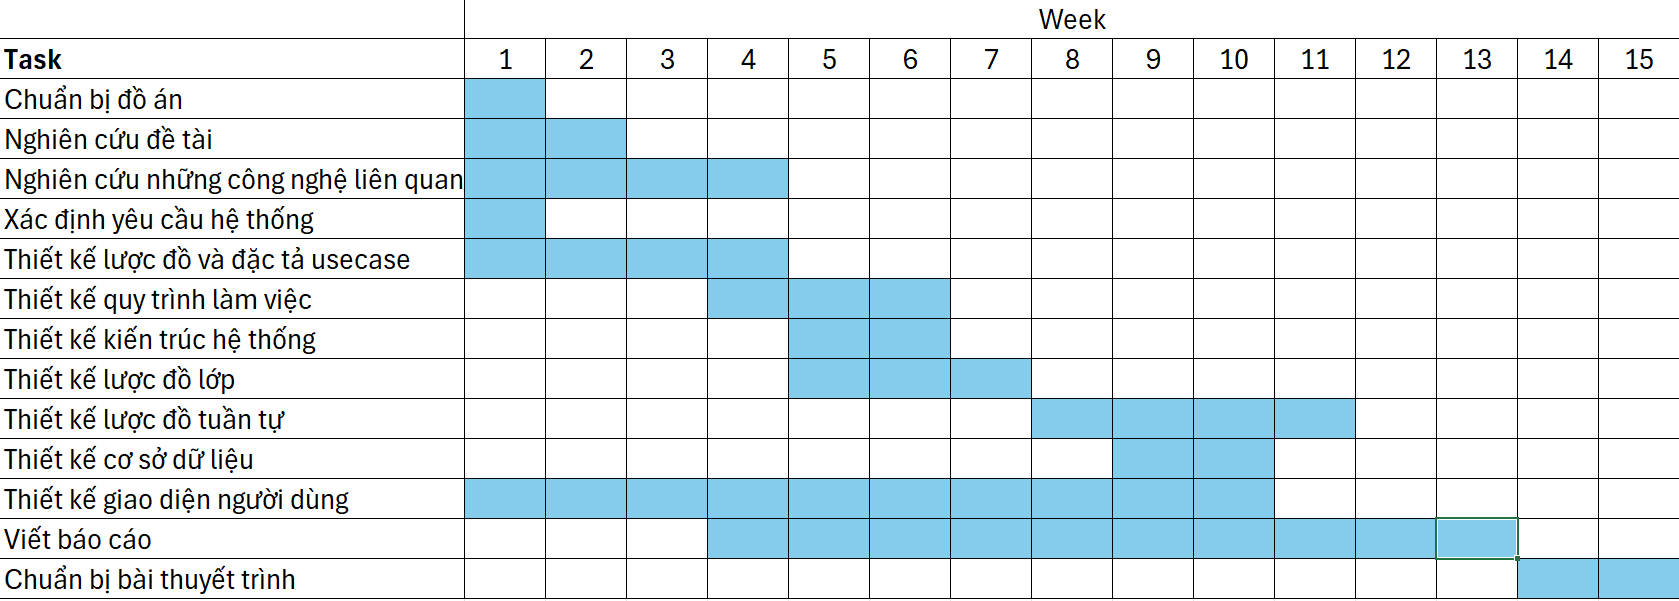
\includegraphics[scale=0.35]{img/TKB_GD1.png}
	\caption{Kế hoạch cho Giai đoạn 1 của Đồ án chuyên ngành}
\end{figure}


\section{Kế hoạch tương lai}

Trong giai đoạn tiếp theo, tôi có kế hoạch dự định hiện thực những chức năng sau:

\begin{itemize}
	\item Trong 2 tuần đầu, tôi sẽ thiết lập môi trường code và thư viện
	\item 4 tuần sau đó, tôi sẽ thiết kế sơ qua những giao diện người dùng đã được vẽ ở trên mà không sử dụng cơ sở dữ liệu.
	\item Vào tuần thứ 6 của đồ án, tôi sẽ nghiên cứu và xây dựng cơ sở dữ liệu cho trang web. Đến tuần thứ 7 sẽ thêm dữ liệu vào database và bắt đầu thử nghiệm thêm API vào trang web. Tuần 8, 9 và 10, tôi sẽ thử nghiệm và sửa lỗi của trang web. Và hoàn thiện những trang chính của trang web.
	\item Đồng thời, ở tuần 8, 9, 10 và 11, tôi nghiên cứu và hiện thức các chức năng liên quan đến CV như: nhập dữ liệu từ file PDF, trích xuất dữ liệu từ hệ thống thành file PDF.
	\item Việc kiếm nghiệm và sửa lỗi trang web sẽ được thực hiện xuyên suốt trong quá trình xây dựng trang web.
	\item Quá trình deploy sẽ được thực hiện ngay khi trang web đã hoàn tất.
\end{itemize}


Dưới đây là kế hoạch cho giai đoạn 2 của Đồ án tốt nghiệp:

\begin{figure}[H]
	\centering
	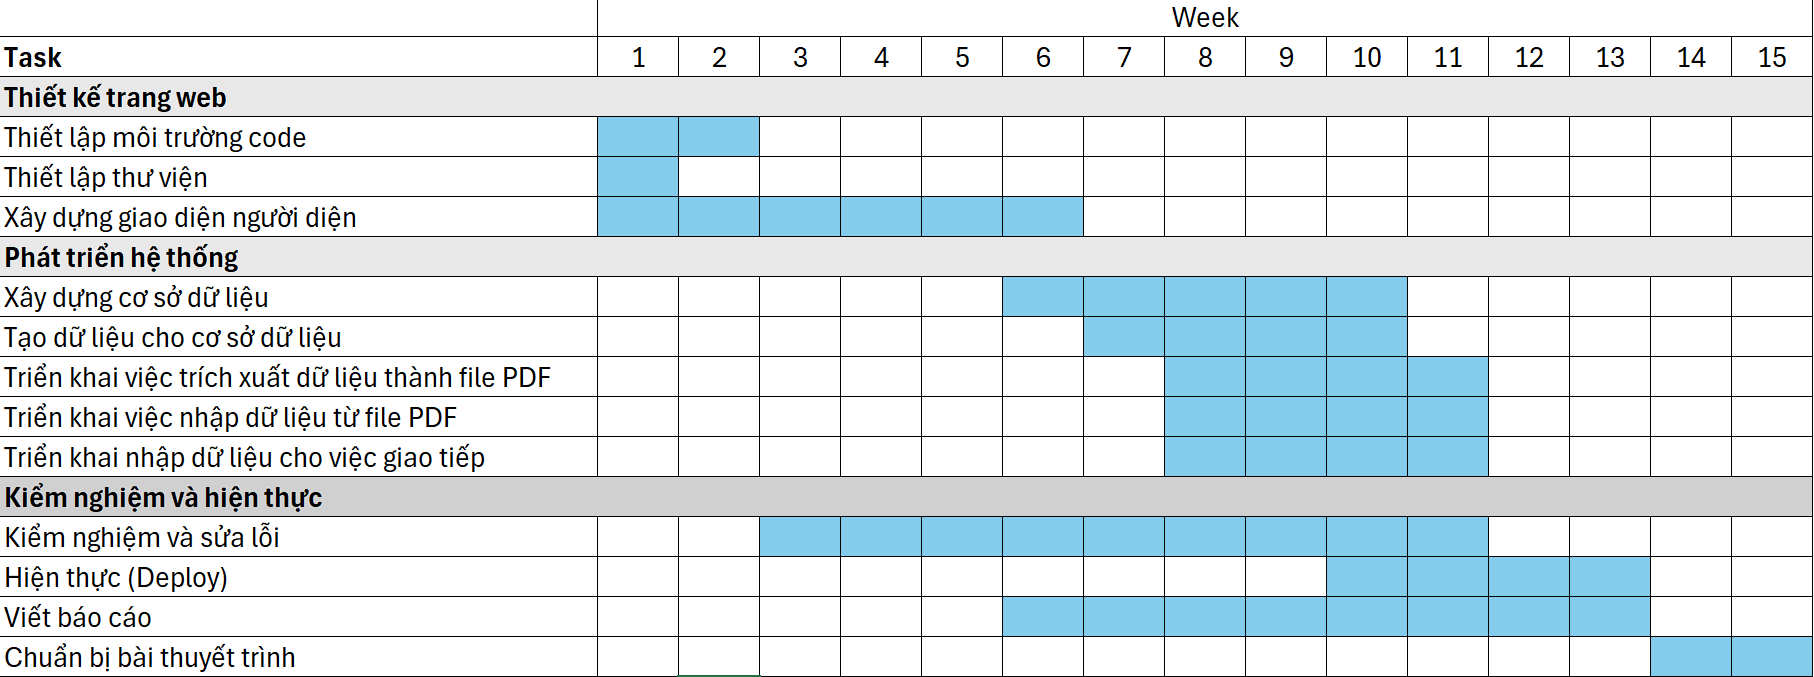
\includegraphics[scale=0.35]{img/TKB_GD2.png}
	\caption{Kế hoạch cho Giai đoạn 2 của Đồ án tốt nghiệp}
\end{figure}
%\input{Chapter3.tex}

%-	Danh mục TL tham khảo
%-	Phụ lục (nếu có)

% comment two lines and use manually.bbl bellow if manually
\bibliographystyle{plain} % ieeetr
\bibliography{refs} 

% un-comment this line to use manually
\input{manually.bbl}

\end{document}